\documentclass[twoside]{book}

% Packages required by doxygen
\usepackage{fixltx2e}
\usepackage{calc}
\usepackage{doxygen}
\usepackage[export]{adjustbox} % also loads graphicx
\usepackage{graphicx}
\usepackage[utf8]{inputenc}
\usepackage{makeidx}
\usepackage{multicol}
\usepackage{multirow}
\PassOptionsToPackage{warn}{textcomp}
\usepackage{textcomp}
\usepackage[nointegrals]{wasysym}
\usepackage[table]{xcolor}

% Font selection
\usepackage[T1]{fontenc}
\usepackage[scaled=.90]{helvet}
\usepackage{courier}
\usepackage{amssymb}
\usepackage{sectsty}
\renewcommand{\familydefault}{\sfdefault}
\allsectionsfont{%
  \fontseries{bc}\selectfont%
  \color{darkgray}%
}
\renewcommand{\DoxyLabelFont}{%
  \fontseries{bc}\selectfont%
  \color{darkgray}%
}
\newcommand{\+}{\discretionary{\mbox{\scriptsize$\hookleftarrow$}}{}{}}

% Page & text layout
\usepackage{geometry}
\geometry{%
  a4paper,%
  top=2.5cm,%
  bottom=2.5cm,%
  left=2.5cm,%
  right=2.5cm%
}
\tolerance=750
\hfuzz=15pt
\hbadness=750
\setlength{\emergencystretch}{15pt}
\setlength{\parindent}{0cm}
\setlength{\parskip}{3ex plus 2ex minus 2ex}
\makeatletter
\renewcommand{\paragraph}{%
  \@startsection{paragraph}{4}{0ex}{-1.0ex}{1.0ex}{%
    \normalfont\normalsize\bfseries\SS@parafont%
  }%
}
\renewcommand{\subparagraph}{%
  \@startsection{subparagraph}{5}{0ex}{-1.0ex}{1.0ex}{%
    \normalfont\normalsize\bfseries\SS@subparafont%
  }%
}
\makeatother

% Headers & footers
\usepackage{fancyhdr}
\pagestyle{fancyplain}
\fancyhead[LE]{\fancyplain{}{\bfseries\thepage}}
\fancyhead[CE]{\fancyplain{}{}}
\fancyhead[RE]{\fancyplain{}{\bfseries\leftmark}}
\fancyhead[LO]{\fancyplain{}{\bfseries\rightmark}}
\fancyhead[CO]{\fancyplain{}{}}
\fancyhead[RO]{\fancyplain{}{\bfseries\thepage}}
\fancyfoot[LE]{\fancyplain{}{}}
\fancyfoot[CE]{\fancyplain{}{}}
\fancyfoot[RE]{\fancyplain{}{\bfseries\scriptsize Generated by Doxygen }}
\fancyfoot[LO]{\fancyplain{}{\bfseries\scriptsize Generated by Doxygen }}
\fancyfoot[CO]{\fancyplain{}{}}
\fancyfoot[RO]{\fancyplain{}{}}
\renewcommand{\footrulewidth}{0.4pt}
\renewcommand{\chaptermark}[1]{%
  \markboth{#1}{}%
}
\renewcommand{\sectionmark}[1]{%
  \markright{\thesection\ #1}%
}

% Indices & bibliography
\usepackage{natbib}
\usepackage[titles]{tocloft}
\setcounter{tocdepth}{3}
\setcounter{secnumdepth}{5}
\makeindex

% Hyperlinks (required, but should be loaded last)
\usepackage{ifpdf}
\ifpdf
  \usepackage[pdftex,pagebackref=true]{hyperref}
\else
  \usepackage[ps2pdf,pagebackref=true]{hyperref}
\fi
\hypersetup{%
  colorlinks=true,%
  linkcolor=blue,%
  citecolor=blue,%
  unicode%
}

% Custom commands
\newcommand{\clearemptydoublepage}{%
  \newpage{\pagestyle{empty}\cleardoublepage}%
}

\usepackage{caption}
\captionsetup{labelsep=space,justification=centering,font={bf},singlelinecheck=off,skip=4pt,position=top}

%===== C O N T E N T S =====

\begin{document}

% Titlepage & ToC
\hypersetup{pageanchor=false,
             bookmarksnumbered=true,
             pdfencoding=unicode
            }
\pagenumbering{alph}
\begin{titlepage}
\vspace*{7cm}
\begin{center}%
{\Large Rocketbook }\\
\vspace*{1cm}
{\large Generated by Doxygen 1.8.12}\\
\end{center}
\end{titlepage}
\clearemptydoublepage
\pagenumbering{roman}
\tableofcontents
\clearemptydoublepage
\pagenumbering{arabic}
\hypersetup{pageanchor=true}

%--- Begin generated contents ---
\chapter{Hierarchical Index}
\section{Class Hierarchy}
This inheritance list is sorted roughly, but not completely, alphabetically\+:\begin{DoxyCompactList}
\item \contentsline{section}{Account\+Controller}{\pageref{classAccountController}}{}
\item \contentsline{section}{Account\+DB}{\pageref{classAccountDB}}{}
\item \contentsline{section}{Chat}{\pageref{classChat}}{}
\item \contentsline{section}{Chat\+Controller}{\pageref{classChatController}}{}
\item \contentsline{section}{Chat\+DB}{\pageref{classChatDB}}{}
\item \contentsline{section}{Feed}{\pageref{classFeed}}{}
\item \contentsline{section}{Friend\+Controller}{\pageref{classFriendController}}{}
\item \contentsline{section}{Friend\+DB}{\pageref{classFriendDB}}{}
\item \contentsline{section}{Group}{\pageref{classGroup}}{}
\item \contentsline{section}{Group\+Controller}{\pageref{classGroupController}}{}
\item \contentsline{section}{Group\+DB}{\pageref{classGroupDB}}{}
\item \contentsline{section}{Group\+Member\+DB}{\pageref{classGroupMemberDB}}{}
\item \contentsline{section}{Message}{\pageref{classMessage}}{}
\item \contentsline{section}{Message\+DB}{\pageref{classMessageDB}}{}
\item \contentsline{section}{Post}{\pageref{classPost}}{}
\begin{DoxyCompactList}
\item \contentsline{section}{Blog}{\pageref{classBlog}}{}
\item \contentsline{section}{Comment}{\pageref{classComment}}{}
\item \contentsline{section}{Multimedia}{\pageref{classMultimedia}}{}
\item \contentsline{section}{Tweet}{\pageref{classTweet}}{}
\end{DoxyCompactList}
\item \contentsline{section}{Post\+DB}{\pageref{classPostDB}}{}
\begin{DoxyCompactList}
\item \contentsline{section}{Blog\+DB}{\pageref{classBlogDB}}{}
\item \contentsline{section}{Comment\+DB}{\pageref{classCommentDB}}{}
\item \contentsline{section}{Multimedia\+DB}{\pageref{classMultimediaDB}}{}
\item \contentsline{section}{Tweet\+DB}{\pageref{classTweetDB}}{}
\end{DoxyCompactList}
\item \contentsline{section}{Profile}{\pageref{classProfile}}{}
\item \contentsline{section}{Profile\+Controller}{\pageref{classProfileController}}{}
\item \contentsline{section}{Profile\+DB}{\pageref{classProfileDB}}{}
\item Q\+Dialog\begin{DoxyCompactList}
\item \contentsline{section}{Friend\+Profile\+G\+UI}{\pageref{classFriendProfileGUI}}{}
\item \contentsline{section}{Multimedia\+Item}{\pageref{classMultimediaItem}}{}
\item \contentsline{section}{View\+Blog\+G\+UI}{\pageref{classViewBlogGUI}}{}
\end{DoxyCompactList}
\item Q\+Main\+Window\begin{DoxyCompactList}
\item \contentsline{section}{Main\+Window}{\pageref{classMainWindow}}{}
\end{DoxyCompactList}
\item \contentsline{section}{qt\+\_\+meta\+\_\+stringdata\+\_\+\+About\+G\+U\+I\+\_\+t}{\pageref{structqt__meta__stringdata__AboutGUI__t}}{}
\item \contentsline{section}{qt\+\_\+meta\+\_\+stringdata\+\_\+\+Chat\+G\+U\+I\+\_\+t}{\pageref{structqt__meta__stringdata__ChatGUI__t}}{}
\item \contentsline{section}{qt\+\_\+meta\+\_\+stringdata\+\_\+\+Create\+Account\+G\+U\+I\+\_\+t}{\pageref{structqt__meta__stringdata__CreateAccountGUI__t}}{}
\item \contentsline{section}{qt\+\_\+meta\+\_\+stringdata\+\_\+\+Create\+Blog\+G\+U\+I\+\_\+t}{\pageref{structqt__meta__stringdata__CreateBlogGUI__t}}{}
\item \contentsline{section}{qt\+\_\+meta\+\_\+stringdata\+\_\+\+Create\+Group\+G\+U\+I\+\_\+t}{\pageref{structqt__meta__stringdata__CreateGroupGUI__t}}{}
\item \contentsline{section}{qt\+\_\+meta\+\_\+stringdata\+\_\+\+Create\+Multimedia\+G\+U\+I\+\_\+t}{\pageref{structqt__meta__stringdata__CreateMultimediaGUI__t}}{}
\item \contentsline{section}{qt\+\_\+meta\+\_\+stringdata\+\_\+\+Create\+Tweet\+G\+U\+I\+\_\+t}{\pageref{structqt__meta__stringdata__CreateTweetGUI__t}}{}
\item \contentsline{section}{qt\+\_\+meta\+\_\+stringdata\+\_\+\+Dashboard\+G\+U\+I\+\_\+t}{\pageref{structqt__meta__stringdata__DashboardGUI__t}}{}
\item \contentsline{section}{qt\+\_\+meta\+\_\+stringdata\+\_\+\+Display\+Blog\+G\+U\+I\+\_\+t}{\pageref{structqt__meta__stringdata__DisplayBlogGUI__t}}{}
\item \contentsline{section}{qt\+\_\+meta\+\_\+stringdata\+\_\+\+Display\+Group\+G\+U\+I\+\_\+t}{\pageref{structqt__meta__stringdata__DisplayGroupGUI__t}}{}
\item \contentsline{section}{qt\+\_\+meta\+\_\+stringdata\+\_\+\+Display\+Multimedia\+G\+U\+I\+\_\+t}{\pageref{structqt__meta__stringdata__DisplayMultimediaGUI__t}}{}
\item \contentsline{section}{qt\+\_\+meta\+\_\+stringdata\+\_\+\+Display\+Tweet\+G\+U\+I\+\_\+t}{\pageref{structqt__meta__stringdata__DisplayTweetGUI__t}}{}
\item \contentsline{section}{qt\+\_\+meta\+\_\+stringdata\+\_\+\+Friend\+Profile\+G\+U\+I\+\_\+t}{\pageref{structqt__meta__stringdata__FriendProfileGUI__t}}{}
\item \contentsline{section}{qt\+\_\+meta\+\_\+stringdata\+\_\+\+Friends\+G\+U\+I\+\_\+t}{\pageref{structqt__meta__stringdata__FriendsGUI__t}}{}
\item \contentsline{section}{qt\+\_\+meta\+\_\+stringdata\+\_\+\+Group\+G\+U\+I\+\_\+t}{\pageref{structqt__meta__stringdata__GroupGUI__t}}{}
\item \contentsline{section}{qt\+\_\+meta\+\_\+stringdata\+\_\+\+Group\+Profile\+G\+U\+I\+\_\+t}{\pageref{structqt__meta__stringdata__GroupProfileGUI__t}}{}
\item \contentsline{section}{qt\+\_\+meta\+\_\+stringdata\+\_\+\+Login\+G\+U\+I\+\_\+t}{\pageref{structqt__meta__stringdata__LoginGUI__t}}{}
\item \contentsline{section}{qt\+\_\+meta\+\_\+stringdata\+\_\+\+Main\+Window\+\_\+t}{\pageref{structqt__meta__stringdata__MainWindow__t}}{}
\item \contentsline{section}{qt\+\_\+meta\+\_\+stringdata\+\_\+\+Message\+G\+U\+I\+\_\+t}{\pageref{structqt__meta__stringdata__MessageGUI__t}}{}
\item \contentsline{section}{qt\+\_\+meta\+\_\+stringdata\+\_\+\+Profile\+G\+U\+I\+\_\+t}{\pageref{structqt__meta__stringdata__ProfileGUI__t}}{}
\item \contentsline{section}{qt\+\_\+meta\+\_\+stringdata\+\_\+\+Scrapbook\+G\+U\+I\+\_\+t}{\pageref{structqt__meta__stringdata__ScrapbookGUI__t}}{}
\item \contentsline{section}{qt\+\_\+meta\+\_\+stringdata\+\_\+\+View\+Blog\+G\+U\+I\+\_\+t}{\pageref{structqt__meta__stringdata__ViewBlogGUI__t}}{}
\item Q\+Widget\begin{DoxyCompactList}
\item \contentsline{section}{About\+G\+UI}{\pageref{classAboutGUI}}{}
\item \contentsline{section}{Chat\+G\+UI}{\pageref{classChatGUI}}{}
\item \contentsline{section}{Create\+Account\+G\+UI}{\pageref{classCreateAccountGUI}}{}
\item \contentsline{section}{Create\+Blog\+G\+UI}{\pageref{classCreateBlogGUI}}{}
\item \contentsline{section}{Create\+Group\+G\+UI}{\pageref{classCreateGroupGUI}}{}
\item \contentsline{section}{Create\+Multimedia\+G\+UI}{\pageref{classCreateMultimediaGUI}}{}
\item \contentsline{section}{Create\+Tweet\+G\+UI}{\pageref{classCreateTweetGUI}}{}
\item \contentsline{section}{Dashboard\+G\+UI}{\pageref{classDashboardGUI}}{}
\item \contentsline{section}{Display\+Blog\+G\+UI}{\pageref{classDisplayBlogGUI}}{}
\item \contentsline{section}{Display\+Group\+G\+UI}{\pageref{classDisplayGroupGUI}}{}
\item \contentsline{section}{Display\+Multimedia\+G\+UI}{\pageref{classDisplayMultimediaGUI}}{}
\item \contentsline{section}{Display\+Tweet\+G\+UI}{\pageref{classDisplayTweetGUI}}{}
\item \contentsline{section}{Friends\+G\+UI}{\pageref{classFriendsGUI}}{}
\item \contentsline{section}{Group\+G\+UI}{\pageref{classGroupGUI}}{}
\item \contentsline{section}{Group\+Profile\+G\+UI}{\pageref{classGroupProfileGUI}}{}
\item \contentsline{section}{Login\+G\+UI}{\pageref{classLoginGUI}}{}
\item \contentsline{section}{Message\+G\+UI}{\pageref{classMessageGUI}}{}
\item \contentsline{section}{Profile\+G\+UI}{\pageref{classProfileGUI}}{}
\item \contentsline{section}{Scrapbook\+G\+UI}{\pageref{classScrapbookGUI}}{}
\item \contentsline{section}{View\+Multimedia\+Item}{\pageref{classViewMultimediaItem}}{}
\end{DoxyCompactList}
\item \contentsline{section}{Rocket\+User}{\pageref{classRocketUser}}{}
\item \contentsline{section}{Scrapbook}{\pageref{classScrapbook}}{}
\item \contentsline{section}{Screen}{\pageref{classScreen}}{}
\begin{DoxyCompactList}
\item \contentsline{section}{Chat\+UI}{\pageref{classChatUI}}{}
\item \contentsline{section}{Create\+Account\+UI}{\pageref{classCreateAccountUI}}{}
\item \contentsline{section}{Enter\+UI}{\pageref{classEnterUI}}{}
\item \contentsline{section}{Feed\+UI}{\pageref{classFeedUI}}{}
\item \contentsline{section}{Friends\+UI}{\pageref{classFriendsUI}}{}
\item \contentsline{section}{Group\+Scrapbook\+UI}{\pageref{classGroupScrapbookUI}}{}
\item \contentsline{section}{Groups\+UI}{\pageref{classGroupsUI}}{}
\item \contentsline{section}{Login\+UI}{\pageref{classLoginUI}}{}
\item \contentsline{section}{Main\+Menu}{\pageref{classMainMenu}}{}
\item \contentsline{section}{Profile\+UI}{\pageref{classProfileUI}}{}
\item \contentsline{section}{Scrapbook\+UI}{\pageref{classScrapbookUI}}{}
\end{DoxyCompactList}
\item \contentsline{section}{Ui\+\_\+\+About\+G\+UI}{\pageref{classUi__AboutGUI}}{}
\begin{DoxyCompactList}
\item \contentsline{section}{Ui\+:\+:About\+G\+UI}{\pageref{classUi_1_1AboutGUI}}{}
\end{DoxyCompactList}
\item \contentsline{section}{Ui\+\_\+\+Chat\+G\+UI}{\pageref{classUi__ChatGUI}}{}
\begin{DoxyCompactList}
\item \contentsline{section}{Ui\+:\+:Chat\+G\+UI}{\pageref{classUi_1_1ChatGUI}}{}
\end{DoxyCompactList}
\item \contentsline{section}{Ui\+\_\+\+Create\+Account\+G\+UI}{\pageref{classUi__CreateAccountGUI}}{}
\begin{DoxyCompactList}
\item \contentsline{section}{Ui\+:\+:Create\+Account\+G\+UI}{\pageref{classUi_1_1CreateAccountGUI}}{}
\end{DoxyCompactList}
\item \contentsline{section}{Ui\+\_\+\+Create\+Blog\+G\+UI}{\pageref{classUi__CreateBlogGUI}}{}
\begin{DoxyCompactList}
\item \contentsline{section}{Ui\+:\+:Create\+Blog\+G\+UI}{\pageref{classUi_1_1CreateBlogGUI}}{}
\end{DoxyCompactList}
\item \contentsline{section}{Ui\+\_\+\+Create\+Group\+G\+UI}{\pageref{classUi__CreateGroupGUI}}{}
\begin{DoxyCompactList}
\item \contentsline{section}{Ui\+:\+:Create\+Group\+G\+UI}{\pageref{classUi_1_1CreateGroupGUI}}{}
\end{DoxyCompactList}
\item \contentsline{section}{Ui\+\_\+\+Create\+Multimedia\+G\+UI}{\pageref{classUi__CreateMultimediaGUI}}{}
\begin{DoxyCompactList}
\item \contentsline{section}{Ui\+:\+:Create\+Multimedia\+G\+UI}{\pageref{classUi_1_1CreateMultimediaGUI}}{}
\end{DoxyCompactList}
\item \contentsline{section}{Ui\+\_\+\+Create\+Tweet\+G\+UI}{\pageref{classUi__CreateTweetGUI}}{}
\begin{DoxyCompactList}
\item \contentsline{section}{Ui\+:\+:Create\+Tweet\+G\+UI}{\pageref{classUi_1_1CreateTweetGUI}}{}
\end{DoxyCompactList}
\item \contentsline{section}{Ui\+\_\+\+Dashboard\+G\+UI}{\pageref{classUi__DashboardGUI}}{}
\begin{DoxyCompactList}
\item \contentsline{section}{Ui\+:\+:Dashboard\+G\+UI}{\pageref{classUi_1_1DashboardGUI}}{}
\end{DoxyCompactList}
\item \contentsline{section}{Ui\+\_\+\+Display\+Blog\+G\+UI}{\pageref{classUi__DisplayBlogGUI}}{}
\begin{DoxyCompactList}
\item \contentsline{section}{Ui\+:\+:Display\+Blog\+G\+UI}{\pageref{classUi_1_1DisplayBlogGUI}}{}
\end{DoxyCompactList}
\item \contentsline{section}{Ui\+\_\+\+Display\+Group\+G\+UI}{\pageref{classUi__DisplayGroupGUI}}{}
\begin{DoxyCompactList}
\item \contentsline{section}{Ui\+:\+:Display\+Group\+G\+UI}{\pageref{classUi_1_1DisplayGroupGUI}}{}
\end{DoxyCompactList}
\item \contentsline{section}{Ui\+\_\+\+Display\+Multimedia\+G\+UI}{\pageref{classUi__DisplayMultimediaGUI}}{}
\begin{DoxyCompactList}
\item \contentsline{section}{Ui\+:\+:Display\+Multimedia\+G\+UI}{\pageref{classUi_1_1DisplayMultimediaGUI}}{}
\end{DoxyCompactList}
\item \contentsline{section}{Ui\+\_\+\+Display\+Tweet\+G\+UI}{\pageref{classUi__DisplayTweetGUI}}{}
\begin{DoxyCompactList}
\item \contentsline{section}{Ui\+:\+:Display\+Tweet\+G\+UI}{\pageref{classUi_1_1DisplayTweetGUI}}{}
\end{DoxyCompactList}
\item \contentsline{section}{Ui\+\_\+\+Friend\+Profile\+G\+UI}{\pageref{classUi__FriendProfileGUI}}{}
\begin{DoxyCompactList}
\item \contentsline{section}{Ui\+:\+:Friend\+Profile\+G\+UI}{\pageref{classUi_1_1FriendProfileGUI}}{}
\end{DoxyCompactList}
\item \contentsline{section}{Ui\+\_\+\+Friends\+G\+UI}{\pageref{classUi__FriendsGUI}}{}
\begin{DoxyCompactList}
\item \contentsline{section}{Ui\+:\+:Friends\+G\+UI}{\pageref{classUi_1_1FriendsGUI}}{}
\end{DoxyCompactList}
\item \contentsline{section}{Ui\+\_\+\+Group\+G\+UI}{\pageref{classUi__GroupGUI}}{}
\begin{DoxyCompactList}
\item \contentsline{section}{Ui\+:\+:Group\+G\+UI}{\pageref{classUi_1_1GroupGUI}}{}
\end{DoxyCompactList}
\item \contentsline{section}{Ui\+\_\+\+Group\+Profile\+G\+UI}{\pageref{classUi__GroupProfileGUI}}{}
\begin{DoxyCompactList}
\item \contentsline{section}{Ui\+:\+:Group\+Profile\+G\+UI}{\pageref{classUi_1_1GroupProfileGUI}}{}
\end{DoxyCompactList}
\item \contentsline{section}{Ui\+\_\+\+Login\+G\+UI}{\pageref{classUi__LoginGUI}}{}
\begin{DoxyCompactList}
\item \contentsline{section}{Ui\+:\+:Login\+G\+UI}{\pageref{classUi_1_1LoginGUI}}{}
\end{DoxyCompactList}
\item \contentsline{section}{Ui\+\_\+\+Main\+Window}{\pageref{classUi__MainWindow}}{}
\begin{DoxyCompactList}
\item \contentsline{section}{Ui\+:\+:Main\+Window}{\pageref{classUi_1_1MainWindow}}{}
\end{DoxyCompactList}
\item \contentsline{section}{Ui\+\_\+\+Message\+G\+UI}{\pageref{classUi__MessageGUI}}{}
\begin{DoxyCompactList}
\item \contentsline{section}{Ui\+:\+:Message\+G\+UI}{\pageref{classUi_1_1MessageGUI}}{}
\end{DoxyCompactList}
\item \contentsline{section}{Ui\+\_\+\+Multimedia\+Item}{\pageref{classUi__MultimediaItem}}{}
\begin{DoxyCompactList}
\item \contentsline{section}{Ui\+:\+:Multimedia\+Item}{\pageref{classUi_1_1MultimediaItem}}{}
\end{DoxyCompactList}
\item \contentsline{section}{Ui\+\_\+\+Profile\+G\+UI}{\pageref{classUi__ProfileGUI}}{}
\begin{DoxyCompactList}
\item \contentsline{section}{Ui\+:\+:Profile\+G\+UI}{\pageref{classUi_1_1ProfileGUI}}{}
\end{DoxyCompactList}
\item \contentsline{section}{Ui\+\_\+\+Scrapbook\+G\+UI}{\pageref{classUi__ScrapbookGUI}}{}
\begin{DoxyCompactList}
\item \contentsline{section}{Ui\+:\+:Scrapbook\+G\+UI}{\pageref{classUi_1_1ScrapbookGUI}}{}
\end{DoxyCompactList}
\item \contentsline{section}{Ui\+\_\+\+View\+Blog\+G\+UI}{\pageref{classUi__ViewBlogGUI}}{}
\begin{DoxyCompactList}
\item \contentsline{section}{Ui\+:\+:View\+Blog\+G\+UI}{\pageref{classUi_1_1ViewBlogGUI}}{}
\end{DoxyCompactList}
\end{DoxyCompactList}

\chapter{Class Index}
\section{Class List}
Here are the classes, structs, unions and interfaces with brief descriptions\+:\begin{DoxyCompactList}
\item\contentsline{section}{\hyperlink{classAboutGUI}{About\+G\+UI} \\*The \hyperlink{classAboutGUI}{About\+G\+UI} class This class shows the about page for the G\+UI }{\pageref{classAboutGUI}}{}
\item\contentsline{section}{\hyperlink{classUi_1_1AboutGUI}{Ui\+::\+About\+G\+UI} }{\pageref{classUi_1_1AboutGUI}}{}
\item\contentsline{section}{\hyperlink{classAccountController}{Account\+Controller} \\*Account Controller class initiates user actions }{\pageref{classAccountController}}{}
\item\contentsline{section}{\hyperlink{classAccountDB}{Account\+DB} \\*The \hyperlink{classAccountDB}{Account\+DB} class }{\pageref{classAccountDB}}{}
\item\contentsline{section}{\hyperlink{classBlog}{Blog} \\*Text that creator of the blog has posted as well as list comments of other users }{\pageref{classBlog}}{}
\item\contentsline{section}{\hyperlink{classBlogDB}{Blog\+DB} \\*The \hyperlink{classBlogDB}{Blog\+DB} class }{\pageref{classBlogDB}}{}
\item\contentsline{section}{\hyperlink{classChat}{Chat} \\*The chat class contains a list of messages and a list of participants in a given chat }{\pageref{classChat}}{}
\item\contentsline{section}{\hyperlink{classChatController}{Chat\+Controller} }{\pageref{classChatController}}{}
\item\contentsline{section}{\hyperlink{classChatDB}{Chat\+DB} \\*The \hyperlink{classChatDB}{Chat\+DB} class Maintain a sqlite3 table \char`\"{}\+Chats\char`\"{} to store chats Column 1\+: Chat\+ID I\+N\+T\+E\+G\+ER K\+EY N\+OT N\+U\+LL Column 2\+: Account\+ID I\+N\+T\+E\+G\+ER N\+OT N\+U\+LL }{\pageref{classChatDB}}{}
\item\contentsline{section}{\hyperlink{classUi_1_1ChatGUI}{Ui\+::\+Chat\+G\+UI} }{\pageref{classUi_1_1ChatGUI}}{}
\item\contentsline{section}{\hyperlink{classChatGUI}{Chat\+G\+UI} \\*The \hyperlink{classChatGUI}{Chat\+G\+UI} class Provides functionality for the chat interface }{\pageref{classChatGUI}}{}
\item\contentsline{section}{\hyperlink{classChatUI}{Chat\+UI} \\*The chat\+UI screen includes all chat functionality for text\+UI }{\pageref{classChatUI}}{}
\item\contentsline{section}{\hyperlink{classComment}{Comment} \\*Comments which users have posted on blogs }{\pageref{classComment}}{}
\item\contentsline{section}{\hyperlink{classCommentDB}{Comment\+DB} \\*The \hyperlink{classCommentDB}{Comment\+DB} class }{\pageref{classCommentDB}}{}
\item\contentsline{section}{\hyperlink{classUi_1_1CreateAccountGUI}{Ui\+::\+Create\+Account\+G\+UI} }{\pageref{classUi_1_1CreateAccountGUI}}{}
\item\contentsline{section}{\hyperlink{classCreateAccountGUI}{Create\+Account\+G\+UI} \\*Facilitates the creation of an account in the G\+UI }{\pageref{classCreateAccountGUI}}{}
\item\contentsline{section}{\hyperlink{classCreateAccountUI}{Create\+Account\+UI} \\*This screen allows user to create a new account }{\pageref{classCreateAccountUI}}{}
\item\contentsline{section}{\hyperlink{classUi_1_1CreateBlogGUI}{Ui\+::\+Create\+Blog\+G\+UI} }{\pageref{classUi_1_1CreateBlogGUI}}{}
\item\contentsline{section}{\hyperlink{classCreateBlogGUI}{Create\+Blog\+G\+UI} \\*Controller to help user input details about a new blog and post it }{\pageref{classCreateBlogGUI}}{}
\item\contentsline{section}{\hyperlink{classUi_1_1CreateGroupGUI}{Ui\+::\+Create\+Group\+G\+UI} }{\pageref{classUi_1_1CreateGroupGUI}}{}
\item\contentsline{section}{\hyperlink{classCreateGroupGUI}{Create\+Group\+G\+UI} \\*Controller interface to create new groups }{\pageref{classCreateGroupGUI}}{}
\item\contentsline{section}{\hyperlink{classUi_1_1CreateMultimediaGUI}{Ui\+::\+Create\+Multimedia\+G\+UI} }{\pageref{classUi_1_1CreateMultimediaGUI}}{}
\item\contentsline{section}{\hyperlink{classCreateMultimediaGUI}{Create\+Multimedia\+G\+UI} \\*Controller class for user to input information and post a new multimedia item, either photo or video }{\pageref{classCreateMultimediaGUI}}{}
\item\contentsline{section}{\hyperlink{classUi_1_1CreateTweetGUI}{Ui\+::\+Create\+Tweet\+G\+UI} }{\pageref{classUi_1_1CreateTweetGUI}}{}
\item\contentsline{section}{\hyperlink{classCreateTweetGUI}{Create\+Tweet\+G\+UI} \\*The \hyperlink{classCreateTweetGUI}{Create\+Tweet\+G\+UI} class }{\pageref{classCreateTweetGUI}}{}
\item\contentsline{section}{\hyperlink{classUi_1_1DashboardGUI}{Ui\+::\+Dashboard\+G\+UI} }{\pageref{classUi_1_1DashboardGUI}}{}
\item\contentsline{section}{\hyperlink{classDashboardGUI}{Dashboard\+G\+UI} \\*Displays all the content posted by the user }{\pageref{classDashboardGUI}}{}
\item\contentsline{section}{\hyperlink{classUi_1_1DisplayBlogGUI}{Ui\+::\+Display\+Blog\+G\+UI} }{\pageref{classUi_1_1DisplayBlogGUI}}{}
\item\contentsline{section}{\hyperlink{classDisplayBlogGUI}{Display\+Blog\+G\+UI} \\*Displays all the blogs posted by the user }{\pageref{classDisplayBlogGUI}}{}
\item\contentsline{section}{\hyperlink{classUi_1_1DisplayGroupGUI}{Ui\+::\+Display\+Group\+G\+UI} }{\pageref{classUi_1_1DisplayGroupGUI}}{}
\item\contentsline{section}{\hyperlink{classDisplayGroupGUI}{Display\+Group\+G\+UI} \\*Displays all the groups the user belongs to }{\pageref{classDisplayGroupGUI}}{}
\item\contentsline{section}{\hyperlink{classUi_1_1DisplayMultimediaGUI}{Ui\+::\+Display\+Multimedia\+G\+UI} }{\pageref{classUi_1_1DisplayMultimediaGUI}}{}
\item\contentsline{section}{\hyperlink{classDisplayMultimediaGUI}{Display\+Multimedia\+G\+UI} \\*Displays all multimedia content that the user posted }{\pageref{classDisplayMultimediaGUI}}{}
\item\contentsline{section}{\hyperlink{classUi_1_1DisplayTweetGUI}{Ui\+::\+Display\+Tweet\+G\+UI} }{\pageref{classUi_1_1DisplayTweetGUI}}{}
\item\contentsline{section}{\hyperlink{classDisplayTweetGUI}{Display\+Tweet\+G\+UI} \\*Displays all tweets made by the user }{\pageref{classDisplayTweetGUI}}{}
\item\contentsline{section}{\hyperlink{classEnterUI}{Enter\+UI} \\*The \hyperlink{classEnterUI}{Enter\+UI} is the first screen in the Text\+UI }{\pageref{classEnterUI}}{}
\item\contentsline{section}{\hyperlink{classFeed}{Feed} }{\pageref{classFeed}}{}
\item\contentsline{section}{\hyperlink{classFeedUI}{Feed\+UI} \\*The chat\+UI screen includes all chat functionality for viewing feed and commenting on blogs }{\pageref{classFeedUI}}{}
\item\contentsline{section}{\hyperlink{classFriendController}{Friend\+Controller} \\*The \hyperlink{classFriendController}{Friend\+Controller} class Control all adding/removing friends functionality }{\pageref{classFriendController}}{}
\item\contentsline{section}{\hyperlink{classFriendDB}{Friend\+DB} \\*The \hyperlink{classFriendDB}{Friend\+DB} class Insert/\+Delete from a sqlite3 table Friends Column 1\+: Account\+ID integer Column 2\+: Friend\+ID integer }{\pageref{classFriendDB}}{}
\item\contentsline{section}{\hyperlink{classUi_1_1FriendProfileGUI}{Ui\+::\+Friend\+Profile\+G\+UI} }{\pageref{classUi_1_1FriendProfileGUI}}{}
\item\contentsline{section}{\hyperlink{classFriendProfileGUI}{Friend\+Profile\+G\+UI} \\*Displays the friend\textquotesingle{}s profile when viewed in the friend list }{\pageref{classFriendProfileGUI}}{}
\item\contentsline{section}{\hyperlink{classFriendsGUI}{Friends\+G\+UI} \\*Allows for viewing, adding and removing friends }{\pageref{classFriendsGUI}}{}
\item\contentsline{section}{\hyperlink{classUi_1_1FriendsGUI}{Ui\+::\+Friends\+G\+UI} }{\pageref{classUi_1_1FriendsGUI}}{}
\item\contentsline{section}{\hyperlink{classFriendsUI}{Friends\+UI} \\*The friends UI controls all friend actions in Text UI }{\pageref{classFriendsUI}}{}
\item\contentsline{section}{\hyperlink{classGroup}{Group} }{\pageref{classGroup}}{}
\item\contentsline{section}{\hyperlink{classGroupController}{Group\+Controller} }{\pageref{classGroupController}}{}
\item\contentsline{section}{\hyperlink{classGroupDB}{Group\+DB} \\*The \hyperlink{classGroupDB}{Group\+DB} class Maintain a sqlite3 table \char`\"{}\+Groups\char`\"{} to store information on groups Column 1\+: Group\+ID I\+N\+T\+E\+G\+ER P\+R\+I\+M\+A\+RY K\+EY Column 2\+: Profile\+ID I\+N\+T\+E\+G\+ER U\+N\+I\+Q\+UE N\+OT N\+U\+LL }{\pageref{classGroupDB}}{}
\item\contentsline{section}{\hyperlink{classGroupGUI}{Group\+G\+UI} \\*The \hyperlink{classGroupGUI}{Group\+G\+UI} class The G\+UI that shows all the control interface for the group }{\pageref{classGroupGUI}}{}
\item\contentsline{section}{\hyperlink{classUi_1_1GroupGUI}{Ui\+::\+Group\+G\+UI} }{\pageref{classUi_1_1GroupGUI}}{}
\item\contentsline{section}{\hyperlink{classGroupMemberDB}{Group\+Member\+DB} \\*The \hyperlink{classGroupMemberDB}{Group\+Member\+DB} class }{\pageref{classGroupMemberDB}}{}
\item\contentsline{section}{\hyperlink{classGroupProfileGUI}{Group\+Profile\+G\+UI} \\*View for the group profile }{\pageref{classGroupProfileGUI}}{}
\item\contentsline{section}{\hyperlink{classUi_1_1GroupProfileGUI}{Ui\+::\+Group\+Profile\+G\+UI} }{\pageref{classUi_1_1GroupProfileGUI}}{}
\item\contentsline{section}{\hyperlink{classGroupScrapbookUI}{Group\+Scrapbook\+UI} \\*Groups \hyperlink{classScrapbook}{Scrapbook} UI handles all of the functions for group scrapbook in text UI }{\pageref{classGroupScrapbookUI}}{}
\item\contentsline{section}{\hyperlink{classGroupsUI}{Groups\+UI} \\*The \hyperlink{classGroupsUI}{Groups\+UI} handles functionality for creating groups and editing group profiles in text UI }{\pageref{classGroupsUI}}{}
\item\contentsline{section}{\hyperlink{classLoginGUI}{Login\+G\+UI} \\*Functionality to login to the application }{\pageref{classLoginGUI}}{}
\item\contentsline{section}{\hyperlink{classUi_1_1LoginGUI}{Ui\+::\+Login\+G\+UI} }{\pageref{classUi_1_1LoginGUI}}{}
\item\contentsline{section}{\hyperlink{classLoginUI}{Login\+UI} \\*Login \hyperlink{classScreen}{Screen} }{\pageref{classLoginUI}}{}
\item\contentsline{section}{\hyperlink{classMainMenu}{Main\+Menu} \\*The Main Menu Prompts the to select one of several different actions }{\pageref{classMainMenu}}{}
\item\contentsline{section}{\hyperlink{classMainWindow}{Main\+Window} }{\pageref{classMainWindow}}{}
\item\contentsline{section}{\hyperlink{classUi_1_1MainWindow}{Ui\+::\+Main\+Window} }{\pageref{classUi_1_1MainWindow}}{}
\item\contentsline{section}{\hyperlink{classMessage}{Message} \\*The message class includes a text message and the sender of this message }{\pageref{classMessage}}{}
\item\contentsline{section}{\hyperlink{classMessageDB}{Message\+DB} }{\pageref{classMessageDB}}{}
\item\contentsline{section}{\hyperlink{classMessageGUI}{Message\+G\+UI} \\*User interface for all chatrooms }{\pageref{classMessageGUI}}{}
\item\contentsline{section}{\hyperlink{classUi_1_1MessageGUI}{Ui\+::\+Message\+G\+UI} }{\pageref{classUi_1_1MessageGUI}}{}
\item\contentsline{section}{\hyperlink{classMultimedia}{Multimedia} \\*The \hyperlink{classMultimedia}{Multimedia} Class holds multimedia content which the user has posted }{\pageref{classMultimedia}}{}
\item\contentsline{section}{\hyperlink{classMultimediaDB}{Multimedia\+DB} \\*The \hyperlink{classMultimediaDB}{Multimedia\+DB} class }{\pageref{classMultimediaDB}}{}
\item\contentsline{section}{\hyperlink{classMultimediaItem}{Multimedia\+Item} }{\pageref{classMultimediaItem}}{}
\item\contentsline{section}{\hyperlink{classUi_1_1MultimediaItem}{Ui\+::\+Multimedia\+Item} }{\pageref{classUi_1_1MultimediaItem}}{}
\item\contentsline{section}{\hyperlink{classPost}{Post} \\*Serves as a parent for all content that the user can post Types of posts\+: \hyperlink{classBlog}{Blog} \hyperlink{classMultimedia}{Multimedia} \hyperlink{classTweet}{Tweet} \hyperlink{classComment}{Comment} }{\pageref{classPost}}{}
\item\contentsline{section}{\hyperlink{classPostDB}{Post\+DB} \\*The \hyperlink{classPostDB}{Post\+DB} class }{\pageref{classPostDB}}{}
\item\contentsline{section}{\hyperlink{classProfile}{Profile} \\*Stores information about a user\textquotesingle{}s profile\+: Picture Description Name \hyperlink{classScrapbook}{Scrapbook} }{\pageref{classProfile}}{}
\item\contentsline{section}{\hyperlink{classProfileController}{Profile\+Controller} }{\pageref{classProfileController}}{}
\item\contentsline{section}{\hyperlink{classProfileDB}{Profile\+DB} \\*The \hyperlink{classProfileDB}{Profile\+DB} class }{\pageref{classProfileDB}}{}
\item\contentsline{section}{\hyperlink{classProfileGUI}{Profile\+G\+UI} \\*View class that displays the profile }{\pageref{classProfileGUI}}{}
\item\contentsline{section}{\hyperlink{classUi_1_1ProfileGUI}{Ui\+::\+Profile\+G\+UI} }{\pageref{classUi_1_1ProfileGUI}}{}
\item\contentsline{section}{\hyperlink{classProfileUI}{Profile\+UI} \\*The profile class handles profile functionality in Text UI }{\pageref{classProfileUI}}{}
\item\contentsline{section}{\hyperlink{structqt__meta__stringdata__AboutGUI__t}{qt\+\_\+meta\+\_\+stringdata\+\_\+\+About\+G\+U\+I\+\_\+t} }{\pageref{structqt__meta__stringdata__AboutGUI__t}}{}
\item\contentsline{section}{\hyperlink{structqt__meta__stringdata__ChatGUI__t}{qt\+\_\+meta\+\_\+stringdata\+\_\+\+Chat\+G\+U\+I\+\_\+t} }{\pageref{structqt__meta__stringdata__ChatGUI__t}}{}
\item\contentsline{section}{\hyperlink{structqt__meta__stringdata__CreateAccountGUI__t}{qt\+\_\+meta\+\_\+stringdata\+\_\+\+Create\+Account\+G\+U\+I\+\_\+t} }{\pageref{structqt__meta__stringdata__CreateAccountGUI__t}}{}
\item\contentsline{section}{\hyperlink{structqt__meta__stringdata__CreateBlogGUI__t}{qt\+\_\+meta\+\_\+stringdata\+\_\+\+Create\+Blog\+G\+U\+I\+\_\+t} }{\pageref{structqt__meta__stringdata__CreateBlogGUI__t}}{}
\item\contentsline{section}{\hyperlink{structqt__meta__stringdata__CreateGroupGUI__t}{qt\+\_\+meta\+\_\+stringdata\+\_\+\+Create\+Group\+G\+U\+I\+\_\+t} }{\pageref{structqt__meta__stringdata__CreateGroupGUI__t}}{}
\item\contentsline{section}{\hyperlink{structqt__meta__stringdata__CreateMultimediaGUI__t}{qt\+\_\+meta\+\_\+stringdata\+\_\+\+Create\+Multimedia\+G\+U\+I\+\_\+t} }{\pageref{structqt__meta__stringdata__CreateMultimediaGUI__t}}{}
\item\contentsline{section}{\hyperlink{structqt__meta__stringdata__CreateTweetGUI__t}{qt\+\_\+meta\+\_\+stringdata\+\_\+\+Create\+Tweet\+G\+U\+I\+\_\+t} }{\pageref{structqt__meta__stringdata__CreateTweetGUI__t}}{}
\item\contentsline{section}{\hyperlink{structqt__meta__stringdata__DashboardGUI__t}{qt\+\_\+meta\+\_\+stringdata\+\_\+\+Dashboard\+G\+U\+I\+\_\+t} }{\pageref{structqt__meta__stringdata__DashboardGUI__t}}{}
\item\contentsline{section}{\hyperlink{structqt__meta__stringdata__DisplayBlogGUI__t}{qt\+\_\+meta\+\_\+stringdata\+\_\+\+Display\+Blog\+G\+U\+I\+\_\+t} }{\pageref{structqt__meta__stringdata__DisplayBlogGUI__t}}{}
\item\contentsline{section}{\hyperlink{structqt__meta__stringdata__DisplayGroupGUI__t}{qt\+\_\+meta\+\_\+stringdata\+\_\+\+Display\+Group\+G\+U\+I\+\_\+t} }{\pageref{structqt__meta__stringdata__DisplayGroupGUI__t}}{}
\item\contentsline{section}{\hyperlink{structqt__meta__stringdata__DisplayMultimediaGUI__t}{qt\+\_\+meta\+\_\+stringdata\+\_\+\+Display\+Multimedia\+G\+U\+I\+\_\+t} }{\pageref{structqt__meta__stringdata__DisplayMultimediaGUI__t}}{}
\item\contentsline{section}{\hyperlink{structqt__meta__stringdata__DisplayTweetGUI__t}{qt\+\_\+meta\+\_\+stringdata\+\_\+\+Display\+Tweet\+G\+U\+I\+\_\+t} }{\pageref{structqt__meta__stringdata__DisplayTweetGUI__t}}{}
\item\contentsline{section}{\hyperlink{structqt__meta__stringdata__FriendProfileGUI__t}{qt\+\_\+meta\+\_\+stringdata\+\_\+\+Friend\+Profile\+G\+U\+I\+\_\+t} }{\pageref{structqt__meta__stringdata__FriendProfileGUI__t}}{}
\item\contentsline{section}{\hyperlink{structqt__meta__stringdata__FriendsGUI__t}{qt\+\_\+meta\+\_\+stringdata\+\_\+\+Friends\+G\+U\+I\+\_\+t} }{\pageref{structqt__meta__stringdata__FriendsGUI__t}}{}
\item\contentsline{section}{\hyperlink{structqt__meta__stringdata__GroupGUI__t}{qt\+\_\+meta\+\_\+stringdata\+\_\+\+Group\+G\+U\+I\+\_\+t} }{\pageref{structqt__meta__stringdata__GroupGUI__t}}{}
\item\contentsline{section}{\hyperlink{structqt__meta__stringdata__GroupProfileGUI__t}{qt\+\_\+meta\+\_\+stringdata\+\_\+\+Group\+Profile\+G\+U\+I\+\_\+t} }{\pageref{structqt__meta__stringdata__GroupProfileGUI__t}}{}
\item\contentsline{section}{\hyperlink{structqt__meta__stringdata__LoginGUI__t}{qt\+\_\+meta\+\_\+stringdata\+\_\+\+Login\+G\+U\+I\+\_\+t} }{\pageref{structqt__meta__stringdata__LoginGUI__t}}{}
\item\contentsline{section}{\hyperlink{structqt__meta__stringdata__MainWindow__t}{qt\+\_\+meta\+\_\+stringdata\+\_\+\+Main\+Window\+\_\+t} }{\pageref{structqt__meta__stringdata__MainWindow__t}}{}
\item\contentsline{section}{\hyperlink{structqt__meta__stringdata__MessageGUI__t}{qt\+\_\+meta\+\_\+stringdata\+\_\+\+Message\+G\+U\+I\+\_\+t} }{\pageref{structqt__meta__stringdata__MessageGUI__t}}{}
\item\contentsline{section}{\hyperlink{structqt__meta__stringdata__ProfileGUI__t}{qt\+\_\+meta\+\_\+stringdata\+\_\+\+Profile\+G\+U\+I\+\_\+t} }{\pageref{structqt__meta__stringdata__ProfileGUI__t}}{}
\item\contentsline{section}{\hyperlink{structqt__meta__stringdata__ScrapbookGUI__t}{qt\+\_\+meta\+\_\+stringdata\+\_\+\+Scrapbook\+G\+U\+I\+\_\+t} }{\pageref{structqt__meta__stringdata__ScrapbookGUI__t}}{}
\item\contentsline{section}{\hyperlink{structqt__meta__stringdata__ViewBlogGUI__t}{qt\+\_\+meta\+\_\+stringdata\+\_\+\+View\+Blog\+G\+U\+I\+\_\+t} }{\pageref{structqt__meta__stringdata__ViewBlogGUI__t}}{}
\item\contentsline{section}{\hyperlink{classRocketUser}{Rocket\+User} \\*Stores information about the user }{\pageref{classRocketUser}}{}
\item\contentsline{section}{\hyperlink{classScrapbook}{Scrapbook} \\*The \hyperlink{classScrapbook}{Scrapbook} class Contains all the content a user has posted }{\pageref{classScrapbook}}{}
\item\contentsline{section}{\hyperlink{classUi_1_1ScrapbookGUI}{Ui\+::\+Scrapbook\+G\+UI} }{\pageref{classUi_1_1ScrapbookGUI}}{}
\item\contentsline{section}{\hyperlink{classScrapbookGUI}{Scrapbook\+G\+UI} \\*Parent class of all scrapbook functionalities in the G\+UI }{\pageref{classScrapbookGUI}}{}
\item\contentsline{section}{\hyperlink{classScrapbookUI}{Scrapbook\+UI} \\*\hyperlink{classScrapbook}{Scrapbook} UI handles all of the functions for scrapbook in text UI }{\pageref{classScrapbookUI}}{}
\item\contentsline{section}{\hyperlink{classScreen}{Screen} }{\pageref{classScreen}}{}
\item\contentsline{section}{\hyperlink{classTweet}{Tweet} \\*\hyperlink{classPost}{Post} which contains a string of 140 characters or less }{\pageref{classTweet}}{}
\item\contentsline{section}{\hyperlink{classTweetDB}{Tweet\+DB} \\*The \hyperlink{classTweetDB}{Tweet\+DB} class }{\pageref{classTweetDB}}{}
\item\contentsline{section}{\hyperlink{classUi__AboutGUI}{Ui\+\_\+\+About\+G\+UI} }{\pageref{classUi__AboutGUI}}{}
\item\contentsline{section}{\hyperlink{classUi__ChatGUI}{Ui\+\_\+\+Chat\+G\+UI} }{\pageref{classUi__ChatGUI}}{}
\item\contentsline{section}{\hyperlink{classUi__CreateAccountGUI}{Ui\+\_\+\+Create\+Account\+G\+UI} }{\pageref{classUi__CreateAccountGUI}}{}
\item\contentsline{section}{\hyperlink{classUi__CreateBlogGUI}{Ui\+\_\+\+Create\+Blog\+G\+UI} }{\pageref{classUi__CreateBlogGUI}}{}
\item\contentsline{section}{\hyperlink{classUi__CreateGroupGUI}{Ui\+\_\+\+Create\+Group\+G\+UI} }{\pageref{classUi__CreateGroupGUI}}{}
\item\contentsline{section}{\hyperlink{classUi__CreateMultimediaGUI}{Ui\+\_\+\+Create\+Multimedia\+G\+UI} }{\pageref{classUi__CreateMultimediaGUI}}{}
\item\contentsline{section}{\hyperlink{classUi__CreateTweetGUI}{Ui\+\_\+\+Create\+Tweet\+G\+UI} }{\pageref{classUi__CreateTweetGUI}}{}
\item\contentsline{section}{\hyperlink{classUi__DashboardGUI}{Ui\+\_\+\+Dashboard\+G\+UI} }{\pageref{classUi__DashboardGUI}}{}
\item\contentsline{section}{\hyperlink{classUi__DisplayBlogGUI}{Ui\+\_\+\+Display\+Blog\+G\+UI} }{\pageref{classUi__DisplayBlogGUI}}{}
\item\contentsline{section}{\hyperlink{classUi__DisplayGroupGUI}{Ui\+\_\+\+Display\+Group\+G\+UI} }{\pageref{classUi__DisplayGroupGUI}}{}
\item\contentsline{section}{\hyperlink{classUi__DisplayMultimediaGUI}{Ui\+\_\+\+Display\+Multimedia\+G\+UI} }{\pageref{classUi__DisplayMultimediaGUI}}{}
\item\contentsline{section}{\hyperlink{classUi__DisplayTweetGUI}{Ui\+\_\+\+Display\+Tweet\+G\+UI} }{\pageref{classUi__DisplayTweetGUI}}{}
\item\contentsline{section}{\hyperlink{classUi__FriendProfileGUI}{Ui\+\_\+\+Friend\+Profile\+G\+UI} }{\pageref{classUi__FriendProfileGUI}}{}
\item\contentsline{section}{\hyperlink{classUi__FriendsGUI}{Ui\+\_\+\+Friends\+G\+UI} }{\pageref{classUi__FriendsGUI}}{}
\item\contentsline{section}{\hyperlink{classUi__GroupGUI}{Ui\+\_\+\+Group\+G\+UI} }{\pageref{classUi__GroupGUI}}{}
\item\contentsline{section}{\hyperlink{classUi__GroupProfileGUI}{Ui\+\_\+\+Group\+Profile\+G\+UI} }{\pageref{classUi__GroupProfileGUI}}{}
\item\contentsline{section}{\hyperlink{classUi__LoginGUI}{Ui\+\_\+\+Login\+G\+UI} }{\pageref{classUi__LoginGUI}}{}
\item\contentsline{section}{\hyperlink{classUi__MainWindow}{Ui\+\_\+\+Main\+Window} }{\pageref{classUi__MainWindow}}{}
\item\contentsline{section}{\hyperlink{classUi__MessageGUI}{Ui\+\_\+\+Message\+G\+UI} }{\pageref{classUi__MessageGUI}}{}
\item\contentsline{section}{\hyperlink{classUi__MultimediaItem}{Ui\+\_\+\+Multimedia\+Item} }{\pageref{classUi__MultimediaItem}}{}
\item\contentsline{section}{\hyperlink{classUi__ProfileGUI}{Ui\+\_\+\+Profile\+G\+UI} }{\pageref{classUi__ProfileGUI}}{}
\item\contentsline{section}{\hyperlink{classUi__ScrapbookGUI}{Ui\+\_\+\+Scrapbook\+G\+UI} }{\pageref{classUi__ScrapbookGUI}}{}
\item\contentsline{section}{\hyperlink{classUi__ViewBlogGUI}{Ui\+\_\+\+View\+Blog\+G\+UI} }{\pageref{classUi__ViewBlogGUI}}{}
\item\contentsline{section}{\hyperlink{classUi_1_1ViewBlogGUI}{Ui\+::\+View\+Blog\+G\+UI} }{\pageref{classUi_1_1ViewBlogGUI}}{}
\item\contentsline{section}{\hyperlink{classViewBlogGUI}{View\+Blog\+G\+UI} }{\pageref{classViewBlogGUI}}{}
\item\contentsline{section}{\hyperlink{classViewMultimediaItem}{View\+Multimedia\+Item} }{\pageref{classViewMultimediaItem}}{}
\end{DoxyCompactList}

\chapter{Class Documentation}
\hypertarget{classAboutGUI}{}\section{About\+G\+UI Class Reference}
\label{classAboutGUI}\index{About\+G\+UI@{About\+G\+UI}}


The \hyperlink{classAboutGUI}{About\+G\+UI} class This class shows the about page for the G\+UI.  




{\ttfamily \#include $<$aboutgui.\+h$>$}

Inheritance diagram for About\+G\+UI\+:\begin{figure}[H]
\begin{center}
\leavevmode
\includegraphics[height=2.000000cm]{classAboutGUI}
\end{center}
\end{figure}
\subsection*{Public Member Functions}
\begin{DoxyCompactItemize}
\item 
\hyperlink{classAboutGUI_a5e20eeaf15b393f31864e1817598656c}{About\+G\+UI} (Q\+Widget $\ast$parent=0)
\begin{DoxyCompactList}\small\item\em \hyperlink{classAboutGUI}{About\+G\+UI}. \end{DoxyCompactList}\item 
\hyperlink{classAboutGUI_a95782335655fa2f1085aec49fedd8b05}{$\sim$\+About\+G\+UI} ()
\begin{DoxyCompactList}\small\item\em $\sim$\+About\+G\+UI the class destructor. \end{DoxyCompactList}\end{DoxyCompactItemize}


\subsection{Detailed Description}
The \hyperlink{classAboutGUI}{About\+G\+UI} class This class shows the about page for the G\+UI. 

\subsection{Constructor \& Destructor Documentation}
\index{About\+G\+UI@{About\+G\+UI}!About\+G\+UI@{About\+G\+UI}}
\index{About\+G\+UI@{About\+G\+UI}!About\+G\+UI@{About\+G\+UI}}
\subsubsection[{\texorpdfstring{About\+G\+U\+I(\+Q\+Widget $\ast$parent=0)}{AboutGUI(QWidget *parent=0)}}]{\setlength{\rightskip}{0pt plus 5cm}About\+G\+U\+I\+::\+About\+G\+UI (
\begin{DoxyParamCaption}
\item[{Q\+Widget $\ast$}]{parent = {\ttfamily 0}}
\end{DoxyParamCaption}
)\hspace{0.3cm}{\ttfamily [explicit]}}\hypertarget{classAboutGUI_a5e20eeaf15b393f31864e1817598656c}{}\label{classAboutGUI_a5e20eeaf15b393f31864e1817598656c}


\hyperlink{classAboutGUI}{About\+G\+UI}. 


\begin{DoxyParams}{Parameters}
{\em parent} & The parent widget, default value is 0\\
\hline
\end{DoxyParams}
Default constructor of \hyperlink{classAboutGUI}{About\+G\+UI} \index{About\+G\+UI@{About\+G\+UI}!````~About\+G\+UI@{$\sim$\+About\+G\+UI}}
\index{````~About\+G\+UI@{$\sim$\+About\+G\+UI}!About\+G\+UI@{About\+G\+UI}}
\subsubsection[{\texorpdfstring{$\sim$\+About\+G\+U\+I()}{~AboutGUI()}}]{\setlength{\rightskip}{0pt plus 5cm}About\+G\+U\+I\+::$\sim$\+About\+G\+UI (
\begin{DoxyParamCaption}
{}
\end{DoxyParamCaption}
)}\hypertarget{classAboutGUI_a95782335655fa2f1085aec49fedd8b05}{}\label{classAboutGUI_a95782335655fa2f1085aec49fedd8b05}


$\sim$\+About\+G\+UI the class destructor. 

Delete the pointer to ui. 

The documentation for this class was generated from the following files\+:\begin{DoxyCompactItemize}
\item 
/\+Users/\+Huy\+Nguyen/\+Desktop/\+School/\+C\+S 205/avengers/gui/aboutgui.\+h\item 
/\+Users/\+Huy\+Nguyen/\+Desktop/\+School/\+C\+S 205/avengers/gui/aboutgui.\+cpp\end{DoxyCompactItemize}

\hypertarget{classUi_1_1AboutGUI}{}\section{Ui\+:\+:About\+G\+UI Class Reference}
\label{classUi_1_1AboutGUI}\index{Ui\+::\+About\+G\+UI@{Ui\+::\+About\+G\+UI}}
Inheritance diagram for Ui\+:\+:About\+G\+UI\+:\begin{figure}[H]
\begin{center}
\leavevmode
\includegraphics[height=2.000000cm]{classUi_1_1AboutGUI}
\end{center}
\end{figure}
\subsection*{Additional Inherited Members}


The documentation for this class was generated from the following file\+:\begin{DoxyCompactItemize}
\item 
/\+Users/\+Huy\+Nguyen/\+Desktop/\+School/\+C\+S 205/avengers/gui/ui\+\_\+aboutgui.\+h\end{DoxyCompactItemize}

\hypertarget{classAccountController}{}\section{Account\+Controller Class Reference}
\label{classAccountController}\index{Account\+Controller@{Account\+Controller}}


Account Controller class initiates user actions.  




{\ttfamily \#include $<$accountcontroller.\+h$>$}

\subsection*{Public Member Functions}
\begin{DoxyCompactItemize}
\item 
\hyperlink{classAccountController_a79fa83d5d57f53bba6ade1221ada3a1d}{Account\+Controller} ()\hypertarget{classAccountController_a79fa83d5d57f53bba6ade1221ada3a1d}{}\label{classAccountController_a79fa83d5d57f53bba6ade1221ada3a1d}

\begin{DoxyCompactList}\small\item\em Constructs and runs account controller. \end{DoxyCompactList}\item 
\hyperlink{classAccountController_a03a3718aa657135e8ce34d6d6f946942}{Account\+Controller} (Q\+String path)\hypertarget{classAccountController_a03a3718aa657135e8ce34d6d6f946942}{}\label{classAccountController_a03a3718aa657135e8ce34d6d6f946942}

\begin{DoxyCompactList}\small\item\em Constructs and runs account controller. \end{DoxyCompactList}\item 
\hyperlink{classAccountController_ac9951634ec2cfa0c7943f98bbab5279a}{$\sim$\+Account\+Controller} ()\hypertarget{classAccountController_ac9951634ec2cfa0c7943f98bbab5279a}{}\label{classAccountController_ac9951634ec2cfa0c7943f98bbab5279a}

\begin{DoxyCompactList}\small\item\em Descrtucts account controller. \end{DoxyCompactList}\item 
bool \hyperlink{classAccountController_ae0cde2e3eb66f23840d330c9f305dae5}{create\+New\+Account} (Q\+String username, Q\+String password, Q\+String full\+Name=\char`\"{}\char`\"{}, Q\+String photo=\char`\"{}\char`\"{}, Q\+String description=\char`\"{}\char`\"{}, int admin\+Rights=0)
\begin{DoxyCompactList}\small\item\em Creates new account and adds account information to database. \end{DoxyCompactList}\item 
bool \hyperlink{classAccountController_a3597e3f59d0cddceefca6eeb4edadfd3}{check\+Account\+Exists} (Q\+String username)
\begin{DoxyCompactList}\small\item\em Checks of account exists. \end{DoxyCompactList}\item 
bool \hyperlink{classAccountController_a10e8731d5d875c5f13a0628695843de6}{login} (Q\+String username, Q\+String password)
\begin{DoxyCompactList}\small\item\em login Sequence of actions for attempting to login into an account. \end{DoxyCompactList}\item 
void \hyperlink{classAccountController_a738ac29136e24810dad3f9aec80ce18c}{logout} ()
\begin{DoxyCompactList}\small\item\em logout Sequence of actions to log out of an account \end{DoxyCompactList}\item 
\hyperlink{classRocketUser}{Rocket\+User} $\ast$ \hyperlink{classAccountController_a22ef52c3a2c18d6db6f52f78b89e0a94}{get\+User} ()\hypertarget{classAccountController_a22ef52c3a2c18d6db6f52f78b89e0a94}{}\label{classAccountController_a22ef52c3a2c18d6db6f52f78b89e0a94}

\begin{DoxyCompactList}\small\item\em Returns the user associated with the account. \end{DoxyCompactList}\item 
Q\+String \hyperlink{classAccountController_a9ec2a491b5c1b3c166e4f50a75a1e252}{get\+Path} ()
\begin{DoxyCompactList}\small\item\em Returns database path. \end{DoxyCompactList}\item 
int \hyperlink{classAccountController_a31f4f33bedc9367b19f9e88c96f06fa7}{get\+Account\+Id} (Q\+String username)
\begin{DoxyCompactList}\small\item\em Returns current account Id. \end{DoxyCompactList}\item 
std\+::string \hyperlink{classAccountController_a137769fafdaaa27f4a611e249dfb1eaf}{get\+User\+Name} (int id)
\begin{DoxyCompactList}\small\item\em Returns username. \end{DoxyCompactList}\item 
Q\+String\+List \hyperlink{classAccountController_a6124f615929e59cd686eb56e32b4e83f}{get\+All\+Usernames} ()
\begin{DoxyCompactList}\small\item\em gets All usernames \end{DoxyCompactList}\end{DoxyCompactItemize}
\subsection*{Static Public Attributes}
\begin{DoxyCompactItemize}
\item 
static Q\+String \hyperlink{classAccountController_ae5ae819d313ad3670b2c278bcfacd608}{P\+A\+TH} = \char`\"{}/usr11/cs205\+\_\+2016\+\_\+\+Grp08/rocket\+DB/\char`\"{}\hypertarget{classAccountController_ae5ae819d313ad3670b2c278bcfacd608}{}\label{classAccountController_ae5ae819d313ad3670b2c278bcfacd608}

\begin{DoxyCompactList}\small\item\em server path \end{DoxyCompactList}\end{DoxyCompactItemize}


\subsection{Detailed Description}
Account Controller class initiates user actions. 

This includes Login and Add friend. 

\subsection{Member Function Documentation}
\index{Account\+Controller@{Account\+Controller}!check\+Account\+Exists@{check\+Account\+Exists}}
\index{check\+Account\+Exists@{check\+Account\+Exists}!Account\+Controller@{Account\+Controller}}
\subsubsection[{\texorpdfstring{check\+Account\+Exists(\+Q\+String username)}{checkAccountExists(QString username)}}]{\setlength{\rightskip}{0pt plus 5cm}bool Account\+Controller\+::check\+Account\+Exists (
\begin{DoxyParamCaption}
\item[{Q\+String}]{username}
\end{DoxyParamCaption}
)}\hypertarget{classAccountController_a3597e3f59d0cddceefca6eeb4edadfd3}{}\label{classAccountController_a3597e3f59d0cddceefca6eeb4edadfd3}


Checks of account exists. 


\begin{DoxyParams}{Parameters}
{\em username} & Account username \\
\hline
\end{DoxyParams}
\begin{DoxyReturn}{Returns}
true if account exists 
\end{DoxyReturn}
\index{Account\+Controller@{Account\+Controller}!create\+New\+Account@{create\+New\+Account}}
\index{create\+New\+Account@{create\+New\+Account}!Account\+Controller@{Account\+Controller}}
\subsubsection[{\texorpdfstring{create\+New\+Account(\+Q\+String username, Q\+String password, Q\+String full\+Name="""", Q\+String photo="""", Q\+String description="""", int admin\+Rights=0)}{createNewAccount(QString username, QString password, QString fullName="", QString photo="", QString description="", int adminRights=0)}}]{\setlength{\rightskip}{0pt plus 5cm}bool Account\+Controller\+::create\+New\+Account (
\begin{DoxyParamCaption}
\item[{Q\+String}]{username, }
\item[{Q\+String}]{password, }
\item[{Q\+String}]{full\+Name = {\ttfamily \char`\"{}\char`\"{}}, }
\item[{Q\+String}]{photo = {\ttfamily \char`\"{}\char`\"{}}, }
\item[{Q\+String}]{description = {\ttfamily \char`\"{}\char`\"{}}, }
\item[{int}]{admin\+Rights = {\ttfamily 0}}
\end{DoxyParamCaption}
)}\hypertarget{classAccountController_ae0cde2e3eb66f23840d330c9f305dae5}{}\label{classAccountController_ae0cde2e3eb66f23840d330c9f305dae5}


Creates new account and adds account information to database. 


\begin{DoxyParams}{Parameters}
{\em username} & Account username \\
\hline
{\em password} & Account password \\
\hline
{\em full\+Name} & the user\textquotesingle{}s full name \\
\hline
{\em photo} & the path of user\textquotesingle{}s photo \\
\hline
{\em description} & the description of the account \\
\hline
{\em admin\+Rights} & flag to indicate whether user is admin \\
\hline
\end{DoxyParams}
\begin{DoxyReturn}{Returns}
true if adding is successful and false otherwise 
\end{DoxyReturn}
\index{Account\+Controller@{Account\+Controller}!get\+Account\+Id@{get\+Account\+Id}}
\index{get\+Account\+Id@{get\+Account\+Id}!Account\+Controller@{Account\+Controller}}
\subsubsection[{\texorpdfstring{get\+Account\+Id(\+Q\+String username)}{getAccountId(QString username)}}]{\setlength{\rightskip}{0pt plus 5cm}int Account\+Controller\+::get\+Account\+Id (
\begin{DoxyParamCaption}
\item[{Q\+String}]{username}
\end{DoxyParamCaption}
)}\hypertarget{classAccountController_a31f4f33bedc9367b19f9e88c96f06fa7}{}\label{classAccountController_a31f4f33bedc9367b19f9e88c96f06fa7}


Returns current account Id. 


\begin{DoxyParams}{Parameters}
{\em username} & Username \\
\hline
\end{DoxyParams}
\begin{DoxyReturn}{Returns}
account\+Id 
\end{DoxyReturn}
\index{Account\+Controller@{Account\+Controller}!get\+All\+Usernames@{get\+All\+Usernames}}
\index{get\+All\+Usernames@{get\+All\+Usernames}!Account\+Controller@{Account\+Controller}}
\subsubsection[{\texorpdfstring{get\+All\+Usernames()}{getAllUsernames()}}]{\setlength{\rightskip}{0pt plus 5cm}Q\+String\+List Account\+Controller\+::get\+All\+Usernames (
\begin{DoxyParamCaption}
{}
\end{DoxyParamCaption}
)\hspace{0.3cm}{\ttfamily [inline]}}\hypertarget{classAccountController_a6124f615929e59cd686eb56e32b4e83f}{}\label{classAccountController_a6124f615929e59cd686eb56e32b4e83f}


gets All usernames 

\begin{DoxyReturn}{Returns}
Q\+String\+List of all usernames 
\end{DoxyReturn}
\index{Account\+Controller@{Account\+Controller}!get\+Path@{get\+Path}}
\index{get\+Path@{get\+Path}!Account\+Controller@{Account\+Controller}}
\subsubsection[{\texorpdfstring{get\+Path()}{getPath()}}]{\setlength{\rightskip}{0pt plus 5cm}Q\+String Account\+Controller\+::get\+Path (
\begin{DoxyParamCaption}
{}
\end{DoxyParamCaption}
)}\hypertarget{classAccountController_a9ec2a491b5c1b3c166e4f50a75a1e252}{}\label{classAccountController_a9ec2a491b5c1b3c166e4f50a75a1e252}


Returns database path. 

\begin{DoxyReturn}{Returns}
db\+Path 
\end{DoxyReturn}
\index{Account\+Controller@{Account\+Controller}!get\+User\+Name@{get\+User\+Name}}
\index{get\+User\+Name@{get\+User\+Name}!Account\+Controller@{Account\+Controller}}
\subsubsection[{\texorpdfstring{get\+User\+Name(int id)}{getUserName(int id)}}]{\setlength{\rightskip}{0pt plus 5cm}std\+::string Account\+Controller\+::get\+User\+Name (
\begin{DoxyParamCaption}
\item[{int}]{id}
\end{DoxyParamCaption}
)}\hypertarget{classAccountController_a137769fafdaaa27f4a611e249dfb1eaf}{}\label{classAccountController_a137769fafdaaa27f4a611e249dfb1eaf}


Returns username. 


\begin{DoxyParams}{Parameters}
{\em id} & Account id \\
\hline
\end{DoxyParams}
\begin{DoxyReturn}{Returns}
username 
\end{DoxyReturn}
\index{Account\+Controller@{Account\+Controller}!login@{login}}
\index{login@{login}!Account\+Controller@{Account\+Controller}}
\subsubsection[{\texorpdfstring{login(\+Q\+String username, Q\+String password)}{login(QString username, QString password)}}]{\setlength{\rightskip}{0pt plus 5cm}bool Account\+Controller\+::login (
\begin{DoxyParamCaption}
\item[{Q\+String}]{username, }
\item[{Q\+String}]{password}
\end{DoxyParamCaption}
)}\hypertarget{classAccountController_a10e8731d5d875c5f13a0628695843de6}{}\label{classAccountController_a10e8731d5d875c5f13a0628695843de6}


login Sequence of actions for attempting to login into an account. 


\begin{DoxyParams}{Parameters}
{\em username} & The username of the account \\
\hline
{\em password} & The password of the account \\
\hline
\end{DoxyParams}
\begin{DoxyReturn}{Returns}
true if login passes, false if login fails. 
\end{DoxyReturn}
\index{Account\+Controller@{Account\+Controller}!logout@{logout}}
\index{logout@{logout}!Account\+Controller@{Account\+Controller}}
\subsubsection[{\texorpdfstring{logout()}{logout()}}]{\setlength{\rightskip}{0pt plus 5cm}void Account\+Controller\+::logout (
\begin{DoxyParamCaption}
{}
\end{DoxyParamCaption}
)}\hypertarget{classAccountController_a738ac29136e24810dad3f9aec80ce18c}{}\label{classAccountController_a738ac29136e24810dad3f9aec80ce18c}


logout Sequence of actions to log out of an account 

\begin{DoxyReturn}{Returns}
true of log out passes, false if it fails 
\end{DoxyReturn}


The documentation for this class was generated from the following files\+:\begin{DoxyCompactItemize}
\item 
/\+Users/\+Huy\+Nguyen/\+Desktop/\+School/\+C\+S 205/avengers/model/accountcontroller.\+h\item 
/\+Users/\+Huy\+Nguyen/\+Desktop/\+School/\+C\+S 205/avengers/model/accountcontroller.\+cpp\end{DoxyCompactItemize}

\hypertarget{classAccountDB}{}\section{Account\+DB Class Reference}
\label{classAccountDB}\index{Account\+DB@{Account\+DB}}


The \hyperlink{classAccountDB}{Account\+DB} class.  




{\ttfamily \#include $<$accountdb.\+h$>$}

\subsection*{Public Member Functions}
\begin{DoxyCompactItemize}
\item 
\hyperlink{classAccountDB_a935f760528c8292a089400e1f3ea9577}{Account\+DB} ()
\begin{DoxyCompactList}\small\item\em \hyperlink{classAccountDB}{Account\+DB}. \end{DoxyCompactList}\item 
\hyperlink{classAccountDB_a2ca09cf320edd35c90303d3a7ba91204}{Account\+DB} (const Q\+String \&path)
\begin{DoxyCompactList}\small\item\em \hyperlink{classAccountDB}{Account\+DB} Construct an account database, given the path and the name of the database. \end{DoxyCompactList}\item 
\hyperlink{classAccountDB_a551774b53bdaafb29cd22879de660d4e}{Account\+DB} (const Q\+String \&path, const Q\+String \&connection\+Name)
\begin{DoxyCompactList}\small\item\em \hyperlink{classAccountDB}{Account\+DB} Construct an account database, given the path and the connection name of the database. \end{DoxyCompactList}\item 
\hyperlink{classAccountDB_ac9980df714c334f2cb305ea070a6c4a3}{$\sim$\+Account\+DB} ()
\begin{DoxyCompactList}\small\item\em $\sim$\+Account\+DB \end{DoxyCompactList}\item 
bool \hyperlink{classAccountDB_a75ce23da6b5a397b07c5a527eaf27ec9}{is\+Open} () const 
\begin{DoxyCompactList}\small\item\em is\+Open \end{DoxyCompactList}\item 
bool \hyperlink{classAccountDB_a18a8ac09ee458a88e71e492fbb62a1c7}{add\+Account} (int account\+ID, const Q\+String \&username, const Q\+String \&password, int profile\+ID, int admin\+Rights)
\begin{DoxyCompactList}\small\item\em add\+Account Add a new account to the database table \end{DoxyCompactList}\item 
bool \hyperlink{classAccountDB_a746a8d486264cea34e566d5b50425ebc}{remove\+Account} (const Q\+String \&username)
\begin{DoxyCompactList}\small\item\em remove\+Account Remove an entire account from the database, knowing the username \end{DoxyCompactList}\item 
Account\+Info\+Type \hyperlink{classAccountDB_af8828222707ed6130b414565f18be2bc}{retrieve\+Account\+Info} (const Q\+String \&username)
\begin{DoxyCompactList}\small\item\em retrieve\+Account\+Info Return a string including details of the account with the username and password For example, a possible return is \char`\"{}1 vuh Avengers214 2\char`\"{} \end{DoxyCompactList}\item 
int {\bfseries retrieve\+Account\+ID} (const Q\+String \&username)\hypertarget{classAccountDB_af423a6865c2f78f204375deee4553096}{}\label{classAccountDB_af423a6865c2f78f204375deee4553096}

\item 
bool \hyperlink{classAccountDB_a94dea7bc1945a33c3abbdcaae1599773}{account\+Exists} (const Q\+String \&username) const 
\begin{DoxyCompactList}\small\item\em account\+Exists Check if account exists, knowing the username \end{DoxyCompactList}\item 
bool \hyperlink{classAccountDB_a951cc093240e88b375cdd99fac34a8eb}{remove\+All\+Accounts} ()
\begin{DoxyCompactList}\small\item\em remove\+All\+Accounts Remove all accounts existing in the database \end{DoxyCompactList}\item 
int \hyperlink{classAccountDB_a0c9428fda76a5b42b0d0f946bbc2e5f4}{get\+Max\+Account\+ID} ()
\begin{DoxyCompactList}\small\item\em get\+Max\+Account\+ID Get the maximum ID used for account \end{DoxyCompactList}\item 
Q\+String \hyperlink{classAccountDB_a0fa422135d200d2bb78f29de5beb4fdc}{get\+Username} (int account\+ID)
\begin{DoxyCompactList}\small\item\em get\+Username Get the the username of an account for a given account Id \end{DoxyCompactList}\item 
int \hyperlink{classAccountDB_adfc1ccfe39ac55e1b2497d7fab725862}{get\+Profile\+ID} (int account\+ID)
\begin{DoxyCompactList}\small\item\em get\+Profile\+ID Get the profile ID of an account for a given account ID \end{DoxyCompactList}\item 
Q\+String\+List {\bfseries get\+All\+Usernames} ()\hypertarget{classAccountDB_a430e10b36e5164866dd53ad8e8b32319}{}\label{classAccountDB_a430e10b36e5164866dd53ad8e8b32319}

\end{DoxyCompactItemize}


\subsection{Detailed Description}
The \hyperlink{classAccountDB}{Account\+DB} class. 

Create an sqlite3 table named \char`\"{}\+Accounts\char`\"{} in a database file. The database structure\+: Column 1\+: Account\+ID I\+N\+T\+E\+G\+ER P\+R\+I\+M\+A\+RY K\+EY Column 2\+: Username T\+E\+XT U\+N\+I\+Q\+UE Column 3\+: Password T\+E\+XT Column 4\+: Profile\+ID I\+N\+T\+E\+G\+ER Column 5\+: Admin\+Rights 

\subsection{Constructor \& Destructor Documentation}
\index{Account\+DB@{Account\+DB}!Account\+DB@{Account\+DB}}
\index{Account\+DB@{Account\+DB}!Account\+DB@{Account\+DB}}
\subsubsection[{\texorpdfstring{Account\+D\+B()}{AccountDB()}}]{\setlength{\rightskip}{0pt plus 5cm}Account\+D\+B\+::\+Account\+DB (
\begin{DoxyParamCaption}
{}
\end{DoxyParamCaption}
)}\hypertarget{classAccountDB_a935f760528c8292a089400e1f3ea9577}{}\label{classAccountDB_a935f760528c8292a089400e1f3ea9577}


\hyperlink{classAccountDB}{Account\+DB}. 

Construct an account database at ../database/\+Rocket\+DB.sqlite \index{Account\+DB@{Account\+DB}!Account\+DB@{Account\+DB}}
\index{Account\+DB@{Account\+DB}!Account\+DB@{Account\+DB}}
\subsubsection[{\texorpdfstring{Account\+D\+B(const Q\+String \&path)}{AccountDB(const QString &path)}}]{\setlength{\rightskip}{0pt plus 5cm}Account\+D\+B\+::\+Account\+DB (
\begin{DoxyParamCaption}
\item[{const Q\+String \&}]{path}
\end{DoxyParamCaption}
)}\hypertarget{classAccountDB_a2ca09cf320edd35c90303d3a7ba91204}{}\label{classAccountDB_a2ca09cf320edd35c90303d3a7ba91204}


\hyperlink{classAccountDB}{Account\+DB} Construct an account database, given the path and the name of the database. 


\begin{DoxyParams}{Parameters}
{\em path} & full path name of the accountdb \\
\hline
\end{DoxyParams}
\index{Account\+DB@{Account\+DB}!Account\+DB@{Account\+DB}}
\index{Account\+DB@{Account\+DB}!Account\+DB@{Account\+DB}}
\subsubsection[{\texorpdfstring{Account\+D\+B(const Q\+String \&path, const Q\+String \&connection\+Name)}{AccountDB(const QString &path, const QString &connectionName)}}]{\setlength{\rightskip}{0pt plus 5cm}Account\+D\+B\+::\+Account\+DB (
\begin{DoxyParamCaption}
\item[{const Q\+String \&}]{path, }
\item[{const Q\+String \&}]{connection\+Name}
\end{DoxyParamCaption}
)}\hypertarget{classAccountDB_a551774b53bdaafb29cd22879de660d4e}{}\label{classAccountDB_a551774b53bdaafb29cd22879de660d4e}


\hyperlink{classAccountDB}{Account\+DB} Construct an account database, given the path and the connection name of the database. 


\begin{DoxyParams}{Parameters}
{\em path} & \\
\hline
{\em connection\+Name} & \\
\hline
\end{DoxyParams}
\index{Account\+DB@{Account\+DB}!````~Account\+DB@{$\sim$\+Account\+DB}}
\index{````~Account\+DB@{$\sim$\+Account\+DB}!Account\+DB@{Account\+DB}}
\subsubsection[{\texorpdfstring{$\sim$\+Account\+D\+B()}{~AccountDB()}}]{\setlength{\rightskip}{0pt plus 5cm}Account\+D\+B\+::$\sim$\+Account\+DB (
\begin{DoxyParamCaption}
{}
\end{DoxyParamCaption}
)}\hypertarget{classAccountDB_ac9980df714c334f2cb305ea070a6c4a3}{}\label{classAccountDB_ac9980df714c334f2cb305ea070a6c4a3}


$\sim$\+Account\+DB 

Default destructor for account database 

\subsection{Member Function Documentation}
\index{Account\+DB@{Account\+DB}!account\+Exists@{account\+Exists}}
\index{account\+Exists@{account\+Exists}!Account\+DB@{Account\+DB}}
\subsubsection[{\texorpdfstring{account\+Exists(const Q\+String \&username) const }{accountExists(const QString &username) const }}]{\setlength{\rightskip}{0pt plus 5cm}bool Account\+D\+B\+::account\+Exists (
\begin{DoxyParamCaption}
\item[{const Q\+String \&}]{username}
\end{DoxyParamCaption}
) const}\hypertarget{classAccountDB_a94dea7bc1945a33c3abbdcaae1599773}{}\label{classAccountDB_a94dea7bc1945a33c3abbdcaae1599773}


account\+Exists Check if account exists, knowing the username 


\begin{DoxyParams}{Parameters}
{\em username} & the username of the account checked \\
\hline
\end{DoxyParams}
\begin{DoxyReturn}{Returns}
true if yes, false if no 
\end{DoxyReturn}
\index{Account\+DB@{Account\+DB}!add\+Account@{add\+Account}}
\index{add\+Account@{add\+Account}!Account\+DB@{Account\+DB}}
\subsubsection[{\texorpdfstring{add\+Account(int account\+I\+D, const Q\+String \&username, const Q\+String \&password, int profile\+I\+D, int admin\+Rights)}{addAccount(int accountID, const QString &username, const QString &password, int profileID, int adminRights)}}]{\setlength{\rightskip}{0pt plus 5cm}bool Account\+D\+B\+::add\+Account (
\begin{DoxyParamCaption}
\item[{int}]{account\+ID, }
\item[{const Q\+String \&}]{username, }
\item[{const Q\+String \&}]{password, }
\item[{int}]{profile\+ID, }
\item[{int}]{admin\+Rights}
\end{DoxyParamCaption}
)}\hypertarget{classAccountDB_a18a8ac09ee458a88e71e492fbb62a1c7}{}\label{classAccountDB_a18a8ac09ee458a88e71e492fbb62a1c7}


add\+Account Add a new account to the database table 


\begin{DoxyParams}{Parameters}
{\em account\+ID} & Account ID \\
\hline
{\em username} & \\
\hline
{\em password} & \\
\hline
{\em profile\+ID} & \\
\hline
\end{DoxyParams}
\begin{DoxyReturn}{Returns}
true if added, false if not added 
\end{DoxyReturn}
\index{Account\+DB@{Account\+DB}!get\+Max\+Account\+ID@{get\+Max\+Account\+ID}}
\index{get\+Max\+Account\+ID@{get\+Max\+Account\+ID}!Account\+DB@{Account\+DB}}
\subsubsection[{\texorpdfstring{get\+Max\+Account\+I\+D()}{getMaxAccountID()}}]{\setlength{\rightskip}{0pt plus 5cm}int Account\+D\+B\+::get\+Max\+Account\+ID (
\begin{DoxyParamCaption}
{}
\end{DoxyParamCaption}
)}\hypertarget{classAccountDB_a0c9428fda76a5b42b0d0f946bbc2e5f4}{}\label{classAccountDB_a0c9428fda76a5b42b0d0f946bbc2e5f4}


get\+Max\+Account\+ID Get the maximum ID used for account 

\begin{DoxyReturn}{Returns}
the maximum ID used for account 
\end{DoxyReturn}
\index{Account\+DB@{Account\+DB}!get\+Profile\+ID@{get\+Profile\+ID}}
\index{get\+Profile\+ID@{get\+Profile\+ID}!Account\+DB@{Account\+DB}}
\subsubsection[{\texorpdfstring{get\+Profile\+I\+D(int account\+I\+D)}{getProfileID(int accountID)}}]{\setlength{\rightskip}{0pt plus 5cm}int Account\+D\+B\+::get\+Profile\+ID (
\begin{DoxyParamCaption}
\item[{int}]{account\+ID}
\end{DoxyParamCaption}
)}\hypertarget{classAccountDB_adfc1ccfe39ac55e1b2497d7fab725862}{}\label{classAccountDB_adfc1ccfe39ac55e1b2497d7fab725862}


get\+Profile\+ID Get the profile ID of an account for a given account ID 


\begin{DoxyParams}{Parameters}
{\em account\+ID} & \\
\hline
\end{DoxyParams}
\begin{DoxyReturn}{Returns}
the profile ID 
\end{DoxyReturn}
\index{Account\+DB@{Account\+DB}!get\+Username@{get\+Username}}
\index{get\+Username@{get\+Username}!Account\+DB@{Account\+DB}}
\subsubsection[{\texorpdfstring{get\+Username(int account\+I\+D)}{getUsername(int accountID)}}]{\setlength{\rightskip}{0pt plus 5cm}Q\+String Account\+D\+B\+::get\+Username (
\begin{DoxyParamCaption}
\item[{int}]{account\+ID}
\end{DoxyParamCaption}
)}\hypertarget{classAccountDB_a0fa422135d200d2bb78f29de5beb4fdc}{}\label{classAccountDB_a0fa422135d200d2bb78f29de5beb4fdc}


get\+Username Get the the username of an account for a given account Id 


\begin{DoxyParams}{Parameters}
{\em account\+Id} & Account Id. \\
\hline
\end{DoxyParams}
\begin{DoxyReturn}{Returns}
username of account which has the specified account Id 
\end{DoxyReturn}
\index{Account\+DB@{Account\+DB}!is\+Open@{is\+Open}}
\index{is\+Open@{is\+Open}!Account\+DB@{Account\+DB}}
\subsubsection[{\texorpdfstring{is\+Open() const }{isOpen() const }}]{\setlength{\rightskip}{0pt plus 5cm}bool Account\+D\+B\+::is\+Open (
\begin{DoxyParamCaption}
{}
\end{DoxyParamCaption}
) const}\hypertarget{classAccountDB_a75ce23da6b5a397b07c5a527eaf27ec9}{}\label{classAccountDB_a75ce23da6b5a397b07c5a527eaf27ec9}


is\+Open 

Check whether account database is open \begin{DoxyReturn}{Returns}
true if yes, false if no 
\end{DoxyReturn}
\index{Account\+DB@{Account\+DB}!remove\+Account@{remove\+Account}}
\index{remove\+Account@{remove\+Account}!Account\+DB@{Account\+DB}}
\subsubsection[{\texorpdfstring{remove\+Account(const Q\+String \&username)}{removeAccount(const QString &username)}}]{\setlength{\rightskip}{0pt plus 5cm}bool Account\+D\+B\+::remove\+Account (
\begin{DoxyParamCaption}
\item[{const Q\+String \&}]{username}
\end{DoxyParamCaption}
)}\hypertarget{classAccountDB_a746a8d486264cea34e566d5b50425ebc}{}\label{classAccountDB_a746a8d486264cea34e566d5b50425ebc}


remove\+Account Remove an entire account from the database, knowing the username 


\begin{DoxyParams}{Parameters}
{\em username} & the username of the account removed \\
\hline
\end{DoxyParams}
\begin{DoxyReturn}{Returns}
true if succeeded, false if failed 
\end{DoxyReturn}
\index{Account\+DB@{Account\+DB}!remove\+All\+Accounts@{remove\+All\+Accounts}}
\index{remove\+All\+Accounts@{remove\+All\+Accounts}!Account\+DB@{Account\+DB}}
\subsubsection[{\texorpdfstring{remove\+All\+Accounts()}{removeAllAccounts()}}]{\setlength{\rightskip}{0pt plus 5cm}bool Account\+D\+B\+::remove\+All\+Accounts (
\begin{DoxyParamCaption}
{}
\end{DoxyParamCaption}
)}\hypertarget{classAccountDB_a951cc093240e88b375cdd99fac34a8eb}{}\label{classAccountDB_a951cc093240e88b375cdd99fac34a8eb}


remove\+All\+Accounts Remove all accounts existing in the database 

\begin{DoxyReturn}{Returns}
true if succeeded, false if failed 
\end{DoxyReturn}
\index{Account\+DB@{Account\+DB}!retrieve\+Account\+Info@{retrieve\+Account\+Info}}
\index{retrieve\+Account\+Info@{retrieve\+Account\+Info}!Account\+DB@{Account\+DB}}
\subsubsection[{\texorpdfstring{retrieve\+Account\+Info(const Q\+String \&username)}{retrieveAccountInfo(const QString &username)}}]{\setlength{\rightskip}{0pt plus 5cm}Account\+Info\+Type Account\+D\+B\+::retrieve\+Account\+Info (
\begin{DoxyParamCaption}
\item[{const Q\+String \&}]{username}
\end{DoxyParamCaption}
)}\hypertarget{classAccountDB_af8828222707ed6130b414565f18be2bc}{}\label{classAccountDB_af8828222707ed6130b414565f18be2bc}


retrieve\+Account\+Info Return a string including details of the account with the username and password For example, a possible return is \char`\"{}1 vuh Avengers214 2\char`\"{} 


\begin{DoxyParams}{Parameters}
{\em username} & username of the account \\
\hline
{\em password} & password of the account \\
\hline
\end{DoxyParams}
\begin{DoxyReturn}{Returns}
a string with Account\+ID, Username, Password, Profile\+ID; return \char`\"{}\char`\"{} if the account does not exist. 
\end{DoxyReturn}


The documentation for this class was generated from the following files\+:\begin{DoxyCompactItemize}
\item 
/\+Users/\+Huy\+Nguyen/\+Desktop/\+School/\+C\+S 205/avengers/database/accountdb.\+h\item 
/\+Users/\+Huy\+Nguyen/\+Desktop/\+School/\+C\+S 205/avengers/database/accountdb.\+cpp\end{DoxyCompactItemize}

\hypertarget{classBlog}{}\section{Blog Class Reference}
\label{classBlog}\index{Blog@{Blog}}


The \hyperlink{classBlog}{Blog} class contains text that creator of the blog has posted as well as list comments of other users.  




{\ttfamily \#include $<$blog.\+h$>$}

Inheritance diagram for Blog\+:\begin{figure}[H]
\begin{center}
\leavevmode
\includegraphics[height=2.000000cm]{classBlog}
\end{center}
\end{figure}
\subsection*{Public Member Functions}
\begin{DoxyCompactItemize}
\item 
\hyperlink{classBlog_af1f9e5fcb1bd0fa3efb89bf7ed43b688}{Blog} (Q\+String username, Q\+String title, Q\+String content, Q\+String db\+Path=\char`\"{}/usr11/cs205\+\_\+2016\+\_\+\+Grp08/rocket\+DB/rocket\+D\+B.\+sqlite\char`\"{})
\begin{DoxyCompactList}\small\item\em Construct a blog post. \end{DoxyCompactList}\item 
\hyperlink{classBlog_a457335b60a87bad653d8fdd2101efac5}{Blog} (int id, Q\+String username, Q\+String title, Q\+String content, Q\+String db\+Path=\char`\"{}/usr11/cs205\+\_\+2016\+\_\+\+Grp08/rocket\+DB/rocket\+D\+B.\+sqlite\char`\"{})
\begin{DoxyCompactList}\small\item\em Construct a blog post. \end{DoxyCompactList}\item 
\hyperlink{classBlog_a0b2c662d24dee57b9b897e9aaef74233}{$\sim$\+Blog} ()\hypertarget{classBlog_a0b2c662d24dee57b9b897e9aaef74233}{}\label{classBlog_a0b2c662d24dee57b9b897e9aaef74233}

\begin{DoxyCompactList}\small\item\em Default destructor for blog post. \end{DoxyCompactList}\item 
\hyperlink{classComment}{Comment} $\ast$ \hyperlink{classBlog_a102dc56c62292b0d313d552c7c530c9c}{add\+Comment} (\hyperlink{classComment}{Comment} $\ast$new\+Comment)
\begin{DoxyCompactList}\small\item\em add\+Comment Add a new comment to the blog \end{DoxyCompactList}\item 
\hyperlink{classComment}{Comment} $\ast$ \hyperlink{classBlog_a1bf61b24f505372a3174e608c85f6e11}{add\+Comment} (Q\+String username, Q\+String content)
\begin{DoxyCompactList}\small\item\em add\+Comment Add a new comment to the blog \end{DoxyCompactList}\item 
Q\+String \hyperlink{classBlog_ad101a9e5995aef40ac3a90766ceef8e4}{get\+Username} ()
\begin{DoxyCompactList}\small\item\em get\+Username returns author of the blog\textquotesingle{}s username \end{DoxyCompactList}\item 
Q\+String \hyperlink{classBlog_a6e7ded0090342698b061bbd7d3d6dab0}{get\+Title} ()
\begin{DoxyCompactList}\small\item\em get\+Title gets the title for this blog post \end{DoxyCompactList}\item 
std\+::vector$<$ \hyperlink{classComment}{Comment} $\ast$ $>$ \hyperlink{classBlog_aed8e8858743b25fbcacb7e466a6fe497}{get\+All\+Comments} ()
\begin{DoxyCompactList}\small\item\em get\+All\+Comments retrieves all the comments in the blog post \end{DoxyCompactList}\item 
void \hyperlink{classBlog_a061561d6deffb35dcaa241e4c47903ce}{edit\+Blog} (Q\+String new\+Content)
\begin{DoxyCompactList}\small\item\em edit\+Blog Edit the current content of the blog by delete the old content and add the new content \end{DoxyCompactList}\end{DoxyCompactItemize}
\subsection*{Additional Inherited Members}


\subsection{Detailed Description}
The \hyperlink{classBlog}{Blog} class contains text that creator of the blog has posted as well as list comments of other users. 

\subsection{Constructor \& Destructor Documentation}
\index{Blog@{Blog}!Blog@{Blog}}
\index{Blog@{Blog}!Blog@{Blog}}
\subsubsection[{\texorpdfstring{Blog(\+Q\+String username, Q\+String title, Q\+String content, Q\+String db\+Path=""/usr11/cs205\+\_\+2016\+\_\+\+Grp08/rocket\+D\+B/rocket\+D\+B.\+sqlite"")}{Blog(QString username, QString title, QString content, QString dbPath="/usr11/cs205_2016_Grp08/rocketDB/rocketDB.sqlite")}}]{\setlength{\rightskip}{0pt plus 5cm}Blog\+::\+Blog (
\begin{DoxyParamCaption}
\item[{Q\+String}]{username, }
\item[{Q\+String}]{title, }
\item[{Q\+String}]{content, }
\item[{Q\+String}]{db\+Path = {\ttfamily \char`\"{}/usr11/cs205\+\_\+2016\+\_\+Grp08/rocketDB/rocketDB.sqlite\char`\"{}}}
\end{DoxyParamCaption}
)}\hypertarget{classBlog_af1f9e5fcb1bd0fa3efb89bf7ed43b688}{}\label{classBlog_af1f9e5fcb1bd0fa3efb89bf7ed43b688}


Construct a blog post. 


\begin{DoxyParams}{Parameters}
{\em username} & The username of the author of the blog \\
\hline
{\em title} & The title of the blog \\
\hline
{\em content} & The content of the blog \\
\hline
{\em db\+Path} & The path to the database \\
\hline
\end{DoxyParams}
\index{Blog@{Blog}!Blog@{Blog}}
\index{Blog@{Blog}!Blog@{Blog}}
\subsubsection[{\texorpdfstring{Blog(int id, Q\+String username, Q\+String title, Q\+String content, Q\+String db\+Path=""/usr11/cs205\+\_\+2016\+\_\+\+Grp08/rocket\+D\+B/rocket\+D\+B.\+sqlite"")}{Blog(int id, QString username, QString title, QString content, QString dbPath="/usr11/cs205_2016_Grp08/rocketDB/rocketDB.sqlite")}}]{\setlength{\rightskip}{0pt plus 5cm}Blog\+::\+Blog (
\begin{DoxyParamCaption}
\item[{int}]{id, }
\item[{Q\+String}]{username, }
\item[{Q\+String}]{title, }
\item[{Q\+String}]{content, }
\item[{Q\+String}]{db\+Path = {\ttfamily \char`\"{}/usr11/cs205\+\_\+2016\+\_\+Grp08/rocketDB/rocketDB.sqlite\char`\"{}}}
\end{DoxyParamCaption}
)}\hypertarget{classBlog_a457335b60a87bad653d8fdd2101efac5}{}\label{classBlog_a457335b60a87bad653d8fdd2101efac5}


Construct a blog post. 


\begin{DoxyParams}{Parameters}
{\em id} & The ID of the blog post \\
\hline
{\em username} & The username of the author of the blog \\
\hline
{\em title} & The title of the blog \\
\hline
{\em content} & The content of the blog \\
\hline
{\em db\+Path} & The path to the database \\
\hline
\end{DoxyParams}


\subsection{Member Function Documentation}
\index{Blog@{Blog}!add\+Comment@{add\+Comment}}
\index{add\+Comment@{add\+Comment}!Blog@{Blog}}
\subsubsection[{\texorpdfstring{add\+Comment(\+Comment $\ast$new\+Comment)}{addComment(Comment *newComment)}}]{\setlength{\rightskip}{0pt plus 5cm}{\bf Comment} $\ast$ Blog\+::add\+Comment (
\begin{DoxyParamCaption}
\item[{{\bf Comment} $\ast$}]{new\+Comment}
\end{DoxyParamCaption}
)}\hypertarget{classBlog_a102dc56c62292b0d313d552c7c530c9c}{}\label{classBlog_a102dc56c62292b0d313d552c7c530c9c}


add\+Comment Add a new comment to the blog 


\begin{DoxyParams}{Parameters}
{\em new\+Comment} & The new comment to be added to the blog \\
\hline
\end{DoxyParams}
\index{Blog@{Blog}!add\+Comment@{add\+Comment}}
\index{add\+Comment@{add\+Comment}!Blog@{Blog}}
\subsubsection[{\texorpdfstring{add\+Comment(\+Q\+String username, Q\+String content)}{addComment(QString username, QString content)}}]{\setlength{\rightskip}{0pt plus 5cm}{\bf Comment} $\ast$ Blog\+::add\+Comment (
\begin{DoxyParamCaption}
\item[{Q\+String}]{username, }
\item[{Q\+String}]{content}
\end{DoxyParamCaption}
)}\hypertarget{classBlog_a1bf61b24f505372a3174e608c85f6e11}{}\label{classBlog_a1bf61b24f505372a3174e608c85f6e11}


add\+Comment Add a new comment to the blog 


\begin{DoxyParams}{Parameters}
{\em username} & The username of the commenter \\
\hline
{\em content} & The content of the comment \\
\hline
\end{DoxyParams}
\begin{DoxyReturn}{Returns}
the actual comment 
\end{DoxyReturn}
\index{Blog@{Blog}!edit\+Blog@{edit\+Blog}}
\index{edit\+Blog@{edit\+Blog}!Blog@{Blog}}
\subsubsection[{\texorpdfstring{edit\+Blog(\+Q\+String new\+Content)}{editBlog(QString newContent)}}]{\setlength{\rightskip}{0pt plus 5cm}void Blog\+::edit\+Blog (
\begin{DoxyParamCaption}
\item[{Q\+String}]{new\+Content}
\end{DoxyParamCaption}
)}\hypertarget{classBlog_a061561d6deffb35dcaa241e4c47903ce}{}\label{classBlog_a061561d6deffb35dcaa241e4c47903ce}


edit\+Blog Edit the current content of the blog by delete the old content and add the new content 


\begin{DoxyParams}{Parameters}
{\em new\+Content} & The new content to be in the blog \\
\hline
\end{DoxyParams}
\index{Blog@{Blog}!get\+All\+Comments@{get\+All\+Comments}}
\index{get\+All\+Comments@{get\+All\+Comments}!Blog@{Blog}}
\subsubsection[{\texorpdfstring{get\+All\+Comments()}{getAllComments()}}]{\setlength{\rightskip}{0pt plus 5cm}std\+::vector$<$ {\bf Comment} $\ast$ $>$ Blog\+::get\+All\+Comments (
\begin{DoxyParamCaption}
{}
\end{DoxyParamCaption}
)}\hypertarget{classBlog_aed8e8858743b25fbcacb7e466a6fe497}{}\label{classBlog_aed8e8858743b25fbcacb7e466a6fe497}


get\+All\+Comments retrieves all the comments in the blog post 

\begin{DoxyReturn}{Returns}
all comments on the blog post 
\end{DoxyReturn}
\index{Blog@{Blog}!get\+Title@{get\+Title}}
\index{get\+Title@{get\+Title}!Blog@{Blog}}
\subsubsection[{\texorpdfstring{get\+Title()}{getTitle()}}]{\setlength{\rightskip}{0pt plus 5cm}Q\+String Blog\+::get\+Title (
\begin{DoxyParamCaption}
{}
\end{DoxyParamCaption}
)}\hypertarget{classBlog_a6e7ded0090342698b061bbd7d3d6dab0}{}\label{classBlog_a6e7ded0090342698b061bbd7d3d6dab0}


get\+Title gets the title for this blog post 

\begin{DoxyReturn}{Returns}
the title for this blog post 
\end{DoxyReturn}
\index{Blog@{Blog}!get\+Username@{get\+Username}}
\index{get\+Username@{get\+Username}!Blog@{Blog}}
\subsubsection[{\texorpdfstring{get\+Username()}{getUsername()}}]{\setlength{\rightskip}{0pt plus 5cm}Q\+String Blog\+::get\+Username (
\begin{DoxyParamCaption}
{}
\end{DoxyParamCaption}
)\hspace{0.3cm}{\ttfamily [inline]}}\hypertarget{classBlog_ad101a9e5995aef40ac3a90766ceef8e4}{}\label{classBlog_ad101a9e5995aef40ac3a90766ceef8e4}


get\+Username returns author of the blog\textquotesingle{}s username 

\begin{DoxyReturn}{Returns}
username 
\end{DoxyReturn}


The documentation for this class was generated from the following files\+:\begin{DoxyCompactItemize}
\item 
/\+Users/\+Huy\+Nguyen/\+Desktop/\+School/\+C\+S 205/avengers/model/blog.\+h\item 
/\+Users/\+Huy\+Nguyen/\+Desktop/\+School/\+C\+S 205/avengers/model/blog.\+cpp\end{DoxyCompactItemize}

\hypertarget{classBlogDB}{}\section{Blog\+DB Class Reference}
\label{classBlogDB}\index{Blog\+DB@{Blog\+DB}}


The \hyperlink{classBlogDB}{Blog\+DB} class.  




{\ttfamily \#include $<$blogdb.\+h$>$}

Inheritance diagram for Blog\+DB\+:\begin{figure}[H]
\begin{center}
\leavevmode
\includegraphics[height=2.000000cm]{classBlogDB}
\end{center}
\end{figure}
\subsection*{Public Member Functions}
\begin{DoxyCompactItemize}
\item 
\hyperlink{classBlogDB_a411260738e154e8e211be307df572d2b}{Blog\+DB} ()\hypertarget{classBlogDB_a411260738e154e8e211be307df572d2b}{}\label{classBlogDB_a411260738e154e8e211be307df572d2b}

\begin{DoxyCompactList}\small\item\em \hyperlink{classBlogDB}{Blog\+DB} Construct a \hyperlink{classBlog}{Blog} database at Blog\+D\+B.\+sqlite. \end{DoxyCompactList}\item 
\hyperlink{classBlogDB_a2bc1a96e1940895126a86fafe2d39ab2}{Blog\+DB} (const Q\+String \&path)
\begin{DoxyCompactList}\small\item\em \hyperlink{classBlogDB}{Blog\+DB} Construct an \hyperlink{classBlog}{Blog} database, given the path. \end{DoxyCompactList}\item 
\hyperlink{classBlogDB_aa5345a0101e9a3f0bb62bac301428d26}{$\sim$\+Blog\+DB} ()\hypertarget{classBlogDB_aa5345a0101e9a3f0bb62bac301428d26}{}\label{classBlogDB_aa5345a0101e9a3f0bb62bac301428d26}

\begin{DoxyCompactList}\small\item\em $\sim$\+Blog\+DB Default destructor for \hyperlink{classBlog}{Blog} database \end{DoxyCompactList}\item 
bool \hyperlink{classBlogDB_a8a9d5dcd4ba128a20aa29ad1c1c6380d}{add\+Blog} (int blog\+ID, int account\+ID, int scrapbook\+ID, const Q\+String \&blog\+Title, const Q\+String \&blog\+Content, int privacy)
\begin{DoxyCompactList}\small\item\em add\+Blog Add a new \hyperlink{classBlog}{Blog} to the database table \end{DoxyCompactList}\item 
bool \hyperlink{classBlogDB_a859bde805f823538f0b5c1b80a05360f}{remove\+Blog} (int id)
\begin{DoxyCompactList}\small\item\em remove\+Blog Remove the blog from database \end{DoxyCompactList}\item 
Blog\+Info\+Type \hyperlink{classBlogDB_a225b7f0642fe3e1559a4031d46f4cbf4}{retrieve\+Blog\+Info} (int blog\+ID)
\begin{DoxyCompactList}\small\item\em retrieve\+Blog\+Info Get information about the blog. \end{DoxyCompactList}\item 
std\+::vector$<$ Blog\+Info\+Type $>$ \hyperlink{classBlogDB_a8b64dfbf327f4bdb5474e03de22732c8}{retrieve\+All\+Blog\+Info} (int scrapbook\+ID)
\begin{DoxyCompactList}\small\item\em retrieve\+All\+Blog\+Info Retrieve all blogs from a scrapbooik \end{DoxyCompactList}\item 
bool \hyperlink{classBlogDB_a2835c0e55293c8c32d20cbdbeceaa320}{blog\+Exists} (int id) const 
\begin{DoxyCompactList}\small\item\em blog\+Exists Check if blog exists, given the id \end{DoxyCompactList}\item 
bool \hyperlink{classBlogDB_ada79a507a12ca651dfc0eb68fbe1bef8}{remove\+All\+Blogs} ()
\begin{DoxyCompactList}\small\item\em remove\+All\+Blogs Remove all blogs in the database \end{DoxyCompactList}\end{DoxyCompactItemize}
\subsection*{Additional Inherited Members}


\subsection{Detailed Description}
The \hyperlink{classBlogDB}{Blog\+DB} class. 

Create an sqlite3 table named \char`\"{}\+Blogs\char`\"{} in a database file. The database structure\+: Column 1\+: Blog\+ID I\+N\+T\+E\+G\+ER P\+R\+I\+M\+A\+RY K\+EY Column 2\+: Account\+ID I\+N\+T\+E\+G\+ER N\+OT N\+U\+LL Column 3\+: Scrapbook\+ID I\+N\+T\+E\+G\+ER N\+OT N\+U\+LL Column 4\+: Blog\+Title T\+E\+XT Column 5\+: Blog\+Content T\+E\+XT Column 6\+: Privacy I\+N\+T\+E\+G\+ER N\+OT N\+U\+LL 

\subsection{Constructor \& Destructor Documentation}
\index{Blog\+DB@{Blog\+DB}!Blog\+DB@{Blog\+DB}}
\index{Blog\+DB@{Blog\+DB}!Blog\+DB@{Blog\+DB}}
\subsubsection[{\texorpdfstring{Blog\+D\+B(const Q\+String \&path)}{BlogDB(const QString &path)}}]{\setlength{\rightskip}{0pt plus 5cm}Blog\+D\+B\+::\+Blog\+DB (
\begin{DoxyParamCaption}
\item[{const Q\+String \&}]{path}
\end{DoxyParamCaption}
)}\hypertarget{classBlogDB_a2bc1a96e1940895126a86fafe2d39ab2}{}\label{classBlogDB_a2bc1a96e1940895126a86fafe2d39ab2}


\hyperlink{classBlogDB}{Blog\+DB} Construct an \hyperlink{classBlog}{Blog} database, given the path. 


\begin{DoxyParams}{Parameters}
{\em path} & full path name of the Blogdb \\
\hline
\end{DoxyParams}


\subsection{Member Function Documentation}
\index{Blog\+DB@{Blog\+DB}!add\+Blog@{add\+Blog}}
\index{add\+Blog@{add\+Blog}!Blog\+DB@{Blog\+DB}}
\subsubsection[{\texorpdfstring{add\+Blog(int blog\+I\+D, int account\+I\+D, int scrapbook\+I\+D, const Q\+String \&blog\+Title, const Q\+String \&blog\+Content, int privacy)}{addBlog(int blogID, int accountID, int scrapbookID, const QString &blogTitle, const QString &blogContent, int privacy)}}]{\setlength{\rightskip}{0pt plus 5cm}bool Blog\+D\+B\+::add\+Blog (
\begin{DoxyParamCaption}
\item[{int}]{blog\+ID, }
\item[{int}]{account\+ID, }
\item[{int}]{scrapbook\+ID, }
\item[{const Q\+String \&}]{blog\+Title, }
\item[{const Q\+String \&}]{blog\+Content, }
\item[{int}]{privacy}
\end{DoxyParamCaption}
)}\hypertarget{classBlogDB_a8a9d5dcd4ba128a20aa29ad1c1c6380d}{}\label{classBlogDB_a8a9d5dcd4ba128a20aa29ad1c1c6380d}


add\+Blog Add a new \hyperlink{classBlog}{Blog} to the database table 


\begin{DoxyParams}{Parameters}
{\em blog\+ID} & \hyperlink{classBlog}{Blog} ID \\
\hline
{\em account\+ID} & The ID of the author \\
\hline
{\em scrapbook\+ID} & the ID of the scrapbook that contains the blog \\
\hline
{\em blog\+Content} & the content of the blog. \\
\hline
{\em privacy} & the privacy setting of the blog \\
\hline
\end{DoxyParams}
\begin{DoxyReturn}{Returns}
true if added, false if not added 
\end{DoxyReturn}
\index{Blog\+DB@{Blog\+DB}!blog\+Exists@{blog\+Exists}}
\index{blog\+Exists@{blog\+Exists}!Blog\+DB@{Blog\+DB}}
\subsubsection[{\texorpdfstring{blog\+Exists(int id) const }{blogExists(int id) const }}]{\setlength{\rightskip}{0pt plus 5cm}bool Blog\+D\+B\+::blog\+Exists (
\begin{DoxyParamCaption}
\item[{int}]{id}
\end{DoxyParamCaption}
) const}\hypertarget{classBlogDB_a2835c0e55293c8c32d20cbdbeceaa320}{}\label{classBlogDB_a2835c0e55293c8c32d20cbdbeceaa320}


blog\+Exists Check if blog exists, given the id 


\begin{DoxyParams}{Parameters}
{\em id} & the blog\textquotesingle{}s id \\
\hline
\end{DoxyParams}
\begin{DoxyReturn}{Returns}
true if yes, false if no 
\end{DoxyReturn}
\index{Blog\+DB@{Blog\+DB}!remove\+All\+Blogs@{remove\+All\+Blogs}}
\index{remove\+All\+Blogs@{remove\+All\+Blogs}!Blog\+DB@{Blog\+DB}}
\subsubsection[{\texorpdfstring{remove\+All\+Blogs()}{removeAllBlogs()}}]{\setlength{\rightskip}{0pt plus 5cm}bool Blog\+D\+B\+::remove\+All\+Blogs (
\begin{DoxyParamCaption}
{}
\end{DoxyParamCaption}
)}\hypertarget{classBlogDB_ada79a507a12ca651dfc0eb68fbe1bef8}{}\label{classBlogDB_ada79a507a12ca651dfc0eb68fbe1bef8}


remove\+All\+Blogs Remove all blogs in the database 

\begin{DoxyReturn}{Returns}
true if succeeded, false if failed 
\end{DoxyReturn}
\index{Blog\+DB@{Blog\+DB}!remove\+Blog@{remove\+Blog}}
\index{remove\+Blog@{remove\+Blog}!Blog\+DB@{Blog\+DB}}
\subsubsection[{\texorpdfstring{remove\+Blog(int id)}{removeBlog(int id)}}]{\setlength{\rightskip}{0pt plus 5cm}bool Blog\+D\+B\+::remove\+Blog (
\begin{DoxyParamCaption}
\item[{int}]{id}
\end{DoxyParamCaption}
)}\hypertarget{classBlogDB_a859bde805f823538f0b5c1b80a05360f}{}\label{classBlogDB_a859bde805f823538f0b5c1b80a05360f}


remove\+Blog Remove the blog from database 


\begin{DoxyParams}{Parameters}
{\em id} & of the removed blog \\
\hline
\end{DoxyParams}
\begin{DoxyReturn}{Returns}
true if succeeded, false if failed 
\end{DoxyReturn}
\index{Blog\+DB@{Blog\+DB}!retrieve\+All\+Blog\+Info@{retrieve\+All\+Blog\+Info}}
\index{retrieve\+All\+Blog\+Info@{retrieve\+All\+Blog\+Info}!Blog\+DB@{Blog\+DB}}
\subsubsection[{\texorpdfstring{retrieve\+All\+Blog\+Info(int scrapbook\+I\+D)}{retrieveAllBlogInfo(int scrapbookID)}}]{\setlength{\rightskip}{0pt plus 5cm}std\+::vector$<$ Blog\+Info\+Type $>$ Blog\+D\+B\+::retrieve\+All\+Blog\+Info (
\begin{DoxyParamCaption}
\item[{int}]{scrapbook\+ID}
\end{DoxyParamCaption}
)}\hypertarget{classBlogDB_a8b64dfbf327f4bdb5474e03de22732c8}{}\label{classBlogDB_a8b64dfbf327f4bdb5474e03de22732c8}


retrieve\+All\+Blog\+Info Retrieve all blogs from a scrapbooik 


\begin{DoxyParams}{Parameters}
{\em scrapbook\+ID} & The ID of the scrapbook \\
\hline
\end{DoxyParams}
\begin{DoxyReturn}{Returns}
A vector of all Blog\+Info\+Type tuples containing the data of the blog 
\end{DoxyReturn}
\index{Blog\+DB@{Blog\+DB}!retrieve\+Blog\+Info@{retrieve\+Blog\+Info}}
\index{retrieve\+Blog\+Info@{retrieve\+Blog\+Info}!Blog\+DB@{Blog\+DB}}
\subsubsection[{\texorpdfstring{retrieve\+Blog\+Info(int blog\+I\+D)}{retrieveBlogInfo(int blogID)}}]{\setlength{\rightskip}{0pt plus 5cm}Blog\+Info\+Type Blog\+D\+B\+::retrieve\+Blog\+Info (
\begin{DoxyParamCaption}
\item[{int}]{blog\+ID}
\end{DoxyParamCaption}
)}\hypertarget{classBlogDB_a225b7f0642fe3e1559a4031d46f4cbf4}{}\label{classBlogDB_a225b7f0642fe3e1559a4031d46f4cbf4}


retrieve\+Blog\+Info Get information about the blog. 


\begin{DoxyParams}{Parameters}
{\em id} & the id of the blog \\
\hline
\end{DoxyParams}
\begin{DoxyReturn}{Returns}
Return a tuple containing information about the blog (blog\+ID, scrapbook\+ID, blog\+Content) 
\end{DoxyReturn}


The documentation for this class was generated from the following files\+:\begin{DoxyCompactItemize}
\item 
/\+Users/\+Huy\+Nguyen/\+Desktop/\+School/\+C\+S 205/avengers/database/blogdb.\+h\item 
/\+Users/\+Huy\+Nguyen/\+Desktop/\+School/\+C\+S 205/avengers/database/blogdb.\+cpp\end{DoxyCompactItemize}

\hypertarget{classChat}{}\section{Chat Class Reference}
\label{classChat}\index{Chat@{Chat}}


The chat class contains a list of messages and a list of participants in a given chat.  




{\ttfamily \#include $<$chat.\+h$>$}

\subsection*{Public Member Functions}
\begin{DoxyCompactItemize}
\item 
\hyperlink{classChat_a4427e061b727c06cccca9626cc0cf9c8}{Chat} ()\hypertarget{classChat_a4427e061b727c06cccca9626cc0cf9c8}{}\label{classChat_a4427e061b727c06cccca9626cc0cf9c8}

\begin{DoxyCompactList}\small\item\em \hyperlink{classChat}{Chat} Constructor. \end{DoxyCompactList}\item 
\hyperlink{classChat_a911edde3a05c074f27da0172fe857d6c}{Chat} (int chat\+Id)
\begin{DoxyCompactList}\small\item\em \hyperlink{classChat}{Chat} Constructor. \end{DoxyCompactList}\item 
\hyperlink{classChat_a5ba0b562f6cb367891ea34d38d7f6634}{Chat} (int chat\+Id, std\+::vector$<$ int $>$ $\ast$member\+List)
\begin{DoxyCompactList}\small\item\em \hyperlink{classChat}{Chat} Constructor. \end{DoxyCompactList}\item 
int \hyperlink{classChat_a8e4444f24fb22a6db1b3cfbabaa2e0f0}{get\+Chat\+Id} ()
\begin{DoxyCompactList}\small\item\em get\+Chat\+Id \end{DoxyCompactList}\item 
void \hyperlink{classChat_a795ad989c7d8d5ec499a4166dd746edd}{add\+Message} (\hyperlink{classMessage}{Message} $\ast$new\+Message)
\begin{DoxyCompactList}\small\item\em Adds a message to chat. \end{DoxyCompactList}\item 
void \hyperlink{classChat_abe6350fda908d6cc5a437132e55600b9}{set\+Members} (std\+::vector$<$ int $>$ $\ast$member\+List)
\begin{DoxyCompactList}\small\item\em set chat members \end{DoxyCompactList}\end{DoxyCompactItemize}


\subsection{Detailed Description}
The chat class contains a list of messages and a list of participants in a given chat. 

\subsection{Constructor \& Destructor Documentation}
\index{Chat@{Chat}!Chat@{Chat}}
\index{Chat@{Chat}!Chat@{Chat}}
\subsubsection[{\texorpdfstring{Chat(int chat\+Id)}{Chat(int chatId)}}]{\setlength{\rightskip}{0pt plus 5cm}Chat\+::\+Chat (
\begin{DoxyParamCaption}
\item[{int}]{chat\+Id}
\end{DoxyParamCaption}
)}\hypertarget{classChat_a911edde3a05c074f27da0172fe857d6c}{}\label{classChat_a911edde3a05c074f27da0172fe857d6c}


\hyperlink{classChat}{Chat} Constructor. 


\begin{DoxyParams}{Parameters}
{\em chat\+Id} & \hyperlink{classChat}{Chat} Id \\
\hline
\end{DoxyParams}
\index{Chat@{Chat}!Chat@{Chat}}
\index{Chat@{Chat}!Chat@{Chat}}
\subsubsection[{\texorpdfstring{Chat(int chat\+Id, std\+::vector$<$ int $>$ $\ast$member\+List)}{Chat(int chatId, std::vector< int > *memberList)}}]{\setlength{\rightskip}{0pt plus 5cm}Chat\+::\+Chat (
\begin{DoxyParamCaption}
\item[{int}]{chat\+Id, }
\item[{std\+::vector$<$ int $>$ $\ast$}]{member\+List}
\end{DoxyParamCaption}
)}\hypertarget{classChat_a5ba0b562f6cb367891ea34d38d7f6634}{}\label{classChat_a5ba0b562f6cb367891ea34d38d7f6634}


\hyperlink{classChat}{Chat} Constructor. 


\begin{DoxyParams}{Parameters}
{\em chat\+Id} & \hyperlink{classChat}{Chat} Id \\
\hline
{\em member\+List} & List of chat participants \\
\hline
\end{DoxyParams}


\subsection{Member Function Documentation}
\index{Chat@{Chat}!add\+Message@{add\+Message}}
\index{add\+Message@{add\+Message}!Chat@{Chat}}
\subsubsection[{\texorpdfstring{add\+Message(\+Message $\ast$new\+Message)}{addMessage(Message *newMessage)}}]{\setlength{\rightskip}{0pt plus 5cm}void Chat\+::add\+Message (
\begin{DoxyParamCaption}
\item[{{\bf Message} $\ast$}]{new\+Message}
\end{DoxyParamCaption}
)}\hypertarget{classChat_a795ad989c7d8d5ec499a4166dd746edd}{}\label{classChat_a795ad989c7d8d5ec499a4166dd746edd}


Adds a message to chat. 


\begin{DoxyParams}{Parameters}
{\em new\+Message} & \hyperlink{classMessage}{Message} to be added \\
\hline
\end{DoxyParams}
\index{Chat@{Chat}!get\+Chat\+Id@{get\+Chat\+Id}}
\index{get\+Chat\+Id@{get\+Chat\+Id}!Chat@{Chat}}
\subsubsection[{\texorpdfstring{get\+Chat\+Id()}{getChatId()}}]{\setlength{\rightskip}{0pt plus 5cm}int Chat\+::get\+Chat\+Id (
\begin{DoxyParamCaption}
{}
\end{DoxyParamCaption}
)}\hypertarget{classChat_a8e4444f24fb22a6db1b3cfbabaa2e0f0}{}\label{classChat_a8e4444f24fb22a6db1b3cfbabaa2e0f0}


get\+Chat\+Id 

\begin{DoxyReturn}{Returns}
\hyperlink{classChat}{Chat} Id 
\end{DoxyReturn}
\index{Chat@{Chat}!set\+Members@{set\+Members}}
\index{set\+Members@{set\+Members}!Chat@{Chat}}
\subsubsection[{\texorpdfstring{set\+Members(std\+::vector$<$ int $>$ $\ast$member\+List)}{setMembers(std::vector< int > *memberList)}}]{\setlength{\rightskip}{0pt plus 5cm}void Chat\+::set\+Members (
\begin{DoxyParamCaption}
\item[{std\+::vector$<$ int $>$ $\ast$}]{member\+List}
\end{DoxyParamCaption}
)}\hypertarget{classChat_abe6350fda908d6cc5a437132e55600b9}{}\label{classChat_abe6350fda908d6cc5a437132e55600b9}


set chat members 


\begin{DoxyParams}{Parameters}
{\em member\+List} & List of members \\
\hline
\end{DoxyParams}


The documentation for this class was generated from the following files\+:\begin{DoxyCompactItemize}
\item 
/\+Users/\+Huy\+Nguyen/\+Desktop/\+School/\+C\+S 205/avengers/model/chat.\+h\item 
/\+Users/\+Huy\+Nguyen/\+Desktop/\+School/\+C\+S 205/avengers/model/chat.\+cpp\end{DoxyCompactItemize}

\hypertarget{classChatController}{}\section{Chat\+Controller Class Reference}
\label{classChatController}\index{Chat\+Controller@{Chat\+Controller}}
\subsection*{Public Member Functions}
\begin{DoxyCompactItemize}
\item 
\hyperlink{classChatController_a181a7671ad22b30bba6ece9953af6849}{Chat\+Controller} (Q\+String db\+Path, int account\+Id)
\begin{DoxyCompactList}\small\item\em \hyperlink{classChatController}{Chat\+Controller}. \end{DoxyCompactList}\item 
\hyperlink{classChatController_adc6b7a21ada76423568c93f631bb3eeb}{$\sim$\+Chat\+Controller} ()\hypertarget{classChatController_adc6b7a21ada76423568c93f631bb3eeb}{}\label{classChatController_adc6b7a21ada76423568c93f631bb3eeb}

\begin{DoxyCompactList}\small\item\em \hyperlink{classChatController}{Chat\+Controller} destuctor. \end{DoxyCompactList}\item 
void \hyperlink{classChatController_a05caa5931a7bb7ee842527b8ed2ccbfa}{create\+Chat} (Q\+String friend\+Name)
\begin{DoxyCompactList}\small\item\em create\+Chat Creates chat \end{DoxyCompactList}\item 
bool \hyperlink{classChatController_aec8d6878e62e56da3a77cd67ad9dae63}{add\+Member\+To\+Chat} (int chat\+Id, Q\+String friend\+Name)
\begin{DoxyCompactList}\small\item\em add\+Member\+To\+Chat Adds an friend to chat \end{DoxyCompactList}\item 
bool \hyperlink{classChatController_a75c28b7fd66e0ca1079de48925e4974d}{send\+Message} (int chat\+Id, Q\+String message)
\begin{DoxyCompactList}\small\item\em send\+Message Sends \hyperlink{classMessage}{Message} \end{DoxyCompactList}\item 
bool \hyperlink{classChatController_a00a6dee4d7fed8f1b3c4e11c4c9dd320}{remove\+User\+From\+Chat} (int chat\+Id, Q\+String username)
\begin{DoxyCompactList}\small\item\em remove\+User\+From\+Chat Removes user from chat \end{DoxyCompactList}\item 
std\+::vector$<$ int $>$ $\ast$ \hyperlink{classChatController_a212e267ddbb3bb1a55f40666ba8d2cd9}{get\+Chat\+Id\+List} ()
\begin{DoxyCompactList}\small\item\em get\+Chat\+Id\+List Returns list of all chat Ids \end{DoxyCompactList}\item 
std\+::vector$<$ int $>$ $\ast$ \hyperlink{classChatController_a131472bde027f72f19a52fba9c735aeb}{get\+Sender\+List} (int chat\+Id)
\begin{DoxyCompactList}\small\item\em get\+Sender\+List Returns list of senders for a given chat \end{DoxyCompactList}\item 
std\+::vector$<$ Q\+String $>$ $\ast$ \hyperlink{classChatController_a53377ed34f11050e37ad2c36a305e880}{get\+Message\+List} (int chat\+Id)
\begin{DoxyCompactList}\small\item\em get\+Message\+List Returns list of messages for a given chat \end{DoxyCompactList}\item 
void \hyperlink{classChatController_a88da4d788443ff833db968359a7d31d5}{update\+Chats} ()\hypertarget{classChatController_a88da4d788443ff833db968359a7d31d5}{}\label{classChatController_a88da4d788443ff833db968359a7d31d5}

\begin{DoxyCompactList}\small\item\em Updates chat and message objects to agree with the database. \end{DoxyCompactList}\item 
Q\+String\+List \hyperlink{classChatController_a0937cbbf50a669da60715327794149a7}{get\+Chat\+Id\+List\+G\+UI} ()
\begin{DoxyCompactList}\small\item\em get\+Chat\+Id\+List Returns std string list of messages for a given chat \end{DoxyCompactList}\item 
Q\+String\+List \hyperlink{classChatController_afd227d0c6e8e891c4c57945c1807eaa2}{get\+Message\+List\+G\+UI} (int chat\+Id)
\begin{DoxyCompactList}\small\item\em get\+Message\+List\+G\+UI Returns a Q\+String\+List of messages for a given chat \end{DoxyCompactList}\item 
Q\+String\+List \hyperlink{classChatController_a3f97f32d49b7e9435acf60527e27eb61}{get\+Chat\+Members\+G\+UI} (int chat\+Id)
\begin{DoxyCompactList}\small\item\em get\+Chat\+Members\+G\+UI Returns a Q\+String\+List of chat members for a given chat \end{DoxyCompactList}\end{DoxyCompactItemize}
\subsection*{Public Attributes}
\begin{DoxyCompactItemize}
\item 
std\+::vector$<$ \hyperlink{classChat}{Chat} $\ast$ $>$ {\bfseries chat\+List}\hypertarget{classChatController_a5e626784fc3ce8ea86e13985d0471427}{}\label{classChatController_a5e626784fc3ce8ea86e13985d0471427}

\end{DoxyCompactItemize}


\subsection{Constructor \& Destructor Documentation}
\index{Chat\+Controller@{Chat\+Controller}!Chat\+Controller@{Chat\+Controller}}
\index{Chat\+Controller@{Chat\+Controller}!Chat\+Controller@{Chat\+Controller}}
\subsubsection[{\texorpdfstring{Chat\+Controller(\+Q\+String db\+Path, int account\+Id)}{ChatController(QString dbPath, int accountId)}}]{\setlength{\rightskip}{0pt plus 5cm}Chat\+Controller\+::\+Chat\+Controller (
\begin{DoxyParamCaption}
\item[{Q\+String}]{db\+Path, }
\item[{int}]{account\+Id}
\end{DoxyParamCaption}
)}\hypertarget{classChatController_a181a7671ad22b30bba6ece9953af6849}{}\label{classChatController_a181a7671ad22b30bba6ece9953af6849}


\hyperlink{classChatController}{Chat\+Controller}. 


\begin{DoxyParams}{Parameters}
{\em db\+Path} & Database path \\
\hline
{\em account\+Id} & Account Id \\
\hline
\end{DoxyParams}


\subsection{Member Function Documentation}
\index{Chat\+Controller@{Chat\+Controller}!add\+Member\+To\+Chat@{add\+Member\+To\+Chat}}
\index{add\+Member\+To\+Chat@{add\+Member\+To\+Chat}!Chat\+Controller@{Chat\+Controller}}
\subsubsection[{\texorpdfstring{add\+Member\+To\+Chat(int chat\+Id, Q\+String friend\+Name)}{addMemberToChat(int chatId, QString friendName)}}]{\setlength{\rightskip}{0pt plus 5cm}bool Chat\+Controller\+::add\+Member\+To\+Chat (
\begin{DoxyParamCaption}
\item[{int}]{chat\+Id, }
\item[{Q\+String}]{friend\+Name}
\end{DoxyParamCaption}
)}\hypertarget{classChatController_aec8d6878e62e56da3a77cd67ad9dae63}{}\label{classChatController_aec8d6878e62e56da3a77cd67ad9dae63}


add\+Member\+To\+Chat Adds an friend to chat 


\begin{DoxyParams}{Parameters}
{\em chat\+Id} & Id of chat \\
\hline
{\em friend\+Name} & Name of friend \\
\hline
\end{DoxyParams}
\begin{DoxyReturn}{Returns}
True if friend has been added to chat 
\end{DoxyReturn}
\index{Chat\+Controller@{Chat\+Controller}!create\+Chat@{create\+Chat}}
\index{create\+Chat@{create\+Chat}!Chat\+Controller@{Chat\+Controller}}
\subsubsection[{\texorpdfstring{create\+Chat(\+Q\+String friend\+Name)}{createChat(QString friendName)}}]{\setlength{\rightskip}{0pt plus 5cm}void Chat\+Controller\+::create\+Chat (
\begin{DoxyParamCaption}
\item[{Q\+String}]{friend\+Name}
\end{DoxyParamCaption}
)}\hypertarget{classChatController_a05caa5931a7bb7ee842527b8ed2ccbfa}{}\label{classChatController_a05caa5931a7bb7ee842527b8ed2ccbfa}


create\+Chat Creates chat 


\begin{DoxyParams}{Parameters}
{\em friend\+Name} & Name of friend that chat will be started with \\
\hline
\end{DoxyParams}
\index{Chat\+Controller@{Chat\+Controller}!get\+Chat\+Id\+List@{get\+Chat\+Id\+List}}
\index{get\+Chat\+Id\+List@{get\+Chat\+Id\+List}!Chat\+Controller@{Chat\+Controller}}
\subsubsection[{\texorpdfstring{get\+Chat\+Id\+List()}{getChatIdList()}}]{\setlength{\rightskip}{0pt plus 5cm}std\+::vector$<$ int $>$ $\ast$ Chat\+Controller\+::get\+Chat\+Id\+List (
\begin{DoxyParamCaption}
{}
\end{DoxyParamCaption}
)}\hypertarget{classChatController_a212e267ddbb3bb1a55f40666ba8d2cd9}{}\label{classChatController_a212e267ddbb3bb1a55f40666ba8d2cd9}


get\+Chat\+Id\+List Returns list of all chat Ids 

\begin{DoxyReturn}{Returns}
Vector of chat Ids 
\end{DoxyReturn}
\index{Chat\+Controller@{Chat\+Controller}!get\+Chat\+Id\+List\+G\+UI@{get\+Chat\+Id\+List\+G\+UI}}
\index{get\+Chat\+Id\+List\+G\+UI@{get\+Chat\+Id\+List\+G\+UI}!Chat\+Controller@{Chat\+Controller}}
\subsubsection[{\texorpdfstring{get\+Chat\+Id\+List\+G\+U\+I()}{getChatIdListGUI()}}]{\setlength{\rightskip}{0pt plus 5cm}Q\+String\+List Chat\+Controller\+::get\+Chat\+Id\+List\+G\+UI (
\begin{DoxyParamCaption}
{}
\end{DoxyParamCaption}
)}\hypertarget{classChatController_a0937cbbf50a669da60715327794149a7}{}\label{classChatController_a0937cbbf50a669da60715327794149a7}


get\+Chat\+Id\+List Returns std string list of messages for a given chat 


\begin{DoxyParams}{Parameters}
{\em chat\+Id} & Id of chat \\
\hline
\end{DoxyParams}
\begin{DoxyReturn}{Returns}
Vector of messages for the specified chat 
\end{DoxyReturn}
\index{Chat\+Controller@{Chat\+Controller}!get\+Chat\+Members\+G\+UI@{get\+Chat\+Members\+G\+UI}}
\index{get\+Chat\+Members\+G\+UI@{get\+Chat\+Members\+G\+UI}!Chat\+Controller@{Chat\+Controller}}
\subsubsection[{\texorpdfstring{get\+Chat\+Members\+G\+U\+I(int chat\+Id)}{getChatMembersGUI(int chatId)}}]{\setlength{\rightskip}{0pt plus 5cm}Q\+String\+List Chat\+Controller\+::get\+Chat\+Members\+G\+UI (
\begin{DoxyParamCaption}
\item[{int}]{chat\+Id}
\end{DoxyParamCaption}
)}\hypertarget{classChatController_a3f97f32d49b7e9435acf60527e27eb61}{}\label{classChatController_a3f97f32d49b7e9435acf60527e27eb61}


get\+Chat\+Members\+G\+UI Returns a Q\+String\+List of chat members for a given chat 


\begin{DoxyParams}{Parameters}
{\em chat\+Id} & Id of chat \\
\hline
\end{DoxyParams}
\begin{DoxyReturn}{Returns}
Q\+String\+List of usernames in the order which the messages were sent 
\end{DoxyReturn}
\index{Chat\+Controller@{Chat\+Controller}!get\+Message\+List@{get\+Message\+List}}
\index{get\+Message\+List@{get\+Message\+List}!Chat\+Controller@{Chat\+Controller}}
\subsubsection[{\texorpdfstring{get\+Message\+List(int chat\+Id)}{getMessageList(int chatId)}}]{\setlength{\rightskip}{0pt plus 5cm}std\+::vector$<$ Q\+String $>$ $\ast$ Chat\+Controller\+::get\+Message\+List (
\begin{DoxyParamCaption}
\item[{int}]{chat\+Id}
\end{DoxyParamCaption}
)}\hypertarget{classChatController_a53377ed34f11050e37ad2c36a305e880}{}\label{classChatController_a53377ed34f11050e37ad2c36a305e880}


get\+Message\+List Returns list of messages for a given chat 


\begin{DoxyParams}{Parameters}
{\em chat\+Id} & Id of chat \\
\hline
\end{DoxyParams}
\begin{DoxyReturn}{Returns}
Vector of messages for the specified chat 
\end{DoxyReturn}
\index{Chat\+Controller@{Chat\+Controller}!get\+Message\+List\+G\+UI@{get\+Message\+List\+G\+UI}}
\index{get\+Message\+List\+G\+UI@{get\+Message\+List\+G\+UI}!Chat\+Controller@{Chat\+Controller}}
\subsubsection[{\texorpdfstring{get\+Message\+List\+G\+U\+I(int chat\+Id)}{getMessageListGUI(int chatId)}}]{\setlength{\rightskip}{0pt plus 5cm}Q\+String\+List Chat\+Controller\+::get\+Message\+List\+G\+UI (
\begin{DoxyParamCaption}
\item[{int}]{chat\+Id}
\end{DoxyParamCaption}
)}\hypertarget{classChatController_afd227d0c6e8e891c4c57945c1807eaa2}{}\label{classChatController_afd227d0c6e8e891c4c57945c1807eaa2}


get\+Message\+List\+G\+UI Returns a Q\+String\+List of messages for a given chat 


\begin{DoxyParams}{Parameters}
{\em chat\+Id} & Id of chat \\
\hline
\end{DoxyParams}
\begin{DoxyReturn}{Returns}
Q\+String\+List of messages for the specified chat 
\end{DoxyReturn}
\index{Chat\+Controller@{Chat\+Controller}!get\+Sender\+List@{get\+Sender\+List}}
\index{get\+Sender\+List@{get\+Sender\+List}!Chat\+Controller@{Chat\+Controller}}
\subsubsection[{\texorpdfstring{get\+Sender\+List(int chat\+Id)}{getSenderList(int chatId)}}]{\setlength{\rightskip}{0pt plus 5cm}std\+::vector$<$ int $>$ $\ast$ Chat\+Controller\+::get\+Sender\+List (
\begin{DoxyParamCaption}
\item[{int}]{chat\+Id}
\end{DoxyParamCaption}
)}\hypertarget{classChatController_a131472bde027f72f19a52fba9c735aeb}{}\label{classChatController_a131472bde027f72f19a52fba9c735aeb}


get\+Sender\+List Returns list of senders for a given chat 


\begin{DoxyParams}{Parameters}
{\em chat\+Id} & Id of chat \\
\hline
\end{DoxyParams}
\begin{DoxyReturn}{Returns}
Vector of account Ids in the order which the messages were sent 
\end{DoxyReturn}
\index{Chat\+Controller@{Chat\+Controller}!remove\+User\+From\+Chat@{remove\+User\+From\+Chat}}
\index{remove\+User\+From\+Chat@{remove\+User\+From\+Chat}!Chat\+Controller@{Chat\+Controller}}
\subsubsection[{\texorpdfstring{remove\+User\+From\+Chat(int chat\+Id, Q\+String username)}{removeUserFromChat(int chatId, QString username)}}]{\setlength{\rightskip}{0pt plus 5cm}bool Chat\+Controller\+::remove\+User\+From\+Chat (
\begin{DoxyParamCaption}
\item[{int}]{chat\+Id, }
\item[{Q\+String}]{username}
\end{DoxyParamCaption}
)}\hypertarget{classChatController_a00a6dee4d7fed8f1b3c4e11c4c9dd320}{}\label{classChatController_a00a6dee4d7fed8f1b3c4e11c4c9dd320}


remove\+User\+From\+Chat Removes user from chat 


\begin{DoxyParams}{Parameters}
{\em chat\+Id} & Id of chat \\
\hline
{\em username} & Name of user to be removed \\
\hline
\end{DoxyParams}
\begin{DoxyReturn}{Returns}
True if user has been removed from chat 
\end{DoxyReturn}
\index{Chat\+Controller@{Chat\+Controller}!send\+Message@{send\+Message}}
\index{send\+Message@{send\+Message}!Chat\+Controller@{Chat\+Controller}}
\subsubsection[{\texorpdfstring{send\+Message(int chat\+Id, Q\+String message)}{sendMessage(int chatId, QString message)}}]{\setlength{\rightskip}{0pt plus 5cm}bool Chat\+Controller\+::send\+Message (
\begin{DoxyParamCaption}
\item[{int}]{chat\+Id, }
\item[{Q\+String}]{message}
\end{DoxyParamCaption}
)}\hypertarget{classChatController_a75c28b7fd66e0ca1079de48925e4974d}{}\label{classChatController_a75c28b7fd66e0ca1079de48925e4974d}


send\+Message Sends \hyperlink{classMessage}{Message} 


\begin{DoxyParams}{Parameters}
{\em chat\+Id} & Id of chat \\
\hline
{\em messahe} & \hyperlink{classMessage}{Message} being sent \\
\hline
\end{DoxyParams}
\begin{DoxyReturn}{Returns}
True of message sent successfully 
\end{DoxyReturn}


The documentation for this class was generated from the following files\+:\begin{DoxyCompactItemize}
\item 
/\+Users/\+Huy\+Nguyen/\+Desktop/\+School/\+C\+S 205/avengers/model/chatcontroller.\+h\item 
/\+Users/\+Huy\+Nguyen/\+Desktop/\+School/\+C\+S 205/avengers/model/chatcontroller.\+cpp\end{DoxyCompactItemize}

\hypertarget{classChatDB}{}\section{Chat\+DB Class Reference}
\label{classChatDB}\index{Chat\+DB@{Chat\+DB}}


The \hyperlink{classChatDB}{Chat\+DB} class Maintain a sqlite3 table \char`\"{}\+Chats\char`\"{} to store chats Column 1\+: Chat\+ID I\+N\+T\+E\+G\+ER K\+EY N\+OT N\+U\+LL Column 2\+: Account\+ID I\+N\+T\+E\+G\+ER N\+OT N\+U\+LL.  




{\ttfamily \#include $<$chatdb.\+h$>$}

\subsection*{Public Member Functions}
\begin{DoxyCompactItemize}
\item 
\hyperlink{classChatDB_aa99e58930a74b5b873280af970ba9fbc}{Chat\+DB} ()
\begin{DoxyCompactList}\small\item\em \hyperlink{classChatDB}{Chat\+DB}. \end{DoxyCompactList}\item 
\hyperlink{classChatDB_a1809a8b752ce9a622c9092c632d5154a}{Chat\+DB} (const Q\+String \&path)
\begin{DoxyCompactList}\small\item\em \hyperlink{classChatDB}{Chat\+DB} Construct an \hyperlink{classChat}{Chat} database, given the path and the name of the database. \end{DoxyCompactList}\item 
\hyperlink{classChatDB_a89ed15f30c3c77cdead9573bea8d394e}{$\sim$\+Chat\+DB} ()
\begin{DoxyCompactList}\small\item\em $\sim$\+Chat\+DB \end{DoxyCompactList}\item 
bool \hyperlink{classChatDB_af501cc1ccfa04f5a9c22f34487b52de3}{is\+Open} () const 
\begin{DoxyCompactList}\small\item\em is\+Open \end{DoxyCompactList}\item 
bool \hyperlink{classChatDB_ac2fd84bd865798bbca96da5a58acd160}{add\+To\+Chat} (int chat\+ID, int account\+ID)
\begin{DoxyCompactList}\small\item\em add\+To\+Chat Add a new member to chat \end{DoxyCompactList}\item 
bool \hyperlink{classChatDB_a1543cbf41c9cf2704e6d5440ff72f15d}{remove\+From\+Chat} (int chat\+ID, int account\+ID)
\begin{DoxyCompactList}\small\item\em remove\+From\+Chat Removes account from chat \end{DoxyCompactList}\item 
std\+::vector$<$ int $>$ $\ast$ \hyperlink{classChatDB_ab23373a16930a0822018ccf8a48c47d5}{retrieve\+Chat\+List} (int account\+ID)
\begin{DoxyCompactList}\small\item\em retrieve\+Chatlist Return a vector chat Ids for a given user indicating all chats the user in a part of \end{DoxyCompactList}\item 
std\+::vector$<$ int $>$ $\ast$ \hyperlink{classChatDB_af94ecd02f952a3a01b059f57651ac0a9}{retrieve\+Accounts\+In\+Chat} (int chat\+Id)
\begin{DoxyCompactList}\small\item\em retrieve\+Accounts\+In\+Chat Return a vector including ID\textquotesingle{}s of all participants of a specified chat \end{DoxyCompactList}\item 
bool \hyperlink{classChatDB_ad0a787b17322a88800bb38ba7500e1d9}{create\+Chat} (int account\+ID)
\begin{DoxyCompactList}\small\item\em create\+Chat Creates a chat. \end{DoxyCompactList}\item 
int \hyperlink{classChatDB_ac6af92de98926da877e606d67bf4fdec}{get\+Max\+Chat\+ID} ()
\begin{DoxyCompactList}\small\item\em get\+Max\+Chat\+Id Get the maximum ID for chats \end{DoxyCompactList}\item 
bool \hyperlink{classChatDB_a7a63614e4a31f1e6f4b5ce9f5d3261f0}{in\+Chat} (int chat\+ID, int account\+ID) const 
\begin{DoxyCompactList}\small\item\em in\+Chat Returns true of specified account is in specified chat \end{DoxyCompactList}\item 
bool \hyperlink{classChatDB_aa684136cc3342bec7e1f4fe5093ca9e7}{remove\+All\+Chats} ()
\begin{DoxyCompactList}\small\item\em remove\+All\+Chats Remove all chats existing in the database \end{DoxyCompactList}\end{DoxyCompactItemize}


\subsection{Detailed Description}
The \hyperlink{classChatDB}{Chat\+DB} class Maintain a sqlite3 table \char`\"{}\+Chats\char`\"{} to store chats Column 1\+: Chat\+ID I\+N\+T\+E\+G\+ER K\+EY N\+OT N\+U\+LL Column 2\+: Account\+ID I\+N\+T\+E\+G\+ER N\+OT N\+U\+LL. 

\subsection{Constructor \& Destructor Documentation}
\index{Chat\+DB@{Chat\+DB}!Chat\+DB@{Chat\+DB}}
\index{Chat\+DB@{Chat\+DB}!Chat\+DB@{Chat\+DB}}
\subsubsection[{\texorpdfstring{Chat\+D\+B()}{ChatDB()}}]{\setlength{\rightskip}{0pt plus 5cm}Chat\+D\+B\+::\+Chat\+DB (
\begin{DoxyParamCaption}
{}
\end{DoxyParamCaption}
)}\hypertarget{classChatDB_aa99e58930a74b5b873280af970ba9fbc}{}\label{classChatDB_aa99e58930a74b5b873280af970ba9fbc}


\hyperlink{classChatDB}{Chat\+DB}. 

Construct a chat database at ../database/\+Rocket\+DB.sqlite \index{Chat\+DB@{Chat\+DB}!Chat\+DB@{Chat\+DB}}
\index{Chat\+DB@{Chat\+DB}!Chat\+DB@{Chat\+DB}}
\subsubsection[{\texorpdfstring{Chat\+D\+B(const Q\+String \&path)}{ChatDB(const QString &path)}}]{\setlength{\rightskip}{0pt plus 5cm}Chat\+D\+B\+::\+Chat\+DB (
\begin{DoxyParamCaption}
\item[{const Q\+String \&}]{path}
\end{DoxyParamCaption}
)}\hypertarget{classChatDB_a1809a8b752ce9a622c9092c632d5154a}{}\label{classChatDB_a1809a8b752ce9a622c9092c632d5154a}


\hyperlink{classChatDB}{Chat\+DB} Construct an \hyperlink{classChat}{Chat} database, given the path and the name of the database. 


\begin{DoxyParams}{Parameters}
{\em path} & full path name of the Chatdb \\
\hline
\end{DoxyParams}
\index{Chat\+DB@{Chat\+DB}!````~Chat\+DB@{$\sim$\+Chat\+DB}}
\index{````~Chat\+DB@{$\sim$\+Chat\+DB}!Chat\+DB@{Chat\+DB}}
\subsubsection[{\texorpdfstring{$\sim$\+Chat\+D\+B()}{~ChatDB()}}]{\setlength{\rightskip}{0pt plus 5cm}Chat\+D\+B\+::$\sim$\+Chat\+DB (
\begin{DoxyParamCaption}
{}
\end{DoxyParamCaption}
)}\hypertarget{classChatDB_a89ed15f30c3c77cdead9573bea8d394e}{}\label{classChatDB_a89ed15f30c3c77cdead9573bea8d394e}


$\sim$\+Chat\+DB 

Default destructor for \hyperlink{classChat}{Chat} database 

\subsection{Member Function Documentation}
\index{Chat\+DB@{Chat\+DB}!add\+To\+Chat@{add\+To\+Chat}}
\index{add\+To\+Chat@{add\+To\+Chat}!Chat\+DB@{Chat\+DB}}
\subsubsection[{\texorpdfstring{add\+To\+Chat(int chat\+I\+D, int account\+I\+D)}{addToChat(int chatID, int accountID)}}]{\setlength{\rightskip}{0pt plus 5cm}bool Chat\+D\+B\+::add\+To\+Chat (
\begin{DoxyParamCaption}
\item[{int}]{chat\+ID, }
\item[{int}]{account\+ID}
\end{DoxyParamCaption}
)}\hypertarget{classChatDB_ac2fd84bd865798bbca96da5a58acd160}{}\label{classChatDB_ac2fd84bd865798bbca96da5a58acd160}


add\+To\+Chat Add a new member to chat 


\begin{DoxyParams}{Parameters}
{\em chat\+ID} & \hyperlink{classChat}{Chat} Id \\
\hline
{\em account\+ID} & Id of account to be added to chat \\
\hline
\end{DoxyParams}
\begin{DoxyReturn}{Returns}
true if added, false if not added 
\end{DoxyReturn}
\index{Chat\+DB@{Chat\+DB}!create\+Chat@{create\+Chat}}
\index{create\+Chat@{create\+Chat}!Chat\+DB@{Chat\+DB}}
\subsubsection[{\texorpdfstring{create\+Chat(int account\+I\+D)}{createChat(int accountID)}}]{\setlength{\rightskip}{0pt plus 5cm}bool Chat\+D\+B\+::create\+Chat (
\begin{DoxyParamCaption}
\item[{int}]{account\+ID}
\end{DoxyParamCaption}
)}\hypertarget{classChatDB_ad0a787b17322a88800bb38ba7500e1d9}{}\label{classChatDB_ad0a787b17322a88800bb38ba7500e1d9}


create\+Chat Creates a chat. 

When a chat is created, only one user is in the chat


\begin{DoxyParams}{Parameters}
{\em account\+Id} & Account of creator of the chat \\
\hline
\end{DoxyParams}
\begin{DoxyReturn}{Returns}
true if creation successful, false otherwise 
\end{DoxyReturn}
\index{Chat\+DB@{Chat\+DB}!get\+Max\+Chat\+ID@{get\+Max\+Chat\+ID}}
\index{get\+Max\+Chat\+ID@{get\+Max\+Chat\+ID}!Chat\+DB@{Chat\+DB}}
\subsubsection[{\texorpdfstring{get\+Max\+Chat\+I\+D()}{getMaxChatID()}}]{\setlength{\rightskip}{0pt plus 5cm}int Chat\+D\+B\+::get\+Max\+Chat\+ID (
\begin{DoxyParamCaption}
{}
\end{DoxyParamCaption}
)}\hypertarget{classChatDB_ac6af92de98926da877e606d67bf4fdec}{}\label{classChatDB_ac6af92de98926da877e606d67bf4fdec}


get\+Max\+Chat\+Id Get the maximum ID for chats 

\begin{DoxyReturn}{Returns}
the maximum used for chats 
\end{DoxyReturn}
\index{Chat\+DB@{Chat\+DB}!in\+Chat@{in\+Chat}}
\index{in\+Chat@{in\+Chat}!Chat\+DB@{Chat\+DB}}
\subsubsection[{\texorpdfstring{in\+Chat(int chat\+I\+D, int account\+I\+D) const }{inChat(int chatID, int accountID) const }}]{\setlength{\rightskip}{0pt plus 5cm}bool Chat\+D\+B\+::in\+Chat (
\begin{DoxyParamCaption}
\item[{int}]{chat\+ID, }
\item[{int}]{account\+ID}
\end{DoxyParamCaption}
) const}\hypertarget{classChatDB_a7a63614e4a31f1e6f4b5ce9f5d3261f0}{}\label{classChatDB_a7a63614e4a31f1e6f4b5ce9f5d3261f0}


in\+Chat Returns true of specified account is in specified chat 


\begin{DoxyParams}{Parameters}
{\em chat\+ID} & Id of chosen chat \\
\hline
{\em account\+ID} & Id of account \\
\hline
\end{DoxyParams}
\begin{DoxyReturn}{Returns}
true if specified account is in specified chat, false otherwise 
\end{DoxyReturn}
\index{Chat\+DB@{Chat\+DB}!is\+Open@{is\+Open}}
\index{is\+Open@{is\+Open}!Chat\+DB@{Chat\+DB}}
\subsubsection[{\texorpdfstring{is\+Open() const }{isOpen() const }}]{\setlength{\rightskip}{0pt plus 5cm}bool Chat\+D\+B\+::is\+Open (
\begin{DoxyParamCaption}
{}
\end{DoxyParamCaption}
) const}\hypertarget{classChatDB_af501cc1ccfa04f5a9c22f34487b52de3}{}\label{classChatDB_af501cc1ccfa04f5a9c22f34487b52de3}


is\+Open 

Check whether \hyperlink{classChat}{Chat} database is open \begin{DoxyReturn}{Returns}
true if yes, false if no 
\end{DoxyReturn}
\index{Chat\+DB@{Chat\+DB}!remove\+All\+Chats@{remove\+All\+Chats}}
\index{remove\+All\+Chats@{remove\+All\+Chats}!Chat\+DB@{Chat\+DB}}
\subsubsection[{\texorpdfstring{remove\+All\+Chats()}{removeAllChats()}}]{\setlength{\rightskip}{0pt plus 5cm}bool Chat\+D\+B\+::remove\+All\+Chats (
\begin{DoxyParamCaption}
{}
\end{DoxyParamCaption}
)}\hypertarget{classChatDB_aa684136cc3342bec7e1f4fe5093ca9e7}{}\label{classChatDB_aa684136cc3342bec7e1f4fe5093ca9e7}


remove\+All\+Chats Remove all chats existing in the database 

\begin{DoxyReturn}{Returns}
true if succeeded, false if failed 
\end{DoxyReturn}
\index{Chat\+DB@{Chat\+DB}!remove\+From\+Chat@{remove\+From\+Chat}}
\index{remove\+From\+Chat@{remove\+From\+Chat}!Chat\+DB@{Chat\+DB}}
\subsubsection[{\texorpdfstring{remove\+From\+Chat(int chat\+I\+D, int account\+I\+D)}{removeFromChat(int chatID, int accountID)}}]{\setlength{\rightskip}{0pt plus 5cm}bool Chat\+D\+B\+::remove\+From\+Chat (
\begin{DoxyParamCaption}
\item[{int}]{chat\+ID, }
\item[{int}]{account\+ID}
\end{DoxyParamCaption}
)}\hypertarget{classChatDB_a1543cbf41c9cf2704e6d5440ff72f15d}{}\label{classChatDB_a1543cbf41c9cf2704e6d5440ff72f15d}


remove\+From\+Chat Removes account from chat 


\begin{DoxyParams}{Parameters}
{\em chat\+ID} & Id of chosen chat \\
\hline
{\em account\+ID} & Id of account to be removed from chat \\
\hline
\end{DoxyParams}
\begin{DoxyReturn}{Returns}
true if succeeded, false if failed 
\end{DoxyReturn}
\index{Chat\+DB@{Chat\+DB}!retrieve\+Accounts\+In\+Chat@{retrieve\+Accounts\+In\+Chat}}
\index{retrieve\+Accounts\+In\+Chat@{retrieve\+Accounts\+In\+Chat}!Chat\+DB@{Chat\+DB}}
\subsubsection[{\texorpdfstring{retrieve\+Accounts\+In\+Chat(int chat\+Id)}{retrieveAccountsInChat(int chatId)}}]{\setlength{\rightskip}{0pt plus 5cm}std\+::vector$<$ int $>$ $\ast$ Chat\+D\+B\+::retrieve\+Accounts\+In\+Chat (
\begin{DoxyParamCaption}
\item[{int}]{chat\+Id}
\end{DoxyParamCaption}
)}\hypertarget{classChatDB_af94ecd02f952a3a01b059f57651ac0a9}{}\label{classChatDB_af94ecd02f952a3a01b059f57651ac0a9}


retrieve\+Accounts\+In\+Chat Return a vector including ID\textquotesingle{}s of all participants of a specified chat 


\begin{DoxyParams}{Parameters}
{\em chat\+Id} & Id of chat \\
\hline
\end{DoxyParams}
\begin{DoxyReturn}{Returns}
a vector of account Ids participating in specified chat 
\end{DoxyReturn}
\index{Chat\+DB@{Chat\+DB}!retrieve\+Chat\+List@{retrieve\+Chat\+List}}
\index{retrieve\+Chat\+List@{retrieve\+Chat\+List}!Chat\+DB@{Chat\+DB}}
\subsubsection[{\texorpdfstring{retrieve\+Chat\+List(int account\+I\+D)}{retrieveChatList(int accountID)}}]{\setlength{\rightskip}{0pt plus 5cm}std\+::vector$<$ int $>$ $\ast$ Chat\+D\+B\+::retrieve\+Chat\+List (
\begin{DoxyParamCaption}
\item[{int}]{account\+ID}
\end{DoxyParamCaption}
)}\hypertarget{classChatDB_ab23373a16930a0822018ccf8a48c47d5}{}\label{classChatDB_ab23373a16930a0822018ccf8a48c47d5}


retrieve\+Chatlist Return a vector chat Ids for a given user indicating all chats the user in a part of 


\begin{DoxyParams}{Parameters}
{\em account\+Id} & Account Id \\
\hline
\end{DoxyParams}
\begin{DoxyReturn}{Returns}
a vector of Ids of all chats the specified account is involved in 
\end{DoxyReturn}


The documentation for this class was generated from the following files\+:\begin{DoxyCompactItemize}
\item 
/\+Users/\+Huy\+Nguyen/\+Desktop/\+School/\+C\+S 205/avengers/database/chatdb.\+h\item 
/\+Users/\+Huy\+Nguyen/\+Desktop/\+School/\+C\+S 205/avengers/database/chatdb.\+cpp\end{DoxyCompactItemize}

\hypertarget{classUi_1_1ChatGUI}{}\section{Ui\+:\+:Chat\+G\+UI Class Reference}
\label{classUi_1_1ChatGUI}\index{Ui\+::\+Chat\+G\+UI@{Ui\+::\+Chat\+G\+UI}}
Inheritance diagram for Ui\+:\+:Chat\+G\+UI\+:\begin{figure}[H]
\begin{center}
\leavevmode
\includegraphics[height=2.000000cm]{classUi_1_1ChatGUI}
\end{center}
\end{figure}
\subsection*{Additional Inherited Members}


The documentation for this class was generated from the following file\+:\begin{DoxyCompactItemize}
\item 
/\+Users/\+Huy\+Nguyen/\+Desktop/\+School/\+C\+S 205/avengers/gui/ui\+\_\+chatgui.\+h\end{DoxyCompactItemize}

\hypertarget{classChatGUI}{}\section{Chat\+G\+UI Class Reference}
\label{classChatGUI}\index{Chat\+G\+UI@{Chat\+G\+UI}}


The \hyperlink{classChatGUI}{Chat\+G\+UI} class Provides functionality for the chat interface.  




{\ttfamily \#include $<$chatgui.\+h$>$}

Inheritance diagram for Chat\+G\+UI\+:\begin{figure}[H]
\begin{center}
\leavevmode
\includegraphics[height=2.000000cm]{classChatGUI}
\end{center}
\end{figure}
\subsection*{Public Member Functions}
\begin{DoxyCompactItemize}
\item 
\hyperlink{classChatGUI_acf2344f2c207af1cfeb643a17b925be5}{Chat\+G\+UI} (\hyperlink{classAccountController}{Account\+Controller} $\ast$input, int chat\+Id, Q\+Widget $\ast$parent=0)
\begin{DoxyCompactList}\small\item\em \hyperlink{classChatGUI}{Chat\+G\+UI}. \end{DoxyCompactList}\end{DoxyCompactItemize}


\subsection{Detailed Description}
The \hyperlink{classChatGUI}{Chat\+G\+UI} class Provides functionality for the chat interface. 

The chat has an instant refresh rate of .5 second 

\subsection{Constructor \& Destructor Documentation}
\index{Chat\+G\+UI@{Chat\+G\+UI}!Chat\+G\+UI@{Chat\+G\+UI}}
\index{Chat\+G\+UI@{Chat\+G\+UI}!Chat\+G\+UI@{Chat\+G\+UI}}
\subsubsection[{\texorpdfstring{Chat\+G\+U\+I(\+Account\+Controller $\ast$input, int chat\+Id, Q\+Widget $\ast$parent=0)}{ChatGUI(AccountController *input, int chatId, QWidget *parent=0)}}]{\setlength{\rightskip}{0pt plus 5cm}Chat\+G\+U\+I\+::\+Chat\+G\+UI (
\begin{DoxyParamCaption}
\item[{{\bf Account\+Controller} $\ast$}]{input, }
\item[{int}]{chat\+Id, }
\item[{Q\+Widget $\ast$}]{parent = {\ttfamily 0}}
\end{DoxyParamCaption}
)\hspace{0.3cm}{\ttfamily [explicit]}}\hypertarget{classChatGUI_acf2344f2c207af1cfeb643a17b925be5}{}\label{classChatGUI_acf2344f2c207af1cfeb643a17b925be5}


\hyperlink{classChatGUI}{Chat\+G\+UI}. 


\begin{DoxyParams}{Parameters}
{\em input} & The current account of the user \\
\hline
{\em chat\+Id} & The ID of the chatroom \\
\hline
{\em parent} & Default constructor \\
\hline
\end{DoxyParams}


The documentation for this class was generated from the following files\+:\begin{DoxyCompactItemize}
\item 
/\+Users/\+Huy\+Nguyen/\+Desktop/\+School/\+C\+S 205/avengers/gui/chatgui.\+h\item 
/\+Users/\+Huy\+Nguyen/\+Desktop/\+School/\+C\+S 205/avengers/gui/chatgui.\+cpp\end{DoxyCompactItemize}

\hypertarget{classChatUI}{}\section{Chat\+UI Class Reference}
\label{classChatUI}\index{Chat\+UI@{Chat\+UI}}


The chat\+UI screen includes all chat functionality for text\+UI.  




{\ttfamily \#include $<$chatui.\+h$>$}

Inheritance diagram for Chat\+UI\+:\begin{figure}[H]
\begin{center}
\leavevmode
\includegraphics[height=2.000000cm]{classChatUI}
\end{center}
\end{figure}
\subsection*{Public Member Functions}
\begin{DoxyCompactItemize}
\item 
\hyperlink{classChatUI_a2bd7014d4576c384503cdf32c71be42e}{Chat\+UI} (\hyperlink{classAccountController}{Account\+Controller} $\ast$account\+Control)
\begin{DoxyCompactList}\small\item\em \hyperlink{classChatUI}{Chat\+UI}. \end{DoxyCompactList}\item 
int \hyperlink{classChatUI_a20ad296fac111935d72e5a37ca601e4d}{run} ()
\begin{DoxyCompactList}\small\item\em Run initiates action. \end{DoxyCompactList}\item 
void \hyperlink{classChatUI_a8b26be080ffb069e119e4482030a979a}{draw\+Screen} (int v)
\begin{DoxyCompactList}\small\item\em Draw screen. \end{DoxyCompactList}\item 
void \hyperlink{classChatUI_a0bb89a795649199686f1c93dc20c8ba6}{take\+Command} (int selection)
\begin{DoxyCompactList}\small\item\em Take command Makes new screen based on user selection. \end{DoxyCompactList}\end{DoxyCompactItemize}
\subsection*{Public Attributes}
\begin{DoxyCompactItemize}
\item 
Q\+String {\bfseries username}\hypertarget{classChatUI_ade5f489d62ff9520c7bb4d398a5e5f12}{}\label{classChatUI_ade5f489d62ff9520c7bb4d398a5e5f12}

\end{DoxyCompactItemize}


\subsection{Detailed Description}
The chat\+UI screen includes all chat functionality for text\+UI. 

\subsection{Constructor \& Destructor Documentation}
\index{Chat\+UI@{Chat\+UI}!Chat\+UI@{Chat\+UI}}
\index{Chat\+UI@{Chat\+UI}!Chat\+UI@{Chat\+UI}}
\subsubsection[{\texorpdfstring{Chat\+U\+I(\+Account\+Controller $\ast$account\+Control)}{ChatUI(AccountController *accountControl)}}]{\setlength{\rightskip}{0pt plus 5cm}Chat\+U\+I\+::\+Chat\+UI (
\begin{DoxyParamCaption}
\item[{{\bf Account\+Controller} $\ast$}]{account\+Control}
\end{DoxyParamCaption}
)}\hypertarget{classChatUI_a2bd7014d4576c384503cdf32c71be42e}{}\label{classChatUI_a2bd7014d4576c384503cdf32c71be42e}


\hyperlink{classChatUI}{Chat\+UI}. 


\begin{DoxyParams}{Parameters}
{\em account\+Controller} & Account Controller \\
\hline
\end{DoxyParams}


\subsection{Member Function Documentation}
\index{Chat\+UI@{Chat\+UI}!draw\+Screen@{draw\+Screen}}
\index{draw\+Screen@{draw\+Screen}!Chat\+UI@{Chat\+UI}}
\subsubsection[{\texorpdfstring{draw\+Screen(int v)}{drawScreen(int v)}}]{\setlength{\rightskip}{0pt plus 5cm}void Chat\+U\+I\+::draw\+Screen (
\begin{DoxyParamCaption}
\item[{int}]{v}
\end{DoxyParamCaption}
)\hspace{0.3cm}{\ttfamily [virtual]}}\hypertarget{classChatUI_a8b26be080ffb069e119e4482030a979a}{}\label{classChatUI_a8b26be080ffb069e119e4482030a979a}


Draw screen. 


\begin{DoxyParams}{Parameters}
{\em v} & Value of pointer \\
\hline
\end{DoxyParams}


Reimplemented from \hyperlink{classScreen_a7c48a93c2b9d4bdb92349e68d8f88c5e}{Screen}.

\index{Chat\+UI@{Chat\+UI}!run@{run}}
\index{run@{run}!Chat\+UI@{Chat\+UI}}
\subsubsection[{\texorpdfstring{run()}{run()}}]{\setlength{\rightskip}{0pt plus 5cm}int Chat\+U\+I\+::run (
\begin{DoxyParamCaption}
{}
\end{DoxyParamCaption}
)}\hypertarget{classChatUI_a20ad296fac111935d72e5a37ca601e4d}{}\label{classChatUI_a20ad296fac111935d72e5a37ca601e4d}


Run initiates action. 

\index{Chat\+UI@{Chat\+UI}!take\+Command@{take\+Command}}
\index{take\+Command@{take\+Command}!Chat\+UI@{Chat\+UI}}
\subsubsection[{\texorpdfstring{take\+Command(int selection)}{takeCommand(int selection)}}]{\setlength{\rightskip}{0pt plus 5cm}void Chat\+U\+I\+::take\+Command (
\begin{DoxyParamCaption}
\item[{int}]{selection}
\end{DoxyParamCaption}
)}\hypertarget{classChatUI_a0bb89a795649199686f1c93dc20c8ba6}{}\label{classChatUI_a0bb89a795649199686f1c93dc20c8ba6}


Take command Makes new screen based on user selection. 


\begin{DoxyParams}{Parameters}
{\em selection} & Pointer value when enter is pressed \\
\hline
\end{DoxyParams}


The documentation for this class was generated from the following files\+:\begin{DoxyCompactItemize}
\item 
/\+Users/\+Huy\+Nguyen/\+Desktop/\+School/\+C\+S 205/avengers/textui/chatui.\+h\item 
/\+Users/\+Huy\+Nguyen/\+Desktop/\+School/\+C\+S 205/avengers/textui/chatui.\+cpp\end{DoxyCompactItemize}

\hypertarget{classComment}{}\section{Comment Class Reference}
\label{classComment}\index{Comment@{Comment}}


The \hyperlink{classComment}{Comment} class contains comments which users have posted on blogs.  




{\ttfamily \#include $<$comment.\+h$>$}

Inheritance diagram for Comment\+:\begin{figure}[H]
\begin{center}
\leavevmode
\includegraphics[height=2.000000cm]{classComment}
\end{center}
\end{figure}
\subsection*{Public Member Functions}
\begin{DoxyCompactItemize}
\item 
\hyperlink{classComment_adcae7a004fc156a6b7c78958270cd7b3}{Comment} (Q\+String username, Q\+String content)
\begin{DoxyCompactList}\small\item\em \hyperlink{classComment}{Comment} constructor for new comment. \end{DoxyCompactList}\item 
\hyperlink{classComment_aec795fcc28db5ef7e42609824df3560c}{Comment} (int id, Q\+String username, Q\+String content)
\begin{DoxyCompactList}\small\item\em \hyperlink{classComment}{Comment} constructor for comment that already exists. \end{DoxyCompactList}\item 
\hyperlink{classComment_aea2c5f6168b3bfdc1dbb7bb99ac44454}{$\sim$\+Comment} ()\hypertarget{classComment_aea2c5f6168b3bfdc1dbb7bb99ac44454}{}\label{classComment_aea2c5f6168b3bfdc1dbb7bb99ac44454}

\begin{DoxyCompactList}\small\item\em \hyperlink{classComment}{Comment} destructor. \end{DoxyCompactList}\end{DoxyCompactItemize}
\subsection*{Additional Inherited Members}


\subsection{Detailed Description}
The \hyperlink{classComment}{Comment} class contains comments which users have posted on blogs. 

\subsection{Constructor \& Destructor Documentation}
\index{Comment@{Comment}!Comment@{Comment}}
\index{Comment@{Comment}!Comment@{Comment}}
\subsubsection[{\texorpdfstring{Comment(\+Q\+String username, Q\+String content)}{Comment(QString username, QString content)}}]{\setlength{\rightskip}{0pt plus 5cm}Comment\+::\+Comment (
\begin{DoxyParamCaption}
\item[{Q\+String}]{username, }
\item[{Q\+String}]{content}
\end{DoxyParamCaption}
)}\hypertarget{classComment_adcae7a004fc156a6b7c78958270cd7b3}{}\label{classComment_adcae7a004fc156a6b7c78958270cd7b3}


\hyperlink{classComment}{Comment} constructor for new comment. 


\begin{DoxyParams}{Parameters}
{\em username} & Username \\
\hline
{\em content} & Content \\
\hline
\end{DoxyParams}
\index{Comment@{Comment}!Comment@{Comment}}
\index{Comment@{Comment}!Comment@{Comment}}
\subsubsection[{\texorpdfstring{Comment(int id, Q\+String username, Q\+String content)}{Comment(int id, QString username, QString content)}}]{\setlength{\rightskip}{0pt plus 5cm}Comment\+::\+Comment (
\begin{DoxyParamCaption}
\item[{int}]{id, }
\item[{Q\+String}]{username, }
\item[{Q\+String}]{content}
\end{DoxyParamCaption}
)}\hypertarget{classComment_aec795fcc28db5ef7e42609824df3560c}{}\label{classComment_aec795fcc28db5ef7e42609824df3560c}


\hyperlink{classComment}{Comment} constructor for comment that already exists. 


\begin{DoxyParams}{Parameters}
{\em id} & \hyperlink{classComment}{Comment} Id \\
\hline
{\em username} & Username \\
\hline
{\em content} & Content \\
\hline
\end{DoxyParams}


The documentation for this class was generated from the following files\+:\begin{DoxyCompactItemize}
\item 
/\+Users/\+Huy\+Nguyen/\+Desktop/\+School/\+C\+S 205/avengers/model/comment.\+h\item 
/\+Users/\+Huy\+Nguyen/\+Desktop/\+School/\+C\+S 205/avengers/model/comment.\+cpp\end{DoxyCompactItemize}

\hypertarget{classCommentDB}{}\section{Comment\+DB Class Reference}
\label{classCommentDB}\index{Comment\+DB@{Comment\+DB}}


The \hyperlink{classCommentDB}{Comment\+DB} class.  




{\ttfamily \#include $<$commentdb.\+h$>$}

Inheritance diagram for Comment\+DB\+:\begin{figure}[H]
\begin{center}
\leavevmode
\includegraphics[height=2.000000cm]{classCommentDB}
\end{center}
\end{figure}
\subsection*{Public Member Functions}
\begin{DoxyCompactItemize}
\item 
\hyperlink{classCommentDB_ac5d0c5ea3bcfc16bd08522eab40f96c5}{Comment\+DB} ()
\begin{DoxyCompactList}\small\item\em \hyperlink{classCommentDB}{Comment\+DB}. \end{DoxyCompactList}\item 
\hyperlink{classCommentDB_a6b8fd5bb5b5116016103199773817917}{Comment\+DB} (const Q\+String \&path)
\begin{DoxyCompactList}\small\item\em \hyperlink{classCommentDB}{Comment\+DB} Construct a comment database, given the path. \end{DoxyCompactList}\item 
\hyperlink{classCommentDB_a2b4336fab794dad2d02b56fe57cc3ab8}{$\sim$\+Comment\+DB} ()
\begin{DoxyCompactList}\small\item\em $\sim$\+Comment\+DB \end{DoxyCompactList}\item 
bool \hyperlink{classCommentDB_ad06b4ae25b54125d9873aa726679c088}{add\+Comment} (int comment\+ID, int account\+ID, int blog\+ID, const Q\+String \&content)
\begin{DoxyCompactList}\small\item\em add\+Comment Add a new account to the database table \end{DoxyCompactList}\item 
bool \hyperlink{classCommentDB_aede2f63d31cc304a7622d2751d9ae777}{remove\+Comment} (int id)
\begin{DoxyCompactList}\small\item\em remove\+Comment Remove a comment from the database, given the id \end{DoxyCompactList}\item 
Comment\+Info\+Type \hyperlink{classCommentDB_ad8bbd99b0ce3aca13c6793bccfdaf08d}{retrieve\+Comment\+Info} (int id)
\begin{DoxyCompactList}\small\item\em retrieve\+Comment Return a tuple containing information about the comment \end{DoxyCompactList}\item 
std\+::vector$<$ Comment\+Info\+Type $>$ \hyperlink{classCommentDB_a653a359787cf13dcf54aff19a786c9ba}{retrieve\+All\+Comment\+Info} (int blog\+ID)
\begin{DoxyCompactList}\small\item\em retrieve\+All\+Comments Return a vector of tuple containing information about the comme \end{DoxyCompactList}\item 
bool \hyperlink{classCommentDB_a6dd172ee549edff6d6ed9aaf33064ed8}{comment\+Exists} (int id) const 
\begin{DoxyCompactList}\small\item\em comment\+Exists Check if comment exists given the id. \end{DoxyCompactList}\item 
bool \hyperlink{classCommentDB_a2d7875c1237805da17342dd0f8730922}{remove\+All\+Comments} ()
\begin{DoxyCompactList}\small\item\em remove\+All\+Comments Remove all comments in the database \end{DoxyCompactList}\end{DoxyCompactItemize}
\subsection*{Additional Inherited Members}


\subsection{Detailed Description}
The \hyperlink{classCommentDB}{Comment\+DB} class. 

Create an sqlite3 table named \char`\"{}\+Comments\char`\"{} in a database file. The database structure\+: Column 1\+: Comment\+ID I\+N\+T\+E\+G\+ER P\+R\+I\+M\+A\+RY K\+EY Column 2\+: Account\+ID I\+N\+T\+E\+G\+ER N\+OT N\+U\+LL Column 3\+: Blog\+ID T\+E\+XT Column 4\+: Comment\+Content T\+E\+XT N\+OT N\+U\+LL 

\subsection{Constructor \& Destructor Documentation}
\index{Comment\+DB@{Comment\+DB}!Comment\+DB@{Comment\+DB}}
\index{Comment\+DB@{Comment\+DB}!Comment\+DB@{Comment\+DB}}
\subsubsection[{\texorpdfstring{Comment\+D\+B()}{CommentDB()}}]{\setlength{\rightskip}{0pt plus 5cm}Comment\+D\+B\+::\+Comment\+DB (
\begin{DoxyParamCaption}
{}
\end{DoxyParamCaption}
)}\hypertarget{classCommentDB_ac5d0c5ea3bcfc16bd08522eab40f96c5}{}\label{classCommentDB_ac5d0c5ea3bcfc16bd08522eab40f96c5}


\hyperlink{classCommentDB}{Comment\+DB}. 

Construct a comment database at Comment\+D\+B.\+sqlite \index{Comment\+DB@{Comment\+DB}!Comment\+DB@{Comment\+DB}}
\index{Comment\+DB@{Comment\+DB}!Comment\+DB@{Comment\+DB}}
\subsubsection[{\texorpdfstring{Comment\+D\+B(const Q\+String \&path)}{CommentDB(const QString &path)}}]{\setlength{\rightskip}{0pt plus 5cm}Comment\+D\+B\+::\+Comment\+DB (
\begin{DoxyParamCaption}
\item[{const Q\+String \&}]{path}
\end{DoxyParamCaption}
)}\hypertarget{classCommentDB_a6b8fd5bb5b5116016103199773817917}{}\label{classCommentDB_a6b8fd5bb5b5116016103199773817917}


\hyperlink{classCommentDB}{Comment\+DB} Construct a comment database, given the path. 


\begin{DoxyParams}{Parameters}
{\em path} & full path name of the \hyperlink{classCommentDB}{Comment\+DB} \\
\hline
\end{DoxyParams}
\index{Comment\+DB@{Comment\+DB}!````~Comment\+DB@{$\sim$\+Comment\+DB}}
\index{````~Comment\+DB@{$\sim$\+Comment\+DB}!Comment\+DB@{Comment\+DB}}
\subsubsection[{\texorpdfstring{$\sim$\+Comment\+D\+B()}{~CommentDB()}}]{\setlength{\rightskip}{0pt plus 5cm}Comment\+D\+B\+::$\sim$\+Comment\+DB (
\begin{DoxyParamCaption}
{}
\end{DoxyParamCaption}
)}\hypertarget{classCommentDB_a2b4336fab794dad2d02b56fe57cc3ab8}{}\label{classCommentDB_a2b4336fab794dad2d02b56fe57cc3ab8}


$\sim$\+Comment\+DB 

Default destructor for comment database 

\subsection{Member Function Documentation}
\index{Comment\+DB@{Comment\+DB}!add\+Comment@{add\+Comment}}
\index{add\+Comment@{add\+Comment}!Comment\+DB@{Comment\+DB}}
\subsubsection[{\texorpdfstring{add\+Comment(int comment\+I\+D, int account\+I\+D, int blog\+I\+D, const Q\+String \&content)}{addComment(int commentID, int accountID, int blogID, const QString &content)}}]{\setlength{\rightskip}{0pt plus 5cm}bool Comment\+D\+B\+::add\+Comment (
\begin{DoxyParamCaption}
\item[{int}]{comment\+ID, }
\item[{int}]{account\+ID, }
\item[{int}]{blog\+ID, }
\item[{const Q\+String \&}]{content}
\end{DoxyParamCaption}
)}\hypertarget{classCommentDB_ad06b4ae25b54125d9873aa726679c088}{}\label{classCommentDB_ad06b4ae25b54125d9873aa726679c088}


add\+Comment Add a new account to the database table 


\begin{DoxyParams}{Parameters}
{\em account\+ID} & Account ID \\
\hline
{\em username} & \\
\hline
{\em password} & \\
\hline
{\em profile\+ID} & \\
\hline
\end{DoxyParams}
\begin{DoxyReturn}{Returns}
true if added, false if not added 
\end{DoxyReturn}
\index{Comment\+DB@{Comment\+DB}!comment\+Exists@{comment\+Exists}}
\index{comment\+Exists@{comment\+Exists}!Comment\+DB@{Comment\+DB}}
\subsubsection[{\texorpdfstring{comment\+Exists(int id) const }{commentExists(int id) const }}]{\setlength{\rightskip}{0pt plus 5cm}bool Comment\+D\+B\+::comment\+Exists (
\begin{DoxyParamCaption}
\item[{int}]{id}
\end{DoxyParamCaption}
) const}\hypertarget{classCommentDB_a6dd172ee549edff6d6ed9aaf33064ed8}{}\label{classCommentDB_a6dd172ee549edff6d6ed9aaf33064ed8}


comment\+Exists Check if comment exists given the id. 


\begin{DoxyParams}{Parameters}
{\em id} & the input id. \\
\hline
\end{DoxyParams}
\begin{DoxyReturn}{Returns}
true if yes, false if no 
\end{DoxyReturn}
\index{Comment\+DB@{Comment\+DB}!remove\+All\+Comments@{remove\+All\+Comments}}
\index{remove\+All\+Comments@{remove\+All\+Comments}!Comment\+DB@{Comment\+DB}}
\subsubsection[{\texorpdfstring{remove\+All\+Comments()}{removeAllComments()}}]{\setlength{\rightskip}{0pt plus 5cm}bool Comment\+D\+B\+::remove\+All\+Comments (
\begin{DoxyParamCaption}
{}
\end{DoxyParamCaption}
)}\hypertarget{classCommentDB_a2d7875c1237805da17342dd0f8730922}{}\label{classCommentDB_a2d7875c1237805da17342dd0f8730922}


remove\+All\+Comments Remove all comments in the database 

\begin{DoxyReturn}{Returns}
true if succeeded, false if failed 
\end{DoxyReturn}
\index{Comment\+DB@{Comment\+DB}!remove\+Comment@{remove\+Comment}}
\index{remove\+Comment@{remove\+Comment}!Comment\+DB@{Comment\+DB}}
\subsubsection[{\texorpdfstring{remove\+Comment(int id)}{removeComment(int id)}}]{\setlength{\rightskip}{0pt plus 5cm}bool Comment\+D\+B\+::remove\+Comment (
\begin{DoxyParamCaption}
\item[{int}]{id}
\end{DoxyParamCaption}
)}\hypertarget{classCommentDB_aede2f63d31cc304a7622d2751d9ae777}{}\label{classCommentDB_aede2f63d31cc304a7622d2751d9ae777}


remove\+Comment Remove a comment from the database, given the id 


\begin{DoxyParams}{Parameters}
{\em id} & the comment\textquotesingle{}s id \\
\hline
\end{DoxyParams}
\begin{DoxyReturn}{Returns}
true if succeeded, false if failed 
\end{DoxyReturn}
\index{Comment\+DB@{Comment\+DB}!retrieve\+All\+Comment\+Info@{retrieve\+All\+Comment\+Info}}
\index{retrieve\+All\+Comment\+Info@{retrieve\+All\+Comment\+Info}!Comment\+DB@{Comment\+DB}}
\subsubsection[{\texorpdfstring{retrieve\+All\+Comment\+Info(int blog\+I\+D)}{retrieveAllCommentInfo(int blogID)}}]{\setlength{\rightskip}{0pt plus 5cm}std\+::vector$<$ Comment\+Info\+Type $>$ Comment\+D\+B\+::retrieve\+All\+Comment\+Info (
\begin{DoxyParamCaption}
\item[{int}]{blog\+ID}
\end{DoxyParamCaption}
)}\hypertarget{classCommentDB_a653a359787cf13dcf54aff19a786c9ba}{}\label{classCommentDB_a653a359787cf13dcf54aff19a786c9ba}


retrieve\+All\+Comments Return a vector of tuple containing information about the comme 


\begin{DoxyParams}{Parameters}
{\em blog\+ID} & The ID of the blog \\
\hline
\end{DoxyParams}
\begin{DoxyReturn}{Returns}

\end{DoxyReturn}
\index{Comment\+DB@{Comment\+DB}!retrieve\+Comment\+Info@{retrieve\+Comment\+Info}}
\index{retrieve\+Comment\+Info@{retrieve\+Comment\+Info}!Comment\+DB@{Comment\+DB}}
\subsubsection[{\texorpdfstring{retrieve\+Comment\+Info(int id)}{retrieveCommentInfo(int id)}}]{\setlength{\rightskip}{0pt plus 5cm}Comment\+Info\+Type Comment\+D\+B\+::retrieve\+Comment\+Info (
\begin{DoxyParamCaption}
\item[{int}]{id}
\end{DoxyParamCaption}
)}\hypertarget{classCommentDB_ad8bbd99b0ce3aca13c6793bccfdaf08d}{}\label{classCommentDB_ad8bbd99b0ce3aca13c6793bccfdaf08d}


retrieve\+Comment Return a tuple containing information about the comment 


\begin{DoxyParams}{Parameters}
{\em id} & the comment\textquotesingle{}s id. \\
\hline
\end{DoxyParams}
\begin{DoxyReturn}{Returns}
a string with the id, username and content, or an empty string if id does not exist. 
\end{DoxyReturn}


The documentation for this class was generated from the following files\+:\begin{DoxyCompactItemize}
\item 
/\+Users/\+Huy\+Nguyen/\+Desktop/\+School/\+C\+S 205/avengers/database/commentdb.\+h\item 
/\+Users/\+Huy\+Nguyen/\+Desktop/\+School/\+C\+S 205/avengers/database/commentdb.\+cpp\end{DoxyCompactItemize}

\hypertarget{classUi_1_1CreateAccountGUI}{}\section{Ui\+:\+:Create\+Account\+G\+UI Class Reference}
\label{classUi_1_1CreateAccountGUI}\index{Ui\+::\+Create\+Account\+G\+UI@{Ui\+::\+Create\+Account\+G\+UI}}
Inheritance diagram for Ui\+:\+:Create\+Account\+G\+UI\+:\begin{figure}[H]
\begin{center}
\leavevmode
\includegraphics[height=2.000000cm]{classUi_1_1CreateAccountGUI}
\end{center}
\end{figure}
\subsection*{Additional Inherited Members}


The documentation for this class was generated from the following file\+:\begin{DoxyCompactItemize}
\item 
/\+Users/\+Huy\+Nguyen/\+Desktop/\+School/\+C\+S 205/avengers/gui/ui\+\_\+createaccountgui.\+h\end{DoxyCompactItemize}

\hypertarget{classCreateAccountGUI}{}\section{Create\+Account\+G\+UI Class Reference}
\label{classCreateAccountGUI}\index{Create\+Account\+G\+UI@{Create\+Account\+G\+UI}}


The \hyperlink{classCreateAccountGUI}{Create\+Account\+G\+UI} class facilitates the creation of an account in the G\+UI.  




{\ttfamily \#include $<$createaccountgui.\+h$>$}

Inheritance diagram for Create\+Account\+G\+UI\+:\begin{figure}[H]
\begin{center}
\leavevmode
\includegraphics[height=2.000000cm]{classCreateAccountGUI}
\end{center}
\end{figure}
\subsection*{Public Member Functions}
\begin{DoxyCompactItemize}
\item 
\hyperlink{classCreateAccountGUI_ace0146342dcc201b79e62b041d30bfdb}{Create\+Account\+G\+UI} (\hyperlink{classAccountController}{Account\+Controller} $\ast$input, Q\+Widget $\ast$parent=0)
\begin{DoxyCompactList}\small\item\em \hyperlink{classCreateAccountGUI}{Create\+Account\+G\+UI} is the default constructor. \end{DoxyCompactList}\item 
void \hyperlink{classCreateAccountGUI_a87593f6b85a9c43f21adb5dedd8c7a8e}{set\+Login\+View} (\hyperlink{classLoginGUI}{Login\+G\+UI} $\ast$input)
\begin{DoxyCompactList}\small\item\em set\+Login\+View Set which login view to be connected \end{DoxyCompactList}\item 
void \hyperlink{classCreateAccountGUI_a2171ad97bba8c970f9b374adb7813fb8}{clear\+All\+Fields} ()\hypertarget{classCreateAccountGUI_a2171ad97bba8c970f9b374adb7813fb8}{}\label{classCreateAccountGUI_a2171ad97bba8c970f9b374adb7813fb8}

\begin{DoxyCompactList}\small\item\em clear\+All\+Fields Clear all the fields of the window \end{DoxyCompactList}\item 
void \hyperlink{classCreateAccountGUI_ac53cc6fc986bcb4913bd861108db21b7}{set\+Main\+Window} (\hyperlink{classMainWindow}{Main\+Window} $\ast$input)
\begin{DoxyCompactList}\small\item\em set\+Main\+Window Set the mainwindow input \end{DoxyCompactList}\end{DoxyCompactItemize}


\subsection{Detailed Description}
The \hyperlink{classCreateAccountGUI}{Create\+Account\+G\+UI} class facilitates the creation of an account in the G\+UI. 

\subsection{Constructor \& Destructor Documentation}
\index{Create\+Account\+G\+UI@{Create\+Account\+G\+UI}!Create\+Account\+G\+UI@{Create\+Account\+G\+UI}}
\index{Create\+Account\+G\+UI@{Create\+Account\+G\+UI}!Create\+Account\+G\+UI@{Create\+Account\+G\+UI}}
\subsubsection[{\texorpdfstring{Create\+Account\+G\+U\+I(\+Account\+Controller $\ast$input, Q\+Widget $\ast$parent=0)}{CreateAccountGUI(AccountController *input, QWidget *parent=0)}}]{\setlength{\rightskip}{0pt plus 5cm}Create\+Account\+G\+U\+I\+::\+Create\+Account\+G\+UI (
\begin{DoxyParamCaption}
\item[{{\bf Account\+Controller} $\ast$}]{input, }
\item[{Q\+Widget $\ast$}]{parent = {\ttfamily 0}}
\end{DoxyParamCaption}
)\hspace{0.3cm}{\ttfamily [explicit]}}\hypertarget{classCreateAccountGUI_ace0146342dcc201b79e62b041d30bfdb}{}\label{classCreateAccountGUI_ace0146342dcc201b79e62b041d30bfdb}


\hyperlink{classCreateAccountGUI}{Create\+Account\+G\+UI} is the default constructor. 


\begin{DoxyParams}{Parameters}
{\em input} & \\
\hline
{\em parent} & \\
\hline
\end{DoxyParams}


\subsection{Member Function Documentation}
\index{Create\+Account\+G\+UI@{Create\+Account\+G\+UI}!set\+Login\+View@{set\+Login\+View}}
\index{set\+Login\+View@{set\+Login\+View}!Create\+Account\+G\+UI@{Create\+Account\+G\+UI}}
\subsubsection[{\texorpdfstring{set\+Login\+View(\+Login\+G\+U\+I $\ast$input)}{setLoginView(LoginGUI *input)}}]{\setlength{\rightskip}{0pt plus 5cm}void Create\+Account\+G\+U\+I\+::set\+Login\+View (
\begin{DoxyParamCaption}
\item[{{\bf Login\+G\+UI} $\ast$}]{input}
\end{DoxyParamCaption}
)\hspace{0.3cm}{\ttfamily [inline]}}\hypertarget{classCreateAccountGUI_a87593f6b85a9c43f21adb5dedd8c7a8e}{}\label{classCreateAccountGUI_a87593f6b85a9c43f21adb5dedd8c7a8e}


set\+Login\+View Set which login view to be connected 


\begin{DoxyParams}{Parameters}
{\em input} & The \hyperlink{classLoginGUI}{Login\+G\+UI} class to be connected \\
\hline
\end{DoxyParams}
\index{Create\+Account\+G\+UI@{Create\+Account\+G\+UI}!set\+Main\+Window@{set\+Main\+Window}}
\index{set\+Main\+Window@{set\+Main\+Window}!Create\+Account\+G\+UI@{Create\+Account\+G\+UI}}
\subsubsection[{\texorpdfstring{set\+Main\+Window(\+Main\+Window $\ast$input)}{setMainWindow(MainWindow *input)}}]{\setlength{\rightskip}{0pt plus 5cm}void Create\+Account\+G\+U\+I\+::set\+Main\+Window (
\begin{DoxyParamCaption}
\item[{{\bf Main\+Window} $\ast$}]{input}
\end{DoxyParamCaption}
)\hspace{0.3cm}{\ttfamily [inline]}}\hypertarget{classCreateAccountGUI_ac53cc6fc986bcb4913bd861108db21b7}{}\label{classCreateAccountGUI_ac53cc6fc986bcb4913bd861108db21b7}


set\+Main\+Window Set the mainwindow input 


\begin{DoxyParams}{Parameters}
{\em input} & The mainwindow to be set as input \\
\hline
\end{DoxyParams}


The documentation for this class was generated from the following files\+:\begin{DoxyCompactItemize}
\item 
/\+Users/\+Huy\+Nguyen/\+Desktop/\+School/\+C\+S 205/avengers/gui/createaccountgui.\+h\item 
/\+Users/\+Huy\+Nguyen/\+Desktop/\+School/\+C\+S 205/avengers/gui/createaccountgui.\+cpp\end{DoxyCompactItemize}

\hypertarget{classCreateAccountUI}{}\section{Create\+Account\+UI Class Reference}
\label{classCreateAccountUI}\index{Create\+Account\+UI@{Create\+Account\+UI}}


This screen allows user to create a new account.  




{\ttfamily \#include $<$createaccountui.\+h$>$}

Inheritance diagram for Create\+Account\+UI\+:\begin{figure}[H]
\begin{center}
\leavevmode
\includegraphics[height=2.000000cm]{classCreateAccountUI}
\end{center}
\end{figure}
\subsection*{Public Member Functions}
\begin{DoxyCompactItemize}
\item 
\hyperlink{classCreateAccountUI_ac37c643c9138d5a92b6620b15284902f}{Create\+Account\+UI} (\hyperlink{classAccountController}{Account\+Controller} $\ast$account\+Control)
\begin{DoxyCompactList}\small\item\em \hyperlink{classCreateAccountUI}{Create\+Account\+UI} \hyperlink{classScreen}{Screen} for creating accounts. \end{DoxyCompactList}\item 
void \hyperlink{classCreateAccountUI_ac71aa9ecb23945b891ec66b04fc99561}{run} ()\hypertarget{classCreateAccountUI_ac71aa9ecb23945b891ec66b04fc99561}{}\label{classCreateAccountUI_ac71aa9ecb23945b891ec66b04fc99561}

\begin{DoxyCompactList}\small\item\em Run Asks user for necessary information to create an account and opens main menu if account creation is successful. \end{DoxyCompactList}\end{DoxyCompactItemize}
\subsection*{Public Attributes}
\begin{DoxyCompactItemize}
\item 
\hyperlink{classMainMenu}{Main\+Menu} $\ast$ {\bfseries menu}\hypertarget{classCreateAccountUI_aa80df174ee275ea2224e78ead7083f89}{}\label{classCreateAccountUI_aa80df174ee275ea2224e78ead7083f89}

\end{DoxyCompactItemize}


\subsection{Detailed Description}
This screen allows user to create a new account. 

\subsection{Constructor \& Destructor Documentation}
\index{Create\+Account\+UI@{Create\+Account\+UI}!Create\+Account\+UI@{Create\+Account\+UI}}
\index{Create\+Account\+UI@{Create\+Account\+UI}!Create\+Account\+UI@{Create\+Account\+UI}}
\subsubsection[{\texorpdfstring{Create\+Account\+U\+I(\+Account\+Controller $\ast$account\+Control)}{CreateAccountUI(AccountController *accountControl)}}]{\setlength{\rightskip}{0pt plus 5cm}Create\+Account\+U\+I\+::\+Create\+Account\+UI (
\begin{DoxyParamCaption}
\item[{{\bf Account\+Controller} $\ast$}]{account\+Control}
\end{DoxyParamCaption}
)}\hypertarget{classCreateAccountUI_ac37c643c9138d5a92b6620b15284902f}{}\label{classCreateAccountUI_ac37c643c9138d5a92b6620b15284902f}


\hyperlink{classCreateAccountUI}{Create\+Account\+UI} \hyperlink{classScreen}{Screen} for creating accounts. 


\begin{DoxyParams}{Parameters}
{\em account\+Control} & Account Controller \\
\hline
\end{DoxyParams}


The documentation for this class was generated from the following files\+:\begin{DoxyCompactItemize}
\item 
/\+Users/\+Huy\+Nguyen/\+Desktop/\+School/\+C\+S 205/avengers/textui/createaccountui.\+h\item 
/\+Users/\+Huy\+Nguyen/\+Desktop/\+School/\+C\+S 205/avengers/textui/createaccountui.\+cpp\end{DoxyCompactItemize}

\hypertarget{classUi_1_1CreateBlogGUI}{}\section{Ui\+:\+:Create\+Blog\+G\+UI Class Reference}
\label{classUi_1_1CreateBlogGUI}\index{Ui\+::\+Create\+Blog\+G\+UI@{Ui\+::\+Create\+Blog\+G\+UI}}
Inheritance diagram for Ui\+:\+:Create\+Blog\+G\+UI\+:\begin{figure}[H]
\begin{center}
\leavevmode
\includegraphics[height=2.000000cm]{classUi_1_1CreateBlogGUI}
\end{center}
\end{figure}
\subsection*{Additional Inherited Members}


The documentation for this class was generated from the following file\+:\begin{DoxyCompactItemize}
\item 
/\+Users/\+Huy\+Nguyen/\+Desktop/\+School/\+C\+S 205/avengers/gui/ui\+\_\+createbloggui.\+h\end{DoxyCompactItemize}

\hypertarget{classCreateBlogGUI}{}\section{Create\+Blog\+G\+UI Class Reference}
\label{classCreateBlogGUI}\index{Create\+Blog\+G\+UI@{Create\+Blog\+G\+UI}}


The \hyperlink{classCreateBlogGUI}{Create\+Blog\+G\+UI} class is a controller to help user input details about a new blog and post it.  




{\ttfamily \#include $<$createbloggui.\+h$>$}

Inheritance diagram for Create\+Blog\+G\+UI\+:\begin{figure}[H]
\begin{center}
\leavevmode
\includegraphics[height=2.000000cm]{classCreateBlogGUI}
\end{center}
\end{figure}
\subsection*{Public Member Functions}
\begin{DoxyCompactItemize}
\item 
\hyperlink{classCreateBlogGUI_af4dde1b073ae637d352cdf2c89dff5e9}{Create\+Blog\+G\+UI} (\hyperlink{classAccountController}{Account\+Controller} $\ast$current\+Account, \hyperlink{classScrapbook}{Scrapbook} $\ast$input\+Scrapbook, \hyperlink{classScrapbookGUI}{Scrapbook\+G\+UI} $\ast$input, Q\+Widget $\ast$parent=0)
\begin{DoxyCompactList}\small\item\em \hyperlink{classCreateBlogGUI}{Create\+Blog\+G\+UI} default constructor. \end{DoxyCompactList}\item 
void \hyperlink{classCreateBlogGUI_a9dad565c42fcc58b4b038b4217c87cb8}{clear\+Fields} ()\hypertarget{classCreateBlogGUI_a9dad565c42fcc58b4b038b4217c87cb8}{}\label{classCreateBlogGUI_a9dad565c42fcc58b4b038b4217c87cb8}

\begin{DoxyCompactList}\small\item\em clear\+Views Clear all the current fields \end{DoxyCompactList}\end{DoxyCompactItemize}


\subsection{Detailed Description}
The \hyperlink{classCreateBlogGUI}{Create\+Blog\+G\+UI} class is a controller to help user input details about a new blog and post it. 

\subsection{Constructor \& Destructor Documentation}
\index{Create\+Blog\+G\+UI@{Create\+Blog\+G\+UI}!Create\+Blog\+G\+UI@{Create\+Blog\+G\+UI}}
\index{Create\+Blog\+G\+UI@{Create\+Blog\+G\+UI}!Create\+Blog\+G\+UI@{Create\+Blog\+G\+UI}}
\subsubsection[{\texorpdfstring{Create\+Blog\+G\+U\+I(\+Account\+Controller $\ast$current\+Account, Scrapbook $\ast$input\+Scrapbook, Scrapbook\+G\+U\+I $\ast$input, Q\+Widget $\ast$parent=0)}{CreateBlogGUI(AccountController *currentAccount, Scrapbook *inputScrapbook, ScrapbookGUI *input, QWidget *parent=0)}}]{\setlength{\rightskip}{0pt plus 5cm}Create\+Blog\+G\+U\+I\+::\+Create\+Blog\+G\+UI (
\begin{DoxyParamCaption}
\item[{{\bf Account\+Controller} $\ast$}]{current\+Account, }
\item[{{\bf Scrapbook} $\ast$}]{input\+Scrapbook, }
\item[{{\bf Scrapbook\+G\+UI} $\ast$}]{input, }
\item[{Q\+Widget $\ast$}]{parent = {\ttfamily 0}}
\end{DoxyParamCaption}
)\hspace{0.3cm}{\ttfamily [explicit]}}\hypertarget{classCreateBlogGUI_af4dde1b073ae637d352cdf2c89dff5e9}{}\label{classCreateBlogGUI_af4dde1b073ae637d352cdf2c89dff5e9}


\hyperlink{classCreateBlogGUI}{Create\+Blog\+G\+UI} default constructor. 


\begin{DoxyParams}{Parameters}
{\em current\+Account} & the current account handling the writing \\
\hline
{\em input\+Scrapbook} & the scrapbook for the blog to be stored \\
\hline
{\em input} & the scrapbook\+G\+UI that is linked to this G\+UI \\
\hline
{\em parent} & the parent class of \hyperlink{classCreateBlogGUI}{Create\+Blog\+G\+UI} \\
\hline
\end{DoxyParams}


The documentation for this class was generated from the following files\+:\begin{DoxyCompactItemize}
\item 
/\+Users/\+Huy\+Nguyen/\+Desktop/\+School/\+C\+S 205/avengers/gui/createbloggui.\+h\item 
/\+Users/\+Huy\+Nguyen/\+Desktop/\+School/\+C\+S 205/avengers/gui/createbloggui.\+cpp\end{DoxyCompactItemize}

\hypertarget{classUi_1_1CreateGroupGUI}{}\section{Ui\+:\+:Create\+Group\+G\+UI Class Reference}
\label{classUi_1_1CreateGroupGUI}\index{Ui\+::\+Create\+Group\+G\+UI@{Ui\+::\+Create\+Group\+G\+UI}}
Inheritance diagram for Ui\+:\+:Create\+Group\+G\+UI\+:\begin{figure}[H]
\begin{center}
\leavevmode
\includegraphics[height=2.000000cm]{classUi_1_1CreateGroupGUI}
\end{center}
\end{figure}
\subsection*{Additional Inherited Members}


The documentation for this class was generated from the following file\+:\begin{DoxyCompactItemize}
\item 
/\+Users/\+Huy\+Nguyen/\+Desktop/\+School/\+C\+S 205/avengers/gui/ui\+\_\+creategroupgui.\+h\end{DoxyCompactItemize}

\hypertarget{classCreateGroupGUI}{}\section{Create\+Group\+G\+UI Class Reference}
\label{classCreateGroupGUI}\index{Create\+Group\+G\+UI@{Create\+Group\+G\+UI}}


The \hyperlink{classCreateGroupGUI}{Create\+Group\+G\+UI} class is a controller interface to create new groups.  




{\ttfamily \#include $<$creategroupgui.\+h$>$}

Inheritance diagram for Create\+Group\+G\+UI\+:\begin{figure}[H]
\begin{center}
\leavevmode
\includegraphics[height=2.000000cm]{classCreateGroupGUI}
\end{center}
\end{figure}
\subsection*{Public Member Functions}
\begin{DoxyCompactItemize}
\item 
\hyperlink{classCreateGroupGUI_af7473767697f5b03a6113136cf471eda}{Create\+Group\+G\+UI} (\hyperlink{classAccountController}{Account\+Controller} $\ast$input\+Account\+Controller, \hyperlink{classGroupGUI}{Group\+G\+UI} $\ast$group\+G\+UI, Q\+Widget $\ast$parent=0)
\begin{DoxyCompactList}\small\item\em \hyperlink{classCreateGroupGUI}{Create\+Group\+G\+UI} default constructor. \end{DoxyCompactList}\end{DoxyCompactItemize}


\subsection{Detailed Description}
The \hyperlink{classCreateGroupGUI}{Create\+Group\+G\+UI} class is a controller interface to create new groups. 

\subsection{Constructor \& Destructor Documentation}
\index{Create\+Group\+G\+UI@{Create\+Group\+G\+UI}!Create\+Group\+G\+UI@{Create\+Group\+G\+UI}}
\index{Create\+Group\+G\+UI@{Create\+Group\+G\+UI}!Create\+Group\+G\+UI@{Create\+Group\+G\+UI}}
\subsubsection[{\texorpdfstring{Create\+Group\+G\+U\+I(\+Account\+Controller $\ast$input\+Account\+Controller, Group\+G\+U\+I $\ast$group\+G\+U\+I, Q\+Widget $\ast$parent=0)}{CreateGroupGUI(AccountController *inputAccountController, GroupGUI *groupGUI, QWidget *parent=0)}}]{\setlength{\rightskip}{0pt plus 5cm}Create\+Group\+G\+U\+I\+::\+Create\+Group\+G\+UI (
\begin{DoxyParamCaption}
\item[{{\bf Account\+Controller} $\ast$}]{input\+Account\+Controller, }
\item[{{\bf Group\+G\+UI} $\ast$}]{group\+G\+UI, }
\item[{Q\+Widget $\ast$}]{parent = {\ttfamily 0}}
\end{DoxyParamCaption}
)\hspace{0.3cm}{\ttfamily [explicit]}}\hypertarget{classCreateGroupGUI_af7473767697f5b03a6113136cf471eda}{}\label{classCreateGroupGUI_af7473767697f5b03a6113136cf471eda}


\hyperlink{classCreateGroupGUI}{Create\+Group\+G\+UI} default constructor. 


\begin{DoxyParams}{Parameters}
{\em input\+Account\+Controller} & The account that is creating this new group \\
\hline
{\em group\+G\+UI} & The current group\+G\+UI \\
\hline
{\em parent} & \\
\hline
\end{DoxyParams}


The documentation for this class was generated from the following files\+:\begin{DoxyCompactItemize}
\item 
/\+Users/\+Huy\+Nguyen/\+Desktop/\+School/\+C\+S 205/avengers/gui/creategroupgui.\+h\item 
/\+Users/\+Huy\+Nguyen/\+Desktop/\+School/\+C\+S 205/avengers/gui/creategroupgui.\+cpp\end{DoxyCompactItemize}

\hypertarget{classUi_1_1CreateMultimediaGUI}{}\section{Ui\+:\+:Create\+Multimedia\+G\+UI Class Reference}
\label{classUi_1_1CreateMultimediaGUI}\index{Ui\+::\+Create\+Multimedia\+G\+UI@{Ui\+::\+Create\+Multimedia\+G\+UI}}
Inheritance diagram for Ui\+:\+:Create\+Multimedia\+G\+UI\+:\begin{figure}[H]
\begin{center}
\leavevmode
\includegraphics[height=2.000000cm]{classUi_1_1CreateMultimediaGUI}
\end{center}
\end{figure}
\subsection*{Additional Inherited Members}


The documentation for this class was generated from the following file\+:\begin{DoxyCompactItemize}
\item 
/\+Users/\+Huy\+Nguyen/\+Desktop/\+School/\+C\+S 205/avengers/gui/ui\+\_\+createmultimediagui.\+h\end{DoxyCompactItemize}

\hypertarget{classCreateMultimediaGUI}{}\section{Create\+Multimedia\+G\+UI Class Reference}
\label{classCreateMultimediaGUI}\index{Create\+Multimedia\+G\+UI@{Create\+Multimedia\+G\+UI}}


The \hyperlink{classCreateMultimediaGUI}{Create\+Multimedia\+G\+UI} class is a controller class for user to input information and post a new multimedia item, either photo or video.  




{\ttfamily \#include $<$createmultimediagui.\+h$>$}

Inheritance diagram for Create\+Multimedia\+G\+UI\+:\begin{figure}[H]
\begin{center}
\leavevmode
\includegraphics[height=2.000000cm]{classCreateMultimediaGUI}
\end{center}
\end{figure}
\subsection*{Public Member Functions}
\begin{DoxyCompactItemize}
\item 
\hyperlink{classCreateMultimediaGUI_ae1810913ce67e2e36d94f30d7d9043e5}{Create\+Multimedia\+G\+UI} (\hyperlink{classAccountController}{Account\+Controller} $\ast$current\+Account, \hyperlink{classScrapbook}{Scrapbook} $\ast$input\+Scrapbook, \hyperlink{classScrapbookGUI}{Scrapbook\+G\+UI} $\ast$input, Q\+Widget $\ast$parent=0)
\begin{DoxyCompactList}\small\item\em \hyperlink{classCreateMultimediaGUI}{Create\+Multimedia\+G\+UI} default constructor. \end{DoxyCompactList}\item 
void {\bfseries clear\+Views} ()\hypertarget{classCreateMultimediaGUI_aa33f1c3b780afe80ad46593b65297c93}{}\label{classCreateMultimediaGUI_aa33f1c3b780afe80ad46593b65297c93}

\end{DoxyCompactItemize}


\subsection{Detailed Description}
The \hyperlink{classCreateMultimediaGUI}{Create\+Multimedia\+G\+UI} class is a controller class for user to input information and post a new multimedia item, either photo or video. 

\subsection{Constructor \& Destructor Documentation}
\index{Create\+Multimedia\+G\+UI@{Create\+Multimedia\+G\+UI}!Create\+Multimedia\+G\+UI@{Create\+Multimedia\+G\+UI}}
\index{Create\+Multimedia\+G\+UI@{Create\+Multimedia\+G\+UI}!Create\+Multimedia\+G\+UI@{Create\+Multimedia\+G\+UI}}
\subsubsection[{\texorpdfstring{Create\+Multimedia\+G\+U\+I(\+Account\+Controller $\ast$current\+Account, Scrapbook $\ast$input\+Scrapbook, Scrapbook\+G\+U\+I $\ast$input, Q\+Widget $\ast$parent=0)}{CreateMultimediaGUI(AccountController *currentAccount, Scrapbook *inputScrapbook, ScrapbookGUI *input, QWidget *parent=0)}}]{\setlength{\rightskip}{0pt plus 5cm}Create\+Multimedia\+G\+U\+I\+::\+Create\+Multimedia\+G\+UI (
\begin{DoxyParamCaption}
\item[{{\bf Account\+Controller} $\ast$}]{current\+Account, }
\item[{{\bf Scrapbook} $\ast$}]{input\+Scrapbook, }
\item[{{\bf Scrapbook\+G\+UI} $\ast$}]{input, }
\item[{Q\+Widget $\ast$}]{parent = {\ttfamily 0}}
\end{DoxyParamCaption}
)\hspace{0.3cm}{\ttfamily [explicit]}}\hypertarget{classCreateMultimediaGUI_ae1810913ce67e2e36d94f30d7d9043e5}{}\label{classCreateMultimediaGUI_ae1810913ce67e2e36d94f30d7d9043e5}


\hyperlink{classCreateMultimediaGUI}{Create\+Multimedia\+G\+UI} default constructor. 


\begin{DoxyParams}{Parameters}
{\em current\+Account} & The current account that is creating the multimedia post \\
\hline
{\em input\+Scrapbook} & The scrapbook the post is posted to \\
\hline
{\em input} & The G\+UI to return to \\
\hline
{\em parent} & \\
\hline
\end{DoxyParams}


The documentation for this class was generated from the following files\+:\begin{DoxyCompactItemize}
\item 
/\+Users/\+Huy\+Nguyen/\+Desktop/\+School/\+C\+S 205/avengers/gui/createmultimediagui.\+h\item 
/\+Users/\+Huy\+Nguyen/\+Desktop/\+School/\+C\+S 205/avengers/gui/createmultimediagui.\+cpp\end{DoxyCompactItemize}

\input{classUi_1_1CreateTweetGUI}
\hypertarget{classCreateTweetGUI}{}\section{Create\+Tweet\+G\+UI Class Reference}
\label{classCreateTweetGUI}\index{Create\+Tweet\+G\+UI@{Create\+Tweet\+G\+UI}}


The \hyperlink{classCreateTweetGUI}{Create\+Tweet\+G\+UI} class.  




{\ttfamily \#include $<$createtweetgui.\+h$>$}

Inheritance diagram for Create\+Tweet\+G\+UI\+:\begin{figure}[H]
\begin{center}
\leavevmode
\includegraphics[height=2.000000cm]{classCreateTweetGUI}
\end{center}
\end{figure}
\subsection*{Public Member Functions}
\begin{DoxyCompactItemize}
\item 
\hyperlink{classCreateTweetGUI_abe025a0ab79c06a0cead0452a041f81d}{Create\+Tweet\+G\+UI} (\hyperlink{classAccountController}{Account\+Controller} $\ast$current\+Account, \hyperlink{classScrapbook}{Scrapbook} $\ast$input\+Scrapbook, \hyperlink{classScrapbookGUI}{Scrapbook\+G\+UI} $\ast$input, Q\+Widget $\ast$parent=0)
\begin{DoxyCompactList}\small\item\em \hyperlink{classCreateTweetGUI}{Create\+Tweet\+G\+UI} the class constructor. \end{DoxyCompactList}\item 
\hyperlink{classCreateTweetGUI_a5dc6c167bb390068eb50a8775a81d0f6}{$\sim$\+Create\+Tweet\+G\+UI} ()
\begin{DoxyCompactList}\small\item\em the class destructor. \end{DoxyCompactList}\item 
void \hyperlink{classCreateTweetGUI_a2d347f9721579a4cc5355e77834944fb}{clear\+Views} ()\hypertarget{classCreateTweetGUI_a2d347f9721579a4cc5355e77834944fb}{}\label{classCreateTweetGUI_a2d347f9721579a4cc5355e77834944fb}

\begin{DoxyCompactList}\small\item\em clear\+Views clear all the input fields. \end{DoxyCompactList}\end{DoxyCompactItemize}


\subsection{Detailed Description}
The \hyperlink{classCreateTweetGUI}{Create\+Tweet\+G\+UI} class. 

Allows the user to create a tweet. 

\subsection{Constructor \& Destructor Documentation}
\index{Create\+Tweet\+G\+UI@{Create\+Tweet\+G\+UI}!Create\+Tweet\+G\+UI@{Create\+Tweet\+G\+UI}}
\index{Create\+Tweet\+G\+UI@{Create\+Tweet\+G\+UI}!Create\+Tweet\+G\+UI@{Create\+Tweet\+G\+UI}}
\subsubsection[{\texorpdfstring{Create\+Tweet\+G\+U\+I(\+Account\+Controller $\ast$current\+Account, Scrapbook $\ast$input\+Scrapbook, Scrapbook\+G\+U\+I $\ast$input, Q\+Widget $\ast$parent=0)}{CreateTweetGUI(AccountController *currentAccount, Scrapbook *inputScrapbook, ScrapbookGUI *input, QWidget *parent=0)}}]{\setlength{\rightskip}{0pt plus 5cm}Create\+Tweet\+G\+U\+I\+::\+Create\+Tweet\+G\+UI (
\begin{DoxyParamCaption}
\item[{{\bf Account\+Controller} $\ast$}]{current\+Account, }
\item[{{\bf Scrapbook} $\ast$}]{input\+Scrapbook, }
\item[{{\bf Scrapbook\+G\+UI} $\ast$}]{input, }
\item[{Q\+Widget $\ast$}]{parent = {\ttfamily 0}}
\end{DoxyParamCaption}
)\hspace{0.3cm}{\ttfamily [explicit]}}\hypertarget{classCreateTweetGUI_abe025a0ab79c06a0cead0452a041f81d}{}\label{classCreateTweetGUI_abe025a0ab79c06a0cead0452a041f81d}


\hyperlink{classCreateTweetGUI}{Create\+Tweet\+G\+UI} the class constructor. 


\begin{DoxyParams}{Parameters}
{\em current\+Account} & pointer to the account controller that contains information about the user. \\
\hline
{\em input\+Scrapbook} & the corresponding scrapbook \\
\hline
{\em input} & the corresponding scrapbook G\+UI. \\
\hline
{\em parent} & the Q\+Widget parent class. \\
\hline
\end{DoxyParams}
\index{Create\+Tweet\+G\+UI@{Create\+Tweet\+G\+UI}!````~Create\+Tweet\+G\+UI@{$\sim$\+Create\+Tweet\+G\+UI}}
\index{````~Create\+Tweet\+G\+UI@{$\sim$\+Create\+Tweet\+G\+UI}!Create\+Tweet\+G\+UI@{Create\+Tweet\+G\+UI}}
\subsubsection[{\texorpdfstring{$\sim$\+Create\+Tweet\+G\+U\+I()}{~CreateTweetGUI()}}]{\setlength{\rightskip}{0pt plus 5cm}Create\+Tweet\+G\+U\+I\+::$\sim$\+Create\+Tweet\+G\+UI (
\begin{DoxyParamCaption}
{}
\end{DoxyParamCaption}
)}\hypertarget{classCreateTweetGUI_a5dc6c167bb390068eb50a8775a81d0f6}{}\label{classCreateTweetGUI_a5dc6c167bb390068eb50a8775a81d0f6}


the class destructor. 

Delete the pointer to ui. 

The documentation for this class was generated from the following files\+:\begin{DoxyCompactItemize}
\item 
/\+Users/\+Huy\+Nguyen/\+Desktop/\+School/\+C\+S 205/avengers/gui/createtweetgui.\+h\item 
/\+Users/\+Huy\+Nguyen/\+Desktop/\+School/\+C\+S 205/avengers/gui/createtweetgui.\+cpp\end{DoxyCompactItemize}

\hypertarget{classUi_1_1DashboardGUI}{}\section{Ui\+:\+:Dashboard\+G\+UI Class Reference}
\label{classUi_1_1DashboardGUI}\index{Ui\+::\+Dashboard\+G\+UI@{Ui\+::\+Dashboard\+G\+UI}}
Inheritance diagram for Ui\+:\+:Dashboard\+G\+UI\+:\begin{figure}[H]
\begin{center}
\leavevmode
\includegraphics[height=2.000000cm]{classUi_1_1DashboardGUI}
\end{center}
\end{figure}
\subsection*{Additional Inherited Members}


The documentation for this class was generated from the following file\+:\begin{DoxyCompactItemize}
\item 
/\+Users/\+Huy\+Nguyen/\+Desktop/\+School/\+C\+S 205/avengers/gui/ui\+\_\+dashboardgui.\+h\end{DoxyCompactItemize}

\hypertarget{classDashboardGUI}{}\section{Dashboard\+G\+UI Class Reference}
\label{classDashboardGUI}\index{Dashboard\+G\+UI@{Dashboard\+G\+UI}}


The \hyperlink{classDashboardGUI}{Dashboard\+G\+UI} class displays all the content posted by the user.  




{\ttfamily \#include $<$dashboardgui.\+h$>$}

Inheritance diagram for Dashboard\+G\+UI\+:\begin{figure}[H]
\begin{center}
\leavevmode
\includegraphics[height=2.000000cm]{classDashboardGUI}
\end{center}
\end{figure}
\subsection*{Public Member Functions}
\begin{DoxyCompactItemize}
\item 
\hyperlink{classDashboardGUI_a835f1875b5797a133bad8a133c743ccd}{Dashboard\+G\+UI} (\hyperlink{classAccountController}{Account\+Controller} $\ast$input\+Account\+Controller, Q\+Widget $\ast$parent=0)
\begin{DoxyCompactList}\small\item\em \hyperlink{classDashboardGUI}{Dashboard\+G\+UI} the class constructor. \end{DoxyCompactList}\item 
\hyperlink{classDashboardGUI_aabe4caf64e4421ed0ac91a2b34bd71b6}{$\sim$\+Dashboard\+G\+UI} ()
\begin{DoxyCompactList}\small\item\em $\sim$\+Dashboard\+G\+UI the class destructor. \end{DoxyCompactList}\item 
void \hyperlink{classDashboardGUI_a54dd95b6964e08f30cf35227e5bdb10f}{refresh\+All\+Posts} ()\hypertarget{classDashboardGUI_a54dd95b6964e08f30cf35227e5bdb10f}{}\label{classDashboardGUI_a54dd95b6964e08f30cf35227e5bdb10f}

\begin{DoxyCompactList}\small\item\em refresh\+All\+Posts clear and display all the available posts in the dashboard. \end{DoxyCompactList}\end{DoxyCompactItemize}


\subsection{Detailed Description}
The \hyperlink{classDashboardGUI}{Dashboard\+G\+UI} class displays all the content posted by the user. 

\subsection{Constructor \& Destructor Documentation}
\index{Dashboard\+G\+UI@{Dashboard\+G\+UI}!Dashboard\+G\+UI@{Dashboard\+G\+UI}}
\index{Dashboard\+G\+UI@{Dashboard\+G\+UI}!Dashboard\+G\+UI@{Dashboard\+G\+UI}}
\subsubsection[{\texorpdfstring{Dashboard\+G\+U\+I(\+Account\+Controller $\ast$input\+Account\+Controller, Q\+Widget $\ast$parent=0)}{DashboardGUI(AccountController *inputAccountController, QWidget *parent=0)}}]{\setlength{\rightskip}{0pt plus 5cm}Dashboard\+G\+U\+I\+::\+Dashboard\+G\+UI (
\begin{DoxyParamCaption}
\item[{{\bf Account\+Controller} $\ast$}]{input\+Account\+Controller, }
\item[{Q\+Widget $\ast$}]{parent = {\ttfamily 0}}
\end{DoxyParamCaption}
)\hspace{0.3cm}{\ttfamily [explicit]}}\hypertarget{classDashboardGUI_a835f1875b5797a133bad8a133c743ccd}{}\label{classDashboardGUI_a835f1875b5797a133bad8a133c743ccd}


\hyperlink{classDashboardGUI}{Dashboard\+G\+UI} the class constructor. 


\begin{DoxyParams}{Parameters}
{\em input\+Account\+Controller} & the input pointer to an \hyperlink{classAccountController}{Account\+Controller} that stores information about the user. \\
\hline
{\em parent} & the parent Q\+List\+Widget. \\
\hline
\end{DoxyParams}
\index{Dashboard\+G\+UI@{Dashboard\+G\+UI}!````~Dashboard\+G\+UI@{$\sim$\+Dashboard\+G\+UI}}
\index{````~Dashboard\+G\+UI@{$\sim$\+Dashboard\+G\+UI}!Dashboard\+G\+UI@{Dashboard\+G\+UI}}
\subsubsection[{\texorpdfstring{$\sim$\+Dashboard\+G\+U\+I()}{~DashboardGUI()}}]{\setlength{\rightskip}{0pt plus 5cm}Dashboard\+G\+U\+I\+::$\sim$\+Dashboard\+G\+UI (
\begin{DoxyParamCaption}
{}
\end{DoxyParamCaption}
)}\hypertarget{classDashboardGUI_aabe4caf64e4421ed0ac91a2b34bd71b6}{}\label{classDashboardGUI_aabe4caf64e4421ed0ac91a2b34bd71b6}


$\sim$\+Dashboard\+G\+UI the class destructor. 

Delete the pointer to the ui. 

The documentation for this class was generated from the following files\+:\begin{DoxyCompactItemize}
\item 
/\+Users/\+Huy\+Nguyen/\+Desktop/\+School/\+C\+S 205/avengers/gui/dashboardgui.\+h\item 
/\+Users/\+Huy\+Nguyen/\+Desktop/\+School/\+C\+S 205/avengers/gui/dashboardgui.\+cpp\end{DoxyCompactItemize}

\hypertarget{classUi_1_1DisplayBlogGUI}{}\section{Ui\+:\+:Display\+Blog\+G\+UI Class Reference}
\label{classUi_1_1DisplayBlogGUI}\index{Ui\+::\+Display\+Blog\+G\+UI@{Ui\+::\+Display\+Blog\+G\+UI}}
Inheritance diagram for Ui\+:\+:Display\+Blog\+G\+UI\+:\begin{figure}[H]
\begin{center}
\leavevmode
\includegraphics[height=2.000000cm]{classUi_1_1DisplayBlogGUI}
\end{center}
\end{figure}
\subsection*{Additional Inherited Members}


The documentation for this class was generated from the following file\+:\begin{DoxyCompactItemize}
\item 
/\+Users/\+Huy\+Nguyen/\+Desktop/\+School/\+C\+S 205/avengers/gui/ui\+\_\+displaybloggui.\+h\end{DoxyCompactItemize}

\hypertarget{classDisplayBlogGUI}{}\section{Display\+Blog\+G\+UI Class Reference}
\label{classDisplayBlogGUI}\index{Display\+Blog\+G\+UI@{Display\+Blog\+G\+UI}}


The \hyperlink{classDisplayBlogGUI}{Display\+Blog\+G\+UI} class displays all the blogs posted by the user.  




{\ttfamily \#include $<$displaybloggui.\+h$>$}

Inheritance diagram for Display\+Blog\+G\+UI\+:\begin{figure}[H]
\begin{center}
\leavevmode
\includegraphics[height=2.000000cm]{classDisplayBlogGUI}
\end{center}
\end{figure}
\subsection*{Public Member Functions}
\begin{DoxyCompactItemize}
\item 
\hyperlink{classDisplayBlogGUI_acffd793721e3f05feb51e8a185563792}{Display\+Blog\+G\+UI} (\hyperlink{classScrapbook}{Scrapbook} $\ast$input\+Scrapbook, \hyperlink{classScrapbookGUI}{Scrapbook\+G\+UI} $\ast$input, Q\+Widget $\ast$parent=0)
\begin{DoxyCompactList}\small\item\em \hyperlink{classDisplayBlogGUI}{Display\+Blog\+G\+UI} the class constructor. \end{DoxyCompactList}\item 
\hyperlink{classDisplayBlogGUI_a64d791b23fe2add9457d4384b9bfc423}{$\sim$\+Display\+Blog\+G\+UI} ()
\begin{DoxyCompactList}\small\item\em $\sim$\+Display\+Blog\+G\+UI the class destructor. \end{DoxyCompactList}\item 
void \hyperlink{classDisplayBlogGUI_a5cdafb449488b2295718085a2c991b5e}{refresh\+Blogs} ()\hypertarget{classDisplayBlogGUI_a5cdafb449488b2295718085a2c991b5e}{}\label{classDisplayBlogGUI_a5cdafb449488b2295718085a2c991b5e}

\begin{DoxyCompactList}\small\item\em refresh\+Blogs laod and display all the blogs again. \end{DoxyCompactList}\end{DoxyCompactItemize}


\subsection{Detailed Description}
The \hyperlink{classDisplayBlogGUI}{Display\+Blog\+G\+UI} class displays all the blogs posted by the user. 

\subsection{Constructor \& Destructor Documentation}
\index{Display\+Blog\+G\+UI@{Display\+Blog\+G\+UI}!Display\+Blog\+G\+UI@{Display\+Blog\+G\+UI}}
\index{Display\+Blog\+G\+UI@{Display\+Blog\+G\+UI}!Display\+Blog\+G\+UI@{Display\+Blog\+G\+UI}}
\subsubsection[{\texorpdfstring{Display\+Blog\+G\+U\+I(\+Scrapbook $\ast$input\+Scrapbook, Scrapbook\+G\+U\+I $\ast$input, Q\+Widget $\ast$parent=0)}{DisplayBlogGUI(Scrapbook *inputScrapbook, ScrapbookGUI *input, QWidget *parent=0)}}]{\setlength{\rightskip}{0pt plus 5cm}Display\+Blog\+G\+U\+I\+::\+Display\+Blog\+G\+UI (
\begin{DoxyParamCaption}
\item[{{\bf Scrapbook} $\ast$}]{input\+Scrapbook, }
\item[{{\bf Scrapbook\+G\+UI} $\ast$}]{input, }
\item[{Q\+Widget $\ast$}]{parent = {\ttfamily 0}}
\end{DoxyParamCaption}
)\hspace{0.3cm}{\ttfamily [explicit]}}\hypertarget{classDisplayBlogGUI_acffd793721e3f05feb51e8a185563792}{}\label{classDisplayBlogGUI_acffd793721e3f05feb51e8a185563792}


\hyperlink{classDisplayBlogGUI}{Display\+Blog\+G\+UI} the class constructor. 


\begin{DoxyParams}{Parameters}
{\em input\+Scrapbook} & a pointer to the scrapbook which contains all the blogs. \\
\hline
{\em input} & the pointer to the corresponding scrapbook G\+UI. \\
\hline
{\em parent} & the parent Q\+List\+Widget. \\
\hline
\end{DoxyParams}
\index{Display\+Blog\+G\+UI@{Display\+Blog\+G\+UI}!````~Display\+Blog\+G\+UI@{$\sim$\+Display\+Blog\+G\+UI}}
\index{````~Display\+Blog\+G\+UI@{$\sim$\+Display\+Blog\+G\+UI}!Display\+Blog\+G\+UI@{Display\+Blog\+G\+UI}}
\subsubsection[{\texorpdfstring{$\sim$\+Display\+Blog\+G\+U\+I()}{~DisplayBlogGUI()}}]{\setlength{\rightskip}{0pt plus 5cm}Display\+Blog\+G\+U\+I\+::$\sim$\+Display\+Blog\+G\+UI (
\begin{DoxyParamCaption}
{}
\end{DoxyParamCaption}
)}\hypertarget{classDisplayBlogGUI_a64d791b23fe2add9457d4384b9bfc423}{}\label{classDisplayBlogGUI_a64d791b23fe2add9457d4384b9bfc423}


$\sim$\+Display\+Blog\+G\+UI the class destructor. 

Delete the pointer to ui. 

The documentation for this class was generated from the following files\+:\begin{DoxyCompactItemize}
\item 
/\+Users/\+Huy\+Nguyen/\+Desktop/\+School/\+C\+S 205/avengers/gui/displaybloggui.\+h\item 
/\+Users/\+Huy\+Nguyen/\+Desktop/\+School/\+C\+S 205/avengers/gui/displaybloggui.\+cpp\end{DoxyCompactItemize}

\hypertarget{classUi_1_1DisplayGroupGUI}{}\section{Ui\+:\+:Display\+Group\+G\+UI Class Reference}
\label{classUi_1_1DisplayGroupGUI}\index{Ui\+::\+Display\+Group\+G\+UI@{Ui\+::\+Display\+Group\+G\+UI}}
Inheritance diagram for Ui\+:\+:Display\+Group\+G\+UI\+:\begin{figure}[H]
\begin{center}
\leavevmode
\includegraphics[height=2.000000cm]{classUi_1_1DisplayGroupGUI}
\end{center}
\end{figure}
\subsection*{Additional Inherited Members}


The documentation for this class was generated from the following file\+:\begin{DoxyCompactItemize}
\item 
/\+Users/\+Huy\+Nguyen/\+Desktop/\+School/\+C\+S 205/avengers/gui/ui\+\_\+displaygroupgui.\+h\end{DoxyCompactItemize}

\hypertarget{classDisplayGroupGUI}{}\section{Display\+Group\+G\+UI Class Reference}
\label{classDisplayGroupGUI}\index{Display\+Group\+G\+UI@{Display\+Group\+G\+UI}}


The \hyperlink{classDisplayGroupGUI}{Display\+Group\+G\+UI} class displays all the groups the user belongs to.  




{\ttfamily \#include $<$displaygroupgui.\+h$>$}

Inheritance diagram for Display\+Group\+G\+UI\+:\begin{figure}[H]
\begin{center}
\leavevmode
\includegraphics[height=2.000000cm]{classDisplayGroupGUI}
\end{center}
\end{figure}
\subsection*{Public Member Functions}
\begin{DoxyCompactItemize}
\item 
\hyperlink{classDisplayGroupGUI_a135773a2eb2a66fcc62ad890d2105141}{Display\+Group\+G\+UI} (\hyperlink{classAccountController}{Account\+Controller} $\ast$input\+Account\+Controller, \hyperlink{classGroupGUI}{Group\+G\+UI} $\ast$group\+G\+UI, Q\+Widget $\ast$parent=0)
\begin{DoxyCompactList}\small\item\em \hyperlink{classDisplayGroupGUI}{Display\+Group\+G\+UI} the class constructor. \end{DoxyCompactList}\item 
\hyperlink{classDisplayGroupGUI_af960229828e6535114c55c1aa9292afd}{$\sim$\+Display\+Group\+G\+UI} ()
\begin{DoxyCompactList}\small\item\em $\sim$\+Display\+Group\+G\+UI the class destructor. \end{DoxyCompactList}\item 
void \hyperlink{classDisplayGroupGUI_ae7079b6cb5dd055b2f3753b83ec0f8b6}{refresh\+Groups} ()\hypertarget{classDisplayGroupGUI_ae7079b6cb5dd055b2f3753b83ec0f8b6}{}\label{classDisplayGroupGUI_ae7079b6cb5dd055b2f3753b83ec0f8b6}

\begin{DoxyCompactList}\small\item\em refresh\+Groups refresh the group view. \end{DoxyCompactList}\end{DoxyCompactItemize}


\subsection{Detailed Description}
The \hyperlink{classDisplayGroupGUI}{Display\+Group\+G\+UI} class displays all the groups the user belongs to. 

\subsection{Constructor \& Destructor Documentation}
\index{Display\+Group\+G\+UI@{Display\+Group\+G\+UI}!Display\+Group\+G\+UI@{Display\+Group\+G\+UI}}
\index{Display\+Group\+G\+UI@{Display\+Group\+G\+UI}!Display\+Group\+G\+UI@{Display\+Group\+G\+UI}}
\subsubsection[{\texorpdfstring{Display\+Group\+G\+U\+I(\+Account\+Controller $\ast$input\+Account\+Controller, Group\+G\+U\+I $\ast$group\+G\+U\+I, Q\+Widget $\ast$parent=0)}{DisplayGroupGUI(AccountController *inputAccountController, GroupGUI *groupGUI, QWidget *parent=0)}}]{\setlength{\rightskip}{0pt plus 5cm}Display\+Group\+G\+U\+I\+::\+Display\+Group\+G\+UI (
\begin{DoxyParamCaption}
\item[{{\bf Account\+Controller} $\ast$}]{input\+Account\+Controller, }
\item[{{\bf Group\+G\+UI} $\ast$}]{group\+G\+UI, }
\item[{Q\+Widget $\ast$}]{parent = {\ttfamily 0}}
\end{DoxyParamCaption}
)\hspace{0.3cm}{\ttfamily [explicit]}}\hypertarget{classDisplayGroupGUI_a135773a2eb2a66fcc62ad890d2105141}{}\label{classDisplayGroupGUI_a135773a2eb2a66fcc62ad890d2105141}


\hyperlink{classDisplayGroupGUI}{Display\+Group\+G\+UI} the class constructor. 


\begin{DoxyParams}{Parameters}
{\em input\+Account\+Controller} & the account controller that contains information about the user. \\
\hline
{\em group\+G\+UI} & the corresponding group UI. \\
\hline
{\em parent} & the Q\+Widget parent. \\
\hline
\end{DoxyParams}
\index{Display\+Group\+G\+UI@{Display\+Group\+G\+UI}!````~Display\+Group\+G\+UI@{$\sim$\+Display\+Group\+G\+UI}}
\index{````~Display\+Group\+G\+UI@{$\sim$\+Display\+Group\+G\+UI}!Display\+Group\+G\+UI@{Display\+Group\+G\+UI}}
\subsubsection[{\texorpdfstring{$\sim$\+Display\+Group\+G\+U\+I()}{~DisplayGroupGUI()}}]{\setlength{\rightskip}{0pt plus 5cm}Display\+Group\+G\+U\+I\+::$\sim$\+Display\+Group\+G\+UI (
\begin{DoxyParamCaption}
{}
\end{DoxyParamCaption}
)}\hypertarget{classDisplayGroupGUI_af960229828e6535114c55c1aa9292afd}{}\label{classDisplayGroupGUI_af960229828e6535114c55c1aa9292afd}


$\sim$\+Display\+Group\+G\+UI the class destructor. 

Delete the pointer to ui. 

The documentation for this class was generated from the following files\+:\begin{DoxyCompactItemize}
\item 
/\+Users/\+Huy\+Nguyen/\+Desktop/\+School/\+C\+S 205/avengers/gui/displaygroupgui.\+h\item 
/\+Users/\+Huy\+Nguyen/\+Desktop/\+School/\+C\+S 205/avengers/gui/displaygroupgui.\+cpp\end{DoxyCompactItemize}

\hypertarget{classUi_1_1DisplayMultimediaGUI}{}\section{Ui\+:\+:Display\+Multimedia\+G\+UI Class Reference}
\label{classUi_1_1DisplayMultimediaGUI}\index{Ui\+::\+Display\+Multimedia\+G\+UI@{Ui\+::\+Display\+Multimedia\+G\+UI}}
Inheritance diagram for Ui\+:\+:Display\+Multimedia\+G\+UI\+:\begin{figure}[H]
\begin{center}
\leavevmode
\includegraphics[height=2.000000cm]{classUi_1_1DisplayMultimediaGUI}
\end{center}
\end{figure}
\subsection*{Additional Inherited Members}


The documentation for this class was generated from the following file\+:\begin{DoxyCompactItemize}
\item 
/\+Users/\+Huy\+Nguyen/\+Desktop/\+School/\+C\+S 205/avengers/gui/ui\+\_\+displaymultimediagui.\+h\end{DoxyCompactItemize}

\hypertarget{classDisplayMultimediaGUI}{}\section{Display\+Multimedia\+G\+UI Class Reference}
\label{classDisplayMultimediaGUI}\index{Display\+Multimedia\+G\+UI@{Display\+Multimedia\+G\+UI}}


The \hyperlink{classDisplayMultimediaGUI}{Display\+Multimedia\+G\+UI} class displays all multimedia content that the user posted.  




{\ttfamily \#include $<$displaymultimediagui.\+h$>$}

Inheritance diagram for Display\+Multimedia\+G\+UI\+:\begin{figure}[H]
\begin{center}
\leavevmode
\includegraphics[height=2.000000cm]{classDisplayMultimediaGUI}
\end{center}
\end{figure}
\subsection*{Public Member Functions}
\begin{DoxyCompactItemize}
\item 
\hyperlink{classDisplayMultimediaGUI_ad946021cedb65c87d4fcabbda6d30467}{Display\+Multimedia\+G\+UI} (\hyperlink{classScrapbook}{Scrapbook} $\ast$input\+Scrapbook, \hyperlink{classScrapbookGUI}{Scrapbook\+G\+UI} $\ast$input, Q\+Widget $\ast$parent=0)
\begin{DoxyCompactList}\small\item\em \hyperlink{classDisplayMultimediaGUI}{Display\+Multimedia\+G\+UI} the class constructor. \end{DoxyCompactList}\item 
\hyperlink{classDisplayMultimediaGUI_a64aaa6322bb542f5c04ab9c6c188ea4c}{$\sim$\+Display\+Multimedia\+G\+UI} ()
\begin{DoxyCompactList}\small\item\em $\sim$\+Display\+Multimedia\+G\+UI the class destructor. \end{DoxyCompactList}\item 
void \hyperlink{classDisplayMultimediaGUI_a6006e182b98efbb00ec5ae66f23a6194}{refresh\+Multimedia} ()\hypertarget{classDisplayMultimediaGUI_a6006e182b98efbb00ec5ae66f23a6194}{}\label{classDisplayMultimediaGUI_a6006e182b98efbb00ec5ae66f23a6194}

\begin{DoxyCompactList}\small\item\em refresh\+Multimedia refresh the view. \end{DoxyCompactList}\end{DoxyCompactItemize}


\subsection{Detailed Description}
The \hyperlink{classDisplayMultimediaGUI}{Display\+Multimedia\+G\+UI} class displays all multimedia content that the user posted. 

\subsection{Constructor \& Destructor Documentation}
\index{Display\+Multimedia\+G\+UI@{Display\+Multimedia\+G\+UI}!Display\+Multimedia\+G\+UI@{Display\+Multimedia\+G\+UI}}
\index{Display\+Multimedia\+G\+UI@{Display\+Multimedia\+G\+UI}!Display\+Multimedia\+G\+UI@{Display\+Multimedia\+G\+UI}}
\subsubsection[{\texorpdfstring{Display\+Multimedia\+G\+U\+I(\+Scrapbook $\ast$input\+Scrapbook, Scrapbook\+G\+U\+I $\ast$input, Q\+Widget $\ast$parent=0)}{DisplayMultimediaGUI(Scrapbook *inputScrapbook, ScrapbookGUI *input, QWidget *parent=0)}}]{\setlength{\rightskip}{0pt plus 5cm}Display\+Multimedia\+G\+U\+I\+::\+Display\+Multimedia\+G\+UI (
\begin{DoxyParamCaption}
\item[{{\bf Scrapbook} $\ast$}]{input\+Scrapbook, }
\item[{{\bf Scrapbook\+G\+UI} $\ast$}]{input, }
\item[{Q\+Widget $\ast$}]{parent = {\ttfamily 0}}
\end{DoxyParamCaption}
)\hspace{0.3cm}{\ttfamily [explicit]}}\hypertarget{classDisplayMultimediaGUI_ad946021cedb65c87d4fcabbda6d30467}{}\label{classDisplayMultimediaGUI_ad946021cedb65c87d4fcabbda6d30467}


\hyperlink{classDisplayMultimediaGUI}{Display\+Multimedia\+G\+UI} the class constructor. 


\begin{DoxyParams}{Parameters}
{\em input\+Scrapbook} & pointer to the scrapbook that contains information about the user. \\
\hline
{\em input} & the corresponding scrapbook G\+UI. \\
\hline
{\em parent} & the Q\+Widget parent. \\
\hline
\end{DoxyParams}
\index{Display\+Multimedia\+G\+UI@{Display\+Multimedia\+G\+UI}!````~Display\+Multimedia\+G\+UI@{$\sim$\+Display\+Multimedia\+G\+UI}}
\index{````~Display\+Multimedia\+G\+UI@{$\sim$\+Display\+Multimedia\+G\+UI}!Display\+Multimedia\+G\+UI@{Display\+Multimedia\+G\+UI}}
\subsubsection[{\texorpdfstring{$\sim$\+Display\+Multimedia\+G\+U\+I()}{~DisplayMultimediaGUI()}}]{\setlength{\rightskip}{0pt plus 5cm}Display\+Multimedia\+G\+U\+I\+::$\sim$\+Display\+Multimedia\+G\+UI (
\begin{DoxyParamCaption}
{}
\end{DoxyParamCaption}
)}\hypertarget{classDisplayMultimediaGUI_a64aaa6322bb542f5c04ab9c6c188ea4c}{}\label{classDisplayMultimediaGUI_a64aaa6322bb542f5c04ab9c6c188ea4c}


$\sim$\+Display\+Multimedia\+G\+UI the class destructor. 

Delete the pointer to ui. 

The documentation for this class was generated from the following files\+:\begin{DoxyCompactItemize}
\item 
/\+Users/\+Huy\+Nguyen/\+Desktop/\+School/\+C\+S 205/avengers/gui/displaymultimediagui.\+h\item 
/\+Users/\+Huy\+Nguyen/\+Desktop/\+School/\+C\+S 205/avengers/gui/displaymultimediagui.\+cpp\end{DoxyCompactItemize}

\hypertarget{classUi_1_1DisplayTweetGUI}{}\section{Ui\+:\+:Display\+Tweet\+G\+UI Class Reference}
\label{classUi_1_1DisplayTweetGUI}\index{Ui\+::\+Display\+Tweet\+G\+UI@{Ui\+::\+Display\+Tweet\+G\+UI}}
Inheritance diagram for Ui\+:\+:Display\+Tweet\+G\+UI\+:\begin{figure}[H]
\begin{center}
\leavevmode
\includegraphics[height=2.000000cm]{classUi_1_1DisplayTweetGUI}
\end{center}
\end{figure}
\subsection*{Additional Inherited Members}


The documentation for this class was generated from the following file\+:\begin{DoxyCompactItemize}
\item 
/\+Users/\+Huy\+Nguyen/\+Desktop/\+School/\+C\+S 205/avengers/gui/ui\+\_\+displaytweetgui.\+h\end{DoxyCompactItemize}

\hypertarget{classDisplayTweetGUI}{}\section{Display\+Tweet\+G\+UI Class Reference}
\label{classDisplayTweetGUI}\index{Display\+Tweet\+G\+UI@{Display\+Tweet\+G\+UI}}


The \hyperlink{classDisplayTweetGUI}{Display\+Tweet\+G\+UI} class displays all tweets made by the user.  




{\ttfamily \#include $<$displaytweetgui.\+h$>$}

Inheritance diagram for Display\+Tweet\+G\+UI\+:\begin{figure}[H]
\begin{center}
\leavevmode
\includegraphics[height=2.000000cm]{classDisplayTweetGUI}
\end{center}
\end{figure}
\subsection*{Public Member Functions}
\begin{DoxyCompactItemize}
\item 
\hyperlink{classDisplayTweetGUI_acf69466f7da4c1da346b436bc3654a98}{Display\+Tweet\+G\+UI} (\hyperlink{classScrapbook}{Scrapbook} $\ast$input\+Scrapbook, \hyperlink{classScrapbookGUI}{Scrapbook\+G\+UI} $\ast$input, Q\+Widget $\ast$parent=0)
\begin{DoxyCompactList}\small\item\em \hyperlink{classDisplayTweetGUI}{Display\+Tweet\+G\+UI} the class constructor. \end{DoxyCompactList}\item 
\hyperlink{classDisplayTweetGUI_a058a707e28db5414a1c83f3a3be84821}{$\sim$\+Display\+Tweet\+G\+UI} ()
\begin{DoxyCompactList}\small\item\em $\sim$\+Display\+Tweet\+G\+UI the class destructor. \end{DoxyCompactList}\item 
void \hyperlink{classDisplayTweetGUI_a745726bd70ebcdbde41e6fbc1bd65ef7}{refresh\+Tweets} ()\hypertarget{classDisplayTweetGUI_a745726bd70ebcdbde41e6fbc1bd65ef7}{}\label{classDisplayTweetGUI_a745726bd70ebcdbde41e6fbc1bd65ef7}

\begin{DoxyCompactList}\small\item\em refresh\+Tweets load and display all the tweets. \end{DoxyCompactList}\end{DoxyCompactItemize}


\subsection{Detailed Description}
The \hyperlink{classDisplayTweetGUI}{Display\+Tweet\+G\+UI} class displays all tweets made by the user. 

\subsection{Constructor \& Destructor Documentation}
\index{Display\+Tweet\+G\+UI@{Display\+Tweet\+G\+UI}!Display\+Tweet\+G\+UI@{Display\+Tweet\+G\+UI}}
\index{Display\+Tweet\+G\+UI@{Display\+Tweet\+G\+UI}!Display\+Tweet\+G\+UI@{Display\+Tweet\+G\+UI}}
\subsubsection[{\texorpdfstring{Display\+Tweet\+G\+U\+I(\+Scrapbook $\ast$input\+Scrapbook, Scrapbook\+G\+U\+I $\ast$input, Q\+Widget $\ast$parent=0)}{DisplayTweetGUI(Scrapbook *inputScrapbook, ScrapbookGUI *input, QWidget *parent=0)}}]{\setlength{\rightskip}{0pt plus 5cm}Display\+Tweet\+G\+U\+I\+::\+Display\+Tweet\+G\+UI (
\begin{DoxyParamCaption}
\item[{{\bf Scrapbook} $\ast$}]{input\+Scrapbook, }
\item[{{\bf Scrapbook\+G\+UI} $\ast$}]{input, }
\item[{Q\+Widget $\ast$}]{parent = {\ttfamily 0}}
\end{DoxyParamCaption}
)\hspace{0.3cm}{\ttfamily [explicit]}}\hypertarget{classDisplayTweetGUI_acf69466f7da4c1da346b436bc3654a98}{}\label{classDisplayTweetGUI_acf69466f7da4c1da346b436bc3654a98}


\hyperlink{classDisplayTweetGUI}{Display\+Tweet\+G\+UI} the class constructor. 


\begin{DoxyParams}{Parameters}
{\em input\+Scrapbook} & pointer to the scrapbook of the user. \\
\hline
{\em input} & the corresponding scrapbook G\+UI. \\
\hline
{\em parent} & the parent Q\+Widget class. \\
\hline
\end{DoxyParams}
\index{Display\+Tweet\+G\+UI@{Display\+Tweet\+G\+UI}!````~Display\+Tweet\+G\+UI@{$\sim$\+Display\+Tweet\+G\+UI}}
\index{````~Display\+Tweet\+G\+UI@{$\sim$\+Display\+Tweet\+G\+UI}!Display\+Tweet\+G\+UI@{Display\+Tweet\+G\+UI}}
\subsubsection[{\texorpdfstring{$\sim$\+Display\+Tweet\+G\+U\+I()}{~DisplayTweetGUI()}}]{\setlength{\rightskip}{0pt plus 5cm}Display\+Tweet\+G\+U\+I\+::$\sim$\+Display\+Tweet\+G\+UI (
\begin{DoxyParamCaption}
{}
\end{DoxyParamCaption}
)}\hypertarget{classDisplayTweetGUI_a058a707e28db5414a1c83f3a3be84821}{}\label{classDisplayTweetGUI_a058a707e28db5414a1c83f3a3be84821}


$\sim$\+Display\+Tweet\+G\+UI the class destructor. 

Deletes the pointer to ui. 

The documentation for this class was generated from the following files\+:\begin{DoxyCompactItemize}
\item 
/\+Users/\+Huy\+Nguyen/\+Desktop/\+School/\+C\+S 205/avengers/gui/displaytweetgui.\+h\item 
/\+Users/\+Huy\+Nguyen/\+Desktop/\+School/\+C\+S 205/avengers/gui/displaytweetgui.\+cpp\end{DoxyCompactItemize}

\hypertarget{classEnterUI}{}\section{Enter\+UI Class Reference}
\label{classEnterUI}\index{Enter\+UI@{Enter\+UI}}


The \hyperlink{classEnterUI}{Enter\+UI} is the first screen in the Text\+UI.  




{\ttfamily \#include $<$enterui.\+h$>$}

Inheritance diagram for Enter\+UI\+:\begin{figure}[H]
\begin{center}
\leavevmode
\includegraphics[height=2.000000cm]{classEnterUI}
\end{center}
\end{figure}
\subsection*{Public Member Functions}
\begin{DoxyCompactItemize}
\item 
\hyperlink{classEnterUI_addf03135e8c0a153a42cfa08ff6aa3de}{Enter\+UI} (\hyperlink{classAccountController}{Account\+Controller} $\ast$account\+Control)
\begin{DoxyCompactList}\small\item\em \hyperlink{classEnterUI}{Enter\+UI} First screen to enter program. \end{DoxyCompactList}\item 
void \hyperlink{classEnterUI_a157f3cdd6607a46da895edcab4a5de04}{draw\+Screen} (int v)
\begin{DoxyCompactList}\small\item\em Draw screen. \end{DoxyCompactList}\item 
void \hyperlink{classEnterUI_a8808ce39b34f14b99669e9fad2149760}{change\+Screen} (int selection)
\begin{DoxyCompactList}\small\item\em Change \hyperlink{classScreen}{Screen} Makes new screen based on user selection. \end{DoxyCompactList}\end{DoxyCompactItemize}
\subsection*{Public Attributes}
\begin{DoxyCompactItemize}
\item 
\hyperlink{classLoginUI}{Login\+UI} $\ast$ {\bfseries login}\hypertarget{classEnterUI_af1d518e8e222ee5979a128b6aefad68a}{}\label{classEnterUI_af1d518e8e222ee5979a128b6aefad68a}

\item 
\hyperlink{classCreateAccountUI}{Create\+Account\+UI} $\ast$ {\bfseries create}\hypertarget{classEnterUI_a3f7a546792af9e227769be5885b987a8}{}\label{classEnterUI_a3f7a546792af9e227769be5885b987a8}

\end{DoxyCompactItemize}


\subsection{Detailed Description}
The \hyperlink{classEnterUI}{Enter\+UI} is the first screen in the Text\+UI. 

Allows user to log in or create a new account. 

\subsection{Constructor \& Destructor Documentation}
\index{Enter\+UI@{Enter\+UI}!Enter\+UI@{Enter\+UI}}
\index{Enter\+UI@{Enter\+UI}!Enter\+UI@{Enter\+UI}}
\subsubsection[{\texorpdfstring{Enter\+U\+I(\+Account\+Controller $\ast$account\+Control)}{EnterUI(AccountController *accountControl)}}]{\setlength{\rightskip}{0pt plus 5cm}Enter\+U\+I\+::\+Enter\+UI (
\begin{DoxyParamCaption}
\item[{{\bf Account\+Controller} $\ast$}]{account\+Control}
\end{DoxyParamCaption}
)}\hypertarget{classEnterUI_addf03135e8c0a153a42cfa08ff6aa3de}{}\label{classEnterUI_addf03135e8c0a153a42cfa08ff6aa3de}


\hyperlink{classEnterUI}{Enter\+UI} First screen to enter program. 


\begin{DoxyParams}{Parameters}
{\em account\+Control} & Account Controller \\
\hline
\end{DoxyParams}


\subsection{Member Function Documentation}
\index{Enter\+UI@{Enter\+UI}!change\+Screen@{change\+Screen}}
\index{change\+Screen@{change\+Screen}!Enter\+UI@{Enter\+UI}}
\subsubsection[{\texorpdfstring{change\+Screen(int selection)}{changeScreen(int selection)}}]{\setlength{\rightskip}{0pt plus 5cm}void Enter\+U\+I\+::change\+Screen (
\begin{DoxyParamCaption}
\item[{int}]{selection}
\end{DoxyParamCaption}
)}\hypertarget{classEnterUI_a8808ce39b34f14b99669e9fad2149760}{}\label{classEnterUI_a8808ce39b34f14b99669e9fad2149760}


Change \hyperlink{classScreen}{Screen} Makes new screen based on user selection. 


\begin{DoxyParams}{Parameters}
{\em selection} & Pointer value when enter is pressed \\
\hline
\end{DoxyParams}
\index{Enter\+UI@{Enter\+UI}!draw\+Screen@{draw\+Screen}}
\index{draw\+Screen@{draw\+Screen}!Enter\+UI@{Enter\+UI}}
\subsubsection[{\texorpdfstring{draw\+Screen(int v)}{drawScreen(int v)}}]{\setlength{\rightskip}{0pt plus 5cm}void Enter\+U\+I\+::draw\+Screen (
\begin{DoxyParamCaption}
\item[{int}]{v}
\end{DoxyParamCaption}
)\hspace{0.3cm}{\ttfamily [virtual]}}\hypertarget{classEnterUI_a157f3cdd6607a46da895edcab4a5de04}{}\label{classEnterUI_a157f3cdd6607a46da895edcab4a5de04}


Draw screen. 


\begin{DoxyParams}{Parameters}
{\em v} & Value of pointer \\
\hline
\end{DoxyParams}


Reimplemented from \hyperlink{classScreen_a7c48a93c2b9d4bdb92349e68d8f88c5e}{Screen}.



The documentation for this class was generated from the following files\+:\begin{DoxyCompactItemize}
\item 
/\+Users/\+Huy\+Nguyen/\+Desktop/\+School/\+C\+S 205/avengers/textui/enterui.\+h\item 
/\+Users/\+Huy\+Nguyen/\+Desktop/\+School/\+C\+S 205/avengers/textui/enterui.\+cpp\end{DoxyCompactItemize}

\hypertarget{classFeed}{}\section{Feed Class Reference}
\label{classFeed}\index{Feed@{Feed}}
\subsection*{Public Member Functions}
\begin{DoxyCompactItemize}
\item 
\hyperlink{classFeed_a39046cd22d8656c9a607a0a04ef2bd18}{Feed} (Q\+String db\+Path, \hyperlink{classFriendController}{Friend\+Controller} $\ast$friend\+Controller, \hyperlink{classGroupController}{Group\+Controller} $\ast$group\+Controller)
\begin{DoxyCompactList}\small\item\em Constructs feed. \end{DoxyCompactList}\item 
\hyperlink{classFeed_ad57cc00ddfdebda2466c31c5ecb39b9f}{$\sim$\+Feed} ()\hypertarget{classFeed_ad57cc00ddfdebda2466c31c5ecb39b9f}{}\label{classFeed_ad57cc00ddfdebda2466c31c5ecb39b9f}

\begin{DoxyCompactList}\small\item\em Destructs feed. \end{DoxyCompactList}\item 
void \hyperlink{classFeed_a266e70137762c06ec22c96d03caa8b27}{update\+Post\+List} ()\hypertarget{classFeed_a266e70137762c06ec22c96d03caa8b27}{}\label{classFeed_a266e70137762c06ec22c96d03caa8b27}

\begin{DoxyCompactList}\small\item\em Updates post list. \end{DoxyCompactList}\item 
std\+::vector$<$ \hyperlink{classPost}{Post} $\ast$ $>$ \hyperlink{classFeed_acb845b46829d0e7903a6e3dda4654725}{get\+Feed} ()
\begin{DoxyCompactList}\small\item\em get\+Feed Compiles a list of post which is the user\textquotesingle{}s feed \end{DoxyCompactList}\item 
\hyperlink{classBlog}{Blog} $\ast$ \hyperlink{classFeed_ab43f771f8c60d2c9478fedcd9ea309ac}{get\+Blog} (int id)
\begin{DoxyCompactList}\small\item\em get\+Blog \end{DoxyCompactList}\end{DoxyCompactItemize}


\subsection{Constructor \& Destructor Documentation}
\index{Feed@{Feed}!Feed@{Feed}}
\index{Feed@{Feed}!Feed@{Feed}}
\subsubsection[{\texorpdfstring{Feed(\+Q\+String db\+Path, Friend\+Controller $\ast$friend\+Controller, Group\+Controller $\ast$group\+Controller)}{Feed(QString dbPath, FriendController *friendController, GroupController *groupController)}}]{\setlength{\rightskip}{0pt plus 5cm}Feed\+::\+Feed (
\begin{DoxyParamCaption}
\item[{Q\+String}]{db\+Path, }
\item[{{\bf Friend\+Controller} $\ast$}]{friend\+Controller, }
\item[{{\bf Group\+Controller} $\ast$}]{group\+Controller}
\end{DoxyParamCaption}
)}\hypertarget{classFeed_a39046cd22d8656c9a607a0a04ef2bd18}{}\label{classFeed_a39046cd22d8656c9a607a0a04ef2bd18}


Constructs feed. 


\begin{DoxyParams}{Parameters}
{\em db\+Path} & Database path \\
\hline
{\em friend\+Controller} & \hyperlink{classFriendController}{Friend\+Controller} \\
\hline
{\em group\+Controller} & \hyperlink{classGroupController}{Group\+Controller} \\
\hline
\end{DoxyParams}


\subsection{Member Function Documentation}
\index{Feed@{Feed}!get\+Blog@{get\+Blog}}
\index{get\+Blog@{get\+Blog}!Feed@{Feed}}
\subsubsection[{\texorpdfstring{get\+Blog(int id)}{getBlog(int id)}}]{\setlength{\rightskip}{0pt plus 5cm}{\bf Blog} $\ast$ Feed\+::get\+Blog (
\begin{DoxyParamCaption}
\item[{int}]{id}
\end{DoxyParamCaption}
)}\hypertarget{classFeed_ab43f771f8c60d2c9478fedcd9ea309ac}{}\label{classFeed_ab43f771f8c60d2c9478fedcd9ea309ac}


get\+Blog 


\begin{DoxyParams}{Parameters}
{\em id} & \hyperlink{classBlog}{Blog} Id \\
\hline
\end{DoxyParams}
\begin{DoxyReturn}{Returns}
returns blog with specified Id 
\end{DoxyReturn}
\index{Feed@{Feed}!get\+Feed@{get\+Feed}}
\index{get\+Feed@{get\+Feed}!Feed@{Feed}}
\subsubsection[{\texorpdfstring{get\+Feed()}{getFeed()}}]{\setlength{\rightskip}{0pt plus 5cm}std\+::vector$<$ {\bf Post} $\ast$ $>$ Feed\+::get\+Feed (
\begin{DoxyParamCaption}
{}
\end{DoxyParamCaption}
)}\hypertarget{classFeed_acb845b46829d0e7903a6e3dda4654725}{}\label{classFeed_acb845b46829d0e7903a6e3dda4654725}


get\+Feed Compiles a list of post which is the user\textquotesingle{}s feed 

\begin{DoxyReturn}{Returns}
the user\textquotesingle{}s feed (a vector of Posts$\ast$) 
\end{DoxyReturn}


The documentation for this class was generated from the following files\+:\begin{DoxyCompactItemize}
\item 
/\+Users/\+Huy\+Nguyen/\+Desktop/\+School/\+C\+S 205/avengers/model/feed.\+h\item 
/\+Users/\+Huy\+Nguyen/\+Desktop/\+School/\+C\+S 205/avengers/model/feed.\+cpp\end{DoxyCompactItemize}

\hypertarget{classFeedUI}{}\section{Feed\+UI Class Reference}
\label{classFeedUI}\index{Feed\+UI@{Feed\+UI}}


The chat\+UI screen includes all chat functionality for viewing feed and commenting on blogs.  




{\ttfamily \#include $<$feedui.\+h$>$}

Inheritance diagram for Feed\+UI\+:\begin{figure}[H]
\begin{center}
\leavevmode
\includegraphics[height=2.000000cm]{classFeedUI}
\end{center}
\end{figure}
\subsection*{Public Member Functions}
\begin{DoxyCompactItemize}
\item 
\hyperlink{classFeedUI_a2b24cd4cdf154866590d2ce583d688e9}{Feed\+UI} (\hyperlink{classAccountController}{Account\+Controller} $\ast$account\+Control)
\begin{DoxyCompactList}\small\item\em \hyperlink{classFeedUI}{Feed\+UI} Displays feed and allows user to scroll through. \end{DoxyCompactList}\item 
void \hyperlink{classFeedUI_aa95513cfc7b44665cf4a37258b3b45df}{draw\+Screen} (int v)
\begin{DoxyCompactList}\small\item\em Draw screen. \end{DoxyCompactList}\item 
void \hyperlink{classFeedUI_a5e3f1e7bea0c898b95d8b6d461f9bae5}{take\+Command} (int selection)
\begin{DoxyCompactList}\small\item\em Take command Makes new screen based on user selection. \end{DoxyCompactList}\item 
int \hyperlink{classFeedUI_a593dc73d77c0266f85d0472def6f97fb}{display\+Feed} ()
\begin{DoxyCompactList}\small\item\em Displays feed on screen. \end{DoxyCompactList}\item 
void \hyperlink{classFeedUI_a2cae2081d76ad291519568cd344e015a}{view\+Blog} (int index)
\begin{DoxyCompactList}\small\item\em View \hyperlink{classBlog}{Blog} Displays selected blog on screen. \end{DoxyCompactList}\item 
bool \hyperlink{classFeedUI_a4fa2ad966ef73b69b2d30b01ae6c4b4c}{check\+Type} (int post\+Index)
\begin{DoxyCompactList}\small\item\em Checks post type. \end{DoxyCompactList}\item 
void \hyperlink{classFeedUI_aa3946c1d695e02e65faa4556323d3ce0}{post\+Comment} (int blog\+Index)
\begin{DoxyCompactList}\small\item\em Posts a comment on blog. \end{DoxyCompactList}\item 
void \hyperlink{classFeedUI_ad62000bd7018afd6b30fd6bb189d2108}{display\+Blog} (\hyperlink{classBlog}{Blog} $\ast$blog, int row, Q\+String $\ast$author)
\begin{DoxyCompactList}\small\item\em Display \hyperlink{classBlog}{Blog}. \end{DoxyCompactList}\item 
void \hyperlink{classFeedUI_a316555b3674ff1ab79dc9a4d54b7f6a4}{display\+Tweet} (\hyperlink{classTweet}{Tweet} $\ast$tweet, int row, Q\+String $\ast$author)
\begin{DoxyCompactList}\small\item\em Display \hyperlink{classTweet}{Tweet}. \end{DoxyCompactList}\end{DoxyCompactItemize}
\subsection*{Additional Inherited Members}


\subsection{Detailed Description}
The chat\+UI screen includes all chat functionality for viewing feed and commenting on blogs. 

\subsection{Constructor \& Destructor Documentation}
\index{Feed\+UI@{Feed\+UI}!Feed\+UI@{Feed\+UI}}
\index{Feed\+UI@{Feed\+UI}!Feed\+UI@{Feed\+UI}}
\subsubsection[{\texorpdfstring{Feed\+U\+I(\+Account\+Controller $\ast$account\+Control)}{FeedUI(AccountController *accountControl)}}]{\setlength{\rightskip}{0pt plus 5cm}Feed\+U\+I\+::\+Feed\+UI (
\begin{DoxyParamCaption}
\item[{{\bf Account\+Controller} $\ast$}]{account\+Control}
\end{DoxyParamCaption}
)}\hypertarget{classFeedUI_a2b24cd4cdf154866590d2ce583d688e9}{}\label{classFeedUI_a2b24cd4cdf154866590d2ce583d688e9}


\hyperlink{classFeedUI}{Feed\+UI} Displays feed and allows user to scroll through. 


\begin{DoxyParams}{Parameters}
{\em account\+Controller} & Account Controller \\
\hline
\end{DoxyParams}


\subsection{Member Function Documentation}
\index{Feed\+UI@{Feed\+UI}!check\+Type@{check\+Type}}
\index{check\+Type@{check\+Type}!Feed\+UI@{Feed\+UI}}
\subsubsection[{\texorpdfstring{check\+Type(int post\+Index)}{checkType(int postIndex)}}]{\setlength{\rightskip}{0pt plus 5cm}bool Feed\+U\+I\+::check\+Type (
\begin{DoxyParamCaption}
\item[{int}]{post\+Index}
\end{DoxyParamCaption}
)}\hypertarget{classFeedUI_a4fa2ad966ef73b69b2d30b01ae6c4b4c}{}\label{classFeedUI_a4fa2ad966ef73b69b2d30b01ae6c4b4c}


Checks post type. 


\begin{DoxyParams}{Parameters}
{\em post\+Index} & \hyperlink{classPost}{Post} Index on post list \\
\hline
\end{DoxyParams}
\begin{DoxyReturn}{Returns}
True if post is a blog 
\end{DoxyReturn}
\index{Feed\+UI@{Feed\+UI}!display\+Blog@{display\+Blog}}
\index{display\+Blog@{display\+Blog}!Feed\+UI@{Feed\+UI}}
\subsubsection[{\texorpdfstring{display\+Blog(\+Blog $\ast$blog, int row, Q\+String $\ast$author)}{displayBlog(Blog *blog, int row, QString *author)}}]{\setlength{\rightskip}{0pt plus 5cm}void Feed\+U\+I\+::display\+Blog (
\begin{DoxyParamCaption}
\item[{{\bf Blog} $\ast$}]{blog, }
\item[{int}]{row, }
\item[{Q\+String $\ast$}]{author}
\end{DoxyParamCaption}
)}\hypertarget{classFeedUI_ad62000bd7018afd6b30fd6bb189d2108}{}\label{classFeedUI_ad62000bd7018afd6b30fd6bb189d2108}


Display \hyperlink{classBlog}{Blog}. 


\begin{DoxyParams}{Parameters}
{\em \hyperlink{classBlog}{Blog}} & \hyperlink{classBlog}{Blog} to be displayed \\
\hline
{\em row} & Position on screen to display blog \\
\hline
{\em author} & Author of blog \\
\hline
\end{DoxyParams}
\index{Feed\+UI@{Feed\+UI}!display\+Feed@{display\+Feed}}
\index{display\+Feed@{display\+Feed}!Feed\+UI@{Feed\+UI}}
\subsubsection[{\texorpdfstring{display\+Feed()}{displayFeed()}}]{\setlength{\rightskip}{0pt plus 5cm}int Feed\+U\+I\+::display\+Feed (
\begin{DoxyParamCaption}
{}
\end{DoxyParamCaption}
)}\hypertarget{classFeedUI_a593dc73d77c0266f85d0472def6f97fb}{}\label{classFeedUI_a593dc73d77c0266f85d0472def6f97fb}


Displays feed on screen. 

\begin{DoxyReturn}{Returns}
position of pointer on screen 
\end{DoxyReturn}
\index{Feed\+UI@{Feed\+UI}!display\+Tweet@{display\+Tweet}}
\index{display\+Tweet@{display\+Tweet}!Feed\+UI@{Feed\+UI}}
\subsubsection[{\texorpdfstring{display\+Tweet(\+Tweet $\ast$tweet, int row, Q\+String $\ast$author)}{displayTweet(Tweet *tweet, int row, QString *author)}}]{\setlength{\rightskip}{0pt plus 5cm}void Feed\+U\+I\+::display\+Tweet (
\begin{DoxyParamCaption}
\item[{{\bf Tweet} $\ast$}]{tweet, }
\item[{int}]{row, }
\item[{Q\+String $\ast$}]{author}
\end{DoxyParamCaption}
)}\hypertarget{classFeedUI_a316555b3674ff1ab79dc9a4d54b7f6a4}{}\label{classFeedUI_a316555b3674ff1ab79dc9a4d54b7f6a4}


Display \hyperlink{classTweet}{Tweet}. 


\begin{DoxyParams}{Parameters}
{\em \hyperlink{classTweet}{Tweet}} & \hyperlink{classTweet}{Tweet} to be displayed \\
\hline
{\em row} & Position on screen to display tweet \\
\hline
{\em author} & Author of tweet \\
\hline
\end{DoxyParams}
\index{Feed\+UI@{Feed\+UI}!draw\+Screen@{draw\+Screen}}
\index{draw\+Screen@{draw\+Screen}!Feed\+UI@{Feed\+UI}}
\subsubsection[{\texorpdfstring{draw\+Screen(int v)}{drawScreen(int v)}}]{\setlength{\rightskip}{0pt plus 5cm}void Feed\+U\+I\+::draw\+Screen (
\begin{DoxyParamCaption}
\item[{int}]{v}
\end{DoxyParamCaption}
)\hspace{0.3cm}{\ttfamily [virtual]}}\hypertarget{classFeedUI_aa95513cfc7b44665cf4a37258b3b45df}{}\label{classFeedUI_aa95513cfc7b44665cf4a37258b3b45df}


Draw screen. 


\begin{DoxyParams}{Parameters}
{\em v} & Value of pointer \\
\hline
\end{DoxyParams}


Reimplemented from \hyperlink{classScreen_a7c48a93c2b9d4bdb92349e68d8f88c5e}{Screen}.

\index{Feed\+UI@{Feed\+UI}!post\+Comment@{post\+Comment}}
\index{post\+Comment@{post\+Comment}!Feed\+UI@{Feed\+UI}}
\subsubsection[{\texorpdfstring{post\+Comment(int blog\+Index)}{postComment(int blogIndex)}}]{\setlength{\rightskip}{0pt plus 5cm}void Feed\+U\+I\+::post\+Comment (
\begin{DoxyParamCaption}
\item[{int}]{blog\+Index}
\end{DoxyParamCaption}
)}\hypertarget{classFeedUI_aa3946c1d695e02e65faa4556323d3ce0}{}\label{classFeedUI_aa3946c1d695e02e65faa4556323d3ce0}


Posts a comment on blog. 


\begin{DoxyParams}{Parameters}
{\em blog\+Index} & \hyperlink{classBlog}{Blog} index on post list \\
\hline
\end{DoxyParams}
\begin{DoxyReturn}{Returns}
True if post is a blog 
\end{DoxyReturn}
\index{Feed\+UI@{Feed\+UI}!take\+Command@{take\+Command}}
\index{take\+Command@{take\+Command}!Feed\+UI@{Feed\+UI}}
\subsubsection[{\texorpdfstring{take\+Command(int selection)}{takeCommand(int selection)}}]{\setlength{\rightskip}{0pt plus 5cm}void Feed\+U\+I\+::take\+Command (
\begin{DoxyParamCaption}
\item[{int}]{selection}
\end{DoxyParamCaption}
)}\hypertarget{classFeedUI_a5e3f1e7bea0c898b95d8b6d461f9bae5}{}\label{classFeedUI_a5e3f1e7bea0c898b95d8b6d461f9bae5}


Take command Makes new screen based on user selection. 


\begin{DoxyParams}{Parameters}
{\em selection} & Pointer value when enter is pressed \\
\hline
\end{DoxyParams}
\index{Feed\+UI@{Feed\+UI}!view\+Blog@{view\+Blog}}
\index{view\+Blog@{view\+Blog}!Feed\+UI@{Feed\+UI}}
\subsubsection[{\texorpdfstring{view\+Blog(int index)}{viewBlog(int index)}}]{\setlength{\rightskip}{0pt plus 5cm}void Feed\+U\+I\+::view\+Blog (
\begin{DoxyParamCaption}
\item[{int}]{index}
\end{DoxyParamCaption}
)}\hypertarget{classFeedUI_a2cae2081d76ad291519568cd344e015a}{}\label{classFeedUI_a2cae2081d76ad291519568cd344e015a}


View \hyperlink{classBlog}{Blog} Displays selected blog on screen. 


\begin{DoxyParams}{Parameters}
{\em index} & Index of selected blog \\
\hline
\end{DoxyParams}


The documentation for this class was generated from the following files\+:\begin{DoxyCompactItemize}
\item 
/\+Users/\+Huy\+Nguyen/\+Desktop/\+School/\+C\+S 205/avengers/textui/feedui.\+h\item 
/\+Users/\+Huy\+Nguyen/\+Desktop/\+School/\+C\+S 205/avengers/textui/feedui.\+cpp\end{DoxyCompactItemize}

\hypertarget{classFriendController}{}\section{Friend\+Controller Class Reference}
\label{classFriendController}\index{Friend\+Controller@{Friend\+Controller}}


The \hyperlink{classFriendController}{Friend\+Controller} class Control all adding/removing friends functionality.  




{\ttfamily \#include $<$friendcontroller.\+h$>$}

\subsection*{Public Types}
\begin{DoxyCompactItemize}
\item 
enum {\bfseries Add\+Friend\+Status} \{ {\bfseries Add\+Successful}, 
{\bfseries Already\+Friend}, 
{\bfseries Friend\+Not\+Exist}, 
{\bfseries Add\+Failed}
 \}\hypertarget{classFriendController_a4db3238a6f2e8ce12624a92e81547db5}{}\label{classFriendController_a4db3238a6f2e8ce12624a92e81547db5}

\item 
enum {\bfseries Delete\+Friend\+Status} \{ {\bfseries Delete\+Successful}, 
{\bfseries Friendship\+Not\+Exist}, 
{\bfseries Delete\+Failed}
 \}\hypertarget{classFriendController_ad5ddfa0b7d2b2eb5dee143f0aa8363b0}{}\label{classFriendController_ad5ddfa0b7d2b2eb5dee143f0aa8363b0}

\end{DoxyCompactItemize}
\subsection*{Public Member Functions}
\begin{DoxyCompactItemize}
\item 
\hyperlink{classFriendController_a5c96f9851c482b29c5baaaa45b0bb971}{Friend\+Controller} (Q\+String db\+Path, int account\+ID)
\begin{DoxyCompactList}\small\item\em \hyperlink{classFriendController}{Friend\+Controller}. \end{DoxyCompactList}\item 
\hyperlink{classFriendController_a18ec512e658bf5e9e39b167ef40b925c}{$\sim$\+Friend\+Controller} ()\hypertarget{classFriendController_a18ec512e658bf5e9e39b167ef40b925c}{}\label{classFriendController_a18ec512e658bf5e9e39b167ef40b925c}

\begin{DoxyCompactList}\small\item\em $\sim$\+Friend\+Controller Default destructor \end{DoxyCompactList}\item 
Add\+Friend\+Status \hyperlink{classFriendController_ae1dcadea467911b774e90640e2b74d98}{add\+Friend} (Q\+String friendname)
\begin{DoxyCompactList}\small\item\em add Friend \end{DoxyCompactList}\item 
Delete\+Friend\+Status \hyperlink{classFriendController_adb5a3780263393f573f70c392a11cf4c}{delete\+Friend} (Q\+String friendname)
\begin{DoxyCompactList}\small\item\em delete Friend \end{DoxyCompactList}\item 
Q\+String\+List \hyperlink{classFriendController_aa43aa34b31aa3ad32d4bace87baa96a3}{get\+Friend\+Names} ()
\begin{DoxyCompactList}\small\item\em get\+Friends \end{DoxyCompactList}\item 
std\+::vector$<$ int $>$ \hyperlink{classFriendController_af32988ca2e523cf5d5183ffc3d0ea1b6}{get\+Friend\+Ids} ()
\begin{DoxyCompactList}\small\item\em get\+Friends\+Ids \end{DoxyCompactList}\item 
void \hyperlink{classFriendController_a5df174a1c9cb54ee74e8bb90ae8753d9}{update\+Friend\+List} ()\hypertarget{classFriendController_a5df174a1c9cb54ee74e8bb90ae8753d9}{}\label{classFriendController_a5df174a1c9cb54ee74e8bb90ae8753d9}

\begin{DoxyCompactList}\small\item\em Update Friend List Updates friend list based on database. \end{DoxyCompactList}\item 
Profile\+Info\+Type \hyperlink{classFriendController_a1cdbb69d38765bbb6a800a4877c3ec70}{get\+Friend\+Profile} (Q\+String username)
\begin{DoxyCompactList}\small\item\em get Friend \hyperlink{classProfile}{Profile} \end{DoxyCompactList}\end{DoxyCompactItemize}


\subsection{Detailed Description}
The \hyperlink{classFriendController}{Friend\+Controller} class Control all adding/removing friends functionality. 

\subsection{Constructor \& Destructor Documentation}
\index{Friend\+Controller@{Friend\+Controller}!Friend\+Controller@{Friend\+Controller}}
\index{Friend\+Controller@{Friend\+Controller}!Friend\+Controller@{Friend\+Controller}}
\subsubsection[{\texorpdfstring{Friend\+Controller(\+Q\+String db\+Path, int account\+I\+D)}{FriendController(QString dbPath, int accountID)}}]{\setlength{\rightskip}{0pt plus 5cm}Friend\+Controller\+::\+Friend\+Controller (
\begin{DoxyParamCaption}
\item[{Q\+String}]{db\+Path, }
\item[{int}]{account\+ID}
\end{DoxyParamCaption}
)}\hypertarget{classFriendController_a5c96f9851c482b29c5baaaa45b0bb971}{}\label{classFriendController_a5c96f9851c482b29c5baaaa45b0bb971}


\hyperlink{classFriendController}{Friend\+Controller}. 


\begin{DoxyParams}{Parameters}
{\em db\+Path} & \\
\hline
{\em account\+ID} & \\
\hline
\end{DoxyParams}


\subsection{Member Function Documentation}
\index{Friend\+Controller@{Friend\+Controller}!add\+Friend@{add\+Friend}}
\index{add\+Friend@{add\+Friend}!Friend\+Controller@{Friend\+Controller}}
\subsubsection[{\texorpdfstring{add\+Friend(\+Q\+String friendname)}{addFriend(QString friendname)}}]{\setlength{\rightskip}{0pt plus 5cm}Friend\+Controller\+::\+Add\+Friend\+Status Friend\+Controller\+::add\+Friend (
\begin{DoxyParamCaption}
\item[{Q\+String}]{friendname}
\end{DoxyParamCaption}
)}\hypertarget{classFriendController_ae1dcadea467911b774e90640e2b74d98}{}\label{classFriendController_ae1dcadea467911b774e90640e2b74d98}


add Friend 


\begin{DoxyParams}{Parameters}
{\em friendname} & Name of friend \\
\hline
\end{DoxyParams}
\begin{DoxyReturn}{Returns}
status of friend being added 
\end{DoxyReturn}
\index{Friend\+Controller@{Friend\+Controller}!delete\+Friend@{delete\+Friend}}
\index{delete\+Friend@{delete\+Friend}!Friend\+Controller@{Friend\+Controller}}
\subsubsection[{\texorpdfstring{delete\+Friend(\+Q\+String friendname)}{deleteFriend(QString friendname)}}]{\setlength{\rightskip}{0pt plus 5cm}Friend\+Controller\+::\+Delete\+Friend\+Status Friend\+Controller\+::delete\+Friend (
\begin{DoxyParamCaption}
\item[{Q\+String}]{friendname}
\end{DoxyParamCaption}
)}\hypertarget{classFriendController_adb5a3780263393f573f70c392a11cf4c}{}\label{classFriendController_adb5a3780263393f573f70c392a11cf4c}


delete Friend 


\begin{DoxyParams}{Parameters}
{\em friendname} & Name of friend \\
\hline
\end{DoxyParams}
\begin{DoxyReturn}{Returns}
status of friend being deleted 
\end{DoxyReturn}
\index{Friend\+Controller@{Friend\+Controller}!get\+Friend\+Ids@{get\+Friend\+Ids}}
\index{get\+Friend\+Ids@{get\+Friend\+Ids}!Friend\+Controller@{Friend\+Controller}}
\subsubsection[{\texorpdfstring{get\+Friend\+Ids()}{getFriendIds()}}]{\setlength{\rightskip}{0pt plus 5cm}std\+::vector$<$ int $>$ Friend\+Controller\+::get\+Friend\+Ids (
\begin{DoxyParamCaption}
{}
\end{DoxyParamCaption}
)}\hypertarget{classFriendController_af32988ca2e523cf5d5183ffc3d0ea1b6}{}\label{classFriendController_af32988ca2e523cf5d5183ffc3d0ea1b6}


get\+Friends\+Ids 

\begin{DoxyReturn}{Returns}
List friend Ids 
\end{DoxyReturn}
\index{Friend\+Controller@{Friend\+Controller}!get\+Friend\+Names@{get\+Friend\+Names}}
\index{get\+Friend\+Names@{get\+Friend\+Names}!Friend\+Controller@{Friend\+Controller}}
\subsubsection[{\texorpdfstring{get\+Friend\+Names()}{getFriendNames()}}]{\setlength{\rightskip}{0pt plus 5cm}Q\+String\+List Friend\+Controller\+::get\+Friend\+Names (
\begin{DoxyParamCaption}
{}
\end{DoxyParamCaption}
)}\hypertarget{classFriendController_aa43aa34b31aa3ad32d4bace87baa96a3}{}\label{classFriendController_aa43aa34b31aa3ad32d4bace87baa96a3}


get\+Friends 

\begin{DoxyReturn}{Returns}
List of friend names 
\end{DoxyReturn}
\index{Friend\+Controller@{Friend\+Controller}!get\+Friend\+Profile@{get\+Friend\+Profile}}
\index{get\+Friend\+Profile@{get\+Friend\+Profile}!Friend\+Controller@{Friend\+Controller}}
\subsubsection[{\texorpdfstring{get\+Friend\+Profile(\+Q\+String username)}{getFriendProfile(QString username)}}]{\setlength{\rightskip}{0pt plus 5cm}Profile\+Info\+Type Friend\+Controller\+::get\+Friend\+Profile (
\begin{DoxyParamCaption}
\item[{Q\+String}]{username}
\end{DoxyParamCaption}
)}\hypertarget{classFriendController_a1cdbb69d38765bbb6a800a4877c3ec70}{}\label{classFriendController_a1cdbb69d38765bbb6a800a4877c3ec70}


get Friend \hyperlink{classProfile}{Profile} 

\begin{DoxyReturn}{Returns}
Friend\textquotesingle{}s profile info 
\end{DoxyReturn}


The documentation for this class was generated from the following files\+:\begin{DoxyCompactItemize}
\item 
/\+Users/\+Huy\+Nguyen/\+Desktop/\+School/\+C\+S 205/avengers/model/friendcontroller.\+h\item 
/\+Users/\+Huy\+Nguyen/\+Desktop/\+School/\+C\+S 205/avengers/model/friendcontroller.\+cpp\end{DoxyCompactItemize}

\hypertarget{classFriendDB}{}\section{Friend\+DB Class Reference}
\label{classFriendDB}\index{Friend\+DB@{Friend\+DB}}


The \hyperlink{classFriendDB}{Friend\+DB} class Insert/\+Delete from a sqlite3 table Friends Column 1\+: Account\+ID integer Column 2\+: Friend\+ID integer.  




{\ttfamily \#include $<$frienddb.\+h$>$}

\subsection*{Public Member Functions}
\begin{DoxyCompactItemize}
\item 
\hyperlink{classFriendDB_a6fd7410c33c662d8b78da820857d24ac}{Friend\+DB} ()\hypertarget{classFriendDB_a6fd7410c33c662d8b78da820857d24ac}{}\label{classFriendDB_a6fd7410c33c662d8b78da820857d24ac}

\begin{DoxyCompactList}\small\item\em \hyperlink{classFriendDB}{Friend\+DB} Construct a friend database. \end{DoxyCompactList}\item 
\hyperlink{classFriendDB_aeb06351e9332d761fc3198afc0ffc1ef}{Friend\+DB} (const Q\+String \&path)
\begin{DoxyCompactList}\small\item\em \hyperlink{classFriendDB}{Friend\+DB} Construct a friend database, given the path and the name of the database. \end{DoxyCompactList}\item 
\hyperlink{classFriendDB_a405b76fd45f4a0043744ba95b6badeb8}{$\sim$\+Friend\+DB} ()
\begin{DoxyCompactList}\small\item\em $\sim$\+Friend\+DB \end{DoxyCompactList}\item 
bool \hyperlink{classFriendDB_a8612c6ab65fa9e7cdb976302f9a8e0f3}{is\+Open} () const 
\begin{DoxyCompactList}\small\item\em is\+Open \end{DoxyCompactList}\item 
bool \hyperlink{classFriendDB_a8ceb2289939679e2070badfc687a2547}{add\+Friend} (int account\+ID, int friend\+ID)
\begin{DoxyCompactList}\small\item\em add\+Friend Adds a new friendship by entering two entires into the friend table\+: entry 1\+: user\+Id and friend\+Id entry 2\+: friend Id and User Id \end{DoxyCompactList}\item 
bool \hyperlink{classFriendDB_a1f1fbe2b57f94792fa7d135573878561}{remove\+Friend} (int account\+ID, int friend\+ID)
\begin{DoxyCompactList}\small\item\em remove\+Friend Remove a friendship \end{DoxyCompactList}\item 
std\+::vector$<$ int $>$ \hyperlink{classFriendDB_aa3e745aeeed7d329b93474389bdd7203}{retrieve\+All\+Friends} (int account\+Id)
\begin{DoxyCompactList}\small\item\em retrieve\+All\+Friends Retrieve all the ID of friends belonging to one account \end{DoxyCompactList}\item 
bool \hyperlink{classFriendDB_a45331ea26f56566c84c6298e9b122641}{friendship\+Exists} (int account\+ID, int friend\+ID) const 
\begin{DoxyCompactList}\small\item\em friendship\+Exists Check if friendship exists, knowing the username \end{DoxyCompactList}\item 
bool \hyperlink{classFriendDB_afbf98d6aa85268e715e39d06f8eb2997}{remove\+All\+Friends} ()
\begin{DoxyCompactList}\small\item\em remove\+All\+Friends Remove all friends from the database \end{DoxyCompactList}\end{DoxyCompactItemize}


\subsection{Detailed Description}
The \hyperlink{classFriendDB}{Friend\+DB} class Insert/\+Delete from a sqlite3 table Friends Column 1\+: Account\+ID integer Column 2\+: Friend\+ID integer. 

\subsection{Constructor \& Destructor Documentation}
\index{Friend\+DB@{Friend\+DB}!Friend\+DB@{Friend\+DB}}
\index{Friend\+DB@{Friend\+DB}!Friend\+DB@{Friend\+DB}}
\subsubsection[{\texorpdfstring{Friend\+D\+B(const Q\+String \&path)}{FriendDB(const QString &path)}}]{\setlength{\rightskip}{0pt plus 5cm}Friend\+D\+B\+::\+Friend\+DB (
\begin{DoxyParamCaption}
\item[{const Q\+String \&}]{path}
\end{DoxyParamCaption}
)}\hypertarget{classFriendDB_aeb06351e9332d761fc3198afc0ffc1ef}{}\label{classFriendDB_aeb06351e9332d761fc3198afc0ffc1ef}


\hyperlink{classFriendDB}{Friend\+DB} Construct a friend database, given the path and the name of the database. 


\begin{DoxyParams}{Parameters}
{\em path} & full path name of the frienddb \\
\hline
\end{DoxyParams}
\index{Friend\+DB@{Friend\+DB}!````~Friend\+DB@{$\sim$\+Friend\+DB}}
\index{````~Friend\+DB@{$\sim$\+Friend\+DB}!Friend\+DB@{Friend\+DB}}
\subsubsection[{\texorpdfstring{$\sim$\+Friend\+D\+B()}{~FriendDB()}}]{\setlength{\rightskip}{0pt plus 5cm}Friend\+D\+B\+::$\sim$\+Friend\+DB (
\begin{DoxyParamCaption}
{}
\end{DoxyParamCaption}
)}\hypertarget{classFriendDB_a405b76fd45f4a0043744ba95b6badeb8}{}\label{classFriendDB_a405b76fd45f4a0043744ba95b6badeb8}


$\sim$\+Friend\+DB 

Default destructor for friend database 

\subsection{Member Function Documentation}
\index{Friend\+DB@{Friend\+DB}!add\+Friend@{add\+Friend}}
\index{add\+Friend@{add\+Friend}!Friend\+DB@{Friend\+DB}}
\subsubsection[{\texorpdfstring{add\+Friend(int account\+I\+D, int friend\+I\+D)}{addFriend(int accountID, int friendID)}}]{\setlength{\rightskip}{0pt plus 5cm}bool Friend\+D\+B\+::add\+Friend (
\begin{DoxyParamCaption}
\item[{int}]{account\+ID, }
\item[{int}]{friend\+ID}
\end{DoxyParamCaption}
)}\hypertarget{classFriendDB_a8ceb2289939679e2070badfc687a2547}{}\label{classFriendDB_a8ceb2289939679e2070badfc687a2547}


add\+Friend Adds a new friendship by entering two entires into the friend table\+: entry 1\+: user\+Id and friend\+Id entry 2\+: friend Id and User Id 


\begin{DoxyParams}{Parameters}
{\em account\+ID} & Account ID \\
\hline
{\em friend\+ID} & Friend ID \\
\hline
\end{DoxyParams}
\begin{DoxyReturn}{Returns}
true if added, false if not added 
\end{DoxyReturn}
\index{Friend\+DB@{Friend\+DB}!friendship\+Exists@{friendship\+Exists}}
\index{friendship\+Exists@{friendship\+Exists}!Friend\+DB@{Friend\+DB}}
\subsubsection[{\texorpdfstring{friendship\+Exists(int account\+I\+D, int friend\+I\+D) const }{friendshipExists(int accountID, int friendID) const }}]{\setlength{\rightskip}{0pt plus 5cm}bool Friend\+D\+B\+::friendship\+Exists (
\begin{DoxyParamCaption}
\item[{int}]{account\+ID, }
\item[{int}]{friend\+ID}
\end{DoxyParamCaption}
) const}\hypertarget{classFriendDB_a45331ea26f56566c84c6298e9b122641}{}\label{classFriendDB_a45331ea26f56566c84c6298e9b122641}


friendship\+Exists Check if friendship exists, knowing the username 


\begin{DoxyParams}{Parameters}
{\em account\+ID} & User account ID \\
\hline
{\em friend\+ID} & Friend account ID \\
\hline
\end{DoxyParams}
\begin{DoxyReturn}{Returns}
true if yes, false if no 
\end{DoxyReturn}
\index{Friend\+DB@{Friend\+DB}!is\+Open@{is\+Open}}
\index{is\+Open@{is\+Open}!Friend\+DB@{Friend\+DB}}
\subsubsection[{\texorpdfstring{is\+Open() const }{isOpen() const }}]{\setlength{\rightskip}{0pt plus 5cm}bool Friend\+D\+B\+::is\+Open (
\begin{DoxyParamCaption}
{}
\end{DoxyParamCaption}
) const}\hypertarget{classFriendDB_a8612c6ab65fa9e7cdb976302f9a8e0f3}{}\label{classFriendDB_a8612c6ab65fa9e7cdb976302f9a8e0f3}


is\+Open 

Check whether account database is open \begin{DoxyReturn}{Returns}
true if yes, false if no 
\end{DoxyReturn}
\index{Friend\+DB@{Friend\+DB}!remove\+All\+Friends@{remove\+All\+Friends}}
\index{remove\+All\+Friends@{remove\+All\+Friends}!Friend\+DB@{Friend\+DB}}
\subsubsection[{\texorpdfstring{remove\+All\+Friends()}{removeAllFriends()}}]{\setlength{\rightskip}{0pt plus 5cm}bool Friend\+D\+B\+::remove\+All\+Friends (
\begin{DoxyParamCaption}
{}
\end{DoxyParamCaption}
)}\hypertarget{classFriendDB_afbf98d6aa85268e715e39d06f8eb2997}{}\label{classFriendDB_afbf98d6aa85268e715e39d06f8eb2997}


remove\+All\+Friends Remove all friends from the database 

\begin{DoxyReturn}{Returns}
true if succeeded, false if failed 
\end{DoxyReturn}
\index{Friend\+DB@{Friend\+DB}!remove\+Friend@{remove\+Friend}}
\index{remove\+Friend@{remove\+Friend}!Friend\+DB@{Friend\+DB}}
\subsubsection[{\texorpdfstring{remove\+Friend(int account\+I\+D, int friend\+I\+D)}{removeFriend(int accountID, int friendID)}}]{\setlength{\rightskip}{0pt plus 5cm}bool Friend\+D\+B\+::remove\+Friend (
\begin{DoxyParamCaption}
\item[{int}]{account\+ID, }
\item[{int}]{friend\+ID}
\end{DoxyParamCaption}
)}\hypertarget{classFriendDB_a1f1fbe2b57f94792fa7d135573878561}{}\label{classFriendDB_a1f1fbe2b57f94792fa7d135573878561}


remove\+Friend Remove a friendship 


\begin{DoxyParams}{Parameters}
{\em username} & the username of the friend to be removed \\
\hline
\end{DoxyParams}
\begin{DoxyReturn}{Returns}
true if succeeded, false if failed 
\end{DoxyReturn}
\index{Friend\+DB@{Friend\+DB}!retrieve\+All\+Friends@{retrieve\+All\+Friends}}
\index{retrieve\+All\+Friends@{retrieve\+All\+Friends}!Friend\+DB@{Friend\+DB}}
\subsubsection[{\texorpdfstring{retrieve\+All\+Friends(int account\+Id)}{retrieveAllFriends(int accountId)}}]{\setlength{\rightskip}{0pt plus 5cm}std\+::vector$<$ int $>$ Friend\+D\+B\+::retrieve\+All\+Friends (
\begin{DoxyParamCaption}
\item[{int}]{account\+Id}
\end{DoxyParamCaption}
)}\hypertarget{classFriendDB_aa3e745aeeed7d329b93474389bdd7203}{}\label{classFriendDB_aa3e745aeeed7d329b93474389bdd7203}


retrieve\+All\+Friends Retrieve all the ID of friends belonging to one account 


\begin{DoxyParams}{Parameters}
{\em account\+Id} & The ID of the friends of an account \\
\hline
\end{DoxyParams}
\begin{DoxyReturn}{Returns}

\end{DoxyReturn}


The documentation for this class was generated from the following files\+:\begin{DoxyCompactItemize}
\item 
/\+Users/\+Huy\+Nguyen/\+Desktop/\+School/\+C\+S 205/avengers/database/frienddb.\+h\item 
/\+Users/\+Huy\+Nguyen/\+Desktop/\+School/\+C\+S 205/avengers/database/frienddb.\+cpp\end{DoxyCompactItemize}

\hypertarget{classUi_1_1FriendProfileGUI}{}\section{Ui\+:\+:Friend\+Profile\+G\+UI Class Reference}
\label{classUi_1_1FriendProfileGUI}\index{Ui\+::\+Friend\+Profile\+G\+UI@{Ui\+::\+Friend\+Profile\+G\+UI}}
Inheritance diagram for Ui\+:\+:Friend\+Profile\+G\+UI\+:\begin{figure}[H]
\begin{center}
\leavevmode
\includegraphics[height=2.000000cm]{classUi_1_1FriendProfileGUI}
\end{center}
\end{figure}
\subsection*{Additional Inherited Members}


The documentation for this class was generated from the following file\+:\begin{DoxyCompactItemize}
\item 
/\+Users/\+Huy\+Nguyen/\+Desktop/\+School/\+C\+S 205/avengers/gui/ui\+\_\+friendprofilegui.\+h\end{DoxyCompactItemize}

\hypertarget{classFriendProfileGUI}{}\section{Friend\+Profile\+G\+UI Class Reference}
\label{classFriendProfileGUI}\index{Friend\+Profile\+G\+UI@{Friend\+Profile\+G\+UI}}


The \hyperlink{classFriendProfileGUI}{Friend\+Profile\+G\+UI} class displays the friend\textquotesingle{}s profile when viewed in the friend list.  




{\ttfamily \#include $<$friendprofilegui.\+h$>$}

Inheritance diagram for Friend\+Profile\+G\+UI\+:\begin{figure}[H]
\begin{center}
\leavevmode
\includegraphics[height=2.000000cm]{classFriendProfileGUI}
\end{center}
\end{figure}
\subsection*{Public Member Functions}
\begin{DoxyCompactItemize}
\item 
\hyperlink{classFriendProfileGUI_aa7f13b61088872642f5045bd4e6b4bde}{Friend\+Profile\+G\+UI} (Profile\+Info\+Type info, Q\+Widget $\ast$parent=0)
\begin{DoxyCompactList}\small\item\em \hyperlink{classFriendProfileGUI}{Friend\+Profile\+G\+UI} the class constructor. \end{DoxyCompactList}\item 
\hyperlink{classFriendProfileGUI_abd8613b2bb6be67ac2ea1a77e1ad5a0f}{$\sim$\+Friend\+Profile\+G\+UI} ()
\begin{DoxyCompactList}\small\item\em $\sim$\+Friend\+Profile\+G\+UI the class destructor. \end{DoxyCompactList}\item 
void \hyperlink{classFriendProfileGUI_a27b6baf623b8965f9c9b6d407539b518}{load\+Photo} ()\hypertarget{classFriendProfileGUI_a27b6baf623b8965f9c9b6d407539b518}{}\label{classFriendProfileGUI_a27b6baf623b8965f9c9b6d407539b518}

\begin{DoxyCompactList}\small\item\em load\+Photo load the friend\textquotesingle{}s profile photo. \end{DoxyCompactList}\end{DoxyCompactItemize}


\subsection{Detailed Description}
The \hyperlink{classFriendProfileGUI}{Friend\+Profile\+G\+UI} class displays the friend\textquotesingle{}s profile when viewed in the friend list. 

\subsection{Constructor \& Destructor Documentation}
\index{Friend\+Profile\+G\+UI@{Friend\+Profile\+G\+UI}!Friend\+Profile\+G\+UI@{Friend\+Profile\+G\+UI}}
\index{Friend\+Profile\+G\+UI@{Friend\+Profile\+G\+UI}!Friend\+Profile\+G\+UI@{Friend\+Profile\+G\+UI}}
\subsubsection[{\texorpdfstring{Friend\+Profile\+G\+U\+I(\+Profile\+Info\+Type info, Q\+Widget $\ast$parent=0)}{FriendProfileGUI(ProfileInfoType info, QWidget *parent=0)}}]{\setlength{\rightskip}{0pt plus 5cm}Friend\+Profile\+G\+U\+I\+::\+Friend\+Profile\+G\+UI (
\begin{DoxyParamCaption}
\item[{Profile\+Info\+Type}]{info, }
\item[{Q\+Widget $\ast$}]{parent = {\ttfamily 0}}
\end{DoxyParamCaption}
)\hspace{0.3cm}{\ttfamily [explicit]}}\hypertarget{classFriendProfileGUI_aa7f13b61088872642f5045bd4e6b4bde}{}\label{classFriendProfileGUI_aa7f13b61088872642f5045bd4e6b4bde}


\hyperlink{classFriendProfileGUI}{Friend\+Profile\+G\+UI} the class constructor. 


\begin{DoxyParams}{Parameters}
{\em info} & the type of the profile being displayed. \\
\hline
{\em parent} & the parent Q\+Widget class. \\
\hline
\end{DoxyParams}
\index{Friend\+Profile\+G\+UI@{Friend\+Profile\+G\+UI}!````~Friend\+Profile\+G\+UI@{$\sim$\+Friend\+Profile\+G\+UI}}
\index{````~Friend\+Profile\+G\+UI@{$\sim$\+Friend\+Profile\+G\+UI}!Friend\+Profile\+G\+UI@{Friend\+Profile\+G\+UI}}
\subsubsection[{\texorpdfstring{$\sim$\+Friend\+Profile\+G\+U\+I()}{~FriendProfileGUI()}}]{\setlength{\rightskip}{0pt plus 5cm}Friend\+Profile\+G\+U\+I\+::$\sim$\+Friend\+Profile\+G\+UI (
\begin{DoxyParamCaption}
{}
\end{DoxyParamCaption}
)}\hypertarget{classFriendProfileGUI_abd8613b2bb6be67ac2ea1a77e1ad5a0f}{}\label{classFriendProfileGUI_abd8613b2bb6be67ac2ea1a77e1ad5a0f}


$\sim$\+Friend\+Profile\+G\+UI the class destructor. 

Deletes the pointer to ui. 

The documentation for this class was generated from the following files\+:\begin{DoxyCompactItemize}
\item 
/\+Users/\+Huy\+Nguyen/\+Desktop/\+School/\+C\+S 205/avengers/gui/friendprofilegui.\+h\item 
/\+Users/\+Huy\+Nguyen/\+Desktop/\+School/\+C\+S 205/avengers/gui/friendprofilegui.\+cpp\end{DoxyCompactItemize}

\hypertarget{classFriendsGUI}{}\section{Friends\+G\+UI Class Reference}
\label{classFriendsGUI}\index{Friends\+G\+UI@{Friends\+G\+UI}}


The \hyperlink{classFriendsGUI}{Friends\+G\+UI} class allows for viewing, adding and removing friends.  




{\ttfamily \#include $<$friendsgui.\+h$>$}

Inheritance diagram for Friends\+G\+UI\+:\begin{figure}[H]
\begin{center}
\leavevmode
\includegraphics[height=2.000000cm]{classFriendsGUI}
\end{center}
\end{figure}
\subsection*{Public Member Functions}
\begin{DoxyCompactItemize}
\item 
\hyperlink{classFriendsGUI_a55d0d5aa6e1d76c14f58a36e46e909c3}{Friends\+G\+UI} (\hyperlink{classAccountController}{Account\+Controller} $\ast$input, Q\+Widget $\ast$parent=0)
\begin{DoxyCompactList}\small\item\em \hyperlink{classFriendsGUI}{Friends\+G\+UI} the class contructor. \end{DoxyCompactList}\item 
\hyperlink{classFriendsGUI_afdaa30d705a4d77f0367b40949aa6664}{$\sim$\+Friends\+G\+UI} ()
\begin{DoxyCompactList}\small\item\em $\sim$\+Friends\+G\+UI the class destructor. \end{DoxyCompactList}\item 
void \hyperlink{classFriendsGUI_a773e93853c281c22f36214994283d611}{refresh\+Friend\+List} ()\hypertarget{classFriendsGUI_a773e93853c281c22f36214994283d611}{}\label{classFriendsGUI_a773e93853c281c22f36214994283d611}

\begin{DoxyCompactList}\small\item\em refresh\+Friend\+List load and display all the friends. \end{DoxyCompactList}\end{DoxyCompactItemize}


\subsection{Detailed Description}
The \hyperlink{classFriendsGUI}{Friends\+G\+UI} class allows for viewing, adding and removing friends. 

\subsection{Constructor \& Destructor Documentation}
\index{Friends\+G\+UI@{Friends\+G\+UI}!Friends\+G\+UI@{Friends\+G\+UI}}
\index{Friends\+G\+UI@{Friends\+G\+UI}!Friends\+G\+UI@{Friends\+G\+UI}}
\subsubsection[{\texorpdfstring{Friends\+G\+U\+I(\+Account\+Controller $\ast$input, Q\+Widget $\ast$parent=0)}{FriendsGUI(AccountController *input, QWidget *parent=0)}}]{\setlength{\rightskip}{0pt plus 5cm}Friends\+G\+U\+I\+::\+Friends\+G\+UI (
\begin{DoxyParamCaption}
\item[{{\bf Account\+Controller} $\ast$}]{input, }
\item[{Q\+Widget $\ast$}]{parent = {\ttfamily 0}}
\end{DoxyParamCaption}
)\hspace{0.3cm}{\ttfamily [explicit]}}\hypertarget{classFriendsGUI_a55d0d5aa6e1d76c14f58a36e46e909c3}{}\label{classFriendsGUI_a55d0d5aa6e1d76c14f58a36e46e909c3}


\hyperlink{classFriendsGUI}{Friends\+G\+UI} the class contructor. 


\begin{DoxyParams}{Parameters}
{\em input} & pointer to the account controller that contains information about the user. \\
\hline
{\em parent} & the parent Q\+Widget class. \\
\hline
\end{DoxyParams}
\index{Friends\+G\+UI@{Friends\+G\+UI}!````~Friends\+G\+UI@{$\sim$\+Friends\+G\+UI}}
\index{````~Friends\+G\+UI@{$\sim$\+Friends\+G\+UI}!Friends\+G\+UI@{Friends\+G\+UI}}
\subsubsection[{\texorpdfstring{$\sim$\+Friends\+G\+U\+I()}{~FriendsGUI()}}]{\setlength{\rightskip}{0pt plus 5cm}Friends\+G\+U\+I\+::$\sim$\+Friends\+G\+UI (
\begin{DoxyParamCaption}
{}
\end{DoxyParamCaption}
)}\hypertarget{classFriendsGUI_afdaa30d705a4d77f0367b40949aa6664}{}\label{classFriendsGUI_afdaa30d705a4d77f0367b40949aa6664}


$\sim$\+Friends\+G\+UI the class destructor. 

Delete the pointer to ui. 

The documentation for this class was generated from the following files\+:\begin{DoxyCompactItemize}
\item 
/\+Users/\+Huy\+Nguyen/\+Desktop/\+School/\+C\+S 205/avengers/gui/friendsgui.\+h\item 
/\+Users/\+Huy\+Nguyen/\+Desktop/\+School/\+C\+S 205/avengers/gui/friendsgui.\+cpp\end{DoxyCompactItemize}

\hypertarget{classUi_1_1FriendsGUI}{}\section{Ui\+:\+:Friends\+G\+UI Class Reference}
\label{classUi_1_1FriendsGUI}\index{Ui\+::\+Friends\+G\+UI@{Ui\+::\+Friends\+G\+UI}}
Inheritance diagram for Ui\+:\+:Friends\+G\+UI\+:\begin{figure}[H]
\begin{center}
\leavevmode
\includegraphics[height=2.000000cm]{classUi_1_1FriendsGUI}
\end{center}
\end{figure}
\subsection*{Additional Inherited Members}


The documentation for this class was generated from the following file\+:\begin{DoxyCompactItemize}
\item 
/\+Users/\+Huy\+Nguyen/\+Desktop/\+School/\+C\+S 205/avengers/gui/ui\+\_\+friendsgui.\+h\end{DoxyCompactItemize}

\hypertarget{classFriendsUI}{}\section{Friends\+UI Class Reference}
\label{classFriendsUI}\index{Friends\+UI@{Friends\+UI}}


The friends UI controls all friend actions in Text UI.  




{\ttfamily \#include $<$friendsui.\+h$>$}

Inheritance diagram for Friends\+UI\+:\begin{figure}[H]
\begin{center}
\leavevmode
\includegraphics[height=2.000000cm]{classFriendsUI}
\end{center}
\end{figure}
\subsection*{Public Member Functions}
\begin{DoxyCompactItemize}
\item 
\hyperlink{classFriendsUI_aabbf8a7a8bce0e59f49af0d5d198d86e}{Friends\+UI} (\hyperlink{classAccountController}{Account\+Controller} $\ast$account\+Control)
\begin{DoxyCompactList}\small\item\em \hyperlink{classFriendsUI}{Friends\+UI}. \end{DoxyCompactList}\item 
void \hyperlink{classFriendsUI_a155f56089ee79ce326198d0e88d464d0}{draw\+Screen} (int v)
\begin{DoxyCompactList}\small\item\em Draw screen Asks user to add, deleted, r view friends. \end{DoxyCompactList}\item 
void \hyperlink{classFriendsUI_a0f7c269fe7052ef2bdfa0766e19a3704}{take\+Command} (int selection)
\begin{DoxyCompactList}\small\item\em Take command Makes new screen based on user selection. \end{DoxyCompactList}\end{DoxyCompactItemize}
\subsection*{Public Attributes}
\begin{DoxyCompactItemize}
\item 
Q\+String {\bfseries username}\hypertarget{classFriendsUI_a7fda33804bbc63228700e80103b0f0b0}{}\label{classFriendsUI_a7fda33804bbc63228700e80103b0f0b0}

\end{DoxyCompactItemize}


\subsection{Detailed Description}
The friends UI controls all friend actions in Text UI. 

This includes viewing friends list, viewing friends profile, adding friends, and removing friends. 

\subsection{Constructor \& Destructor Documentation}
\index{Friends\+UI@{Friends\+UI}!Friends\+UI@{Friends\+UI}}
\index{Friends\+UI@{Friends\+UI}!Friends\+UI@{Friends\+UI}}
\subsubsection[{\texorpdfstring{Friends\+U\+I(\+Account\+Controller $\ast$account\+Control)}{FriendsUI(AccountController *accountControl)}}]{\setlength{\rightskip}{0pt plus 5cm}Friends\+U\+I\+::\+Friends\+UI (
\begin{DoxyParamCaption}
\item[{{\bf Account\+Controller} $\ast$}]{account\+Control}
\end{DoxyParamCaption}
)}\hypertarget{classFriendsUI_aabbf8a7a8bce0e59f49af0d5d198d86e}{}\label{classFriendsUI_aabbf8a7a8bce0e59f49af0d5d198d86e}


\hyperlink{classFriendsUI}{Friends\+UI}. 


\begin{DoxyParams}{Parameters}
{\em account\+Controller} & Account Controller \\
\hline
\end{DoxyParams}


\subsection{Member Function Documentation}
\index{Friends\+UI@{Friends\+UI}!draw\+Screen@{draw\+Screen}}
\index{draw\+Screen@{draw\+Screen}!Friends\+UI@{Friends\+UI}}
\subsubsection[{\texorpdfstring{draw\+Screen(int v)}{drawScreen(int v)}}]{\setlength{\rightskip}{0pt plus 5cm}void Friends\+U\+I\+::draw\+Screen (
\begin{DoxyParamCaption}
\item[{int}]{v}
\end{DoxyParamCaption}
)\hspace{0.3cm}{\ttfamily [virtual]}}\hypertarget{classFriendsUI_a155f56089ee79ce326198d0e88d464d0}{}\label{classFriendsUI_a155f56089ee79ce326198d0e88d464d0}


Draw screen Asks user to add, deleted, r view friends. 


\begin{DoxyParams}{Parameters}
{\em v} & Value of pointer \\
\hline
\end{DoxyParams}


Reimplemented from \hyperlink{classScreen_a7c48a93c2b9d4bdb92349e68d8f88c5e}{Screen}.

\index{Friends\+UI@{Friends\+UI}!take\+Command@{take\+Command}}
\index{take\+Command@{take\+Command}!Friends\+UI@{Friends\+UI}}
\subsubsection[{\texorpdfstring{take\+Command(int selection)}{takeCommand(int selection)}}]{\setlength{\rightskip}{0pt plus 5cm}void Friends\+U\+I\+::take\+Command (
\begin{DoxyParamCaption}
\item[{int}]{selection}
\end{DoxyParamCaption}
)}\hypertarget{classFriendsUI_a0f7c269fe7052ef2bdfa0766e19a3704}{}\label{classFriendsUI_a0f7c269fe7052ef2bdfa0766e19a3704}


Take command Makes new screen based on user selection. 


\begin{DoxyParams}{Parameters}
{\em selection} & Pointer value when enter is pressed \\
\hline
\end{DoxyParams}


The documentation for this class was generated from the following files\+:\begin{DoxyCompactItemize}
\item 
/\+Users/\+Huy\+Nguyen/\+Desktop/\+School/\+C\+S 205/avengers/textui/friendsui.\+h\item 
/\+Users/\+Huy\+Nguyen/\+Desktop/\+School/\+C\+S 205/avengers/textui/friendsui.\+cpp\end{DoxyCompactItemize}

\hypertarget{classGroup}{}\section{Group Class Reference}
\label{classGroup}\index{Group@{Group}}
\subsection*{Public Member Functions}
\begin{DoxyCompactItemize}
\item 
\hyperlink{classGroup_ac2bb409a9f7c3778540bdd08d88ebea8}{Group} (Q\+String db\+Path, int group\+ID, int account\+ID, Q\+String full\+Name, Q\+String photo, Q\+String description)
\begin{DoxyCompactList}\small\item\em \hyperlink{classGroup}{Group} This constructor create a new group. \end{DoxyCompactList}\item 
\hyperlink{classGroup_a05b1908155299169d753831951514823}{Group} (Q\+String db\+Path, int group\+ID, int profile\+ID)
\begin{DoxyCompactList}\small\item\em \hyperlink{classGroup}{Group} This constructor reconstruct an existing group. \end{DoxyCompactList}\item 
\hyperlink{classGroup_aed00a22ff227ee2657ae44a5cbcedf7c}{$\sim$\+Group} ()\hypertarget{classGroup_aed00a22ff227ee2657ae44a5cbcedf7c}{}\label{classGroup_aed00a22ff227ee2657ae44a5cbcedf7c}

\begin{DoxyCompactList}\small\item\em \hyperlink{classGroup}{Group} destructor. \end{DoxyCompactList}\item 
int \hyperlink{classGroup_a114ada54c464a97c19f578d0ab53aad5}{get\+ID} ()
\begin{DoxyCompactList}\small\item\em get\+ID \end{DoxyCompactList}\item 
\hyperlink{classProfile}{Profile} $\ast$ \hyperlink{classGroup_ad9591a9525b2851c1a5d3c45a4484c17}{get\+Profile} ()
\begin{DoxyCompactList}\small\item\em get\+Profile \end{DoxyCompactList}\item 
bool \hyperlink{classGroup_a01dcf7c9498b7f289ed2b6da6ffac76e}{add\+Member} (int account\+ID)
\begin{DoxyCompactList}\small\item\em add\+Member Adds new member to group \end{DoxyCompactList}\item 
bool \hyperlink{classGroup_a54d7e1e704f86e1900fee1ccd734d4b2}{add\+Member} (Q\+String username)
\begin{DoxyCompactList}\small\item\em add\+Member Adds new member to group \end{DoxyCompactList}\item 
bool \hyperlink{classGroup_a1f8ef25c0d64f81cd1bb9b7934efb509}{set\+Admin} (int account\+ID)
\begin{DoxyCompactList}\small\item\em set\+Admin Sets group member as admininstrator of the group \end{DoxyCompactList}\item 
bool \hyperlink{classGroup_a606b6ccdd03fc97295abc29b7b7cab45}{set\+Admin} (Q\+String username)
\begin{DoxyCompactList}\small\item\em set\+Admin Sets group member as admininstrator of the group \end{DoxyCompactList}\item 
std\+::vector$<$ Q\+String $>$ \hyperlink{classGroup_a106e3f7789d7e90ee7c9febd20f89ffc}{get\+Member\+Name\+List} ()
\begin{DoxyCompactList}\small\item\em get\+Member\+Name\+List Retrieves member name list \end{DoxyCompactList}\item 
std\+::vector$<$ Q\+String $>$ \hyperlink{classGroup_a6d0d1a01d0b2e557f65583b0798861d2}{get\+Admin\+Name\+List} ()
\begin{DoxyCompactList}\small\item\em get\+Admin\+Name\+List Retrieves Admin name list \end{DoxyCompactList}\end{DoxyCompactItemize}


\subsection{Constructor \& Destructor Documentation}
\index{Group@{Group}!Group@{Group}}
\index{Group@{Group}!Group@{Group}}
\subsubsection[{\texorpdfstring{Group(\+Q\+String db\+Path, int group\+I\+D, int account\+I\+D, Q\+String full\+Name, Q\+String photo, Q\+String description)}{Group(QString dbPath, int groupID, int accountID, QString fullName, QString photo, QString description)}}]{\setlength{\rightskip}{0pt plus 5cm}Group\+::\+Group (
\begin{DoxyParamCaption}
\item[{Q\+String}]{db\+Path, }
\item[{int}]{group\+ID, }
\item[{int}]{account\+ID, }
\item[{Q\+String}]{full\+Name, }
\item[{Q\+String}]{photo, }
\item[{Q\+String}]{description}
\end{DoxyParamCaption}
)}\hypertarget{classGroup_ac2bb409a9f7c3778540bdd08d88ebea8}{}\label{classGroup_ac2bb409a9f7c3778540bdd08d88ebea8}


\hyperlink{classGroup}{Group} This constructor create a new group. 


\begin{DoxyParams}{Parameters}
{\em db\+Path} & The path to database \\
\hline
{\em group\+ID} & The ID of the group \\
\hline
{\em account\+ID} & The account ID of the creator \\
\hline
{\em full\+Name} & Name of group \\
\hline
{\em photo} & Photo of group \\
\hline
{\em description} & \hyperlink{classGroup}{Group} description \\
\hline
\end{DoxyParams}
\index{Group@{Group}!Group@{Group}}
\index{Group@{Group}!Group@{Group}}
\subsubsection[{\texorpdfstring{Group(\+Q\+String db\+Path, int group\+I\+D, int profile\+I\+D)}{Group(QString dbPath, int groupID, int profileID)}}]{\setlength{\rightskip}{0pt plus 5cm}Group\+::\+Group (
\begin{DoxyParamCaption}
\item[{Q\+String}]{db\+Path, }
\item[{int}]{group\+ID, }
\item[{int}]{profile\+ID}
\end{DoxyParamCaption}
)}\hypertarget{classGroup_a05b1908155299169d753831951514823}{}\label{classGroup_a05b1908155299169d753831951514823}


\hyperlink{classGroup}{Group} This constructor reconstruct an existing group. 


\begin{DoxyParams}{Parameters}
{\em db\+Path} & The path to database \\
\hline
{\em group\+ID} & The ID of the group \\
\hline
{\em profile\+ID} & The ID of the group profile \\
\hline
\end{DoxyParams}


\subsection{Member Function Documentation}
\index{Group@{Group}!add\+Member@{add\+Member}}
\index{add\+Member@{add\+Member}!Group@{Group}}
\subsubsection[{\texorpdfstring{add\+Member(int account\+I\+D)}{addMember(int accountID)}}]{\setlength{\rightskip}{0pt plus 5cm}bool Group\+::add\+Member (
\begin{DoxyParamCaption}
\item[{int}]{account\+ID}
\end{DoxyParamCaption}
)}\hypertarget{classGroup_a01dcf7c9498b7f289ed2b6da6ffac76e}{}\label{classGroup_a01dcf7c9498b7f289ed2b6da6ffac76e}


add\+Member Adds new member to group 


\begin{DoxyParams}{Parameters}
{\em account\+Id} & Id of account to be added to group \\
\hline
\end{DoxyParams}
\begin{DoxyReturn}{Returns}
True if successful 
\end{DoxyReturn}
\index{Group@{Group}!add\+Member@{add\+Member}}
\index{add\+Member@{add\+Member}!Group@{Group}}
\subsubsection[{\texorpdfstring{add\+Member(\+Q\+String username)}{addMember(QString username)}}]{\setlength{\rightskip}{0pt plus 5cm}bool Group\+::add\+Member (
\begin{DoxyParamCaption}
\item[{Q\+String}]{username}
\end{DoxyParamCaption}
)}\hypertarget{classGroup_a54d7e1e704f86e1900fee1ccd734d4b2}{}\label{classGroup_a54d7e1e704f86e1900fee1ccd734d4b2}


add\+Member Adds new member to group 


\begin{DoxyParams}{Parameters}
{\em username} & Username of account to be added to group \\
\hline
\end{DoxyParams}
\begin{DoxyReturn}{Returns}
True if successful 
\end{DoxyReturn}
\index{Group@{Group}!get\+Admin\+Name\+List@{get\+Admin\+Name\+List}}
\index{get\+Admin\+Name\+List@{get\+Admin\+Name\+List}!Group@{Group}}
\subsubsection[{\texorpdfstring{get\+Admin\+Name\+List()}{getAdminNameList()}}]{\setlength{\rightskip}{0pt plus 5cm}std\+::vector$<$Q\+String$>$ Group\+::get\+Admin\+Name\+List (
\begin{DoxyParamCaption}
{}
\end{DoxyParamCaption}
)\hspace{0.3cm}{\ttfamily [inline]}}\hypertarget{classGroup_a6d0d1a01d0b2e557f65583b0798861d2}{}\label{classGroup_a6d0d1a01d0b2e557f65583b0798861d2}


get\+Admin\+Name\+List Retrieves Admin name list 

\begin{DoxyReturn}{Returns}
Vector of admin names as Q\+Strings 
\end{DoxyReturn}
\index{Group@{Group}!get\+ID@{get\+ID}}
\index{get\+ID@{get\+ID}!Group@{Group}}
\subsubsection[{\texorpdfstring{get\+I\+D()}{getID()}}]{\setlength{\rightskip}{0pt plus 5cm}int Group\+::get\+ID (
\begin{DoxyParamCaption}
{}
\end{DoxyParamCaption}
)}\hypertarget{classGroup_a114ada54c464a97c19f578d0ab53aad5}{}\label{classGroup_a114ada54c464a97c19f578d0ab53aad5}


get\+ID 

\begin{DoxyReturn}{Returns}
\hyperlink{classGroup}{Group} Id 
\end{DoxyReturn}
\index{Group@{Group}!get\+Member\+Name\+List@{get\+Member\+Name\+List}}
\index{get\+Member\+Name\+List@{get\+Member\+Name\+List}!Group@{Group}}
\subsubsection[{\texorpdfstring{get\+Member\+Name\+List()}{getMemberNameList()}}]{\setlength{\rightskip}{0pt plus 5cm}std\+::vector$<$Q\+String$>$ Group\+::get\+Member\+Name\+List (
\begin{DoxyParamCaption}
{}
\end{DoxyParamCaption}
)\hspace{0.3cm}{\ttfamily [inline]}}\hypertarget{classGroup_a106e3f7789d7e90ee7c9febd20f89ffc}{}\label{classGroup_a106e3f7789d7e90ee7c9febd20f89ffc}


get\+Member\+Name\+List Retrieves member name list 

\begin{DoxyReturn}{Returns}
Vector of member names as Q\+Strings 
\end{DoxyReturn}
\index{Group@{Group}!get\+Profile@{get\+Profile}}
\index{get\+Profile@{get\+Profile}!Group@{Group}}
\subsubsection[{\texorpdfstring{get\+Profile()}{getProfile()}}]{\setlength{\rightskip}{0pt plus 5cm}{\bf Profile} $\ast$ Group\+::get\+Profile (
\begin{DoxyParamCaption}
{}
\end{DoxyParamCaption}
)}\hypertarget{classGroup_ad9591a9525b2851c1a5d3c45a4484c17}{}\label{classGroup_ad9591a9525b2851c1a5d3c45a4484c17}


get\+Profile 

\begin{DoxyReturn}{Returns}
\hyperlink{classGroup}{Group} profile 
\end{DoxyReturn}
\index{Group@{Group}!set\+Admin@{set\+Admin}}
\index{set\+Admin@{set\+Admin}!Group@{Group}}
\subsubsection[{\texorpdfstring{set\+Admin(int account\+I\+D)}{setAdmin(int accountID)}}]{\setlength{\rightskip}{0pt plus 5cm}bool Group\+::set\+Admin (
\begin{DoxyParamCaption}
\item[{int}]{account\+ID}
\end{DoxyParamCaption}
)}\hypertarget{classGroup_a1f8ef25c0d64f81cd1bb9b7934efb509}{}\label{classGroup_a1f8ef25c0d64f81cd1bb9b7934efb509}


set\+Admin Sets group member as admininstrator of the group 


\begin{DoxyParams}{Parameters}
{\em account\+ID} & Account Id of account to be set as admin \\
\hline
\end{DoxyParams}
\begin{DoxyReturn}{Returns}
True if successful 
\end{DoxyReturn}
\index{Group@{Group}!set\+Admin@{set\+Admin}}
\index{set\+Admin@{set\+Admin}!Group@{Group}}
\subsubsection[{\texorpdfstring{set\+Admin(\+Q\+String username)}{setAdmin(QString username)}}]{\setlength{\rightskip}{0pt plus 5cm}bool Group\+::set\+Admin (
\begin{DoxyParamCaption}
\item[{Q\+String}]{username}
\end{DoxyParamCaption}
)}\hypertarget{classGroup_a606b6ccdd03fc97295abc29b7b7cab45}{}\label{classGroup_a606b6ccdd03fc97295abc29b7b7cab45}


set\+Admin Sets group member as admininstrator of the group 


\begin{DoxyParams}{Parameters}
{\em username} & Username of account to be set as admin \\
\hline
\end{DoxyParams}
\begin{DoxyReturn}{Returns}
True if successful 
\end{DoxyReturn}


The documentation for this class was generated from the following files\+:\begin{DoxyCompactItemize}
\item 
/\+Users/\+Huy\+Nguyen/\+Desktop/\+School/\+C\+S 205/avengers/model/group.\+h\item 
/\+Users/\+Huy\+Nguyen/\+Desktop/\+School/\+C\+S 205/avengers/model/group.\+cpp\end{DoxyCompactItemize}

\hypertarget{classGroupController}{}\section{Group\+Controller Class Reference}
\label{classGroupController}\index{Group\+Controller@{Group\+Controller}}
\subsection*{Public Member Functions}
\begin{DoxyCompactItemize}
\item 
\hyperlink{classGroupController_ae547a242eca65a1605d9c53af638fcfe}{Group\+Controller} (Q\+String db\+Path, int account\+ID)
\begin{DoxyCompactList}\small\item\em \hyperlink{classGroupController}{Group\+Controller} Constructs \hyperlink{classGroup}{Group} Controller. \end{DoxyCompactList}\item 
\hyperlink{classGroupController_ae3e63080f1b8ffff1dd2e3fa10a0819a}{$\sim$\+Group\+Controller} ()\hypertarget{classGroupController_ae3e63080f1b8ffff1dd2e3fa10a0819a}{}\label{classGroupController_ae3e63080f1b8ffff1dd2e3fa10a0819a}

\begin{DoxyCompactList}\small\item\em \hyperlink{classGroupController}{Group\+Controller} destructor. \end{DoxyCompactList}\item 
\hyperlink{classGroup}{Group} $\ast$ \hyperlink{classGroupController_a751f2b1a4214f7def0d2f3d1816260d3}{create\+New\+Group} (Q\+String full\+Name, Q\+String photo, Q\+String description)
\begin{DoxyCompactList}\small\item\em create\+New\+Group Ceates new \hyperlink{classGroup}{Group} \end{DoxyCompactList}\item 
std\+::vector$<$ \hyperlink{classGroup}{Group} $\ast$ $>$ \hyperlink{classGroupController_a251a65c5639370e8e5740f872f2b3837}{get\+All\+Groups} ()
\begin{DoxyCompactList}\small\item\em get\+All\+Groups \end{DoxyCompactList}\item 
\hyperlink{classGroup}{Group} $\ast$ \hyperlink{classGroupController_a4f65aad9b4e4595d8272fed4b6f8a262}{get\+Group} (int group\+ID)
\begin{DoxyCompactList}\small\item\em get\+Group \end{DoxyCompactList}\item 
void \hyperlink{classGroupController_a7a52522600b09950c9e2fb6b1e6b2154}{refresh\+Groups} ()\hypertarget{classGroupController_a7a52522600b09950c9e2fb6b1e6b2154}{}\label{classGroupController_a7a52522600b09950c9e2fb6b1e6b2154}

\begin{DoxyCompactList}\small\item\em Refreshes groups objects to match up with database. \end{DoxyCompactList}\end{DoxyCompactItemize}


\subsection{Constructor \& Destructor Documentation}
\index{Group\+Controller@{Group\+Controller}!Group\+Controller@{Group\+Controller}}
\index{Group\+Controller@{Group\+Controller}!Group\+Controller@{Group\+Controller}}
\subsubsection[{\texorpdfstring{Group\+Controller(\+Q\+String db\+Path, int account\+I\+D)}{GroupController(QString dbPath, int accountID)}}]{\setlength{\rightskip}{0pt plus 5cm}Group\+Controller\+::\+Group\+Controller (
\begin{DoxyParamCaption}
\item[{Q\+String}]{db\+Path, }
\item[{int}]{account\+ID}
\end{DoxyParamCaption}
)}\hypertarget{classGroupController_ae547a242eca65a1605d9c53af638fcfe}{}\label{classGroupController_ae547a242eca65a1605d9c53af638fcfe}


\hyperlink{classGroupController}{Group\+Controller} Constructs \hyperlink{classGroup}{Group} Controller. 


\begin{DoxyParams}{Parameters}
{\em db\+Path} & Database Path \\
\hline
{\em account\+ID} & Id of account \\
\hline
\end{DoxyParams}


\subsection{Member Function Documentation}
\index{Group\+Controller@{Group\+Controller}!create\+New\+Group@{create\+New\+Group}}
\index{create\+New\+Group@{create\+New\+Group}!Group\+Controller@{Group\+Controller}}
\subsubsection[{\texorpdfstring{create\+New\+Group(\+Q\+String full\+Name, Q\+String photo, Q\+String description)}{createNewGroup(QString fullName, QString photo, QString description)}}]{\setlength{\rightskip}{0pt plus 5cm}{\bf Group} $\ast$ Group\+Controller\+::create\+New\+Group (
\begin{DoxyParamCaption}
\item[{Q\+String}]{full\+Name, }
\item[{Q\+String}]{photo, }
\item[{Q\+String}]{description}
\end{DoxyParamCaption}
)}\hypertarget{classGroupController_a751f2b1a4214f7def0d2f3d1816260d3}{}\label{classGroupController_a751f2b1a4214f7def0d2f3d1816260d3}


create\+New\+Group Ceates new \hyperlink{classGroup}{Group} 


\begin{DoxyParams}{Parameters}
{\em full\+Name} & \hyperlink{classGroup}{Group} Name \\
\hline
{\em photo} & \hyperlink{classGroup}{Group} Photo \\
\hline
{\em description} & \hyperlink{classGroup}{Group} Description \\
\hline
\end{DoxyParams}
\begin{DoxyReturn}{Returns}
The group which has just been created 
\end{DoxyReturn}
\index{Group\+Controller@{Group\+Controller}!get\+All\+Groups@{get\+All\+Groups}}
\index{get\+All\+Groups@{get\+All\+Groups}!Group\+Controller@{Group\+Controller}}
\subsubsection[{\texorpdfstring{get\+All\+Groups()}{getAllGroups()}}]{\setlength{\rightskip}{0pt plus 5cm}std\+::vector$<$ {\bf Group} $\ast$ $>$ Group\+Controller\+::get\+All\+Groups (
\begin{DoxyParamCaption}
{}
\end{DoxyParamCaption}
)}\hypertarget{classGroupController_a251a65c5639370e8e5740f872f2b3837}{}\label{classGroupController_a251a65c5639370e8e5740f872f2b3837}


get\+All\+Groups 

\begin{DoxyReturn}{Returns}
Vector containing all the groups the user in participating in 
\end{DoxyReturn}
\index{Group\+Controller@{Group\+Controller}!get\+Group@{get\+Group}}
\index{get\+Group@{get\+Group}!Group\+Controller@{Group\+Controller}}
\subsubsection[{\texorpdfstring{get\+Group(int group\+I\+D)}{getGroup(int groupID)}}]{\setlength{\rightskip}{0pt plus 5cm}{\bf Group} $\ast$ Group\+Controller\+::get\+Group (
\begin{DoxyParamCaption}
\item[{int}]{group\+ID}
\end{DoxyParamCaption}
)}\hypertarget{classGroupController_a4f65aad9b4e4595d8272fed4b6f8a262}{}\label{classGroupController_a4f65aad9b4e4595d8272fed4b6f8a262}


get\+Group 


\begin{DoxyParams}{Parameters}
{\em group\+ID} & \hyperlink{classGroup}{Group} Id \\
\hline
\end{DoxyParams}
\begin{DoxyReturn}{Returns}
\hyperlink{classGroup}{Group} at given group Id 
\end{DoxyReturn}


The documentation for this class was generated from the following files\+:\begin{DoxyCompactItemize}
\item 
/\+Users/\+Huy\+Nguyen/\+Desktop/\+School/\+C\+S 205/avengers/model/groupcontroller.\+h\item 
/\+Users/\+Huy\+Nguyen/\+Desktop/\+School/\+C\+S 205/avengers/model/groupcontroller.\+cpp\end{DoxyCompactItemize}

\hypertarget{classGroupDB}{}\section{Group\+DB Class Reference}
\label{classGroupDB}\index{Group\+DB@{Group\+DB}}


The \hyperlink{classGroupDB}{Group\+DB} class Maintain a sqlite3 table \char`\"{}\+Groups\char`\"{} to store information on groups Column 1\+: Group\+ID I\+N\+T\+E\+G\+ER P\+R\+I\+M\+A\+RY K\+EY Column 2\+: Profile\+ID I\+N\+T\+E\+G\+ER U\+N\+I\+Q\+UE N\+OT N\+U\+LL.  




{\ttfamily \#include $<$groupdb.\+h$>$}

\subsection*{Public Member Functions}
\begin{DoxyCompactItemize}
\item 
\hyperlink{classGroupDB_a96a4bde4f06f8318fce0a35027386f0d}{Group\+DB} ()
\begin{DoxyCompactList}\small\item\em \hyperlink{classGroupDB}{Group\+DB}. \end{DoxyCompactList}\item 
\hyperlink{classGroupDB_a5a204e106575e3c1060a713d0ca37eba}{Group\+DB} (const Q\+String \&path)
\begin{DoxyCompactList}\small\item\em \hyperlink{classGroupDB}{Group\+DB} Construct a group database connection, given the path and the name of the database. \end{DoxyCompactList}\item 
\hyperlink{classGroupDB_acf4face75bc1bfdd6b5560892e8c2662}{$\sim$\+Group\+DB} ()
\begin{DoxyCompactList}\small\item\em $\sim$\+Group\+DB \end{DoxyCompactList}\item 
bool \hyperlink{classGroupDB_a27d0350c082d93aed3200e07a22eb3ea}{is\+Open} () const 
\begin{DoxyCompactList}\small\item\em is\+Open \end{DoxyCompactList}\item 
bool \hyperlink{classGroupDB_af712d7133acb6d54a4c5771a1b299147}{add\+Group} (int group\+ID, int profile\+ID)
\begin{DoxyCompactList}\small\item\em add\+Group Add a group into database \end{DoxyCompactList}\item 
int \hyperlink{classGroupDB_aac86cfedb0ae4f8ea9b7886057381344}{get\+Max\+Group\+ID} ()
\begin{DoxyCompactList}\small\item\em get\+Max\+Group\+Id Get the maximum ID for groups \end{DoxyCompactList}\item 
int \hyperlink{classGroupDB_a808e067d3e6ffc951875381f575c7bd0}{get\+Profile\+ID} (int group\+ID)
\begin{DoxyCompactList}\small\item\em get\+Profile\+ID Retrieve the profile ID from the group ID \end{DoxyCompactList}\item 
bool \hyperlink{classGroupDB_a0bee74ed271773d6df96a8f046c59ab0}{remove\+All\+Groups} ()
\begin{DoxyCompactList}\small\item\em remove\+All\+Groups Remove all groups existing in the database \end{DoxyCompactList}\end{DoxyCompactItemize}


\subsection{Detailed Description}
The \hyperlink{classGroupDB}{Group\+DB} class Maintain a sqlite3 table \char`\"{}\+Groups\char`\"{} to store information on groups Column 1\+: Group\+ID I\+N\+T\+E\+G\+ER P\+R\+I\+M\+A\+RY K\+EY Column 2\+: Profile\+ID I\+N\+T\+E\+G\+ER U\+N\+I\+Q\+UE N\+OT N\+U\+LL. 

\subsection{Constructor \& Destructor Documentation}
\index{Group\+DB@{Group\+DB}!Group\+DB@{Group\+DB}}
\index{Group\+DB@{Group\+DB}!Group\+DB@{Group\+DB}}
\subsubsection[{\texorpdfstring{Group\+D\+B()}{GroupDB()}}]{\setlength{\rightskip}{0pt plus 5cm}Group\+D\+B\+::\+Group\+DB (
\begin{DoxyParamCaption}
{}
\end{DoxyParamCaption}
)}\hypertarget{classGroupDB_a96a4bde4f06f8318fce0a35027386f0d}{}\label{classGroupDB_a96a4bde4f06f8318fce0a35027386f0d}


\hyperlink{classGroupDB}{Group\+DB}. 

Construct a group database connection at ../database/\+Rocket\+DB.sqlite \index{Group\+DB@{Group\+DB}!Group\+DB@{Group\+DB}}
\index{Group\+DB@{Group\+DB}!Group\+DB@{Group\+DB}}
\subsubsection[{\texorpdfstring{Group\+D\+B(const Q\+String \&path)}{GroupDB(const QString &path)}}]{\setlength{\rightskip}{0pt plus 5cm}Group\+D\+B\+::\+Group\+DB (
\begin{DoxyParamCaption}
\item[{const Q\+String \&}]{path}
\end{DoxyParamCaption}
)}\hypertarget{classGroupDB_a5a204e106575e3c1060a713d0ca37eba}{}\label{classGroupDB_a5a204e106575e3c1060a713d0ca37eba}


\hyperlink{classGroupDB}{Group\+DB} Construct a group database connection, given the path and the name of the database. 


\begin{DoxyParams}{Parameters}
{\em path} & full path name of the Groupdb \\
\hline
\end{DoxyParams}
\index{Group\+DB@{Group\+DB}!````~Group\+DB@{$\sim$\+Group\+DB}}
\index{````~Group\+DB@{$\sim$\+Group\+DB}!Group\+DB@{Group\+DB}}
\subsubsection[{\texorpdfstring{$\sim$\+Group\+D\+B()}{~GroupDB()}}]{\setlength{\rightskip}{0pt plus 5cm}Group\+D\+B\+::$\sim$\+Group\+DB (
\begin{DoxyParamCaption}
{}
\end{DoxyParamCaption}
)}\hypertarget{classGroupDB_acf4face75bc1bfdd6b5560892e8c2662}{}\label{classGroupDB_acf4face75bc1bfdd6b5560892e8c2662}


$\sim$\+Group\+DB 

Default destructor for \hyperlink{classGroup}{Group} database 

\subsection{Member Function Documentation}
\index{Group\+DB@{Group\+DB}!add\+Group@{add\+Group}}
\index{add\+Group@{add\+Group}!Group\+DB@{Group\+DB}}
\subsubsection[{\texorpdfstring{add\+Group(int group\+I\+D, int profile\+I\+D)}{addGroup(int groupID, int profileID)}}]{\setlength{\rightskip}{0pt plus 5cm}bool Group\+D\+B\+::add\+Group (
\begin{DoxyParamCaption}
\item[{int}]{group\+ID, }
\item[{int}]{profile\+ID}
\end{DoxyParamCaption}
)}\hypertarget{classGroupDB_af712d7133acb6d54a4c5771a1b299147}{}\label{classGroupDB_af712d7133acb6d54a4c5771a1b299147}


add\+Group Add a group into database 


\begin{DoxyParams}{Parameters}
{\em group\+ID} & Group\+ID of the group \\
\hline
{\em profile\+ID} & Profile\+ID of the profile of the group \\
\hline
\end{DoxyParams}
\begin{DoxyReturn}{Returns}
true if added successfully, false otherwise 
\end{DoxyReturn}
\index{Group\+DB@{Group\+DB}!get\+Max\+Group\+ID@{get\+Max\+Group\+ID}}
\index{get\+Max\+Group\+ID@{get\+Max\+Group\+ID}!Group\+DB@{Group\+DB}}
\subsubsection[{\texorpdfstring{get\+Max\+Group\+I\+D()}{getMaxGroupID()}}]{\setlength{\rightskip}{0pt plus 5cm}int Group\+D\+B\+::get\+Max\+Group\+ID (
\begin{DoxyParamCaption}
{}
\end{DoxyParamCaption}
)}\hypertarget{classGroupDB_aac86cfedb0ae4f8ea9b7886057381344}{}\label{classGroupDB_aac86cfedb0ae4f8ea9b7886057381344}


get\+Max\+Group\+Id Get the maximum ID for groups 

\begin{DoxyReturn}{Returns}
the maximum used for groups 
\end{DoxyReturn}
\index{Group\+DB@{Group\+DB}!get\+Profile\+ID@{get\+Profile\+ID}}
\index{get\+Profile\+ID@{get\+Profile\+ID}!Group\+DB@{Group\+DB}}
\subsubsection[{\texorpdfstring{get\+Profile\+I\+D(int group\+I\+D)}{getProfileID(int groupID)}}]{\setlength{\rightskip}{0pt plus 5cm}int Group\+D\+B\+::get\+Profile\+ID (
\begin{DoxyParamCaption}
\item[{int}]{group\+ID}
\end{DoxyParamCaption}
)}\hypertarget{classGroupDB_a808e067d3e6ffc951875381f575c7bd0}{}\label{classGroupDB_a808e067d3e6ffc951875381f575c7bd0}


get\+Profile\+ID Retrieve the profile ID from the group ID 


\begin{DoxyParams}{Parameters}
{\em group\+ID} & The ID of the group \\
\hline
\end{DoxyParams}
\begin{DoxyReturn}{Returns}
The ID of the profile 
\end{DoxyReturn}
\index{Group\+DB@{Group\+DB}!is\+Open@{is\+Open}}
\index{is\+Open@{is\+Open}!Group\+DB@{Group\+DB}}
\subsubsection[{\texorpdfstring{is\+Open() const }{isOpen() const }}]{\setlength{\rightskip}{0pt plus 5cm}bool Group\+D\+B\+::is\+Open (
\begin{DoxyParamCaption}
{}
\end{DoxyParamCaption}
) const}\hypertarget{classGroupDB_a27d0350c082d93aed3200e07a22eb3ea}{}\label{classGroupDB_a27d0350c082d93aed3200e07a22eb3ea}


is\+Open 

Check whether \hyperlink{classGroup}{Group} database is open \begin{DoxyReturn}{Returns}
true if yes, false if no 
\end{DoxyReturn}
\index{Group\+DB@{Group\+DB}!remove\+All\+Groups@{remove\+All\+Groups}}
\index{remove\+All\+Groups@{remove\+All\+Groups}!Group\+DB@{Group\+DB}}
\subsubsection[{\texorpdfstring{remove\+All\+Groups()}{removeAllGroups()}}]{\setlength{\rightskip}{0pt plus 5cm}bool Group\+D\+B\+::remove\+All\+Groups (
\begin{DoxyParamCaption}
{}
\end{DoxyParamCaption}
)}\hypertarget{classGroupDB_a0bee74ed271773d6df96a8f046c59ab0}{}\label{classGroupDB_a0bee74ed271773d6df96a8f046c59ab0}


remove\+All\+Groups Remove all groups existing in the database 

\begin{DoxyReturn}{Returns}
true if succeeded, false if failed 
\end{DoxyReturn}


The documentation for this class was generated from the following files\+:\begin{DoxyCompactItemize}
\item 
/\+Users/\+Huy\+Nguyen/\+Desktop/\+School/\+C\+S 205/avengers/database/groupdb.\+h\item 
/\+Users/\+Huy\+Nguyen/\+Desktop/\+School/\+C\+S 205/avengers/database/groupdb.\+cpp\end{DoxyCompactItemize}

\hypertarget{classGroupGUI}{}\section{Group\+G\+UI Class Reference}
\label{classGroupGUI}\index{Group\+G\+UI@{Group\+G\+UI}}


The \hyperlink{classGroupGUI}{Group\+G\+UI} class The G\+UI that shows all the control interface for the group.  




{\ttfamily \#include $<$groupgui.\+h$>$}

Inheritance diagram for Group\+G\+UI\+:\begin{figure}[H]
\begin{center}
\leavevmode
\includegraphics[height=2.000000cm]{classGroupGUI}
\end{center}
\end{figure}
\subsection*{Public Types}
\begin{DoxyCompactItemize}
\item 
enum \hyperlink{classGroupGUI_a07cb130b553bc270c1debf317cfa1cf8}{Group\+G\+U\+I\+Type} \{ {\bfseries Show\+All\+Groups}, 
{\bfseries Create\+Group}, 
{\bfseries View\+Group\+Profile}, 
{\bfseries Enter\+Scrapbook}
 \}\hypertarget{classGroupGUI_a07cb130b553bc270c1debf317cfa1cf8}{}\label{classGroupGUI_a07cb130b553bc270c1debf317cfa1cf8}
\begin{DoxyCompactList}\small\item\em The Group\+G\+U\+I\+Type enum The different type of group G\+UI that could be switched between. \end{DoxyCompactList}
\end{DoxyCompactItemize}
\subsection*{Public Member Functions}
\begin{DoxyCompactItemize}
\item 
\hyperlink{classGroupGUI_acfc284ab86c90b70735c59b4a3944979}{Group\+G\+UI} (\hyperlink{classAccountController}{Account\+Controller} $\ast$input\+Account\+Controller, Q\+Widget $\ast$parent=0)
\begin{DoxyCompactList}\small\item\em \hyperlink{classGroupGUI}{Group\+G\+UI} constructs the main group control. \end{DoxyCompactList}\item 
void \hyperlink{classGroupGUI_a259227f76695aca072e4cc6c5801a4e7}{switch\+Group\+Views} (\hyperlink{classGroupGUI_a07cb130b553bc270c1debf317cfa1cf8}{Group\+G\+U\+I\+Type} type)
\begin{DoxyCompactList}\small\item\em switch\+Group\+Views Switch between all the group views\+: show all groups, create group, view profile, enter scrapbook \end{DoxyCompactList}\item 
void \hyperlink{classGroupGUI_a3aec97c7ea8c53451b8e89e78b69c2ca}{add\+Group\+Scrapbook} (\hyperlink{classScrapbookGUI}{Scrapbook\+G\+UI} $\ast$group\+Widget)
\begin{DoxyCompactList}\small\item\em add\+Group\+Scrapbook Add a scrapbook G\+UI as a group scrapbook \end{DoxyCompactList}\item 
void \hyperlink{classGroupGUI_a641a3dbe4cbf8e67f3b78247cc88a38a}{add\+Group\+Profile} (\hyperlink{classGroupProfileGUI}{Group\+Profile\+G\+UI} $\ast$profile\+View)
\begin{DoxyCompactList}\small\item\em add\+Group\+Profile Add a profile G\+UI for the group \end{DoxyCompactList}\end{DoxyCompactItemize}


\subsection{Detailed Description}
The \hyperlink{classGroupGUI}{Group\+G\+UI} class The G\+UI that shows all the control interface for the group. 

\subsection{Constructor \& Destructor Documentation}
\index{Group\+G\+UI@{Group\+G\+UI}!Group\+G\+UI@{Group\+G\+UI}}
\index{Group\+G\+UI@{Group\+G\+UI}!Group\+G\+UI@{Group\+G\+UI}}
\subsubsection[{\texorpdfstring{Group\+G\+U\+I(\+Account\+Controller $\ast$input\+Account\+Controller, Q\+Widget $\ast$parent=0)}{GroupGUI(AccountController *inputAccountController, QWidget *parent=0)}}]{\setlength{\rightskip}{0pt plus 5cm}Group\+G\+U\+I\+::\+Group\+G\+UI (
\begin{DoxyParamCaption}
\item[{{\bf Account\+Controller} $\ast$}]{input\+Account\+Controller, }
\item[{Q\+Widget $\ast$}]{parent = {\ttfamily 0}}
\end{DoxyParamCaption}
)\hspace{0.3cm}{\ttfamily [explicit]}}\hypertarget{classGroupGUI_acfc284ab86c90b70735c59b4a3944979}{}\label{classGroupGUI_acfc284ab86c90b70735c59b4a3944979}


\hyperlink{classGroupGUI}{Group\+G\+UI} constructs the main group control. 


\begin{DoxyParams}{Parameters}
{\em input\+Account\+Controller} & The model \\
\hline
{\em parent} & \\
\hline
\end{DoxyParams}


\subsection{Member Function Documentation}
\index{Group\+G\+UI@{Group\+G\+UI}!add\+Group\+Profile@{add\+Group\+Profile}}
\index{add\+Group\+Profile@{add\+Group\+Profile}!Group\+G\+UI@{Group\+G\+UI}}
\subsubsection[{\texorpdfstring{add\+Group\+Profile(\+Group\+Profile\+G\+U\+I $\ast$profile\+View)}{addGroupProfile(GroupProfileGUI *profileView)}}]{\setlength{\rightskip}{0pt plus 5cm}void Group\+G\+U\+I\+::add\+Group\+Profile (
\begin{DoxyParamCaption}
\item[{{\bf Group\+Profile\+G\+UI} $\ast$}]{profile\+View}
\end{DoxyParamCaption}
)}\hypertarget{classGroupGUI_a641a3dbe4cbf8e67f3b78247cc88a38a}{}\label{classGroupGUI_a641a3dbe4cbf8e67f3b78247cc88a38a}


add\+Group\+Profile Add a profile G\+UI for the group 


\begin{DoxyParams}{Parameters}
{\em profile\+View} & the profile view for the group \\
\hline
\end{DoxyParams}
\index{Group\+G\+UI@{Group\+G\+UI}!add\+Group\+Scrapbook@{add\+Group\+Scrapbook}}
\index{add\+Group\+Scrapbook@{add\+Group\+Scrapbook}!Group\+G\+UI@{Group\+G\+UI}}
\subsubsection[{\texorpdfstring{add\+Group\+Scrapbook(\+Scrapbook\+G\+U\+I $\ast$group\+Widget)}{addGroupScrapbook(ScrapbookGUI *groupWidget)}}]{\setlength{\rightskip}{0pt plus 5cm}void Group\+G\+U\+I\+::add\+Group\+Scrapbook (
\begin{DoxyParamCaption}
\item[{{\bf Scrapbook\+G\+UI} $\ast$}]{group\+Widget}
\end{DoxyParamCaption}
)}\hypertarget{classGroupGUI_a3aec97c7ea8c53451b8e89e78b69c2ca}{}\label{classGroupGUI_a3aec97c7ea8c53451b8e89e78b69c2ca}


add\+Group\+Scrapbook Add a scrapbook G\+UI as a group scrapbook 


\begin{DoxyParams}{Parameters}
{\em group\+Widget} & the scrapbook G\+UI for the group \\
\hline
\end{DoxyParams}
\index{Group\+G\+UI@{Group\+G\+UI}!switch\+Group\+Views@{switch\+Group\+Views}}
\index{switch\+Group\+Views@{switch\+Group\+Views}!Group\+G\+UI@{Group\+G\+UI}}
\subsubsection[{\texorpdfstring{switch\+Group\+Views(\+Group\+G\+U\+I\+Type type)}{switchGroupViews(GroupGUIType type)}}]{\setlength{\rightskip}{0pt plus 5cm}void Group\+G\+U\+I\+::switch\+Group\+Views (
\begin{DoxyParamCaption}
\item[{{\bf Group\+G\+U\+I\+Type}}]{type}
\end{DoxyParamCaption}
)}\hypertarget{classGroupGUI_a259227f76695aca072e4cc6c5801a4e7}{}\label{classGroupGUI_a259227f76695aca072e4cc6c5801a4e7}


switch\+Group\+Views Switch between all the group views\+: show all groups, create group, view profile, enter scrapbook 


\begin{DoxyParams}{Parameters}
{\em type} & The type of \hyperlink{classGroup}{Group} G\+UI to switch to \\
\hline
\end{DoxyParams}


The documentation for this class was generated from the following files\+:\begin{DoxyCompactItemize}
\item 
/\+Users/\+Huy\+Nguyen/\+Desktop/\+School/\+C\+S 205/avengers/gui/groupgui.\+h\item 
/\+Users/\+Huy\+Nguyen/\+Desktop/\+School/\+C\+S 205/avengers/gui/groupgui.\+cpp\end{DoxyCompactItemize}

\hypertarget{classUi_1_1GroupGUI}{}\section{Ui\+:\+:Group\+G\+UI Class Reference}
\label{classUi_1_1GroupGUI}\index{Ui\+::\+Group\+G\+UI@{Ui\+::\+Group\+G\+UI}}
Inheritance diagram for Ui\+:\+:Group\+G\+UI\+:\begin{figure}[H]
\begin{center}
\leavevmode
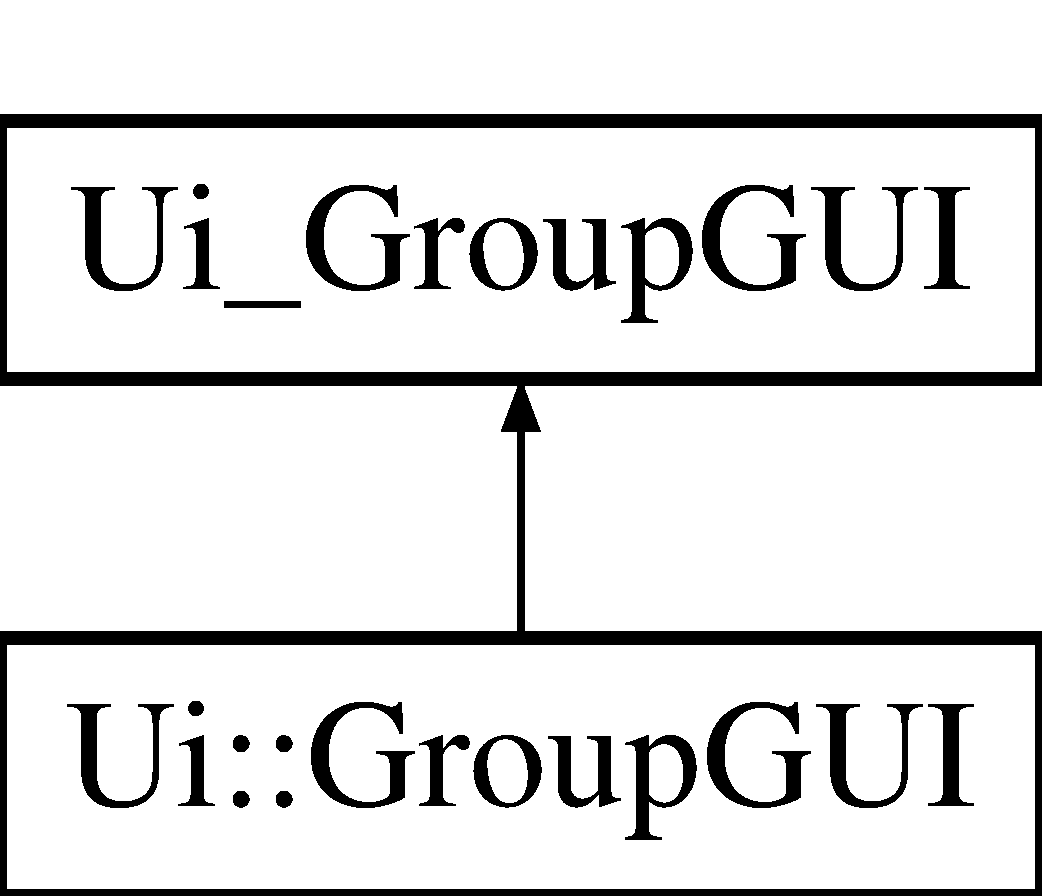
\includegraphics[height=2.000000cm]{classUi_1_1GroupGUI}
\end{center}
\end{figure}
\subsection*{Additional Inherited Members}


The documentation for this class was generated from the following file\+:\begin{DoxyCompactItemize}
\item 
/\+Users/\+Huy\+Nguyen/\+Desktop/\+School/\+C\+S 205/avengers/gui/ui\+\_\+groupgui.\+h\end{DoxyCompactItemize}

\hypertarget{classGroupMemberDB}{}\section{Group\+Member\+DB Class Reference}
\label{classGroupMemberDB}\index{Group\+Member\+DB@{Group\+Member\+DB}}


The \hyperlink{classGroupMemberDB}{Group\+Member\+DB} class.  




{\ttfamily \#include $<$groupmemberdb.\+h$>$}

\subsection*{Public Member Functions}
\begin{DoxyCompactItemize}
\item 
\hyperlink{classGroupMemberDB_a2b723703e4b30c4876fb02b62813a88a}{Group\+Member\+DB} ()\hypertarget{classGroupMemberDB_a2b723703e4b30c4876fb02b62813a88a}{}\label{classGroupMemberDB_a2b723703e4b30c4876fb02b62813a88a}

\begin{DoxyCompactList}\small\item\em \hyperlink{classGroupMemberDB}{Group\+Member\+DB} Construct a group member database. \end{DoxyCompactList}\item 
\hyperlink{classGroupMemberDB_a16cbd098d20e4ef4e848eb32ada8285c}{Group\+Member\+DB} (const Q\+String \&path)
\begin{DoxyCompactList}\small\item\em \hyperlink{classGroupMemberDB}{Group\+Member\+DB} Construct a group members database, given the path and the name of the database. \end{DoxyCompactList}\item 
\hyperlink{classGroupMemberDB_a0b0f153543aea1c695904b480f32ae11}{Group\+Member\+DB} (const Q\+String \&path, const Q\+String \&connection\+Name)
\begin{DoxyCompactList}\small\item\em \hyperlink{classGroupMemberDB}{Group\+Member\+DB}. \end{DoxyCompactList}\item 
\hyperlink{classGroupMemberDB_a10069210b5ed6856d20fb68192e28c52}{$\sim$\+Group\+Member\+DB} ()
\begin{DoxyCompactList}\small\item\em $\sim$\+Group\+Member\+DB \end{DoxyCompactList}\item 
bool \hyperlink{classGroupMemberDB_a1ae935d7a185d05e0f2eec85ec88e4bb}{is\+Open} () const 
\begin{DoxyCompactList}\small\item\em is\+Open \end{DoxyCompactList}\item 
bool \hyperlink{classGroupMemberDB_a23e976a5f1a2f7163c8c81cb5369e45f}{create\+Group} (int group\+ID, int account\+ID)
\begin{DoxyCompactList}\small\item\em create\+Group Create a new group with only one member in which the member is an admin. \end{DoxyCompactList}\item 
bool \hyperlink{classGroupMemberDB_a2027f8341b63928fd65f2791b18aa5a8}{add\+Group\+Member} (int group\+ID, int account\+ID, int group\+Admin\+Rights=0)
\begin{DoxyCompactList}\small\item\em add\+Group\+Member Adds a new group\+Membership by entering two entires into the group\+Member table\+: entry 1\+: user\+Id and group\+Member\+Id entry 2\+: group\+Member Id and User Id \end{DoxyCompactList}\item 
bool \hyperlink{classGroupMemberDB_af486022344b536264a49ae393420ad31}{group\+Member\+Exists} (int group\+ID, int account\+ID) const 
\begin{DoxyCompactList}\small\item\em group\+Membership\+Exists Check if group\+Membership exists, knowing the username \end{DoxyCompactList}\item 
bool \hyperlink{classGroupMemberDB_a527709d6b0a85ab6d452f56ff04903b8}{remove\+Group\+Member} (int group\+ID, int account\+ID)
\begin{DoxyCompactList}\small\item\em remove\+Group\+Member Remove a group\+Membership \end{DoxyCompactList}\item 
std\+::vector$<$ Group\+Member\+Info\+Type $>$ \hyperlink{classGroupMemberDB_ad926d57d28dfacd2fcde5511cae62f2e}{retrieve\+All\+Group\+Members\+Info} (int group\+ID)
\begin{DoxyCompactList}\small\item\em retrieve\+All\+Group\+Members\+Info Retrieve all group members from one group \end{DoxyCompactList}\item 
std\+::vector$<$ int $>$ \hyperlink{classGroupMemberDB_a43fa2ec7bc3c7e33970d60f480313974}{retrieve\+Group\+List} (int account\+ID)
\begin{DoxyCompactList}\small\item\em retrieve\+Group\+List Retrieve the group list in one account \end{DoxyCompactList}\item 
bool \hyperlink{classGroupMemberDB_a53061a946cb3b711a2e741c091421eec}{remove\+All\+Group\+Members} ()
\begin{DoxyCompactList}\small\item\em remove\+All\+Group\+Members Remove all group\+Members from the database \end{DoxyCompactList}\item 
int \hyperlink{classGroupMemberDB_a92446b1ca15758048fb48e17dff86d88}{get\+Max\+Group\+ID} ()
\begin{DoxyCompactList}\small\item\em get\+Max\+Group\+ID Retrieve the last group ID \end{DoxyCompactList}\item 
bool \hyperlink{classGroupMemberDB_aa89464f493771ef0cc0d661d4c7391b9}{set\+Admin} (int group\+ID, int account\+ID)
\begin{DoxyCompactList}\small\item\em set\+Admin Set a group member to become admin \end{DoxyCompactList}\end{DoxyCompactItemize}


\subsection{Detailed Description}
The \hyperlink{classGroupMemberDB}{Group\+Member\+DB} class. 

Insert/\+Delete from a sqlite3 table Group\+Members Column 1\+: Group\+ID I\+N\+T\+E\+G\+ER N\+OT N\+U\+LL Column 2\+: Friend\+ID I\+N\+T\+E\+G\+ER N\+OT N\+U\+LL Column 3\+: Group\+Admin\+Rights I\+N\+T\+E\+G\+ER N\+OT N\+U\+LL 

\subsection{Constructor \& Destructor Documentation}
\index{Group\+Member\+DB@{Group\+Member\+DB}!Group\+Member\+DB@{Group\+Member\+DB}}
\index{Group\+Member\+DB@{Group\+Member\+DB}!Group\+Member\+DB@{Group\+Member\+DB}}
\subsubsection[{\texorpdfstring{Group\+Member\+D\+B(const Q\+String \&path)}{GroupMemberDB(const QString &path)}}]{\setlength{\rightskip}{0pt plus 5cm}Group\+Member\+D\+B\+::\+Group\+Member\+DB (
\begin{DoxyParamCaption}
\item[{const Q\+String \&}]{path}
\end{DoxyParamCaption}
)}\hypertarget{classGroupMemberDB_a16cbd098d20e4ef4e848eb32ada8285c}{}\label{classGroupMemberDB_a16cbd098d20e4ef4e848eb32ada8285c}


\hyperlink{classGroupMemberDB}{Group\+Member\+DB} Construct a group members database, given the path and the name of the database. 


\begin{DoxyParams}{Parameters}
{\em path} & full path name of the group\+Memberdb \\
\hline
\end{DoxyParams}
\index{Group\+Member\+DB@{Group\+Member\+DB}!Group\+Member\+DB@{Group\+Member\+DB}}
\index{Group\+Member\+DB@{Group\+Member\+DB}!Group\+Member\+DB@{Group\+Member\+DB}}
\subsubsection[{\texorpdfstring{Group\+Member\+D\+B(const Q\+String \&path, const Q\+String \&connection\+Name)}{GroupMemberDB(const QString &path, const QString &connectionName)}}]{\setlength{\rightskip}{0pt plus 5cm}Group\+Member\+D\+B\+::\+Group\+Member\+DB (
\begin{DoxyParamCaption}
\item[{const Q\+String \&}]{path, }
\item[{const Q\+String \&}]{connection\+Name}
\end{DoxyParamCaption}
)}\hypertarget{classGroupMemberDB_a0b0f153543aea1c695904b480f32ae11}{}\label{classGroupMemberDB_a0b0f153543aea1c695904b480f32ae11}


\hyperlink{classGroupMemberDB}{Group\+Member\+DB}. 


\begin{DoxyParams}{Parameters}
{\em path} & \\
\hline
{\em connection\+Name} & \\
\hline
\end{DoxyParams}
\index{Group\+Member\+DB@{Group\+Member\+DB}!````~Group\+Member\+DB@{$\sim$\+Group\+Member\+DB}}
\index{````~Group\+Member\+DB@{$\sim$\+Group\+Member\+DB}!Group\+Member\+DB@{Group\+Member\+DB}}
\subsubsection[{\texorpdfstring{$\sim$\+Group\+Member\+D\+B()}{~GroupMemberDB()}}]{\setlength{\rightskip}{0pt plus 5cm}Group\+Member\+D\+B\+::$\sim$\+Group\+Member\+DB (
\begin{DoxyParamCaption}
{}
\end{DoxyParamCaption}
)}\hypertarget{classGroupMemberDB_a10069210b5ed6856d20fb68192e28c52}{}\label{classGroupMemberDB_a10069210b5ed6856d20fb68192e28c52}


$\sim$\+Group\+Member\+DB 

Default destructor for group\+Member database 

\subsection{Member Function Documentation}
\index{Group\+Member\+DB@{Group\+Member\+DB}!add\+Group\+Member@{add\+Group\+Member}}
\index{add\+Group\+Member@{add\+Group\+Member}!Group\+Member\+DB@{Group\+Member\+DB}}
\subsubsection[{\texorpdfstring{add\+Group\+Member(int group\+I\+D, int account\+I\+D, int group\+Admin\+Rights=0)}{addGroupMember(int groupID, int accountID, int groupAdminRights=0)}}]{\setlength{\rightskip}{0pt plus 5cm}bool Group\+Member\+D\+B\+::add\+Group\+Member (
\begin{DoxyParamCaption}
\item[{int}]{group\+ID, }
\item[{int}]{account\+ID, }
\item[{int}]{group\+Admin\+Rights = {\ttfamily 0}}
\end{DoxyParamCaption}
)}\hypertarget{classGroupMemberDB_a2027f8341b63928fd65f2791b18aa5a8}{}\label{classGroupMemberDB_a2027f8341b63928fd65f2791b18aa5a8}


add\+Group\+Member Adds a new group\+Membership by entering two entires into the group\+Member table\+: entry 1\+: user\+Id and group\+Member\+Id entry 2\+: group\+Member Id and User Id 


\begin{DoxyParams}{Parameters}
{\em group\+ID} & \hyperlink{classGroup}{Group} ID \\
\hline
{\em account\+ID} & Group\+Member ID \\
\hline
{\em group\+Admin\+Rights} & Whether the member is an admin, 0 if false, 1 if true. Default is 0 \\
\hline
\end{DoxyParams}
\begin{DoxyReturn}{Returns}
true if added, false if not added 
\end{DoxyReturn}
\index{Group\+Member\+DB@{Group\+Member\+DB}!create\+Group@{create\+Group}}
\index{create\+Group@{create\+Group}!Group\+Member\+DB@{Group\+Member\+DB}}
\subsubsection[{\texorpdfstring{create\+Group(int group\+I\+D, int account\+I\+D)}{createGroup(int groupID, int accountID)}}]{\setlength{\rightskip}{0pt plus 5cm}bool Group\+Member\+D\+B\+::create\+Group (
\begin{DoxyParamCaption}
\item[{int}]{group\+ID, }
\item[{int}]{account\+ID}
\end{DoxyParamCaption}
)}\hypertarget{classGroupMemberDB_a23e976a5f1a2f7163c8c81cb5369e45f}{}\label{classGroupMemberDB_a23e976a5f1a2f7163c8c81cb5369e45f}


create\+Group Create a new group with only one member in which the member is an admin. 


\begin{DoxyParams}{Parameters}
{\em group\+ID} & The ID of the group to be created \\
\hline
{\em account\+ID} & The ID of the account \\
\hline
\end{DoxyParams}
\begin{DoxyReturn}{Returns}
true if created, false if not 
\end{DoxyReturn}
\index{Group\+Member\+DB@{Group\+Member\+DB}!get\+Max\+Group\+ID@{get\+Max\+Group\+ID}}
\index{get\+Max\+Group\+ID@{get\+Max\+Group\+ID}!Group\+Member\+DB@{Group\+Member\+DB}}
\subsubsection[{\texorpdfstring{get\+Max\+Group\+I\+D()}{getMaxGroupID()}}]{\setlength{\rightskip}{0pt plus 5cm}int Group\+Member\+D\+B\+::get\+Max\+Group\+ID (
\begin{DoxyParamCaption}
{}
\end{DoxyParamCaption}
)}\hypertarget{classGroupMemberDB_a92446b1ca15758048fb48e17dff86d88}{}\label{classGroupMemberDB_a92446b1ca15758048fb48e17dff86d88}


get\+Max\+Group\+ID Retrieve the last group ID 

\begin{DoxyReturn}{Returns}
the max (last) group ID 
\end{DoxyReturn}
\index{Group\+Member\+DB@{Group\+Member\+DB}!group\+Member\+Exists@{group\+Member\+Exists}}
\index{group\+Member\+Exists@{group\+Member\+Exists}!Group\+Member\+DB@{Group\+Member\+DB}}
\subsubsection[{\texorpdfstring{group\+Member\+Exists(int group\+I\+D, int account\+I\+D) const }{groupMemberExists(int groupID, int accountID) const }}]{\setlength{\rightskip}{0pt plus 5cm}bool Group\+Member\+D\+B\+::group\+Member\+Exists (
\begin{DoxyParamCaption}
\item[{int}]{group\+ID, }
\item[{int}]{account\+ID}
\end{DoxyParamCaption}
) const}\hypertarget{classGroupMemberDB_af486022344b536264a49ae393420ad31}{}\label{classGroupMemberDB_af486022344b536264a49ae393420ad31}


group\+Membership\+Exists Check if group\+Membership exists, knowing the username 


\begin{DoxyParams}{Parameters}
{\em account\+ID} & User account ID \\
\hline
{\em group\+Member\+ID} & Group\+Member account ID \\
\hline
\end{DoxyParams}
\begin{DoxyReturn}{Returns}
true if yes, false if no 
\end{DoxyReturn}
\index{Group\+Member\+DB@{Group\+Member\+DB}!is\+Open@{is\+Open}}
\index{is\+Open@{is\+Open}!Group\+Member\+DB@{Group\+Member\+DB}}
\subsubsection[{\texorpdfstring{is\+Open() const }{isOpen() const }}]{\setlength{\rightskip}{0pt plus 5cm}bool Group\+Member\+D\+B\+::is\+Open (
\begin{DoxyParamCaption}
{}
\end{DoxyParamCaption}
) const}\hypertarget{classGroupMemberDB_a1ae935d7a185d05e0f2eec85ec88e4bb}{}\label{classGroupMemberDB_a1ae935d7a185d05e0f2eec85ec88e4bb}


is\+Open 

Check whether account database is open \begin{DoxyReturn}{Returns}
true if yes, false if no 
\end{DoxyReturn}
\index{Group\+Member\+DB@{Group\+Member\+DB}!remove\+All\+Group\+Members@{remove\+All\+Group\+Members}}
\index{remove\+All\+Group\+Members@{remove\+All\+Group\+Members}!Group\+Member\+DB@{Group\+Member\+DB}}
\subsubsection[{\texorpdfstring{remove\+All\+Group\+Members()}{removeAllGroupMembers()}}]{\setlength{\rightskip}{0pt plus 5cm}bool Group\+Member\+D\+B\+::remove\+All\+Group\+Members (
\begin{DoxyParamCaption}
{}
\end{DoxyParamCaption}
)}\hypertarget{classGroupMemberDB_a53061a946cb3b711a2e741c091421eec}{}\label{classGroupMemberDB_a53061a946cb3b711a2e741c091421eec}


remove\+All\+Group\+Members Remove all group\+Members from the database 

\begin{DoxyReturn}{Returns}
true if succeeded, false if failed 
\end{DoxyReturn}
\index{Group\+Member\+DB@{Group\+Member\+DB}!remove\+Group\+Member@{remove\+Group\+Member}}
\index{remove\+Group\+Member@{remove\+Group\+Member}!Group\+Member\+DB@{Group\+Member\+DB}}
\subsubsection[{\texorpdfstring{remove\+Group\+Member(int group\+I\+D, int account\+I\+D)}{removeGroupMember(int groupID, int accountID)}}]{\setlength{\rightskip}{0pt plus 5cm}bool Group\+Member\+D\+B\+::remove\+Group\+Member (
\begin{DoxyParamCaption}
\item[{int}]{group\+ID, }
\item[{int}]{account\+ID}
\end{DoxyParamCaption}
)}\hypertarget{classGroupMemberDB_a527709d6b0a85ab6d452f56ff04903b8}{}\label{classGroupMemberDB_a527709d6b0a85ab6d452f56ff04903b8}


remove\+Group\+Member Remove a group\+Membership 


\begin{DoxyParams}{Parameters}
{\em group\+ID} & The \hyperlink{classGroup}{Group} ID of the group in which a member got removed \\
\hline
{\em account\+ID} & The Account ID to be removed \\
\hline
\end{DoxyParams}
\begin{DoxyReturn}{Returns}
true if succeeded, false if failed 
\end{DoxyReturn}
\index{Group\+Member\+DB@{Group\+Member\+DB}!retrieve\+All\+Group\+Members\+Info@{retrieve\+All\+Group\+Members\+Info}}
\index{retrieve\+All\+Group\+Members\+Info@{retrieve\+All\+Group\+Members\+Info}!Group\+Member\+DB@{Group\+Member\+DB}}
\subsubsection[{\texorpdfstring{retrieve\+All\+Group\+Members\+Info(int group\+I\+D)}{retrieveAllGroupMembersInfo(int groupID)}}]{\setlength{\rightskip}{0pt plus 5cm}std\+::vector$<$ Group\+Member\+Info\+Type $>$ Group\+Member\+D\+B\+::retrieve\+All\+Group\+Members\+Info (
\begin{DoxyParamCaption}
\item[{int}]{group\+ID}
\end{DoxyParamCaption}
)}\hypertarget{classGroupMemberDB_ad926d57d28dfacd2fcde5511cae62f2e}{}\label{classGroupMemberDB_ad926d57d28dfacd2fcde5511cae62f2e}


retrieve\+All\+Group\+Members\+Info Retrieve all group members from one group 


\begin{DoxyParams}{Parameters}
{\em group\+ID} & The ID of the group \\
\hline
\end{DoxyParams}
\begin{DoxyReturn}{Returns}
a vector of all member info, including ID and the admin rights 
\end{DoxyReturn}
\index{Group\+Member\+DB@{Group\+Member\+DB}!retrieve\+Group\+List@{retrieve\+Group\+List}}
\index{retrieve\+Group\+List@{retrieve\+Group\+List}!Group\+Member\+DB@{Group\+Member\+DB}}
\subsubsection[{\texorpdfstring{retrieve\+Group\+List(int account\+I\+D)}{retrieveGroupList(int accountID)}}]{\setlength{\rightskip}{0pt plus 5cm}std\+::vector$<$ int $>$ Group\+Member\+D\+B\+::retrieve\+Group\+List (
\begin{DoxyParamCaption}
\item[{int}]{account\+ID}
\end{DoxyParamCaption}
)}\hypertarget{classGroupMemberDB_a43fa2ec7bc3c7e33970d60f480313974}{}\label{classGroupMemberDB_a43fa2ec7bc3c7e33970d60f480313974}


retrieve\+Group\+List Retrieve the group list in one account 


\begin{DoxyParams}{Parameters}
{\em account\+ID} & The ID of the account \\
\hline
\end{DoxyParams}
\begin{DoxyReturn}{Returns}
the list of group I\+Ds 
\end{DoxyReturn}
\index{Group\+Member\+DB@{Group\+Member\+DB}!set\+Admin@{set\+Admin}}
\index{set\+Admin@{set\+Admin}!Group\+Member\+DB@{Group\+Member\+DB}}
\subsubsection[{\texorpdfstring{set\+Admin(int group\+I\+D, int account\+I\+D)}{setAdmin(int groupID, int accountID)}}]{\setlength{\rightskip}{0pt plus 5cm}bool Group\+Member\+D\+B\+::set\+Admin (
\begin{DoxyParamCaption}
\item[{int}]{group\+ID, }
\item[{int}]{account\+ID}
\end{DoxyParamCaption}
)}\hypertarget{classGroupMemberDB_aa89464f493771ef0cc0d661d4c7391b9}{}\label{classGroupMemberDB_aa89464f493771ef0cc0d661d4c7391b9}


set\+Admin Set a group member to become admin 


\begin{DoxyParams}{Parameters}
{\em group\+ID} & \\
\hline
{\em account\+ID} & \\
\hline
\end{DoxyParams}
\begin{DoxyReturn}{Returns}
true if succeeded, false if failed 
\end{DoxyReturn}


The documentation for this class was generated from the following files\+:\begin{DoxyCompactItemize}
\item 
/\+Users/\+Huy\+Nguyen/\+Desktop/\+School/\+C\+S 205/avengers/database/groupmemberdb.\+h\item 
/\+Users/\+Huy\+Nguyen/\+Desktop/\+School/\+C\+S 205/avengers/database/groupmemberdb.\+cpp\end{DoxyCompactItemize}

\hypertarget{classGroupProfileGUI}{}\section{Group\+Profile\+G\+UI Class Reference}
\label{classGroupProfileGUI}\index{Group\+Profile\+G\+UI@{Group\+Profile\+G\+UI}}


The \hyperlink{classGroupProfileGUI}{Group\+Profile\+G\+UI} class provides a view for the group profile.  




{\ttfamily \#include $<$groupprofilegui.\+h$>$}

Inheritance diagram for Group\+Profile\+G\+UI\+:\begin{figure}[H]
\begin{center}
\leavevmode
\includegraphics[height=2.000000cm]{classGroupProfileGUI}
\end{center}
\end{figure}
\subsection*{Public Member Functions}
\begin{DoxyCompactItemize}
\item 
\hyperlink{classGroupProfileGUI_adf94380bfa993561c18c750d7522301c}{Group\+Profile\+G\+UI} (\hyperlink{classGroup}{Group} $\ast$group, Q\+Widget $\ast$parent=0)
\begin{DoxyCompactList}\small\item\em \hyperlink{classGroupProfileGUI}{Group\+Profile\+G\+UI} default constructor. \end{DoxyCompactList}\end{DoxyCompactItemize}


\subsection{Detailed Description}
The \hyperlink{classGroupProfileGUI}{Group\+Profile\+G\+UI} class provides a view for the group profile. 

\subsection{Constructor \& Destructor Documentation}
\index{Group\+Profile\+G\+UI@{Group\+Profile\+G\+UI}!Group\+Profile\+G\+UI@{Group\+Profile\+G\+UI}}
\index{Group\+Profile\+G\+UI@{Group\+Profile\+G\+UI}!Group\+Profile\+G\+UI@{Group\+Profile\+G\+UI}}
\subsubsection[{\texorpdfstring{Group\+Profile\+G\+U\+I(\+Group $\ast$group, Q\+Widget $\ast$parent=0)}{GroupProfileGUI(Group *group, QWidget *parent=0)}}]{\setlength{\rightskip}{0pt plus 5cm}Group\+Profile\+G\+U\+I\+::\+Group\+Profile\+G\+UI (
\begin{DoxyParamCaption}
\item[{{\bf Group} $\ast$}]{group, }
\item[{Q\+Widget $\ast$}]{parent = {\ttfamily 0}}
\end{DoxyParamCaption}
)\hspace{0.3cm}{\ttfamily [explicit]}}\hypertarget{classGroupProfileGUI_adf94380bfa993561c18c750d7522301c}{}\label{classGroupProfileGUI_adf94380bfa993561c18c750d7522301c}


\hyperlink{classGroupProfileGUI}{Group\+Profile\+G\+UI} default constructor. 


\begin{DoxyParams}{Parameters}
{\em group} & The group to be displayed \\
\hline
{\em parent} & \\
\hline
\end{DoxyParams}


The documentation for this class was generated from the following files\+:\begin{DoxyCompactItemize}
\item 
/\+Users/\+Huy\+Nguyen/\+Desktop/\+School/\+C\+S 205/avengers/gui/groupprofilegui.\+h\item 
/\+Users/\+Huy\+Nguyen/\+Desktop/\+School/\+C\+S 205/avengers/gui/groupprofilegui.\+cpp\end{DoxyCompactItemize}

\hypertarget{classUi_1_1GroupProfileGUI}{}\section{Ui\+:\+:Group\+Profile\+G\+UI Class Reference}
\label{classUi_1_1GroupProfileGUI}\index{Ui\+::\+Group\+Profile\+G\+UI@{Ui\+::\+Group\+Profile\+G\+UI}}
Inheritance diagram for Ui\+:\+:Group\+Profile\+G\+UI\+:\begin{figure}[H]
\begin{center}
\leavevmode
\includegraphics[height=2.000000cm]{classUi_1_1GroupProfileGUI}
\end{center}
\end{figure}
\subsection*{Additional Inherited Members}


The documentation for this class was generated from the following file\+:\begin{DoxyCompactItemize}
\item 
/\+Users/\+Huy\+Nguyen/\+Desktop/\+School/\+C\+S 205/avengers/gui/ui\+\_\+groupprofilegui.\+h\end{DoxyCompactItemize}

\hypertarget{classGroupScrapbookUI}{}\section{Group\+Scrapbook\+UI Class Reference}
\label{classGroupScrapbookUI}\index{Group\+Scrapbook\+UI@{Group\+Scrapbook\+UI}}


Groups \hyperlink{classScrapbook}{Scrapbook} UI handles all of the functions for group scrapbook in text UI.  




{\ttfamily \#include $<$groupscrapbookui.\+h$>$}

Inheritance diagram for Group\+Scrapbook\+UI\+:\begin{figure}[H]
\begin{center}
\leavevmode
\includegraphics[height=2.000000cm]{classGroupScrapbookUI}
\end{center}
\end{figure}
\subsection*{Public Member Functions}
\begin{DoxyCompactItemize}
\item 
\hyperlink{classGroupScrapbookUI_a48803a826aeb821546a02770b31e13bb}{Group\+Scrapbook\+UI} (Q\+String username, int group\+Id, \hyperlink{classGroup}{Group} $\ast$group, \hyperlink{classScrapbook}{Scrapbook} $\ast$group\+Scrapbook, Q\+String\+List friend\+Names)
\begin{DoxyCompactList}\small\item\em \hyperlink{classGroupScrapbookUI}{Group\+Scrapbook\+UI}. \end{DoxyCompactList}\item 
void \hyperlink{classGroupScrapbookUI_a3faeeff0a07f521520066f75a7f1b225}{draw\+Screen} (int v)
\begin{DoxyCompactList}\small\item\em Draw screen. \end{DoxyCompactList}\item 
void \hyperlink{classGroupScrapbookUI_afb2b9aae788b199fc621b7b11f208504}{take\+Command} (int selection)
\begin{DoxyCompactList}\small\item\em Take command Makes new screen based on user selection. \end{DoxyCompactList}\item 
void \hyperlink{classGroupScrapbookUI_abd2e2425a95a6251066f3ff14f335d27}{display\+Blog} (\hyperlink{classBlog}{Blog} $\ast$blog, int row)
\begin{DoxyCompactList}\small\item\em Display \hyperlink{classBlog}{Blog}. \end{DoxyCompactList}\item 
void \hyperlink{classGroupScrapbookUI_ac326e65f4fef7fefb7b0b5284e1653df}{display\+Tweet} (\hyperlink{classTweet}{Tweet} $\ast$tweet, int row)
\begin{DoxyCompactList}\small\item\em Display \hyperlink{classTweet}{Tweet}. \end{DoxyCompactList}\item 
void \hyperlink{classGroupScrapbookUI_a5195f5a6fbdd6cc8d90348f57322d36c}{view\+Blog} (int index)
\begin{DoxyCompactList}\small\item\em View \hyperlink{classBlog}{Blog} Displays selected blog on screen. \end{DoxyCompactList}\item 
int \hyperlink{classGroupScrapbookUI_ae9d46046637ad95dcc5cff4dd0a1cb37}{view\+Scrapbook} ()
\begin{DoxyCompactList}\small\item\em View \hyperlink{classScrapbook}{Scrapbook} Displays scrapbook posts on screen and allows user to scroll and select blogs to comment. \end{DoxyCompactList}\item 
void \hyperlink{classGroupScrapbookUI_ab9b96dbb884e49aa9a2146784340b0bf}{post\+Blog} ()\hypertarget{classGroupScrapbookUI_ab9b96dbb884e49aa9a2146784340b0bf}{}\label{classGroupScrapbookUI_ab9b96dbb884e49aa9a2146784340b0bf}

\begin{DoxyCompactList}\small\item\em \hyperlink{classPost}{Post} \hyperlink{classBlog}{Blog} Asks user for blog title and contents and creates blog post. \end{DoxyCompactList}\item 
void \hyperlink{classGroupScrapbookUI_a825bff1239eb5ee8062f0c3057e09af0}{post\+Comment} (int blog\+Index)
\begin{DoxyCompactList}\small\item\em \hyperlink{classPost}{Post} \hyperlink{classComment}{Comment} Adds comment to specific blog. \end{DoxyCompactList}\item 
void \hyperlink{classGroupScrapbookUI_a81992e0811cd86d11b9718e11b64db52}{post\+Tweet} ()\hypertarget{classGroupScrapbookUI_a81992e0811cd86d11b9718e11b64db52}{}\label{classGroupScrapbookUI_a81992e0811cd86d11b9718e11b64db52}

\begin{DoxyCompactList}\small\item\em \hyperlink{classPost}{Post} \hyperlink{classTweet}{Tweet} Asks user to enter text and creates tweet post. \end{DoxyCompactList}\item 
void \hyperlink{classGroupScrapbookUI_a389dda951ced6d3384cdb15bffb5e530}{add\+Friend} (int friend\+Index)
\begin{DoxyCompactList}\small\item\em Adds friend to group. \end{DoxyCompactList}\item 
int \hyperlink{classGroupScrapbookUI_a5f7c9c1a9ba8e3c4bcdac89762eca4a3}{select\+Friend} ()
\begin{DoxyCompactList}\small\item\em Displays friends on screen and allows user to select a friend. \end{DoxyCompactList}\item 
bool \hyperlink{classGroupScrapbookUI_a237840b9944b0589aa8d218fb03de420}{check\+Type} (int scrapbook\+Index)
\begin{DoxyCompactList}\small\item\em Checks post type. \end{DoxyCompactList}\end{DoxyCompactItemize}
\subsection*{Public Attributes}
\begin{DoxyCompactItemize}
\item 
int {\bfseries group\+Id}\hypertarget{classGroupScrapbookUI_a6d4cb2f6c2883e95e66489284512e535}{}\label{classGroupScrapbookUI_a6d4cb2f6c2883e95e66489284512e535}

\item 
\hyperlink{classGroup}{Group} $\ast$ {\bfseries group}\hypertarget{classGroupScrapbookUI_a00eef73a684700abf80579418c1ce3c2}{}\label{classGroupScrapbookUI_a00eef73a684700abf80579418c1ce3c2}

\item 
\hyperlink{classScrapbook}{Scrapbook} $\ast$ {\bfseries group\+Scrapbook}\hypertarget{classGroupScrapbookUI_a84517102b59705dc71a38c1d3bfccc7d}{}\label{classGroupScrapbookUI_a84517102b59705dc71a38c1d3bfccc7d}

\item 
Q\+String {\bfseries username}\hypertarget{classGroupScrapbookUI_a67fe7755854ad0efdf2062d7ced6ca5a}{}\label{classGroupScrapbookUI_a67fe7755854ad0efdf2062d7ced6ca5a}

\item 
Q\+String\+List {\bfseries friend\+Names}\hypertarget{classGroupScrapbookUI_a53d92693ac957d7e1ff8ee65402d3324}{}\label{classGroupScrapbookUI_a53d92693ac957d7e1ff8ee65402d3324}

\end{DoxyCompactItemize}


\subsection{Detailed Description}
Groups \hyperlink{classScrapbook}{Scrapbook} UI handles all of the functions for group scrapbook in text UI. 

\subsection{Constructor \& Destructor Documentation}
\index{Group\+Scrapbook\+UI@{Group\+Scrapbook\+UI}!Group\+Scrapbook\+UI@{Group\+Scrapbook\+UI}}
\index{Group\+Scrapbook\+UI@{Group\+Scrapbook\+UI}!Group\+Scrapbook\+UI@{Group\+Scrapbook\+UI}}
\subsubsection[{\texorpdfstring{Group\+Scrapbook\+U\+I(\+Q\+String username, int group\+Id, Group $\ast$group, Scrapbook $\ast$group\+Scrapbook, Q\+String\+List friend\+Names)}{GroupScrapbookUI(QString username, int groupId, Group *group, Scrapbook *groupScrapbook, QStringList friendNames)}}]{\setlength{\rightskip}{0pt plus 5cm}Group\+Scrapbook\+U\+I\+::\+Group\+Scrapbook\+UI (
\begin{DoxyParamCaption}
\item[{Q\+String}]{username, }
\item[{int}]{group\+Id, }
\item[{{\bf Group} $\ast$}]{group, }
\item[{{\bf Scrapbook} $\ast$}]{group\+Scrapbook, }
\item[{Q\+String\+List}]{friend\+Names}
\end{DoxyParamCaption}
)}\hypertarget{classGroupScrapbookUI_a48803a826aeb821546a02770b31e13bb}{}\label{classGroupScrapbookUI_a48803a826aeb821546a02770b31e13bb}


\hyperlink{classGroupScrapbookUI}{Group\+Scrapbook\+UI}. 


\begin{DoxyParams}{Parameters}
{\em username} & Username of current user \\
\hline
{\em group\+Id} & Id of indicated group \\
\hline
{\em group} & Indicated group \\
\hline
{\em group\+Scrapbook} & \hyperlink{classGroup}{Group}\textquotesingle{}s scrapbook \\
\hline
{\em friend\+Names} & List of user\textquotesingle{}s friends \\
\hline
\end{DoxyParams}


\subsection{Member Function Documentation}
\index{Group\+Scrapbook\+UI@{Group\+Scrapbook\+UI}!add\+Friend@{add\+Friend}}
\index{add\+Friend@{add\+Friend}!Group\+Scrapbook\+UI@{Group\+Scrapbook\+UI}}
\subsubsection[{\texorpdfstring{add\+Friend(int friend\+Index)}{addFriend(int friendIndex)}}]{\setlength{\rightskip}{0pt plus 5cm}void Group\+Scrapbook\+U\+I\+::add\+Friend (
\begin{DoxyParamCaption}
\item[{int}]{friend\+Index}
\end{DoxyParamCaption}
)}\hypertarget{classGroupScrapbookUI_a389dda951ced6d3384cdb15bffb5e530}{}\label{classGroupScrapbookUI_a389dda951ced6d3384cdb15bffb5e530}


Adds friend to group. 


\begin{DoxyParams}{Parameters}
{\em friend\+Index} & Position on friends list of selected friend \\
\hline
\end{DoxyParams}
\index{Group\+Scrapbook\+UI@{Group\+Scrapbook\+UI}!check\+Type@{check\+Type}}
\index{check\+Type@{check\+Type}!Group\+Scrapbook\+UI@{Group\+Scrapbook\+UI}}
\subsubsection[{\texorpdfstring{check\+Type(int scrapbook\+Index)}{checkType(int scrapbookIndex)}}]{\setlength{\rightskip}{0pt plus 5cm}bool Group\+Scrapbook\+U\+I\+::check\+Type (
\begin{DoxyParamCaption}
\item[{int}]{scrapbook\+Index}
\end{DoxyParamCaption}
)}\hypertarget{classGroupScrapbookUI_a237840b9944b0589aa8d218fb03de420}{}\label{classGroupScrapbookUI_a237840b9944b0589aa8d218fb03de420}


Checks post type. 


\begin{DoxyParams}{Parameters}
{\em scrapbook\+Index} & Index of post in post list \\
\hline
\end{DoxyParams}
\begin{DoxyReturn}{Returns}
True if post is a blog 
\end{DoxyReturn}
\index{Group\+Scrapbook\+UI@{Group\+Scrapbook\+UI}!display\+Blog@{display\+Blog}}
\index{display\+Blog@{display\+Blog}!Group\+Scrapbook\+UI@{Group\+Scrapbook\+UI}}
\subsubsection[{\texorpdfstring{display\+Blog(\+Blog $\ast$blog, int row)}{displayBlog(Blog *blog, int row)}}]{\setlength{\rightskip}{0pt plus 5cm}void Group\+Scrapbook\+U\+I\+::display\+Blog (
\begin{DoxyParamCaption}
\item[{{\bf Blog} $\ast$}]{blog, }
\item[{int}]{row}
\end{DoxyParamCaption}
)}\hypertarget{classGroupScrapbookUI_abd2e2425a95a6251066f3ff14f335d27}{}\label{classGroupScrapbookUI_abd2e2425a95a6251066f3ff14f335d27}


Display \hyperlink{classBlog}{Blog}. 


\begin{DoxyParams}{Parameters}
{\em \hyperlink{classBlog}{Blog}} & \hyperlink{classBlog}{Blog} to be displayed \\
\hline
{\em row} & Position on screen to display blog \\
\hline
\end{DoxyParams}
\index{Group\+Scrapbook\+UI@{Group\+Scrapbook\+UI}!display\+Tweet@{display\+Tweet}}
\index{display\+Tweet@{display\+Tweet}!Group\+Scrapbook\+UI@{Group\+Scrapbook\+UI}}
\subsubsection[{\texorpdfstring{display\+Tweet(\+Tweet $\ast$tweet, int row)}{displayTweet(Tweet *tweet, int row)}}]{\setlength{\rightskip}{0pt plus 5cm}void Group\+Scrapbook\+U\+I\+::display\+Tweet (
\begin{DoxyParamCaption}
\item[{{\bf Tweet} $\ast$}]{tweet, }
\item[{int}]{row}
\end{DoxyParamCaption}
)}\hypertarget{classGroupScrapbookUI_ac326e65f4fef7fefb7b0b5284e1653df}{}\label{classGroupScrapbookUI_ac326e65f4fef7fefb7b0b5284e1653df}


Display \hyperlink{classTweet}{Tweet}. 


\begin{DoxyParams}{Parameters}
{\em \hyperlink{classTweet}{Tweet}} & \hyperlink{classTweet}{Tweet} to be displayed \\
\hline
{\em row} & Position on screen to display tweet \\
\hline
\end{DoxyParams}
\index{Group\+Scrapbook\+UI@{Group\+Scrapbook\+UI}!draw\+Screen@{draw\+Screen}}
\index{draw\+Screen@{draw\+Screen}!Group\+Scrapbook\+UI@{Group\+Scrapbook\+UI}}
\subsubsection[{\texorpdfstring{draw\+Screen(int v)}{drawScreen(int v)}}]{\setlength{\rightskip}{0pt plus 5cm}void Group\+Scrapbook\+U\+I\+::draw\+Screen (
\begin{DoxyParamCaption}
\item[{int}]{v}
\end{DoxyParamCaption}
)\hspace{0.3cm}{\ttfamily [virtual]}}\hypertarget{classGroupScrapbookUI_a3faeeff0a07f521520066f75a7f1b225}{}\label{classGroupScrapbookUI_a3faeeff0a07f521520066f75a7f1b225}


Draw screen. 


\begin{DoxyParams}{Parameters}
{\em v} & Value of pointer \\
\hline
\end{DoxyParams}


Reimplemented from \hyperlink{classScreen_a7c48a93c2b9d4bdb92349e68d8f88c5e}{Screen}.

\index{Group\+Scrapbook\+UI@{Group\+Scrapbook\+UI}!post\+Comment@{post\+Comment}}
\index{post\+Comment@{post\+Comment}!Group\+Scrapbook\+UI@{Group\+Scrapbook\+UI}}
\subsubsection[{\texorpdfstring{post\+Comment(int blog\+Index)}{postComment(int blogIndex)}}]{\setlength{\rightskip}{0pt plus 5cm}void Group\+Scrapbook\+U\+I\+::post\+Comment (
\begin{DoxyParamCaption}
\item[{int}]{blog\+Index}
\end{DoxyParamCaption}
)}\hypertarget{classGroupScrapbookUI_a825bff1239eb5ee8062f0c3057e09af0}{}\label{classGroupScrapbookUI_a825bff1239eb5ee8062f0c3057e09af0}


\hyperlink{classPost}{Post} \hyperlink{classComment}{Comment} Adds comment to specific blog. 


\begin{DoxyParams}{Parameters}
{\em blog\+Index} & Index of blog \\
\hline
\end{DoxyParams}
\index{Group\+Scrapbook\+UI@{Group\+Scrapbook\+UI}!select\+Friend@{select\+Friend}}
\index{select\+Friend@{select\+Friend}!Group\+Scrapbook\+UI@{Group\+Scrapbook\+UI}}
\subsubsection[{\texorpdfstring{select\+Friend()}{selectFriend()}}]{\setlength{\rightskip}{0pt plus 5cm}int Group\+Scrapbook\+U\+I\+::select\+Friend (
\begin{DoxyParamCaption}
{}
\end{DoxyParamCaption}
)}\hypertarget{classGroupScrapbookUI_a5f7c9c1a9ba8e3c4bcdac89762eca4a3}{}\label{classGroupScrapbookUI_a5f7c9c1a9ba8e3c4bcdac89762eca4a3}


Displays friends on screen and allows user to select a friend. 

\begin{DoxyReturn}{Returns}
Index of selected friend 
\end{DoxyReturn}
\index{Group\+Scrapbook\+UI@{Group\+Scrapbook\+UI}!take\+Command@{take\+Command}}
\index{take\+Command@{take\+Command}!Group\+Scrapbook\+UI@{Group\+Scrapbook\+UI}}
\subsubsection[{\texorpdfstring{take\+Command(int selection)}{takeCommand(int selection)}}]{\setlength{\rightskip}{0pt plus 5cm}void Group\+Scrapbook\+U\+I\+::take\+Command (
\begin{DoxyParamCaption}
\item[{int}]{selection}
\end{DoxyParamCaption}
)}\hypertarget{classGroupScrapbookUI_afb2b9aae788b199fc621b7b11f208504}{}\label{classGroupScrapbookUI_afb2b9aae788b199fc621b7b11f208504}


Take command Makes new screen based on user selection. 


\begin{DoxyParams}{Parameters}
{\em selection} & Pointer value when enter is pressed \\
\hline
\end{DoxyParams}
\index{Group\+Scrapbook\+UI@{Group\+Scrapbook\+UI}!view\+Blog@{view\+Blog}}
\index{view\+Blog@{view\+Blog}!Group\+Scrapbook\+UI@{Group\+Scrapbook\+UI}}
\subsubsection[{\texorpdfstring{view\+Blog(int index)}{viewBlog(int index)}}]{\setlength{\rightskip}{0pt plus 5cm}void Group\+Scrapbook\+U\+I\+::view\+Blog (
\begin{DoxyParamCaption}
\item[{int}]{index}
\end{DoxyParamCaption}
)}\hypertarget{classGroupScrapbookUI_a5195f5a6fbdd6cc8d90348f57322d36c}{}\label{classGroupScrapbookUI_a5195f5a6fbdd6cc8d90348f57322d36c}


View \hyperlink{classBlog}{Blog} Displays selected blog on screen. 


\begin{DoxyParams}{Parameters}
{\em index} & Index of selected blog \\
\hline
\end{DoxyParams}
\index{Group\+Scrapbook\+UI@{Group\+Scrapbook\+UI}!view\+Scrapbook@{view\+Scrapbook}}
\index{view\+Scrapbook@{view\+Scrapbook}!Group\+Scrapbook\+UI@{Group\+Scrapbook\+UI}}
\subsubsection[{\texorpdfstring{view\+Scrapbook()}{viewScrapbook()}}]{\setlength{\rightskip}{0pt plus 5cm}int Group\+Scrapbook\+U\+I\+::view\+Scrapbook (
\begin{DoxyParamCaption}
{}
\end{DoxyParamCaption}
)}\hypertarget{classGroupScrapbookUI_ae9d46046637ad95dcc5cff4dd0a1cb37}{}\label{classGroupScrapbookUI_ae9d46046637ad95dcc5cff4dd0a1cb37}


View \hyperlink{classScrapbook}{Scrapbook} Displays scrapbook posts on screen and allows user to scroll and select blogs to comment. 

\begin{DoxyReturn}{Returns}
location of pointer on screen 
\end{DoxyReturn}


The documentation for this class was generated from the following files\+:\begin{DoxyCompactItemize}
\item 
/\+Users/\+Huy\+Nguyen/\+Desktop/\+School/\+C\+S 205/avengers/textui/groupscrapbookui.\+h\item 
/\+Users/\+Huy\+Nguyen/\+Desktop/\+School/\+C\+S 205/avengers/textui/groupscrapbookui.\+cpp\end{DoxyCompactItemize}

\hypertarget{classGroupsUI}{}\section{Groups\+UI Class Reference}
\label{classGroupsUI}\index{Groups\+UI@{Groups\+UI}}


The \hyperlink{classGroupsUI}{Groups\+UI} handles functionality for creating groups and editing group profiles in text UI.  




{\ttfamily \#include $<$groupsui.\+h$>$}

Inheritance diagram for Groups\+UI\+:\begin{figure}[H]
\begin{center}
\leavevmode
\includegraphics[height=2.000000cm]{classGroupsUI}
\end{center}
\end{figure}
\subsection*{Public Member Functions}
\begin{DoxyCompactItemize}
\item 
\hyperlink{classGroupsUI_a874193355176aa40b6fce30e8aeb708f}{Groups\+UI} (\hyperlink{classAccountController}{Account\+Controller} $\ast$account\+Control)
\begin{DoxyCompactList}\small\item\em \hyperlink{classGroupsUI}{Groups\+UI}. \end{DoxyCompactList}\item 
int \hyperlink{classGroupsUI_a2d1126b3e3cd8ecba3c0e1bebc521736}{select\+Group} ()\hypertarget{classGroupsUI_a2d1126b3e3cd8ecba3c0e1bebc521736}{}\label{classGroupsUI_a2d1126b3e3cd8ecba3c0e1bebc521736}

\begin{DoxyCompactList}\small\item\em Select \hyperlink{classGroup}{Group} Displays list of groups and allows user to select one to enter. \end{DoxyCompactList}\item 
void \hyperlink{classGroupsUI_ac2513b740609c8263db85b91cf69ac2b}{enter\+Group} (int index)
\begin{DoxyCompactList}\small\item\em Enter \hyperlink{classGroup}{Group} Enters selected group. \end{DoxyCompactList}\item 
void \hyperlink{classGroupsUI_a77de7dab3346d7e57fb389f396cb24a6}{view\+Profile} (int index)
\begin{DoxyCompactList}\small\item\em View \hyperlink{classProfile}{Profile} Views profile of selected group. \end{DoxyCompactList}\item 
void \hyperlink{classGroupsUI_a64cf522aeb035d00db3bbd8da38875bb}{take\+Command} (int selection)
\begin{DoxyCompactList}\small\item\em Take command Makes new screen based on user selection. \end{DoxyCompactList}\item 
void \hyperlink{classGroupsUI_ab3edbe00293aeda49e5251d2777984bf}{draw\+Screen} (int v)
\begin{DoxyCompactList}\small\item\em Draw screen. \end{DoxyCompactList}\item 
void \hyperlink{classGroupsUI_a4ce092af55dae46d5c270d5f32a69784}{create\+Group} ()\hypertarget{classGroupsUI_a4ce092af55dae46d5c270d5f32a69784}{}\label{classGroupsUI_a4ce092af55dae46d5c270d5f32a69784}

\begin{DoxyCompactList}\small\item\em Create \hyperlink{classGroup}{Group} Asks user to enter necessary information to create a group and creates group with indicated information. \end{DoxyCompactList}\end{DoxyCompactItemize}
\subsection*{Public Attributes}
\begin{DoxyCompactItemize}
\item 
\hyperlink{classGroupScrapbookUI}{Group\+Scrapbook\+UI} $\ast$ {\bfseries scrapbook}\hypertarget{classGroupsUI_ab0700dac6c6bf69b2c16811257c10296}{}\label{classGroupsUI_ab0700dac6c6bf69b2c16811257c10296}

\end{DoxyCompactItemize}


\subsection{Detailed Description}
The \hyperlink{classGroupsUI}{Groups\+UI} handles functionality for creating groups and editing group profiles in text UI. 

Users can also create a new \hyperlink{classGroupScrapbookUI}{Group\+Scrapbook\+UI} from this screen. 

\subsection{Constructor \& Destructor Documentation}
\index{Groups\+UI@{Groups\+UI}!Groups\+UI@{Groups\+UI}}
\index{Groups\+UI@{Groups\+UI}!Groups\+UI@{Groups\+UI}}
\subsubsection[{\texorpdfstring{Groups\+U\+I(\+Account\+Controller $\ast$account\+Control)}{GroupsUI(AccountController *accountControl)}}]{\setlength{\rightskip}{0pt plus 5cm}Groups\+U\+I\+::\+Groups\+UI (
\begin{DoxyParamCaption}
\item[{{\bf Account\+Controller} $\ast$}]{account\+Control}
\end{DoxyParamCaption}
)}\hypertarget{classGroupsUI_a874193355176aa40b6fce30e8aeb708f}{}\label{classGroupsUI_a874193355176aa40b6fce30e8aeb708f}


\hyperlink{classGroupsUI}{Groups\+UI}. 


\begin{DoxyParams}{Parameters}
{\em account\+Control} & Account Controller \\
\hline
\end{DoxyParams}


\subsection{Member Function Documentation}
\index{Groups\+UI@{Groups\+UI}!draw\+Screen@{draw\+Screen}}
\index{draw\+Screen@{draw\+Screen}!Groups\+UI@{Groups\+UI}}
\subsubsection[{\texorpdfstring{draw\+Screen(int v)}{drawScreen(int v)}}]{\setlength{\rightskip}{0pt plus 5cm}void Groups\+U\+I\+::draw\+Screen (
\begin{DoxyParamCaption}
\item[{int}]{v}
\end{DoxyParamCaption}
)\hspace{0.3cm}{\ttfamily [virtual]}}\hypertarget{classGroupsUI_ab3edbe00293aeda49e5251d2777984bf}{}\label{classGroupsUI_ab3edbe00293aeda49e5251d2777984bf}


Draw screen. 


\begin{DoxyParams}{Parameters}
{\em v} & Value of pointer \\
\hline
\end{DoxyParams}


Reimplemented from \hyperlink{classScreen_a7c48a93c2b9d4bdb92349e68d8f88c5e}{Screen}.

\index{Groups\+UI@{Groups\+UI}!enter\+Group@{enter\+Group}}
\index{enter\+Group@{enter\+Group}!Groups\+UI@{Groups\+UI}}
\subsubsection[{\texorpdfstring{enter\+Group(int index)}{enterGroup(int index)}}]{\setlength{\rightskip}{0pt plus 5cm}void Groups\+U\+I\+::enter\+Group (
\begin{DoxyParamCaption}
\item[{int}]{index}
\end{DoxyParamCaption}
)}\hypertarget{classGroupsUI_ac2513b740609c8263db85b91cf69ac2b}{}\label{classGroupsUI_ac2513b740609c8263db85b91cf69ac2b}


Enter \hyperlink{classGroup}{Group} Enters selected group. 


\begin{DoxyParams}{Parameters}
{\em index} & Index of selected group on group list \\
\hline
\end{DoxyParams}
\index{Groups\+UI@{Groups\+UI}!take\+Command@{take\+Command}}
\index{take\+Command@{take\+Command}!Groups\+UI@{Groups\+UI}}
\subsubsection[{\texorpdfstring{take\+Command(int selection)}{takeCommand(int selection)}}]{\setlength{\rightskip}{0pt plus 5cm}void Groups\+U\+I\+::take\+Command (
\begin{DoxyParamCaption}
\item[{int}]{selection}
\end{DoxyParamCaption}
)}\hypertarget{classGroupsUI_a64cf522aeb035d00db3bbd8da38875bb}{}\label{classGroupsUI_a64cf522aeb035d00db3bbd8da38875bb}


Take command Makes new screen based on user selection. 


\begin{DoxyParams}{Parameters}
{\em selection} & Pointer value when enter is pressed \\
\hline
\end{DoxyParams}
\index{Groups\+UI@{Groups\+UI}!view\+Profile@{view\+Profile}}
\index{view\+Profile@{view\+Profile}!Groups\+UI@{Groups\+UI}}
\subsubsection[{\texorpdfstring{view\+Profile(int index)}{viewProfile(int index)}}]{\setlength{\rightskip}{0pt plus 5cm}void Groups\+U\+I\+::view\+Profile (
\begin{DoxyParamCaption}
\item[{int}]{index}
\end{DoxyParamCaption}
)}\hypertarget{classGroupsUI_a77de7dab3346d7e57fb389f396cb24a6}{}\label{classGroupsUI_a77de7dab3346d7e57fb389f396cb24a6}


View \hyperlink{classProfile}{Profile} Views profile of selected group. 


\begin{DoxyParams}{Parameters}
{\em index} & Index of selected group on group list \\
\hline
\end{DoxyParams}


The documentation for this class was generated from the following files\+:\begin{DoxyCompactItemize}
\item 
/\+Users/\+Huy\+Nguyen/\+Desktop/\+School/\+C\+S 205/avengers/textui/groupsui.\+h\item 
/\+Users/\+Huy\+Nguyen/\+Desktop/\+School/\+C\+S 205/avengers/textui/groupsui.\+cpp\end{DoxyCompactItemize}

\hypertarget{classLoginGUI}{}\section{Login\+G\+UI Class Reference}
\label{classLoginGUI}\index{Login\+G\+UI@{Login\+G\+UI}}


The \hyperlink{classLoginGUI}{Login\+G\+UI} class provides the functionality to login to the application.  




{\ttfamily \#include $<$logingui.\+h$>$}

Inheritance diagram for Login\+G\+UI\+:\begin{figure}[H]
\begin{center}
\leavevmode
\includegraphics[height=2.000000cm]{classLoginGUI}
\end{center}
\end{figure}
\subsection*{Public Member Functions}
\begin{DoxyCompactItemize}
\item 
\hyperlink{classLoginGUI_a463b5504797bf4189053649348314787}{Login\+G\+UI} (\hyperlink{classAccountController}{Account\+Controller} $\ast$input\+Account\+Controller, Q\+Widget $\ast$parent=0)
\begin{DoxyCompactList}\small\item\em \hyperlink{classLoginGUI}{Login\+G\+UI} constructs a login window. \end{DoxyCompactList}\item 
void \hyperlink{classLoginGUI_a25e4f8144c8d24f7f0431828e09d61f3}{set\+Main\+Window} (\hyperlink{classMainWindow}{Main\+Window} $\ast$input)
\begin{DoxyCompactList}\small\item\em set\+Main\+Window sets the main window in the class \end{DoxyCompactList}\item 
void \hyperlink{classLoginGUI_aed7e048a3e518a89a5cbc508df88831e}{set\+Create\+Account\+View} (\hyperlink{classCreateAccountGUI}{Create\+Account\+G\+UI} $\ast$input)
\begin{DoxyCompactList}\small\item\em set\+Create\+Account\+View sets the create account window \end{DoxyCompactList}\item 
void \hyperlink{classLoginGUI_ac35e63981f4d570fa9fb528393a8db1e}{clear\+All\+Fields} ()\hypertarget{classLoginGUI_ac35e63981f4d570fa9fb528393a8db1e}{}\label{classLoginGUI_ac35e63981f4d570fa9fb528393a8db1e}

\begin{DoxyCompactList}\small\item\em clear\+All\+Fields Clears all fields in the Login UI \end{DoxyCompactList}\item 
bool \hyperlink{classLoginGUI_a675a9105543ff0df4ae588c9c3060cf8}{login} ()\hypertarget{classLoginGUI_a675a9105543ff0df4ae588c9c3060cf8}{}\label{classLoginGUI_a675a9105543ff0df4ae588c9c3060cf8}

\begin{DoxyCompactList}\small\item\em login Login to the account \end{DoxyCompactList}\end{DoxyCompactItemize}
\subsection*{Static Public Member Functions}
\begin{DoxyCompactItemize}
\item 
static bool \hyperlink{classLoginGUI_a9c4874e6e42919bbf5c0ea09a892ca5d}{is\+Finished} ()
\begin{DoxyCompactList}\small\item\em is\+Finished When the \hyperlink{classLoginUI}{Login\+UI} can be closed \end{DoxyCompactList}\end{DoxyCompactItemize}


\subsection{Detailed Description}
The \hyperlink{classLoginGUI}{Login\+G\+UI} class provides the functionality to login to the application. 

\subsection{Constructor \& Destructor Documentation}
\index{Login\+G\+UI@{Login\+G\+UI}!Login\+G\+UI@{Login\+G\+UI}}
\index{Login\+G\+UI@{Login\+G\+UI}!Login\+G\+UI@{Login\+G\+UI}}
\subsubsection[{\texorpdfstring{Login\+G\+U\+I(\+Account\+Controller $\ast$input\+Account\+Controller, Q\+Widget $\ast$parent=0)}{LoginGUI(AccountController *inputAccountController, QWidget *parent=0)}}]{\setlength{\rightskip}{0pt plus 5cm}Login\+G\+U\+I\+::\+Login\+G\+UI (
\begin{DoxyParamCaption}
\item[{{\bf Account\+Controller} $\ast$}]{input\+Account\+Controller, }
\item[{Q\+Widget $\ast$}]{parent = {\ttfamily 0}}
\end{DoxyParamCaption}
)\hspace{0.3cm}{\ttfamily [explicit]}}\hypertarget{classLoginGUI_a463b5504797bf4189053649348314787}{}\label{classLoginGUI_a463b5504797bf4189053649348314787}


\hyperlink{classLoginGUI}{Login\+G\+UI} constructs a login window. 


\begin{DoxyParams}{Parameters}
{\em input\+Account\+Controller} & The model \\
\hline
{\em parent} & \\
\hline
\end{DoxyParams}


\subsection{Member Function Documentation}
\index{Login\+G\+UI@{Login\+G\+UI}!is\+Finished@{is\+Finished}}
\index{is\+Finished@{is\+Finished}!Login\+G\+UI@{Login\+G\+UI}}
\subsubsection[{\texorpdfstring{is\+Finished()}{isFinished()}}]{\setlength{\rightskip}{0pt plus 5cm}static bool Login\+G\+U\+I\+::is\+Finished (
\begin{DoxyParamCaption}
{}
\end{DoxyParamCaption}
)\hspace{0.3cm}{\ttfamily [inline]}, {\ttfamily [static]}}\hypertarget{classLoginGUI_a9c4874e6e42919bbf5c0ea09a892ca5d}{}\label{classLoginGUI_a9c4874e6e42919bbf5c0ea09a892ca5d}


is\+Finished When the \hyperlink{classLoginUI}{Login\+UI} can be closed 

\begin{DoxyReturn}{Returns}

\end{DoxyReturn}
\index{Login\+G\+UI@{Login\+G\+UI}!set\+Create\+Account\+View@{set\+Create\+Account\+View}}
\index{set\+Create\+Account\+View@{set\+Create\+Account\+View}!Login\+G\+UI@{Login\+G\+UI}}
\subsubsection[{\texorpdfstring{set\+Create\+Account\+View(\+Create\+Account\+G\+U\+I $\ast$input)}{setCreateAccountView(CreateAccountGUI *input)}}]{\setlength{\rightskip}{0pt plus 5cm}void Login\+G\+U\+I\+::set\+Create\+Account\+View (
\begin{DoxyParamCaption}
\item[{{\bf Create\+Account\+G\+UI} $\ast$}]{input}
\end{DoxyParamCaption}
)\hspace{0.3cm}{\ttfamily [inline]}}\hypertarget{classLoginGUI_aed7e048a3e518a89a5cbc508df88831e}{}\label{classLoginGUI_aed7e048a3e518a89a5cbc508df88831e}


set\+Create\+Account\+View sets the create account window 


\begin{DoxyParams}{Parameters}
{\em input} & the Create Account window \\
\hline
\end{DoxyParams}
\index{Login\+G\+UI@{Login\+G\+UI}!set\+Main\+Window@{set\+Main\+Window}}
\index{set\+Main\+Window@{set\+Main\+Window}!Login\+G\+UI@{Login\+G\+UI}}
\subsubsection[{\texorpdfstring{set\+Main\+Window(\+Main\+Window $\ast$input)}{setMainWindow(MainWindow *input)}}]{\setlength{\rightskip}{0pt plus 5cm}void Login\+G\+U\+I\+::set\+Main\+Window (
\begin{DoxyParamCaption}
\item[{{\bf Main\+Window} $\ast$}]{input}
\end{DoxyParamCaption}
)\hspace{0.3cm}{\ttfamily [inline]}}\hypertarget{classLoginGUI_a25e4f8144c8d24f7f0431828e09d61f3}{}\label{classLoginGUI_a25e4f8144c8d24f7f0431828e09d61f3}


set\+Main\+Window sets the main window in the class 


\begin{DoxyParams}{Parameters}
{\em input} & the main window \\
\hline
\end{DoxyParams}


The documentation for this class was generated from the following files\+:\begin{DoxyCompactItemize}
\item 
/\+Users/\+Huy\+Nguyen/\+Desktop/\+School/\+C\+S 205/avengers/gui/logingui.\+h\item 
/\+Users/\+Huy\+Nguyen/\+Desktop/\+School/\+C\+S 205/avengers/gui/logingui.\+cpp\end{DoxyCompactItemize}

\hypertarget{classUi_1_1LoginGUI}{}\section{Ui\+:\+:Login\+G\+UI Class Reference}
\label{classUi_1_1LoginGUI}\index{Ui\+::\+Login\+G\+UI@{Ui\+::\+Login\+G\+UI}}
Inheritance diagram for Ui\+:\+:Login\+G\+UI\+:\begin{figure}[H]
\begin{center}
\leavevmode
\includegraphics[height=2.000000cm]{classUi_1_1LoginGUI}
\end{center}
\end{figure}
\subsection*{Additional Inherited Members}


The documentation for this class was generated from the following file\+:\begin{DoxyCompactItemize}
\item 
/\+Users/\+Huy\+Nguyen/\+Desktop/\+School/\+C\+S 205/avengers/gui/ui\+\_\+logingui.\+h\end{DoxyCompactItemize}

\hypertarget{classLoginUI}{}\section{Login\+UI Class Reference}
\label{classLoginUI}\index{Login\+UI@{Login\+UI}}


Login \hyperlink{classScreen}{Screen}.  




{\ttfamily \#include $<$loginui.\+h$>$}

Inheritance diagram for Login\+UI\+:\begin{figure}[H]
\begin{center}
\leavevmode
\includegraphics[height=2.000000cm]{classLoginUI}
\end{center}
\end{figure}
\subsection*{Public Member Functions}
\begin{DoxyCompactItemize}
\item 
\hyperlink{classLoginUI_a499c91383c83dac9929fd0f855bd7ce4}{Login\+UI} (\hyperlink{classAccountController}{Account\+Controller} $\ast$account\+Control)
\begin{DoxyCompactList}\small\item\em \hyperlink{classLoginUI}{Login\+UI}. \end{DoxyCompactList}\item 
void \hyperlink{classLoginUI_a118ca727f08f4430d0b7e8ae15c521dd}{run} ()
\begin{DoxyCompactList}\small\item\em run Asks user for username and password. \end{DoxyCompactList}\end{DoxyCompactItemize}
\subsection*{Public Attributes}
\begin{DoxyCompactItemize}
\item 
\hyperlink{classMainMenu}{Main\+Menu} $\ast$ {\bfseries menu}\hypertarget{classLoginUI_a46b43e48521a28e8aff9c867459aee43}{}\label{classLoginUI_a46b43e48521a28e8aff9c867459aee43}

\end{DoxyCompactItemize}


\subsection{Detailed Description}
Login \hyperlink{classScreen}{Screen}. 

Asks user for username and password. Creates main menu of password is correct for entered username 

\subsection{Constructor \& Destructor Documentation}
\index{Login\+UI@{Login\+UI}!Login\+UI@{Login\+UI}}
\index{Login\+UI@{Login\+UI}!Login\+UI@{Login\+UI}}
\subsubsection[{\texorpdfstring{Login\+U\+I(\+Account\+Controller $\ast$account\+Control)}{LoginUI(AccountController *accountControl)}}]{\setlength{\rightskip}{0pt plus 5cm}Login\+U\+I\+::\+Login\+UI (
\begin{DoxyParamCaption}
\item[{{\bf Account\+Controller} $\ast$}]{account\+Control}
\end{DoxyParamCaption}
)}\hypertarget{classLoginUI_a499c91383c83dac9929fd0f855bd7ce4}{}\label{classLoginUI_a499c91383c83dac9929fd0f855bd7ce4}


\hyperlink{classLoginUI}{Login\+UI}. 


\begin{DoxyParams}{Parameters}
{\em account\+Controller} & Account Controller \\
\hline
\end{DoxyParams}


\subsection{Member Function Documentation}
\index{Login\+UI@{Login\+UI}!run@{run}}
\index{run@{run}!Login\+UI@{Login\+UI}}
\subsubsection[{\texorpdfstring{run()}{run()}}]{\setlength{\rightskip}{0pt plus 5cm}void Login\+U\+I\+::run (
\begin{DoxyParamCaption}
{}
\end{DoxyParamCaption}
)}\hypertarget{classLoginUI_a118ca727f08f4430d0b7e8ae15c521dd}{}\label{classLoginUI_a118ca727f08f4430d0b7e8ae15c521dd}


run Asks user for username and password. 

Creates main menu of password is correct for entered username 

The documentation for this class was generated from the following files\+:\begin{DoxyCompactItemize}
\item 
/\+Users/\+Huy\+Nguyen/\+Desktop/\+School/\+C\+S 205/avengers/textui/loginui.\+h\item 
/\+Users/\+Huy\+Nguyen/\+Desktop/\+School/\+C\+S 205/avengers/textui/loginui.\+cpp\end{DoxyCompactItemize}

\hypertarget{classMainMenu}{}\section{Main\+Menu Class Reference}
\label{classMainMenu}\index{Main\+Menu@{Main\+Menu}}


The Main Menu Prompts the to select one of several different actions.  




{\ttfamily \#include $<$mainmenu.\+h$>$}

Inheritance diagram for Main\+Menu\+:\begin{figure}[H]
\begin{center}
\leavevmode
\includegraphics[height=2.000000cm]{classMainMenu}
\end{center}
\end{figure}
\subsection*{Public Member Functions}
\begin{DoxyCompactItemize}
\item 
\hyperlink{classMainMenu_a59fd6b4194b456791c0f17d223e37bea}{Main\+Menu} (\hyperlink{classAccountController}{Account\+Controller} $\ast$account\+Control)
\begin{DoxyCompactList}\small\item\em \hyperlink{classMainMenu}{Main\+Menu} Displays Main Menu. \end{DoxyCompactList}\item 
\hyperlink{classMainMenu_a0a19ddba3ac52bf39c09b579171c98f2}{$\sim$\+Main\+Menu} ()\hypertarget{classMainMenu_a0a19ddba3ac52bf39c09b579171c98f2}{}\label{classMainMenu_a0a19ddba3ac52bf39c09b579171c98f2}

\begin{DoxyCompactList}\small\item\em $\sim$\+Main\+Menu \end{DoxyCompactList}\item 
void \hyperlink{classMainMenu_ae86dc04cf1ae13a6041ffbd7212e5421}{draw\+Screen} (int v)
\begin{DoxyCompactList}\small\item\em Draw screen. \end{DoxyCompactList}\item 
void \hyperlink{classMainMenu_ab91c57315336821b94bd1240550183a4}{change\+Screen} (int selection)
\begin{DoxyCompactList}\small\item\em Change \hyperlink{classScreen}{Screen} Makes new screen based on user selection. \end{DoxyCompactList}\end{DoxyCompactItemize}
\subsection*{Public Attributes}
\begin{DoxyCompactItemize}
\item 
\hyperlink{classFriendsUI}{Friends\+UI} $\ast$ {\bfseries friends}\hypertarget{classMainMenu_ac05fadacf74b5741d0b8ce500596bae3}{}\label{classMainMenu_ac05fadacf74b5741d0b8ce500596bae3}

\item 
\hyperlink{classChatUI}{Chat\+UI} $\ast$ {\bfseries chats}\hypertarget{classMainMenu_a5cdb3f46d4d1caba34a2fa78bf90229c}{}\label{classMainMenu_a5cdb3f46d4d1caba34a2fa78bf90229c}

\item 
\hyperlink{classScrapbookUI}{Scrapbook\+UI} $\ast$ {\bfseries scrapbook}\hypertarget{classMainMenu_a83d3d33ace5e26e52965648514f14f41}{}\label{classMainMenu_a83d3d33ace5e26e52965648514f14f41}

\item 
\hyperlink{classProfileUI}{Profile\+UI} $\ast$ {\bfseries profile}\hypertarget{classMainMenu_adcd9f278a7861cc7cc8db31ea8db804b}{}\label{classMainMenu_adcd9f278a7861cc7cc8db31ea8db804b}

\item 
\hyperlink{classFeedUI}{Feed\+UI} $\ast$ {\bfseries feed}\hypertarget{classMainMenu_a9347d630d6a161d91d822f00e6542859}{}\label{classMainMenu_a9347d630d6a161d91d822f00e6542859}

\item 
\hyperlink{classGroupsUI}{Groups\+UI} $\ast$ {\bfseries groups}\hypertarget{classMainMenu_a11b7a11b936f917358f5c44f177f3bd0}{}\label{classMainMenu_a11b7a11b936f917358f5c44f177f3bd0}

\end{DoxyCompactItemize}


\subsection{Detailed Description}
The Main Menu Prompts the to select one of several different actions. 

These actions include profile, feed, scrapbook, friends, groups, messaging, and logout. 

\subsection{Constructor \& Destructor Documentation}
\index{Main\+Menu@{Main\+Menu}!Main\+Menu@{Main\+Menu}}
\index{Main\+Menu@{Main\+Menu}!Main\+Menu@{Main\+Menu}}
\subsubsection[{\texorpdfstring{Main\+Menu(\+Account\+Controller $\ast$account\+Control)}{MainMenu(AccountController *accountControl)}}]{\setlength{\rightskip}{0pt plus 5cm}Main\+Menu\+::\+Main\+Menu (
\begin{DoxyParamCaption}
\item[{{\bf Account\+Controller} $\ast$}]{account\+Control}
\end{DoxyParamCaption}
)}\hypertarget{classMainMenu_a59fd6b4194b456791c0f17d223e37bea}{}\label{classMainMenu_a59fd6b4194b456791c0f17d223e37bea}


\hyperlink{classMainMenu}{Main\+Menu} Displays Main Menu. 


\begin{DoxyParams}{Parameters}
{\em account\+Controller} & Account Controller \\
\hline
\end{DoxyParams}


\subsection{Member Function Documentation}
\index{Main\+Menu@{Main\+Menu}!change\+Screen@{change\+Screen}}
\index{change\+Screen@{change\+Screen}!Main\+Menu@{Main\+Menu}}
\subsubsection[{\texorpdfstring{change\+Screen(int selection)}{changeScreen(int selection)}}]{\setlength{\rightskip}{0pt plus 5cm}void Main\+Menu\+::change\+Screen (
\begin{DoxyParamCaption}
\item[{int}]{selection}
\end{DoxyParamCaption}
)}\hypertarget{classMainMenu_ab91c57315336821b94bd1240550183a4}{}\label{classMainMenu_ab91c57315336821b94bd1240550183a4}


Change \hyperlink{classScreen}{Screen} Makes new screen based on user selection. 


\begin{DoxyParams}{Parameters}
{\em selection} & Pointer (arrow on screen) value when enter is pressed \\
\hline
\end{DoxyParams}
\index{Main\+Menu@{Main\+Menu}!draw\+Screen@{draw\+Screen}}
\index{draw\+Screen@{draw\+Screen}!Main\+Menu@{Main\+Menu}}
\subsubsection[{\texorpdfstring{draw\+Screen(int v)}{drawScreen(int v)}}]{\setlength{\rightskip}{0pt plus 5cm}void Main\+Menu\+::draw\+Screen (
\begin{DoxyParamCaption}
\item[{int}]{v}
\end{DoxyParamCaption}
)\hspace{0.3cm}{\ttfamily [virtual]}}\hypertarget{classMainMenu_ae86dc04cf1ae13a6041ffbd7212e5421}{}\label{classMainMenu_ae86dc04cf1ae13a6041ffbd7212e5421}


Draw screen. 


\begin{DoxyParams}{Parameters}
{\em v} & Value of pointer \\
\hline
\end{DoxyParams}


Reimplemented from \hyperlink{classScreen_a7c48a93c2b9d4bdb92349e68d8f88c5e}{Screen}.



The documentation for this class was generated from the following files\+:\begin{DoxyCompactItemize}
\item 
/\+Users/\+Huy\+Nguyen/\+Desktop/\+School/\+C\+S 205/avengers/textui/mainmenu.\+h\item 
/\+Users/\+Huy\+Nguyen/\+Desktop/\+School/\+C\+S 205/avengers/textui/mainmenu.\+cpp\end{DoxyCompactItemize}

\hypertarget{classMainWindow}{}\section{Main\+Window Class Reference}
\label{classMainWindow}\index{Main\+Window@{Main\+Window}}
Inheritance diagram for Main\+Window\+:\begin{figure}[H]
\begin{center}
\leavevmode
\includegraphics[height=2.000000cm]{classMainWindow}
\end{center}
\end{figure}
\subsection*{Public Member Functions}
\begin{DoxyCompactItemize}
\item 
\hyperlink{classMainWindow_aeb4f3cd086c700187210e8f99963ca40}{Main\+Window} (\hyperlink{classAccountController}{Account\+Controller} $\ast$input\+Account\+Controller, Q\+Widget $\ast$parent=0)
\begin{DoxyCompactList}\small\item\em \hyperlink{classMainWindow}{Main\+Window} Main window constructor that creates toolbar. \end{DoxyCompactList}\item 
void \hyperlink{classMainWindow_af38799531b6962dc5b987b3fe3e0b013}{set\+Up} ()\hypertarget{classMainWindow_af38799531b6962dc5b987b3fe3e0b013}{}\label{classMainWindow_af38799531b6962dc5b987b3fe3e0b013}

\begin{DoxyCompactList}\small\item\em set\+Up Set up the main window \end{DoxyCompactList}\item 
void \hyperlink{classMainWindow_af4058d65d335d1c572139943942e1ed2}{set\+Username} (Q\+String input)
\begin{DoxyCompactList}\small\item\em set\+Username Set the user name of the window \end{DoxyCompactList}\item 
void \hyperlink{classMainWindow_abba4cc95e38e5ca017657496046db0f5}{set\+Account\+Controller} (\hyperlink{classAccountController}{Account\+Controller} $\ast$input)
\begin{DoxyCompactList}\small\item\em set\+Account\+Controller Set the model for the main window \end{DoxyCompactList}\end{DoxyCompactItemize}


\subsection{Constructor \& Destructor Documentation}
\index{Main\+Window@{Main\+Window}!Main\+Window@{Main\+Window}}
\index{Main\+Window@{Main\+Window}!Main\+Window@{Main\+Window}}
\subsubsection[{\texorpdfstring{Main\+Window(\+Account\+Controller $\ast$input\+Account\+Controller, Q\+Widget $\ast$parent=0)}{MainWindow(AccountController *inputAccountController, QWidget *parent=0)}}]{\setlength{\rightskip}{0pt plus 5cm}Main\+Window\+::\+Main\+Window (
\begin{DoxyParamCaption}
\item[{{\bf Account\+Controller} $\ast$}]{input\+Account\+Controller, }
\item[{Q\+Widget $\ast$}]{parent = {\ttfamily 0}}
\end{DoxyParamCaption}
)\hspace{0.3cm}{\ttfamily [explicit]}}\hypertarget{classMainWindow_aeb4f3cd086c700187210e8f99963ca40}{}\label{classMainWindow_aeb4f3cd086c700187210e8f99963ca40}


\hyperlink{classMainWindow}{Main\+Window} Main window constructor that creates toolbar. 


\begin{DoxyParams}{Parameters}
{\em input\+Account\+Controller} & the input model \\
\hline
{\em parent} & \\
\hline
\end{DoxyParams}


\subsection{Member Function Documentation}
\index{Main\+Window@{Main\+Window}!set\+Account\+Controller@{set\+Account\+Controller}}
\index{set\+Account\+Controller@{set\+Account\+Controller}!Main\+Window@{Main\+Window}}
\subsubsection[{\texorpdfstring{set\+Account\+Controller(\+Account\+Controller $\ast$input)}{setAccountController(AccountController *input)}}]{\setlength{\rightskip}{0pt plus 5cm}void Main\+Window\+::set\+Account\+Controller (
\begin{DoxyParamCaption}
\item[{{\bf Account\+Controller} $\ast$}]{input}
\end{DoxyParamCaption}
)\hspace{0.3cm}{\ttfamily [inline]}}\hypertarget{classMainWindow_abba4cc95e38e5ca017657496046db0f5}{}\label{classMainWindow_abba4cc95e38e5ca017657496046db0f5}


set\+Account\+Controller Set the model for the main window 


\begin{DoxyParams}{Parameters}
{\em input} & The input model \\
\hline
\end{DoxyParams}
\index{Main\+Window@{Main\+Window}!set\+Username@{set\+Username}}
\index{set\+Username@{set\+Username}!Main\+Window@{Main\+Window}}
\subsubsection[{\texorpdfstring{set\+Username(\+Q\+String input)}{setUsername(QString input)}}]{\setlength{\rightskip}{0pt plus 5cm}void Main\+Window\+::set\+Username (
\begin{DoxyParamCaption}
\item[{Q\+String}]{input}
\end{DoxyParamCaption}
)\hspace{0.3cm}{\ttfamily [inline]}}\hypertarget{classMainWindow_af4058d65d335d1c572139943942e1ed2}{}\label{classMainWindow_af4058d65d335d1c572139943942e1ed2}


set\+Username Set the user name of the window 


\begin{DoxyParams}{Parameters}
{\em input} & The username of the window \\
\hline
\end{DoxyParams}


The documentation for this class was generated from the following files\+:\begin{DoxyCompactItemize}
\item 
/\+Users/\+Huy\+Nguyen/\+Desktop/\+School/\+C\+S 205/avengers/gui/mainwindow.\+h\item 
/\+Users/\+Huy\+Nguyen/\+Desktop/\+School/\+C\+S 205/avengers/gui/mainwindow.\+cpp\end{DoxyCompactItemize}

\input{classUi_1_1MainWindow}
\hypertarget{classMessage}{}\section{Message Class Reference}
\label{classMessage}\index{Message@{Message}}


The message class includes a text message and the sender of this message.  




{\ttfamily \#include $<$message.\+h$>$}

\subsection*{Public Member Functions}
\begin{DoxyCompactItemize}
\item 
\hyperlink{classMessage_a4fc4f717b634e66070366cb7722d7761}{Message} ()\hypertarget{classMessage_a4fc4f717b634e66070366cb7722d7761}{}\label{classMessage_a4fc4f717b634e66070366cb7722d7761}

\begin{DoxyCompactList}\small\item\em \hyperlink{classMessage}{Message} Constructs message. \end{DoxyCompactList}\item 
\hyperlink{classMessage_a5d6d662e09c544f19a7e74c79cd0bc1a}{Message} (int time\+Id, std\+::string sender\+Name, std\+::string text)
\begin{DoxyCompactList}\small\item\em \hyperlink{classMessage}{Message} Constructs message. \end{DoxyCompactList}\item 
\hyperlink{classMessage_a3f7275462831f787a861271687bcad67}{$\sim$\+Message} ()\hypertarget{classMessage_a3f7275462831f787a861271687bcad67}{}\label{classMessage_a3f7275462831f787a861271687bcad67}

\begin{DoxyCompactList}\small\item\em $\sim$\+Message Destructs message \end{DoxyCompactList}\end{DoxyCompactItemize}
\subsection*{Public Attributes}
\begin{DoxyCompactItemize}
\item 
int {\bfseries time\+Id}\hypertarget{classMessage_a7f0a37293d3aa43d1063c7a0b0c31417}{}\label{classMessage_a7f0a37293d3aa43d1063c7a0b0c31417}

\item 
std\+::string {\bfseries sender\+Name}\hypertarget{classMessage_a189be09be2f9c48c8678f47696fca4ff}{}\label{classMessage_a189be09be2f9c48c8678f47696fca4ff}

\item 
std\+::string {\bfseries text}\hypertarget{classMessage_a6643d6d90c0fdb11886b17d44a7a8183}{}\label{classMessage_a6643d6d90c0fdb11886b17d44a7a8183}

\end{DoxyCompactItemize}


\subsection{Detailed Description}
The message class includes a text message and the sender of this message. 

\subsection{Constructor \& Destructor Documentation}
\index{Message@{Message}!Message@{Message}}
\index{Message@{Message}!Message@{Message}}
\subsubsection[{\texorpdfstring{Message(int time\+Id, std\+::string sender\+Name, std\+::string text)}{Message(int timeId, std::string senderName, std::string text)}}]{\setlength{\rightskip}{0pt plus 5cm}Message\+::\+Message (
\begin{DoxyParamCaption}
\item[{int}]{time\+Id, }
\item[{std\+::string}]{sender\+Name, }
\item[{std\+::string}]{text}
\end{DoxyParamCaption}
)}\hypertarget{classMessage_a5d6d662e09c544f19a7e74c79cd0bc1a}{}\label{classMessage_a5d6d662e09c544f19a7e74c79cd0bc1a}


\hyperlink{classMessage}{Message} Constructs message. 


\begin{DoxyParams}{Parameters}
{\em time\+Id} & Time Id \\
\hline
{\em sender\+Name} & Name of sender \\
\hline
{\em text} & \hyperlink{classMessage}{Message} contents \\
\hline
\end{DoxyParams}


The documentation for this class was generated from the following files\+:\begin{DoxyCompactItemize}
\item 
/\+Users/\+Huy\+Nguyen/\+Desktop/\+School/\+C\+S 205/avengers/model/message.\+h\item 
/\+Users/\+Huy\+Nguyen/\+Desktop/\+School/\+C\+S 205/avengers/model/message.\+cpp\end{DoxyCompactItemize}

\hypertarget{classMessageDB}{}\section{Message\+DB Class Reference}
\label{classMessageDB}\index{Message\+DB@{Message\+DB}}
\subsection*{Public Member Functions}
\begin{DoxyCompactItemize}
\item 
\hyperlink{classMessageDB_a231aa735bc53856b529e7a90881e5dd6}{Message\+DB} ()
\begin{DoxyCompactList}\small\item\em \hyperlink{classMessageDB}{Message\+DB}. \end{DoxyCompactList}\item 
\hyperlink{classMessageDB_a15df8f0fe21a37291154ca3f41910b5f}{Message\+DB} (const Q\+String \&path)
\begin{DoxyCompactList}\small\item\em \hyperlink{classMessageDB}{Message\+DB} Construct a message database, given the path and the name of the database. \end{DoxyCompactList}\item 
\hyperlink{classMessageDB_a484178341bec1ced68a600c1ee63d592}{$\sim$\+Message\+DB} ()
\begin{DoxyCompactList}\small\item\em $\sim$\+Message\+DB \end{DoxyCompactList}\item 
bool \hyperlink{classMessageDB_a21821b985bc97bbc8d57ad6c83789b6b}{is\+Open} () const 
\begin{DoxyCompactList}\small\item\em is\+Open \end{DoxyCompactList}\item 
bool \hyperlink{classMessageDB_a863043c12bfebf091027f16fdbb04a27}{add\+Message} (int message\+ID, int chat\+ID, int account\+ID, const Q\+String \&message)
\begin{DoxyCompactList}\small\item\em add\+Message Add a new message to message database table \end{DoxyCompactList}\item 
bool \hyperlink{classMessageDB_acad7a46b4029c6066d29aba829edc673}{delete\+Message} (int chat\+ID, int message\+ID)
\begin{DoxyCompactList}\small\item\em delete\+Message Deletes a specific message from a specific chat \end{DoxyCompactList}\item 
std\+::vector$<$ Q\+String $>$ $\ast$ \hyperlink{classMessageDB_a53c19daacce9d0fbdf3244f39c208116}{retrieve\+Chat\+Messages} (int chat\+ID)
\begin{DoxyCompactList}\small\item\em retrieve\+Chat\+Messages Return a vector of strings including ID\textquotesingle{}s of all of the message in a chat \end{DoxyCompactList}\item 
std\+::vector$<$ int $>$ $\ast$ \hyperlink{classMessageDB_aef6317fe2a0fd08b68492b60eb189ab1}{retrieve\+Chat\+Senders} (int chat\+ID)
\begin{DoxyCompactList}\small\item\em retrieve\+Chat\+Senders Return a vector including ID\textquotesingle{}s of all senders of message in a chat in the same order as message were sent. \end{DoxyCompactList}\item 
int \hyperlink{classMessageDB_ab51335fe726549a32f07820ea3c76920}{get\+Max\+Message\+ID} (int chat\+Id)
\begin{DoxyCompactList}\small\item\em get\+Max\+Message\+ID Get the maximum ID for messages in specified chat \end{DoxyCompactList}\end{DoxyCompactItemize}


\subsection{Constructor \& Destructor Documentation}
\index{Message\+DB@{Message\+DB}!Message\+DB@{Message\+DB}}
\index{Message\+DB@{Message\+DB}!Message\+DB@{Message\+DB}}
\subsubsection[{\texorpdfstring{Message\+D\+B()}{MessageDB()}}]{\setlength{\rightskip}{0pt plus 5cm}Message\+D\+B\+::\+Message\+DB (
\begin{DoxyParamCaption}
{}
\end{DoxyParamCaption}
)}\hypertarget{classMessageDB_a231aa735bc53856b529e7a90881e5dd6}{}\label{classMessageDB_a231aa735bc53856b529e7a90881e5dd6}


\hyperlink{classMessageDB}{Message\+DB}. 

Construct a message database at ../database/account\+DB.sqlite \index{Message\+DB@{Message\+DB}!Message\+DB@{Message\+DB}}
\index{Message\+DB@{Message\+DB}!Message\+DB@{Message\+DB}}
\subsubsection[{\texorpdfstring{Message\+D\+B(const Q\+String \&path)}{MessageDB(const QString &path)}}]{\setlength{\rightskip}{0pt plus 5cm}Message\+D\+B\+::\+Message\+DB (
\begin{DoxyParamCaption}
\item[{const Q\+String \&}]{path}
\end{DoxyParamCaption}
)}\hypertarget{classMessageDB_a15df8f0fe21a37291154ca3f41910b5f}{}\label{classMessageDB_a15df8f0fe21a37291154ca3f41910b5f}


\hyperlink{classMessageDB}{Message\+DB} Construct a message database, given the path and the name of the database. 


\begin{DoxyParams}{Parameters}
{\em path} & full path name of the messagedb \\
\hline
\end{DoxyParams}
\index{Message\+DB@{Message\+DB}!````~Message\+DB@{$\sim$\+Message\+DB}}
\index{````~Message\+DB@{$\sim$\+Message\+DB}!Message\+DB@{Message\+DB}}
\subsubsection[{\texorpdfstring{$\sim$\+Message\+D\+B()}{~MessageDB()}}]{\setlength{\rightskip}{0pt plus 5cm}Message\+D\+B\+::$\sim$\+Message\+DB (
\begin{DoxyParamCaption}
{}
\end{DoxyParamCaption}
)}\hypertarget{classMessageDB_a484178341bec1ced68a600c1ee63d592}{}\label{classMessageDB_a484178341bec1ced68a600c1ee63d592}


$\sim$\+Message\+DB 

Default destructor for message database 

\subsection{Member Function Documentation}
\index{Message\+DB@{Message\+DB}!add\+Message@{add\+Message}}
\index{add\+Message@{add\+Message}!Message\+DB@{Message\+DB}}
\subsubsection[{\texorpdfstring{add\+Message(int message\+I\+D, int chat\+I\+D, int account\+I\+D, const Q\+String \&message)}{addMessage(int messageID, int chatID, int accountID, const QString &message)}}]{\setlength{\rightskip}{0pt plus 5cm}bool Message\+D\+B\+::add\+Message (
\begin{DoxyParamCaption}
\item[{int}]{message\+ID, }
\item[{int}]{chat\+ID, }
\item[{int}]{account\+ID, }
\item[{const Q\+String \&}]{message}
\end{DoxyParamCaption}
)}\hypertarget{classMessageDB_a863043c12bfebf091027f16fdbb04a27}{}\label{classMessageDB_a863043c12bfebf091027f16fdbb04a27}


add\+Message Add a new message to message database table 


\begin{DoxyParams}{Parameters}
{\em message\+ID} & \hyperlink{classMessage}{Message} Id. \\
\hline
{\em chat\+ID} & \hyperlink{classChat}{Chat} Id \\
\hline
{\em account\+ID} & Id of sender \\
\hline
{\em \&message} & \hyperlink{classMessage}{Message} being sent \\
\hline
\end{DoxyParams}
\begin{DoxyReturn}{Returns}
true if added, false if not added 
\end{DoxyReturn}
\index{Message\+DB@{Message\+DB}!delete\+Message@{delete\+Message}}
\index{delete\+Message@{delete\+Message}!Message\+DB@{Message\+DB}}
\subsubsection[{\texorpdfstring{delete\+Message(int chat\+I\+D, int message\+I\+D)}{deleteMessage(int chatID, int messageID)}}]{\setlength{\rightskip}{0pt plus 5cm}bool Message\+D\+B\+::delete\+Message (
\begin{DoxyParamCaption}
\item[{int}]{chat\+ID, }
\item[{int}]{message\+ID}
\end{DoxyParamCaption}
)}\hypertarget{classMessageDB_acad7a46b4029c6066d29aba829edc673}{}\label{classMessageDB_acad7a46b4029c6066d29aba829edc673}


delete\+Message Deletes a specific message from a specific chat 


\begin{DoxyParams}{Parameters}
{\em chat\+ID} & Id of chosen chat \\
\hline
{\em message\+ID} & Id of choosen message \\
\hline
\end{DoxyParams}
\begin{DoxyReturn}{Returns}
true if succeeded, false if failed 
\end{DoxyReturn}
\index{Message\+DB@{Message\+DB}!get\+Max\+Message\+ID@{get\+Max\+Message\+ID}}
\index{get\+Max\+Message\+ID@{get\+Max\+Message\+ID}!Message\+DB@{Message\+DB}}
\subsubsection[{\texorpdfstring{get\+Max\+Message\+I\+D(int chat\+Id)}{getMaxMessageID(int chatId)}}]{\setlength{\rightskip}{0pt plus 5cm}int Message\+D\+B\+::get\+Max\+Message\+ID (
\begin{DoxyParamCaption}
\item[{int}]{chat\+Id}
\end{DoxyParamCaption}
)}\hypertarget{classMessageDB_ab51335fe726549a32f07820ea3c76920}{}\label{classMessageDB_ab51335fe726549a32f07820ea3c76920}


get\+Max\+Message\+ID Get the maximum ID for messages in specified chat 


\begin{DoxyParams}{Parameters}
{\em chat\+Id} & Id of specified chat which max message Id will be retrieved from \\
\hline
\end{DoxyParams}
\begin{DoxyReturn}{Returns}
the maximum used for messages in chat 
\end{DoxyReturn}
\index{Message\+DB@{Message\+DB}!is\+Open@{is\+Open}}
\index{is\+Open@{is\+Open}!Message\+DB@{Message\+DB}}
\subsubsection[{\texorpdfstring{is\+Open() const }{isOpen() const }}]{\setlength{\rightskip}{0pt plus 5cm}bool Message\+D\+B\+::is\+Open (
\begin{DoxyParamCaption}
{}
\end{DoxyParamCaption}
) const}\hypertarget{classMessageDB_a21821b985bc97bbc8d57ad6c83789b6b}{}\label{classMessageDB_a21821b985bc97bbc8d57ad6c83789b6b}


is\+Open 

Check whether message database is open \begin{DoxyReturn}{Returns}
true if yes, false if no 
\end{DoxyReturn}
\index{Message\+DB@{Message\+DB}!retrieve\+Chat\+Messages@{retrieve\+Chat\+Messages}}
\index{retrieve\+Chat\+Messages@{retrieve\+Chat\+Messages}!Message\+DB@{Message\+DB}}
\subsubsection[{\texorpdfstring{retrieve\+Chat\+Messages(int chat\+I\+D)}{retrieveChatMessages(int chatID)}}]{\setlength{\rightskip}{0pt plus 5cm}std\+::vector$<$ Q\+String $>$ $\ast$ Message\+D\+B\+::retrieve\+Chat\+Messages (
\begin{DoxyParamCaption}
\item[{int}]{chat\+ID}
\end{DoxyParamCaption}
)}\hypertarget{classMessageDB_a53c19daacce9d0fbdf3244f39c208116}{}\label{classMessageDB_a53c19daacce9d0fbdf3244f39c208116}


retrieve\+Chat\+Messages Return a vector of strings including ID\textquotesingle{}s of all of the message in a chat 


\begin{DoxyParams}{Parameters}
{\em chat\+Id} & Id of chat which all messages will be retrieved from \\
\hline
\end{DoxyParams}
\begin{DoxyReturn}{Returns}
a vector of all messages in specified chat 
\end{DoxyReturn}
\index{Message\+DB@{Message\+DB}!retrieve\+Chat\+Senders@{retrieve\+Chat\+Senders}}
\index{retrieve\+Chat\+Senders@{retrieve\+Chat\+Senders}!Message\+DB@{Message\+DB}}
\subsubsection[{\texorpdfstring{retrieve\+Chat\+Senders(int chat\+I\+D)}{retrieveChatSenders(int chatID)}}]{\setlength{\rightskip}{0pt plus 5cm}std\+::vector$<$ int $>$ $\ast$ Message\+D\+B\+::retrieve\+Chat\+Senders (
\begin{DoxyParamCaption}
\item[{int}]{chat\+ID}
\end{DoxyParamCaption}
)}\hypertarget{classMessageDB_aef6317fe2a0fd08b68492b60eb189ab1}{}\label{classMessageDB_aef6317fe2a0fd08b68492b60eb189ab1}


retrieve\+Chat\+Senders Return a vector including ID\textquotesingle{}s of all senders of message in a chat in the same order as message were sent. 

Example\+: Chat\+Messages$<$\+Joe\+: Hi$>$ $<$Ha\+: Hi$>$ $<$Joe\+: how are you$>$ $<$Ha\+: I\textquotesingle{}m good$>$ Chat\+Senders$<$\+Joe Id$>$ $<$\+Ha id$>$=\char`\"{}\char`\"{}$>$ $<$\+Joe id$>$=\char`\"{}\char`\"{}$>$ $<$\+Ha id$>$=\char`\"{}\char`\"{}$>$


\begin{DoxyParams}{Parameters}
{\em chat\+Id} & Id of chat which all messages will be retrieved from \\
\hline
\end{DoxyParams}
\begin{DoxyReturn}{Returns}
a vector sender Id\textquotesingle{}s corresponding to messages sent 
\end{DoxyReturn}


The documentation for this class was generated from the following files\+:\begin{DoxyCompactItemize}
\item 
/\+Users/\+Huy\+Nguyen/\+Desktop/\+School/\+C\+S 205/avengers/database/messagedb.\+h\item 
/\+Users/\+Huy\+Nguyen/\+Desktop/\+School/\+C\+S 205/avengers/database/messagedb.\+cpp\end{DoxyCompactItemize}

\hypertarget{classMessageGUI}{}\section{Message\+G\+UI Class Reference}
\label{classMessageGUI}\index{Message\+G\+UI@{Message\+G\+UI}}


The \hyperlink{classMessageGUI}{Message\+G\+UI} class provides the user interface for all chatrooms.  




{\ttfamily \#include $<$messagegui.\+h$>$}

Inheritance diagram for Message\+G\+UI\+:\begin{figure}[H]
\begin{center}
\leavevmode
\includegraphics[height=2.000000cm]{classMessageGUI}
\end{center}
\end{figure}
\subsection*{Public Member Functions}
\begin{DoxyCompactItemize}
\item 
\hyperlink{classMessageGUI_a8f9bbfc07c7f8249a7999db9c1792cf7}{Message\+G\+UI} (\hyperlink{classAccountController}{Account\+Controller} $\ast$input, Q\+Widget $\ast$parent=0)
\begin{DoxyCompactList}\small\item\em \hyperlink{classMessageGUI}{Message\+G\+UI} is the default constructor. \end{DoxyCompactList}\item 
void \hyperlink{classMessageGUI_a243667a3d45ed3c2f8feab3daf5b6fde}{refresh\+Chats} ()\hypertarget{classMessageGUI_a243667a3d45ed3c2f8feab3daf5b6fde}{}\label{classMessageGUI_a243667a3d45ed3c2f8feab3daf5b6fde}

\begin{DoxyCompactList}\small\item\em refresh\+Chats refresh the chat list \end{DoxyCompactList}\item 
void \hyperlink{classMessageGUI_ae1f45b6c794f64a7b93de9956183a324}{refresh\+Friend\+List} ()\hypertarget{classMessageGUI_ae1f45b6c794f64a7b93de9956183a324}{}\label{classMessageGUI_ae1f45b6c794f64a7b93de9956183a324}

\begin{DoxyCompactList}\small\item\em refresh\+Friend\+List refreshes the friend\textquotesingle{}s list \end{DoxyCompactList}\end{DoxyCompactItemize}


\subsection{Detailed Description}
The \hyperlink{classMessageGUI}{Message\+G\+UI} class provides the user interface for all chatrooms. 

\subsection{Constructor \& Destructor Documentation}
\index{Message\+G\+UI@{Message\+G\+UI}!Message\+G\+UI@{Message\+G\+UI}}
\index{Message\+G\+UI@{Message\+G\+UI}!Message\+G\+UI@{Message\+G\+UI}}
\subsubsection[{\texorpdfstring{Message\+G\+U\+I(\+Account\+Controller $\ast$input, Q\+Widget $\ast$parent=0)}{MessageGUI(AccountController *input, QWidget *parent=0)}}]{\setlength{\rightskip}{0pt plus 5cm}Message\+G\+U\+I\+::\+Message\+G\+UI (
\begin{DoxyParamCaption}
\item[{{\bf Account\+Controller} $\ast$}]{input, }
\item[{Q\+Widget $\ast$}]{parent = {\ttfamily 0}}
\end{DoxyParamCaption}
)\hspace{0.3cm}{\ttfamily [explicit]}}\hypertarget{classMessageGUI_a8f9bbfc07c7f8249a7999db9c1792cf7}{}\label{classMessageGUI_a8f9bbfc07c7f8249a7999db9c1792cf7}


\hyperlink{classMessageGUI}{Message\+G\+UI} is the default constructor. 


\begin{DoxyParams}{Parameters}
{\em input} & the account that handles message \\
\hline
{\em parent} & \\
\hline
\end{DoxyParams}


The documentation for this class was generated from the following files\+:\begin{DoxyCompactItemize}
\item 
/\+Users/\+Huy\+Nguyen/\+Desktop/\+School/\+C\+S 205/avengers/gui/messagegui.\+h\item 
/\+Users/\+Huy\+Nguyen/\+Desktop/\+School/\+C\+S 205/avengers/gui/messagegui.\+cpp\end{DoxyCompactItemize}

\hypertarget{classUi_1_1MessageGUI}{}\section{Ui\+:\+:Message\+G\+UI Class Reference}
\label{classUi_1_1MessageGUI}\index{Ui\+::\+Message\+G\+UI@{Ui\+::\+Message\+G\+UI}}
Inheritance diagram for Ui\+:\+:Message\+G\+UI\+:\begin{figure}[H]
\begin{center}
\leavevmode
\includegraphics[height=2.000000cm]{classUi_1_1MessageGUI}
\end{center}
\end{figure}
\subsection*{Additional Inherited Members}


The documentation for this class was generated from the following file\+:\begin{DoxyCompactItemize}
\item 
/\+Users/\+Huy\+Nguyen/\+Desktop/\+School/\+C\+S 205/avengers/gui/ui\+\_\+messagegui.\+h\end{DoxyCompactItemize}

\hypertarget{classMultimedia}{}\section{Multimedia Class Reference}
\label{classMultimedia}\index{Multimedia@{Multimedia}}


The \hyperlink{classMultimedia}{Multimedia} Class holds multimedia content which the user has posted.  




{\ttfamily \#include $<$multimedia.\+h$>$}

Inheritance diagram for Multimedia\+:\begin{figure}[H]
\begin{center}
\leavevmode
\includegraphics[height=2.000000cm]{classMultimedia}
\end{center}
\end{figure}
\subsection*{Public Types}
\begin{DoxyCompactItemize}
\item 
enum {\bfseries Privacy\+Type} \{ {\bfseries Private}, 
{\bfseries Public}
 \}\hypertarget{classMultimedia_a0184ece9b710d1c780d41f510f05ef76}{}\label{classMultimedia_a0184ece9b710d1c780d41f510f05ef76}

\end{DoxyCompactItemize}
\subsection*{Public Member Functions}
\begin{DoxyCompactItemize}
\item 
\hyperlink{classMultimedia_afa5fd55e64ebe8e78cbc338da1c25dee}{Multimedia} (Q\+String username, Q\+String title, Q\+String description, Q\+String content)
\begin{DoxyCompactList}\small\item\em Mulimedia constructor for new multimedia post. \end{DoxyCompactList}\item 
\hyperlink{classMultimedia_ae036bf701057bdc18cf8da98e385640a}{Multimedia} (int id, Q\+String username, Q\+String title, Q\+String description, Q\+String content)
\begin{DoxyCompactList}\small\item\em Mulimedia constructor for existing multimedia post. \end{DoxyCompactList}\item 
\hyperlink{classMultimedia_ab280f9ce1d0a1291c9b1ab876e854c94}{$\sim$\+Multimedia} ()\hypertarget{classMultimedia_ab280f9ce1d0a1291c9b1ab876e854c94}{}\label{classMultimedia_ab280f9ce1d0a1291c9b1ab876e854c94}

\begin{DoxyCompactList}\small\item\em Mulimedia destructor. \end{DoxyCompactList}\item 
Q\+String \hyperlink{classMultimedia_ab416f1220be623d85896acd1ca7d6b97}{get\+Title} ()
\begin{DoxyCompactList}\small\item\em get\+Title \end{DoxyCompactList}\item 
Q\+String \hyperlink{classMultimedia_aec725fe22cbeb3a0421de639b1299ce1}{get\+Description} ()
\begin{DoxyCompactList}\small\item\em get\+Description \end{DoxyCompactList}\end{DoxyCompactItemize}
\subsection*{Additional Inherited Members}


\subsection{Detailed Description}
The \hyperlink{classMultimedia}{Multimedia} Class holds multimedia content which the user has posted. 

\subsection{Constructor \& Destructor Documentation}
\index{Multimedia@{Multimedia}!Multimedia@{Multimedia}}
\index{Multimedia@{Multimedia}!Multimedia@{Multimedia}}
\subsubsection[{\texorpdfstring{Multimedia(\+Q\+String username, Q\+String title, Q\+String description, Q\+String content)}{Multimedia(QString username, QString title, QString description, QString content)}}]{\setlength{\rightskip}{0pt plus 5cm}Multimedia\+::\+Multimedia (
\begin{DoxyParamCaption}
\item[{Q\+String}]{username, }
\item[{Q\+String}]{title, }
\item[{Q\+String}]{description, }
\item[{Q\+String}]{content}
\end{DoxyParamCaption}
)}\hypertarget{classMultimedia_afa5fd55e64ebe8e78cbc338da1c25dee}{}\label{classMultimedia_afa5fd55e64ebe8e78cbc338da1c25dee}


Mulimedia constructor for new multimedia post. 


\begin{DoxyParams}{Parameters}
{\em username} & Author of post \\
\hline
\end{DoxyParams}
\begin{DoxyReturn}{Returns}
title Title of post 
\end{DoxyReturn}

\begin{DoxyParams}{Parameters}
{\em description} & Description of post \\
\hline
{\em content} & Picture file path \\
\hline
\end{DoxyParams}
\index{Multimedia@{Multimedia}!Multimedia@{Multimedia}}
\index{Multimedia@{Multimedia}!Multimedia@{Multimedia}}
\subsubsection[{\texorpdfstring{Multimedia(int id, Q\+String username, Q\+String title, Q\+String description, Q\+String content)}{Multimedia(int id, QString username, QString title, QString description, QString content)}}]{\setlength{\rightskip}{0pt plus 5cm}Multimedia\+::\+Multimedia (
\begin{DoxyParamCaption}
\item[{int}]{id, }
\item[{Q\+String}]{username, }
\item[{Q\+String}]{title, }
\item[{Q\+String}]{description, }
\item[{Q\+String}]{content}
\end{DoxyParamCaption}
)}\hypertarget{classMultimedia_ae036bf701057bdc18cf8da98e385640a}{}\label{classMultimedia_ae036bf701057bdc18cf8da98e385640a}


Mulimedia constructor for existing multimedia post. 


\begin{DoxyParams}{Parameters}
{\em id} & \hyperlink{classPost}{Post} Id \\
\hline
{\em username} & Author of post \\
\hline
\end{DoxyParams}
\begin{DoxyReturn}{Returns}
title Title of post 
\end{DoxyReturn}

\begin{DoxyParams}{Parameters}
{\em description} & Description of post \\
\hline
{\em content} & Picture file path \\
\hline
\end{DoxyParams}


\subsection{Member Function Documentation}
\index{Multimedia@{Multimedia}!get\+Description@{get\+Description}}
\index{get\+Description@{get\+Description}!Multimedia@{Multimedia}}
\subsubsection[{\texorpdfstring{get\+Description()}{getDescription()}}]{\setlength{\rightskip}{0pt plus 5cm}Q\+String Multimedia\+::get\+Description (
\begin{DoxyParamCaption}
{}
\end{DoxyParamCaption}
)}\hypertarget{classMultimedia_aec725fe22cbeb3a0421de639b1299ce1}{}\label{classMultimedia_aec725fe22cbeb3a0421de639b1299ce1}


get\+Description 

\begin{DoxyReturn}{Returns}
Description of post 
\end{DoxyReturn}
\index{Multimedia@{Multimedia}!get\+Title@{get\+Title}}
\index{get\+Title@{get\+Title}!Multimedia@{Multimedia}}
\subsubsection[{\texorpdfstring{get\+Title()}{getTitle()}}]{\setlength{\rightskip}{0pt plus 5cm}Q\+String Multimedia\+::get\+Title (
\begin{DoxyParamCaption}
{}
\end{DoxyParamCaption}
)}\hypertarget{classMultimedia_ab416f1220be623d85896acd1ca7d6b97}{}\label{classMultimedia_ab416f1220be623d85896acd1ca7d6b97}


get\+Title 

\begin{DoxyReturn}{Returns}
Title of post 
\end{DoxyReturn}


The documentation for this class was generated from the following files\+:\begin{DoxyCompactItemize}
\item 
/\+Users/\+Huy\+Nguyen/\+Desktop/\+School/\+C\+S 205/avengers/model/multimedia.\+h\item 
/\+Users/\+Huy\+Nguyen/\+Desktop/\+School/\+C\+S 205/avengers/model/multimedia.\+cpp\end{DoxyCompactItemize}

\hypertarget{classMultimediaDB}{}\section{Multimedia\+DB Class Reference}
\label{classMultimediaDB}\index{Multimedia\+DB@{Multimedia\+DB}}


The \hyperlink{classMultimediaDB}{Multimedia\+DB} class.  




{\ttfamily \#include $<$multimediadb.\+h$>$}

Inheritance diagram for Multimedia\+DB\+:\begin{figure}[H]
\begin{center}
\leavevmode
\includegraphics[height=2.000000cm]{classMultimediaDB}
\end{center}
\end{figure}
\subsection*{Public Member Functions}
\begin{DoxyCompactItemize}
\item 
\hyperlink{classMultimediaDB_a048917175bd492882f859589b54bf0c0}{Multimedia\+DB} ()
\begin{DoxyCompactList}\small\item\em \hyperlink{classMultimediaDB}{Multimedia\+DB}. \end{DoxyCompactList}\item 
\hyperlink{classMultimediaDB_a208ee84fdeab0de7edf4765fcd0bc500}{Multimedia\+DB} (const Q\+String \&path)
\begin{DoxyCompactList}\small\item\em \hyperlink{classMultimediaDB}{Multimedia\+DB} Construct a \hyperlink{classMultimedia}{Multimedia} database, given the path. \end{DoxyCompactList}\item 
\hyperlink{classMultimediaDB_a29d25675487c38ab3c1a0bc5fafb1735}{$\sim$\+Multimedia\+DB} ()
\begin{DoxyCompactList}\small\item\em $\sim$\+Multimedia\+DB \end{DoxyCompactList}\item 
bool \hyperlink{classMultimediaDB_a39cd333257972ca8b52d836b7439688d}{is\+Open} () const 
\begin{DoxyCompactList}\small\item\em is\+Open \end{DoxyCompactList}\item 
bool \hyperlink{classMultimediaDB_acefba2ec9c7af4f640a8114983134310}{add\+Multimedia} (int multimedia\+ID, int account\+ID, int scrapbook\+ID, const Q\+String \&multimedia\+Title, const Q\+String \&multimedia\+Description, const Q\+String \&multimedia\+Content, int privacy)
\begin{DoxyCompactList}\small\item\em add\+Multimedia Add a new account to the database table \end{DoxyCompactList}\item 
bool \hyperlink{classMultimediaDB_ad701af61e1af3bb7ec7597929a7fd234}{remove\+Multimedia} (int id)
\begin{DoxyCompactList}\small\item\em remove\+Multimedia Remove a \hyperlink{classMultimedia}{Multimedia} from the database, given the id \end{DoxyCompactList}\item 
Multimedia\+Info\+Type \hyperlink{classMultimediaDB_adffc035101015974eba99b3f9fc91323}{retrieve\+Multimedia\+Info} (int id)
\begin{DoxyCompactList}\small\item\em retrieve\+Multimedia Return a tuple containing information about the multimedia content (multimedia\+ID, scrapbook\+ID, multimedia\+Title, multimedia\+Description, multimedia\+Content) For example, a possible return is \char`\"{}1 vuh Hello World!\char`\"{} \end{DoxyCompactList}\item 
std\+::vector$<$ Multimedia\+Info\+Type $>$ \hyperlink{classMultimediaDB_adc8794e2f6bc8c0c6927d8d2c3b54c59}{retrieve\+All\+Multimedia\+Info} (int scrapbook\+ID)
\begin{DoxyCompactList}\small\item\em retrieve\+All\+Multimedia\+Info Retrieve all Multimedias from a scrapbooik \end{DoxyCompactList}\item 
bool \hyperlink{classMultimediaDB_a65b3231aabb21072233556e6913ed960}{multimedia\+Exists} (int id) const 
\begin{DoxyCompactList}\small\item\em Multimedia\+Exists Check if \hyperlink{classMultimedia}{Multimedia} exists given the id. \end{DoxyCompactList}\item 
bool \hyperlink{classMultimediaDB_a8582ed163b9abdb708d7232b44583800}{remove\+All\+Multimedias} ()
\begin{DoxyCompactList}\small\item\em remove\+All\+Multimedias Remove all Multimedias in the database \end{DoxyCompactList}\end{DoxyCompactItemize}
\subsection*{Additional Inherited Members}


\subsection{Detailed Description}
The \hyperlink{classMultimediaDB}{Multimedia\+DB} class. 

Create an sqlite3 table named \char`\"{}\+Multimedias\char`\"{} in a database file. The database structure\+: Column 1\+: Multimedia\+ID I\+N\+T\+E\+G\+ER P\+R\+I\+M\+A\+RY K\+EY Column 2\+: Account\+ID I\+N\+T\+E\+GR N\+OT N\+U\+LL Column 3\+: Scrapbook\+ID I\+N\+T\+E\+G\+ER N\+OT N\+U\+LL Column 4\+: Multimedia\+Title T\+E\+XT Column 5\+: Multimedia\+Description T\+E\+XT Column 6\+: Multimedia\+Content T\+E\+XT Column 7\+: Privacy I\+N\+T\+E\+G\+ER N\+OT N\+U\+LL 

\subsection{Constructor \& Destructor Documentation}
\index{Multimedia\+DB@{Multimedia\+DB}!Multimedia\+DB@{Multimedia\+DB}}
\index{Multimedia\+DB@{Multimedia\+DB}!Multimedia\+DB@{Multimedia\+DB}}
\subsubsection[{\texorpdfstring{Multimedia\+D\+B()}{MultimediaDB()}}]{\setlength{\rightskip}{0pt plus 5cm}Multimedia\+D\+B\+::\+Multimedia\+DB (
\begin{DoxyParamCaption}
{}
\end{DoxyParamCaption}
)}\hypertarget{classMultimediaDB_a048917175bd492882f859589b54bf0c0}{}\label{classMultimediaDB_a048917175bd492882f859589b54bf0c0}


\hyperlink{classMultimediaDB}{Multimedia\+DB}. 

Construct a \hyperlink{classMultimedia}{Multimedia} database at Multimedia\+D\+B.\+sqlite \index{Multimedia\+DB@{Multimedia\+DB}!Multimedia\+DB@{Multimedia\+DB}}
\index{Multimedia\+DB@{Multimedia\+DB}!Multimedia\+DB@{Multimedia\+DB}}
\subsubsection[{\texorpdfstring{Multimedia\+D\+B(const Q\+String \&path)}{MultimediaDB(const QString &path)}}]{\setlength{\rightskip}{0pt plus 5cm}Multimedia\+D\+B\+::\+Multimedia\+DB (
\begin{DoxyParamCaption}
\item[{const Q\+String \&}]{path}
\end{DoxyParamCaption}
)}\hypertarget{classMultimediaDB_a208ee84fdeab0de7edf4765fcd0bc500}{}\label{classMultimediaDB_a208ee84fdeab0de7edf4765fcd0bc500}


\hyperlink{classMultimediaDB}{Multimedia\+DB} Construct a \hyperlink{classMultimedia}{Multimedia} database, given the path. 


\begin{DoxyParams}{Parameters}
{\em path} & full path name of the \hyperlink{classMultimediaDB}{Multimedia\+DB} \\
\hline
\end{DoxyParams}
\index{Multimedia\+DB@{Multimedia\+DB}!````~Multimedia\+DB@{$\sim$\+Multimedia\+DB}}
\index{````~Multimedia\+DB@{$\sim$\+Multimedia\+DB}!Multimedia\+DB@{Multimedia\+DB}}
\subsubsection[{\texorpdfstring{$\sim$\+Multimedia\+D\+B()}{~MultimediaDB()}}]{\setlength{\rightskip}{0pt plus 5cm}Multimedia\+D\+B\+::$\sim$\+Multimedia\+DB (
\begin{DoxyParamCaption}
{}
\end{DoxyParamCaption}
)}\hypertarget{classMultimediaDB_a29d25675487c38ab3c1a0bc5fafb1735}{}\label{classMultimediaDB_a29d25675487c38ab3c1a0bc5fafb1735}


$\sim$\+Multimedia\+DB 

Default destructor for \hyperlink{classMultimedia}{Multimedia} database 

\subsection{Member Function Documentation}
\index{Multimedia\+DB@{Multimedia\+DB}!add\+Multimedia@{add\+Multimedia}}
\index{add\+Multimedia@{add\+Multimedia}!Multimedia\+DB@{Multimedia\+DB}}
\subsubsection[{\texorpdfstring{add\+Multimedia(int multimedia\+I\+D, int account\+I\+D, int scrapbook\+I\+D, const Q\+String \&multimedia\+Title, const Q\+String \&multimedia\+Description, const Q\+String \&multimedia\+Content, int privacy)}{addMultimedia(int multimediaID, int accountID, int scrapbookID, const QString &multimediaTitle, const QString &multimediaDescription, const QString &multimediaContent, int privacy)}}]{\setlength{\rightskip}{0pt plus 5cm}bool Multimedia\+D\+B\+::add\+Multimedia (
\begin{DoxyParamCaption}
\item[{int}]{multimedia\+ID, }
\item[{int}]{account\+ID, }
\item[{int}]{scrapbook\+ID, }
\item[{const Q\+String \&}]{multimedia\+Title, }
\item[{const Q\+String \&}]{multimedia\+Description, }
\item[{const Q\+String \&}]{multimedia\+Content, }
\item[{int}]{privacy}
\end{DoxyParamCaption}
)}\hypertarget{classMultimediaDB_acefba2ec9c7af4f640a8114983134310}{}\label{classMultimediaDB_acefba2ec9c7af4f640a8114983134310}


add\+Multimedia Add a new account to the database table 


\begin{DoxyParams}{Parameters}
{\em account\+ID} & Account ID \\
\hline
{\em username} & \\
\hline
{\em password} & \\
\hline
{\em profile\+ID} & \\
\hline
\end{DoxyParams}
\begin{DoxyReturn}{Returns}
true if added, false if not added 
\end{DoxyReturn}
\index{Multimedia\+DB@{Multimedia\+DB}!is\+Open@{is\+Open}}
\index{is\+Open@{is\+Open}!Multimedia\+DB@{Multimedia\+DB}}
\subsubsection[{\texorpdfstring{is\+Open() const }{isOpen() const }}]{\setlength{\rightskip}{0pt plus 5cm}bool Multimedia\+D\+B\+::is\+Open (
\begin{DoxyParamCaption}
{}
\end{DoxyParamCaption}
) const}\hypertarget{classMultimediaDB_a39cd333257972ca8b52d836b7439688d}{}\label{classMultimediaDB_a39cd333257972ca8b52d836b7439688d}


is\+Open 

Check whether multimedia database is open \begin{DoxyReturn}{Returns}
true if yes, false if no 
\end{DoxyReturn}
\index{Multimedia\+DB@{Multimedia\+DB}!multimedia\+Exists@{multimedia\+Exists}}
\index{multimedia\+Exists@{multimedia\+Exists}!Multimedia\+DB@{Multimedia\+DB}}
\subsubsection[{\texorpdfstring{multimedia\+Exists(int id) const }{multimediaExists(int id) const }}]{\setlength{\rightskip}{0pt plus 5cm}bool Multimedia\+D\+B\+::multimedia\+Exists (
\begin{DoxyParamCaption}
\item[{int}]{id}
\end{DoxyParamCaption}
) const}\hypertarget{classMultimediaDB_a65b3231aabb21072233556e6913ed960}{}\label{classMultimediaDB_a65b3231aabb21072233556e6913ed960}


Multimedia\+Exists Check if \hyperlink{classMultimedia}{Multimedia} exists given the id. 


\begin{DoxyParams}{Parameters}
{\em id} & the input id. \\
\hline
\end{DoxyParams}
\begin{DoxyReturn}{Returns}
true if yes, false if no 
\end{DoxyReturn}
\index{Multimedia\+DB@{Multimedia\+DB}!remove\+All\+Multimedias@{remove\+All\+Multimedias}}
\index{remove\+All\+Multimedias@{remove\+All\+Multimedias}!Multimedia\+DB@{Multimedia\+DB}}
\subsubsection[{\texorpdfstring{remove\+All\+Multimedias()}{removeAllMultimedias()}}]{\setlength{\rightskip}{0pt plus 5cm}bool Multimedia\+D\+B\+::remove\+All\+Multimedias (
\begin{DoxyParamCaption}
{}
\end{DoxyParamCaption}
)}\hypertarget{classMultimediaDB_a8582ed163b9abdb708d7232b44583800}{}\label{classMultimediaDB_a8582ed163b9abdb708d7232b44583800}


remove\+All\+Multimedias Remove all Multimedias in the database 

\begin{DoxyReturn}{Returns}
true if succeeded, false if failed 
\end{DoxyReturn}
\index{Multimedia\+DB@{Multimedia\+DB}!remove\+Multimedia@{remove\+Multimedia}}
\index{remove\+Multimedia@{remove\+Multimedia}!Multimedia\+DB@{Multimedia\+DB}}
\subsubsection[{\texorpdfstring{remove\+Multimedia(int id)}{removeMultimedia(int id)}}]{\setlength{\rightskip}{0pt plus 5cm}bool Multimedia\+D\+B\+::remove\+Multimedia (
\begin{DoxyParamCaption}
\item[{int}]{id}
\end{DoxyParamCaption}
)}\hypertarget{classMultimediaDB_ad701af61e1af3bb7ec7597929a7fd234}{}\label{classMultimediaDB_ad701af61e1af3bb7ec7597929a7fd234}


remove\+Multimedia Remove a \hyperlink{classMultimedia}{Multimedia} from the database, given the id 


\begin{DoxyParams}{Parameters}
{\em id} & the \hyperlink{classMultimedia}{Multimedia}\textquotesingle{}s id \\
\hline
\end{DoxyParams}
\begin{DoxyReturn}{Returns}
true if succeeded, false if failed 
\end{DoxyReturn}
\index{Multimedia\+DB@{Multimedia\+DB}!retrieve\+All\+Multimedia\+Info@{retrieve\+All\+Multimedia\+Info}}
\index{retrieve\+All\+Multimedia\+Info@{retrieve\+All\+Multimedia\+Info}!Multimedia\+DB@{Multimedia\+DB}}
\subsubsection[{\texorpdfstring{retrieve\+All\+Multimedia\+Info(int scrapbook\+I\+D)}{retrieveAllMultimediaInfo(int scrapbookID)}}]{\setlength{\rightskip}{0pt plus 5cm}std\+::vector$<$ Multimedia\+Info\+Type $>$ Multimedia\+D\+B\+::retrieve\+All\+Multimedia\+Info (
\begin{DoxyParamCaption}
\item[{int}]{scrapbook\+ID}
\end{DoxyParamCaption}
)}\hypertarget{classMultimediaDB_adc8794e2f6bc8c0c6927d8d2c3b54c59}{}\label{classMultimediaDB_adc8794e2f6bc8c0c6927d8d2c3b54c59}


retrieve\+All\+Multimedia\+Info Retrieve all Multimedias from a scrapbooik 


\begin{DoxyParams}{Parameters}
{\em scrapbook\+ID} & The ID of the scrapbook \\
\hline
\end{DoxyParams}
\begin{DoxyReturn}{Returns}
A vector of all Multimedia\+Info\+Type tuples containing the data of the \hyperlink{classMultimedia}{Multimedia} 
\end{DoxyReturn}
\index{Multimedia\+DB@{Multimedia\+DB}!retrieve\+Multimedia\+Info@{retrieve\+Multimedia\+Info}}
\index{retrieve\+Multimedia\+Info@{retrieve\+Multimedia\+Info}!Multimedia\+DB@{Multimedia\+DB}}
\subsubsection[{\texorpdfstring{retrieve\+Multimedia\+Info(int id)}{retrieveMultimediaInfo(int id)}}]{\setlength{\rightskip}{0pt plus 5cm}Multimedia\+Info\+Type Multimedia\+D\+B\+::retrieve\+Multimedia\+Info (
\begin{DoxyParamCaption}
\item[{int}]{id}
\end{DoxyParamCaption}
)}\hypertarget{classMultimediaDB_adffc035101015974eba99b3f9fc91323}{}\label{classMultimediaDB_adffc035101015974eba99b3f9fc91323}


retrieve\+Multimedia Return a tuple containing information about the multimedia content (multimedia\+ID, scrapbook\+ID, multimedia\+Title, multimedia\+Description, multimedia\+Content) For example, a possible return is \char`\"{}1 vuh Hello World!\char`\"{} 


\begin{DoxyParams}{Parameters}
{\em id} & the \hyperlink{classMultimedia}{Multimedia}\textquotesingle{}s id. \\
\hline
\end{DoxyParams}
\begin{DoxyReturn}{Returns}
a string with the id, username and content, or an empty string if id does not exist. 
\end{DoxyReturn}


The documentation for this class was generated from the following files\+:\begin{DoxyCompactItemize}
\item 
/\+Users/\+Huy\+Nguyen/\+Desktop/\+School/\+C\+S 205/avengers/database/multimediadb.\+h\item 
/\+Users/\+Huy\+Nguyen/\+Desktop/\+School/\+C\+S 205/avengers/database/multimediadb.\+cpp\end{DoxyCompactItemize}

\hypertarget{classMultimediaItem}{}\section{Multimedia\+Item Class Reference}
\label{classMultimediaItem}\index{Multimedia\+Item@{Multimedia\+Item}}
Inheritance diagram for Multimedia\+Item\+:\begin{figure}[H]
\begin{center}
\leavevmode
\includegraphics[height=2.000000cm]{classMultimediaItem}
\end{center}
\end{figure}
\subsection*{Public Member Functions}
\begin{DoxyCompactItemize}
\item 
{\bfseries Multimedia\+Item} (Q\+String username, Q\+String title, Q\+String description, Q\+String path, Q\+Widget $\ast$parent=0)\hypertarget{classMultimediaItem_aa99ab7cf2a4684b4c396003258f2ed98}{}\label{classMultimediaItem_aa99ab7cf2a4684b4c396003258f2ed98}

\item 
void {\bfseries load\+Photo} ()\hypertarget{classMultimediaItem_a85cec06f60c3a2d55062b4dab854d12e}{}\label{classMultimediaItem_a85cec06f60c3a2d55062b4dab854d12e}

\item 
void {\bfseries load\+Video} ()\hypertarget{classMultimediaItem_a65e1f3b5dad127b2f887a9c30e0f881a}{}\label{classMultimediaItem_a65e1f3b5dad127b2f887a9c30e0f881a}

\end{DoxyCompactItemize}


The documentation for this class was generated from the following files\+:\begin{DoxyCompactItemize}
\item 
/\+Users/\+Huy\+Nguyen/\+Desktop/\+School/\+C\+S 205/avengers/gui/multimediaitem.\+h\item 
/\+Users/\+Huy\+Nguyen/\+Desktop/\+School/\+C\+S 205/avengers/gui/multimediaitem.\+cpp\end{DoxyCompactItemize}

\hypertarget{classUi_1_1MultimediaItem}{}\section{Ui\+:\+:Multimedia\+Item Class Reference}
\label{classUi_1_1MultimediaItem}\index{Ui\+::\+Multimedia\+Item@{Ui\+::\+Multimedia\+Item}}
Inheritance diagram for Ui\+:\+:Multimedia\+Item\+:\begin{figure}[H]
\begin{center}
\leavevmode
\includegraphics[height=2.000000cm]{classUi_1_1MultimediaItem}
\end{center}
\end{figure}
\subsection*{Additional Inherited Members}


The documentation for this class was generated from the following file\+:\begin{DoxyCompactItemize}
\item 
/\+Users/\+Huy\+Nguyen/\+Desktop/\+School/\+C\+S 205/avengers/gui/ui\+\_\+multimediaitem.\+h\end{DoxyCompactItemize}

\hypertarget{classPost}{}\section{Post Class Reference}
\label{classPost}\index{Post@{Post}}


The \hyperlink{classPost}{Post} class serves as a parent for all content that the user can post Types of posts\+: \hyperlink{classBlog}{Blog} \hyperlink{classMultimedia}{Multimedia} \hyperlink{classTweet}{Tweet} \hyperlink{classComment}{Comment}.  




{\ttfamily \#include $<$post.\+h$>$}

Inheritance diagram for Post\+:\begin{figure}[H]
\begin{center}
\leavevmode
\includegraphics[height=2.000000cm]{classPost}
\end{center}
\end{figure}
\subsection*{Public Types}
\begin{DoxyCompactItemize}
\item 
enum {\bfseries Post\+Type} \{ \\*
{\bfseries type\+Post}, 
{\bfseries type\+Blog}, 
{\bfseries type\+Tweet}, 
{\bfseries type\+Multimedia}, 
\\*
{\bfseries type\+Comment}
 \}\hypertarget{classPost_a686f0f53eaf20e9b1995aef7337ab882}{}\label{classPost_a686f0f53eaf20e9b1995aef7337ab882}

\end{DoxyCompactItemize}
\subsection*{Public Member Functions}
\begin{DoxyCompactItemize}
\item 
\hyperlink{classPost_a3d8bd84cafa13ad2418a1af8f7cd63a7}{Post} (Q\+String username, Q\+String content)
\begin{DoxyCompactList}\small\item\em \hyperlink{classPost}{Post} is a constructor of a post. \end{DoxyCompactList}\item 
\hyperlink{classPost_a2a6f6d8ea39692835d2403b41e328627}{Post} (int id, Q\+String username, Q\+String content)
\begin{DoxyCompactList}\small\item\em \hyperlink{classPost}{Post} is a constructor of a post. \end{DoxyCompactList}\item 
\hyperlink{classPost_a6c1e585c0adb3220a154ba20d2144ae1}{$\sim$\+Post} ()\hypertarget{classPost_a6c1e585c0adb3220a154ba20d2144ae1}{}\label{classPost_a6c1e585c0adb3220a154ba20d2144ae1}

\begin{DoxyCompactList}\small\item\em \hyperlink{classPost}{Post} destructor. \end{DoxyCompactList}\item 
int \hyperlink{classPost_a5518c69784c09c1d587c0412779d58ac}{get\+ID} ()
\begin{DoxyCompactList}\small\item\em get\+ID returns the ID of the post \end{DoxyCompactList}\item 
Q\+String \hyperlink{classPost_ae1dc678542270799a01d175be2b201d3}{get\+Author\+Username} ()
\begin{DoxyCompactList}\small\item\em get\+Author gets the author of the post. \end{DoxyCompactList}\item 
Q\+String \hyperlink{classPost_a81a95c598c33f04083dfed8cb734f4ca}{get\+Content} ()
\begin{DoxyCompactList}\small\item\em get\+Content gets the content of the post. \end{DoxyCompactList}\item 
void \hyperlink{classPost_abeb9b0ed9f44f1aaed5834c6898c618f}{set\+Private} ()\hypertarget{classPost_abeb9b0ed9f44f1aaed5834c6898c618f}{}\label{classPost_abeb9b0ed9f44f1aaed5834c6898c618f}

\begin{DoxyCompactList}\small\item\em set\+Private Sets post to private \end{DoxyCompactList}\item 
bool \hyperlink{classPost_ad86af22dad64bd7a5ef2611f00309f8e}{get\+Privacy} ()
\begin{DoxyCompactList}\small\item\em get\+Privacy \end{DoxyCompactList}\item 
void \hyperlink{classPost_aa9ae3fe999271bfc7d811d573a00f1d8}{set\+ID} (int input)
\begin{DoxyCompactList}\small\item\em Sets post Id. \end{DoxyCompactList}\item 
Post\+Type {\bfseries type} ()\hypertarget{classPost_a80f2ae3c95997a20f107bc80204c50cc}{}\label{classPost_a80f2ae3c95997a20f107bc80204c50cc}

\end{DoxyCompactItemize}
\subsection*{Protected Attributes}
\begin{DoxyCompactItemize}
\item 
int {\bfseries id}\hypertarget{classPost_aafa50b170bbe10c9bbe3ce77ce8c79e6}{}\label{classPost_aafa50b170bbe10c9bbe3ce77ce8c79e6}

\item 
Q\+String {\bfseries username}\hypertarget{classPost_aa945913af695a5de5e88f630481cd7c2}{}\label{classPost_aa945913af695a5de5e88f630481cd7c2}

\item 
Q\+String {\bfseries content}\hypertarget{classPost_abb97710dd70ea1291150d26b63050899}{}\label{classPost_abb97710dd70ea1291150d26b63050899}

\item 
bool {\bfseries privacy}\hypertarget{classPost_a44ef3134dacbf0c4fa779b6eaa1ab701}{}\label{classPost_a44ef3134dacbf0c4fa779b6eaa1ab701}

\item 
Post\+Type {\bfseries post\+Type}\hypertarget{classPost_a319fc77e683be3c64f6260b3b52f630e}{}\label{classPost_a319fc77e683be3c64f6260b3b52f630e}

\end{DoxyCompactItemize}
\subsection*{Static Protected Attributes}
\begin{DoxyCompactItemize}
\item 
static int {\bfseries id\+Cnt} = 0\hypertarget{classPost_a42c49e7c695cbe6cc01ce3d0a7fc8058}{}\label{classPost_a42c49e7c695cbe6cc01ce3d0a7fc8058}

\end{DoxyCompactItemize}


\subsection{Detailed Description}
The \hyperlink{classPost}{Post} class serves as a parent for all content that the user can post Types of posts\+: \hyperlink{classBlog}{Blog} \hyperlink{classMultimedia}{Multimedia} \hyperlink{classTweet}{Tweet} \hyperlink{classComment}{Comment}. 

\subsection{Constructor \& Destructor Documentation}
\index{Post@{Post}!Post@{Post}}
\index{Post@{Post}!Post@{Post}}
\subsubsection[{\texorpdfstring{Post(\+Q\+String username, Q\+String content)}{Post(QString username, QString content)}}]{\setlength{\rightskip}{0pt plus 5cm}Post\+::\+Post (
\begin{DoxyParamCaption}
\item[{Q\+String}]{username, }
\item[{Q\+String}]{content}
\end{DoxyParamCaption}
)}\hypertarget{classPost_a3d8bd84cafa13ad2418a1af8f7cd63a7}{}\label{classPost_a3d8bd84cafa13ad2418a1af8f7cd63a7}


\hyperlink{classPost}{Post} is a constructor of a post. 


\begin{DoxyParams}{Parameters}
{\em username} & The username of the author of the post. \\
\hline
{\em content} & The content of the post. \\
\hline
\end{DoxyParams}
\index{Post@{Post}!Post@{Post}}
\index{Post@{Post}!Post@{Post}}
\subsubsection[{\texorpdfstring{Post(int id, Q\+String username, Q\+String content)}{Post(int id, QString username, QString content)}}]{\setlength{\rightskip}{0pt plus 5cm}Post\+::\+Post (
\begin{DoxyParamCaption}
\item[{int}]{id, }
\item[{Q\+String}]{username, }
\item[{Q\+String}]{content}
\end{DoxyParamCaption}
)}\hypertarget{classPost_a2a6f6d8ea39692835d2403b41e328627}{}\label{classPost_a2a6f6d8ea39692835d2403b41e328627}


\hyperlink{classPost}{Post} is a constructor of a post. 


\begin{DoxyParams}{Parameters}
{\em id} & The ID of the post \\
\hline
{\em username} & The username of the author of the post. \\
\hline
{\em content} & The content of the post. \\
\hline
\end{DoxyParams}


\subsection{Member Function Documentation}
\index{Post@{Post}!get\+Author\+Username@{get\+Author\+Username}}
\index{get\+Author\+Username@{get\+Author\+Username}!Post@{Post}}
\subsubsection[{\texorpdfstring{get\+Author\+Username()}{getAuthorUsername()}}]{\setlength{\rightskip}{0pt plus 5cm}Q\+String Post\+::get\+Author\+Username (
\begin{DoxyParamCaption}
{}
\end{DoxyParamCaption}
)}\hypertarget{classPost_ae1dc678542270799a01d175be2b201d3}{}\label{classPost_ae1dc678542270799a01d175be2b201d3}


get\+Author gets the author of the post. 

\begin{DoxyReturn}{Returns}
the author of the post. 
\end{DoxyReturn}
\index{Post@{Post}!get\+Content@{get\+Content}}
\index{get\+Content@{get\+Content}!Post@{Post}}
\subsubsection[{\texorpdfstring{get\+Content()}{getContent()}}]{\setlength{\rightskip}{0pt plus 5cm}Q\+String Post\+::get\+Content (
\begin{DoxyParamCaption}
{}
\end{DoxyParamCaption}
)}\hypertarget{classPost_a81a95c598c33f04083dfed8cb734f4ca}{}\label{classPost_a81a95c598c33f04083dfed8cb734f4ca}


get\+Content gets the content of the post. 

\begin{DoxyReturn}{Returns}
the content of the post. 
\end{DoxyReturn}
\index{Post@{Post}!get\+ID@{get\+ID}}
\index{get\+ID@{get\+ID}!Post@{Post}}
\subsubsection[{\texorpdfstring{get\+I\+D()}{getID()}}]{\setlength{\rightskip}{0pt plus 5cm}int Post\+::get\+ID (
\begin{DoxyParamCaption}
{}
\end{DoxyParamCaption}
)}\hypertarget{classPost_a5518c69784c09c1d587c0412779d58ac}{}\label{classPost_a5518c69784c09c1d587c0412779d58ac}


get\+ID returns the ID of the post 

\begin{DoxyReturn}{Returns}
the ID of the post. 
\end{DoxyReturn}
\index{Post@{Post}!get\+Privacy@{get\+Privacy}}
\index{get\+Privacy@{get\+Privacy}!Post@{Post}}
\subsubsection[{\texorpdfstring{get\+Privacy()}{getPrivacy()}}]{\setlength{\rightskip}{0pt plus 5cm}bool Post\+::get\+Privacy (
\begin{DoxyParamCaption}
{}
\end{DoxyParamCaption}
)\hspace{0.3cm}{\ttfamily [inline]}}\hypertarget{classPost_ad86af22dad64bd7a5ef2611f00309f8e}{}\label{classPost_ad86af22dad64bd7a5ef2611f00309f8e}


get\+Privacy 

\begin{DoxyReturn}{Returns}
True if post is private 
\end{DoxyReturn}
\index{Post@{Post}!set\+ID@{set\+ID}}
\index{set\+ID@{set\+ID}!Post@{Post}}
\subsubsection[{\texorpdfstring{set\+I\+D(int input)}{setID(int input)}}]{\setlength{\rightskip}{0pt plus 5cm}void Post\+::set\+ID (
\begin{DoxyParamCaption}
\item[{int}]{input}
\end{DoxyParamCaption}
)\hspace{0.3cm}{\ttfamily [inline]}}\hypertarget{classPost_aa9ae3fe999271bfc7d811d573a00f1d8}{}\label{classPost_aa9ae3fe999271bfc7d811d573a00f1d8}


Sets post Id. 


\begin{DoxyParams}{Parameters}
{\em input} & Id being assigned to post \\
\hline
\end{DoxyParams}


The documentation for this class was generated from the following files\+:\begin{DoxyCompactItemize}
\item 
/\+Users/\+Huy\+Nguyen/\+Desktop/\+School/\+C\+S 205/avengers/model/post.\+h\item 
/\+Users/\+Huy\+Nguyen/\+Desktop/\+School/\+C\+S 205/avengers/model/post.\+cpp\end{DoxyCompactItemize}

\hypertarget{classPostDB}{}\section{Post\+DB Class Reference}
\label{classPostDB}\index{Post\+DB@{Post\+DB}}


The \hyperlink{classPostDB}{Post\+DB} class.  




{\ttfamily \#include $<$postdb.\+h$>$}

Inheritance diagram for Post\+DB\+:\begin{figure}[H]
\begin{center}
\leavevmode
\includegraphics[height=2.000000cm]{classPostDB}
\end{center}
\end{figure}
\subsection*{Public Member Functions}
\begin{DoxyCompactItemize}
\item 
bool \hyperlink{classPostDB_ad6bb0a1d78d86071a2350eedb1fca732}{is\+Open} () const 
\begin{DoxyCompactList}\small\item\em is\+Open Check whether \hyperlink{classBlog}{Blog} database is open \end{DoxyCompactList}\item 
int \hyperlink{classPostDB_a4dc49af1e34c00afed8265c622d4036d}{get\+Max\+Post\+ID} ()
\begin{DoxyCompactList}\small\item\em get\+Max\+Post\+ID Get the max post ID \end{DoxyCompactList}\end{DoxyCompactItemize}
\subsection*{Protected Attributes}
\begin{DoxyCompactItemize}
\item 
Q\+String {\bfseries connection\+Name}\hypertarget{classPostDB_a49756f95c4b7dff5a8592f1a8a26d609}{}\label{classPostDB_a49756f95c4b7dff5a8592f1a8a26d609}

\end{DoxyCompactItemize}


\subsection{Detailed Description}
The \hyperlink{classPostDB}{Post\+DB} class. 

\subsection{Member Function Documentation}
\index{Post\+DB@{Post\+DB}!get\+Max\+Post\+ID@{get\+Max\+Post\+ID}}
\index{get\+Max\+Post\+ID@{get\+Max\+Post\+ID}!Post\+DB@{Post\+DB}}
\subsubsection[{\texorpdfstring{get\+Max\+Post\+I\+D()}{getMaxPostID()}}]{\setlength{\rightskip}{0pt plus 5cm}int Post\+D\+B\+::get\+Max\+Post\+ID (
\begin{DoxyParamCaption}
{}
\end{DoxyParamCaption}
)}\hypertarget{classPostDB_a4dc49af1e34c00afed8265c622d4036d}{}\label{classPostDB_a4dc49af1e34c00afed8265c622d4036d}


get\+Max\+Post\+ID Get the max post ID 

\begin{DoxyReturn}{Returns}
the max post ID 
\end{DoxyReturn}
\index{Post\+DB@{Post\+DB}!is\+Open@{is\+Open}}
\index{is\+Open@{is\+Open}!Post\+DB@{Post\+DB}}
\subsubsection[{\texorpdfstring{is\+Open() const }{isOpen() const }}]{\setlength{\rightskip}{0pt plus 5cm}bool Post\+D\+B\+::is\+Open (
\begin{DoxyParamCaption}
{}
\end{DoxyParamCaption}
) const}\hypertarget{classPostDB_ad6bb0a1d78d86071a2350eedb1fca732}{}\label{classPostDB_ad6bb0a1d78d86071a2350eedb1fca732}


is\+Open Check whether \hyperlink{classBlog}{Blog} database is open 

\begin{DoxyReturn}{Returns}
true if yes, false if no 
\end{DoxyReturn}


The documentation for this class was generated from the following files\+:\begin{DoxyCompactItemize}
\item 
/\+Users/\+Huy\+Nguyen/\+Desktop/\+School/\+C\+S 205/avengers/database/postdb.\+h\item 
/\+Users/\+Huy\+Nguyen/\+Desktop/\+School/\+C\+S 205/avengers/database/postdb.\+cpp\end{DoxyCompactItemize}

\hypertarget{classProfile}{}\section{Profile Class Reference}
\label{classProfile}\index{Profile@{Profile}}


The \hyperlink{classProfile}{Profile} class stores information about a user\textquotesingle{}s profile\+: Picture Description Name \hyperlink{classScrapbook}{Scrapbook}.  




{\ttfamily \#include $<$profile.\+h$>$}

\subsection*{Public Member Functions}
\begin{DoxyCompactItemize}
\item 
\hyperlink{classProfile_a4eea708cdbed0262d9e7ddbe3f1e3f89}{Profile} ()\hypertarget{classProfile_a4eea708cdbed0262d9e7ddbe3f1e3f89}{}\label{classProfile_a4eea708cdbed0262d9e7ddbe3f1e3f89}

\begin{DoxyCompactList}\small\item\em \hyperlink{classProfile}{Profile} constructor. \end{DoxyCompactList}\item 
\hyperlink{classProfile_a856fc2cd9f74a21194e31510b6e303e1}{Profile} (Q\+String db\+Path, Q\+String full\+Name, Q\+String photo, Q\+String description)
\begin{DoxyCompactList}\small\item\em \hyperlink{classProfile}{Profile} Constructor to create a new profile, knowing name, photo, description. \end{DoxyCompactList}\item 
\hyperlink{classProfile_a7d59ec57ad89453232ff87d9e004e495}{Profile} (Q\+String db\+Path, int id, Q\+String full\+Name, Q\+String photo, Q\+String description, int scrapbook\+ID)
\begin{DoxyCompactList}\small\item\em \hyperlink{classProfile}{Profile} Constructor to reconstruct a profile with ID, full name, photo, description, scrapbook. \end{DoxyCompactList}\item 
\hyperlink{classProfile_a58fa758a59bc4ee3c1a9980e360e4e98}{$\sim$\+Profile} ()\hypertarget{classProfile_a58fa758a59bc4ee3c1a9980e360e4e98}{}\label{classProfile_a58fa758a59bc4ee3c1a9980e360e4e98}

\begin{DoxyCompactList}\small\item\em \hyperlink{classProfile}{Profile} destructor. \end{DoxyCompactList}\item 
int \hyperlink{classProfile_a23a7c9cb9836723d173171cef4c87063}{get\+ID} ()
\begin{DoxyCompactList}\small\item\em get\+Id \end{DoxyCompactList}\item 
Q\+String \hyperlink{classProfile_a03400292e805a44e801b5de2746efe46}{get\+Description} ()
\begin{DoxyCompactList}\small\item\em get\+Description \end{DoxyCompactList}\item 
Q\+String \hyperlink{classProfile_aad900ecefcc673a6b650682857358fa1}{get\+Full\+Name} ()
\begin{DoxyCompactList}\small\item\em get\+Full\+Name \end{DoxyCompactList}\item 
Q\+String \hyperlink{classProfile_a73ffd81d17b83e72abc3fd283fb1b54b}{get\+Picture\+Path} ()
\begin{DoxyCompactList}\small\item\em get\+Picture\+Path \end{DoxyCompactList}\item 
\hyperlink{classScrapbook}{Scrapbook} $\ast$ \hyperlink{classProfile_a6d7f9987e3ee6e9d70578d9585fa16a9}{get\+Scrapbook} ()
\begin{DoxyCompactList}\small\item\em get\+Scrapbook \end{DoxyCompactList}\item 
void \hyperlink{classProfile_a80ea407203bcbf1fd2ca229e4a1acfff}{set\+Description} (Q\+String \&input)
\begin{DoxyCompactList}\small\item\em set\+Description \end{DoxyCompactList}\item 
void \hyperlink{classProfile_ae1c5c41d66e80c65cfbd177e626a5459}{set\+Full\+Name} (Q\+String \&input)
\begin{DoxyCompactList}\small\item\em set\+Full\+Name \end{DoxyCompactList}\item 
void \hyperlink{classProfile_a02c32680f8c95d97dd88fa1098cc679d}{set\+Picture\+Path} (Q\+String \&input)
\begin{DoxyCompactList}\small\item\em set\+Picture\+Path \end{DoxyCompactList}\end{DoxyCompactItemize}


\subsection{Detailed Description}
The \hyperlink{classProfile}{Profile} class stores information about a user\textquotesingle{}s profile\+: Picture Description Name \hyperlink{classScrapbook}{Scrapbook}. 

\subsection{Constructor \& Destructor Documentation}
\index{Profile@{Profile}!Profile@{Profile}}
\index{Profile@{Profile}!Profile@{Profile}}
\subsubsection[{\texorpdfstring{Profile(\+Q\+String db\+Path, Q\+String full\+Name, Q\+String photo, Q\+String description)}{Profile(QString dbPath, QString fullName, QString photo, QString description)}}]{\setlength{\rightskip}{0pt plus 5cm}Profile\+::\+Profile (
\begin{DoxyParamCaption}
\item[{Q\+String}]{db\+Path, }
\item[{Q\+String}]{full\+Name, }
\item[{Q\+String}]{photo, }
\item[{Q\+String}]{description}
\end{DoxyParamCaption}
)}\hypertarget{classProfile_a856fc2cd9f74a21194e31510b6e303e1}{}\label{classProfile_a856fc2cd9f74a21194e31510b6e303e1}


\hyperlink{classProfile}{Profile} Constructor to create a new profile, knowing name, photo, description. 


\begin{DoxyParams}{Parameters}
{\em full\+Name} & Full name of the user/group \\
\hline
{\em photo} & Photo link of the user/group \\
\hline
{\em description} & Description of the user/group \\
\hline
\end{DoxyParams}
\index{Profile@{Profile}!Profile@{Profile}}
\index{Profile@{Profile}!Profile@{Profile}}
\subsubsection[{\texorpdfstring{Profile(\+Q\+String db\+Path, int id, Q\+String full\+Name, Q\+String photo, Q\+String description, int scrapbook\+I\+D)}{Profile(QString dbPath, int id, QString fullName, QString photo, QString description, int scrapbookID)}}]{\setlength{\rightskip}{0pt plus 5cm}Profile\+::\+Profile (
\begin{DoxyParamCaption}
\item[{Q\+String}]{db\+Path, }
\item[{int}]{id, }
\item[{Q\+String}]{full\+Name, }
\item[{Q\+String}]{photo, }
\item[{Q\+String}]{description, }
\item[{int}]{scrapbook\+ID}
\end{DoxyParamCaption}
)}\hypertarget{classProfile_a7d59ec57ad89453232ff87d9e004e495}{}\label{classProfile_a7d59ec57ad89453232ff87d9e004e495}


\hyperlink{classProfile}{Profile} Constructor to reconstruct a profile with ID, full name, photo, description, scrapbook. 


\begin{DoxyParams}{Parameters}
{\em id} & The ID of the profile \\
\hline
\end{DoxyParams}


\subsection{Member Function Documentation}
\index{Profile@{Profile}!get\+Description@{get\+Description}}
\index{get\+Description@{get\+Description}!Profile@{Profile}}
\subsubsection[{\texorpdfstring{get\+Description()}{getDescription()}}]{\setlength{\rightskip}{0pt plus 5cm}Q\+String Profile\+::get\+Description (
\begin{DoxyParamCaption}
{}
\end{DoxyParamCaption}
)\hspace{0.3cm}{\ttfamily [inline]}}\hypertarget{classProfile_a03400292e805a44e801b5de2746efe46}{}\label{classProfile_a03400292e805a44e801b5de2746efe46}


get\+Description 

\begin{DoxyReturn}{Returns}
\hyperlink{classProfile}{Profile} description 
\end{DoxyReturn}
\index{Profile@{Profile}!get\+Full\+Name@{get\+Full\+Name}}
\index{get\+Full\+Name@{get\+Full\+Name}!Profile@{Profile}}
\subsubsection[{\texorpdfstring{get\+Full\+Name()}{getFullName()}}]{\setlength{\rightskip}{0pt plus 5cm}Q\+String Profile\+::get\+Full\+Name (
\begin{DoxyParamCaption}
{}
\end{DoxyParamCaption}
)\hspace{0.3cm}{\ttfamily [inline]}}\hypertarget{classProfile_aad900ecefcc673a6b650682857358fa1}{}\label{classProfile_aad900ecefcc673a6b650682857358fa1}


get\+Full\+Name 

\begin{DoxyReturn}{Returns}
\hyperlink{classProfile}{Profile} name 
\end{DoxyReturn}
\index{Profile@{Profile}!get\+ID@{get\+ID}}
\index{get\+ID@{get\+ID}!Profile@{Profile}}
\subsubsection[{\texorpdfstring{get\+I\+D()}{getID()}}]{\setlength{\rightskip}{0pt plus 5cm}int Profile\+::get\+ID (
\begin{DoxyParamCaption}
{}
\end{DoxyParamCaption}
)\hspace{0.3cm}{\ttfamily [inline]}}\hypertarget{classProfile_a23a7c9cb9836723d173171cef4c87063}{}\label{classProfile_a23a7c9cb9836723d173171cef4c87063}


get\+Id 

\begin{DoxyReturn}{Returns}
profile Id 
\end{DoxyReturn}
\index{Profile@{Profile}!get\+Picture\+Path@{get\+Picture\+Path}}
\index{get\+Picture\+Path@{get\+Picture\+Path}!Profile@{Profile}}
\subsubsection[{\texorpdfstring{get\+Picture\+Path()}{getPicturePath()}}]{\setlength{\rightskip}{0pt plus 5cm}Q\+String Profile\+::get\+Picture\+Path (
\begin{DoxyParamCaption}
{}
\end{DoxyParamCaption}
)\hspace{0.3cm}{\ttfamily [inline]}}\hypertarget{classProfile_a73ffd81d17b83e72abc3fd283fb1b54b}{}\label{classProfile_a73ffd81d17b83e72abc3fd283fb1b54b}


get\+Picture\+Path 

\begin{DoxyReturn}{Returns}
\hyperlink{classProfile}{Profile} picture path 
\end{DoxyReturn}
\index{Profile@{Profile}!get\+Scrapbook@{get\+Scrapbook}}
\index{get\+Scrapbook@{get\+Scrapbook}!Profile@{Profile}}
\subsubsection[{\texorpdfstring{get\+Scrapbook()}{getScrapbook()}}]{\setlength{\rightskip}{0pt plus 5cm}{\bf Scrapbook}$\ast$ Profile\+::get\+Scrapbook (
\begin{DoxyParamCaption}
{}
\end{DoxyParamCaption}
)\hspace{0.3cm}{\ttfamily [inline]}}\hypertarget{classProfile_a6d7f9987e3ee6e9d70578d9585fa16a9}{}\label{classProfile_a6d7f9987e3ee6e9d70578d9585fa16a9}


get\+Scrapbook 

\begin{DoxyReturn}{Returns}
\hyperlink{classProfile}{Profile}\textquotesingle{} description\textquotesingle{}s scrapbook 
\end{DoxyReturn}
\index{Profile@{Profile}!set\+Description@{set\+Description}}
\index{set\+Description@{set\+Description}!Profile@{Profile}}
\subsubsection[{\texorpdfstring{set\+Description(\+Q\+String \&input)}{setDescription(QString &input)}}]{\setlength{\rightskip}{0pt plus 5cm}void Profile\+::set\+Description (
\begin{DoxyParamCaption}
\item[{Q\+String \&}]{input}
\end{DoxyParamCaption}
)\hspace{0.3cm}{\ttfamily [inline]}}\hypertarget{classProfile_a80ea407203bcbf1fd2ca229e4a1acfff}{}\label{classProfile_a80ea407203bcbf1fd2ca229e4a1acfff}


set\+Description 


\begin{DoxyParams}{Parameters}
{\em \&input} & New profile description \\
\hline
\end{DoxyParams}
\index{Profile@{Profile}!set\+Full\+Name@{set\+Full\+Name}}
\index{set\+Full\+Name@{set\+Full\+Name}!Profile@{Profile}}
\subsubsection[{\texorpdfstring{set\+Full\+Name(\+Q\+String \&input)}{setFullName(QString &input)}}]{\setlength{\rightskip}{0pt plus 5cm}void Profile\+::set\+Full\+Name (
\begin{DoxyParamCaption}
\item[{Q\+String \&}]{input}
\end{DoxyParamCaption}
)\hspace{0.3cm}{\ttfamily [inline]}}\hypertarget{classProfile_ae1c5c41d66e80c65cfbd177e626a5459}{}\label{classProfile_ae1c5c41d66e80c65cfbd177e626a5459}


set\+Full\+Name 


\begin{DoxyParams}{Parameters}
{\em \&input} & New profile name \\
\hline
\end{DoxyParams}
\index{Profile@{Profile}!set\+Picture\+Path@{set\+Picture\+Path}}
\index{set\+Picture\+Path@{set\+Picture\+Path}!Profile@{Profile}}
\subsubsection[{\texorpdfstring{set\+Picture\+Path(\+Q\+String \&input)}{setPicturePath(QString &input)}}]{\setlength{\rightskip}{0pt plus 5cm}void Profile\+::set\+Picture\+Path (
\begin{DoxyParamCaption}
\item[{Q\+String \&}]{input}
\end{DoxyParamCaption}
)\hspace{0.3cm}{\ttfamily [inline]}}\hypertarget{classProfile_a02c32680f8c95d97dd88fa1098cc679d}{}\label{classProfile_a02c32680f8c95d97dd88fa1098cc679d}


set\+Picture\+Path 


\begin{DoxyParams}{Parameters}
{\em \&input} & New profile picture path \\
\hline
\end{DoxyParams}


The documentation for this class was generated from the following files\+:\begin{DoxyCompactItemize}
\item 
/\+Users/\+Huy\+Nguyen/\+Desktop/\+School/\+C\+S 205/avengers/model/profile.\+h\item 
/\+Users/\+Huy\+Nguyen/\+Desktop/\+School/\+C\+S 205/avengers/model/profile.\+cpp\end{DoxyCompactItemize}

\hypertarget{classProfileController}{}\section{Profile\+Controller Class Reference}
\label{classProfileController}\index{Profile\+Controller@{Profile\+Controller}}
\subsection*{Public Member Functions}
\begin{DoxyCompactItemize}
\item 
\hyperlink{classProfileController_ac2770250ea6c03d42325f81fcaf0f076}{Profile\+Controller} ()\hypertarget{classProfileController_ac2770250ea6c03d42325f81fcaf0f076}{}\label{classProfileController_ac2770250ea6c03d42325f81fcaf0f076}

\begin{DoxyCompactList}\small\item\em Constructs and runs profile controller. \end{DoxyCompactList}\item 
\hyperlink{classProfileController_ac861647f56027348166dda0a1b15bc5e}{Profile\+Controller} (Q\+String \&path)\hypertarget{classProfileController_ac861647f56027348166dda0a1b15bc5e}{}\label{classProfileController_ac861647f56027348166dda0a1b15bc5e}

\begin{DoxyCompactList}\small\item\em Constructs and runs profile controller. \end{DoxyCompactList}\end{DoxyCompactItemize}


The documentation for this class was generated from the following files\+:\begin{DoxyCompactItemize}
\item 
/\+Users/\+Huy\+Nguyen/\+Desktop/\+School/\+C\+S 205/avengers/model/profilecontroller.\+h\item 
/\+Users/\+Huy\+Nguyen/\+Desktop/\+School/\+C\+S 205/avengers/model/profilecontroller.\+cpp\end{DoxyCompactItemize}

\hypertarget{classProfileDB}{}\section{Profile\+DB Class Reference}
\label{classProfileDB}\index{Profile\+DB@{Profile\+DB}}


The \hyperlink{classProfileDB}{Profile\+DB} class.  




{\ttfamily \#include $<$profiledb.\+h$>$}

\subsection*{Public Member Functions}
\begin{DoxyCompactItemize}
\item 
\hyperlink{classProfileDB_a103ccd5b1853eb19e3517ab4e4697a4e}{Profile\+DB} ()\hypertarget{classProfileDB_a103ccd5b1853eb19e3517ab4e4697a4e}{}\label{classProfileDB_a103ccd5b1853eb19e3517ab4e4697a4e}

\begin{DoxyCompactList}\small\item\em \hyperlink{classProfileDB}{Profile\+DB} Construct a profile database at ../database/profile\+DB.sqlite. \end{DoxyCompactList}\item 
\hyperlink{classProfileDB_a51a19d9b646130c7825e4fc813066536}{Profile\+DB} (const Q\+String \&path)
\begin{DoxyCompactList}\small\item\em \hyperlink{classProfileDB}{Profile\+DB} Construct a profile database, given the path and the name of the database. \end{DoxyCompactList}\item 
{\bfseries Profile\+DB} (const Q\+String \&path, Q\+String connection\+Name)\hypertarget{classProfileDB_a15f7c0d60b0804285e3ce6d4f9aafa47}{}\label{classProfileDB_a15f7c0d60b0804285e3ce6d4f9aafa47}

\item 
\hyperlink{classProfileDB_a212a9e7be28408b61ec052fbba3d4b51}{$\sim$\+Profile\+DB} ()
\begin{DoxyCompactList}\small\item\em $\sim$\+Profile\+DB \end{DoxyCompactList}\item 
bool \hyperlink{classProfileDB_a5bf8d021d3d2e9180b826bfc64cff89a}{is\+Open} () const 
\begin{DoxyCompactList}\small\item\em is\+Open \end{DoxyCompactList}\item 
bool \hyperlink{classProfileDB_afc92a3c555cec8ce6f3ab3485a0478f1}{add\+Profile} (int profile\+ID, const Q\+String \&full\+Name, const Q\+String \&photo, const Q\+String \&description, int scrapbook\+ID)
\begin{DoxyCompactList}\small\item\em add\+Profile Add a new profile to the database table \end{DoxyCompactList}\item 
bool \hyperlink{classProfileDB_a85e818339d3db3a1c7b63ccac36f2a11}{remove\+Profile} (int profile\+ID)
\begin{DoxyCompactList}\small\item\em remove\+Profile Remove an entire profile from the database, knowing the profile\+ID \end{DoxyCompactList}\item 
Profile\+Info\+Type \hyperlink{classProfileDB_a8b78aa4c97726bdf3b7f0e092b51f6b2}{retrieve\+Profile\+Info} (int profile\+ID)
\begin{DoxyCompactList}\small\item\em retrieve\+Profile\+Info Return a string including details of the profile, knowing the profile ID, separated by a comma For example, a possible return is \char`\"{}1, Ha Vu, havu.\+jpg, I am a student\char`\"{} \end{DoxyCompactList}\item 
Q\+String \hyperlink{classProfileDB_a2f85c50ee9ba92ba6049a6927295fd91}{retrieve\+Fullname} (int profile\+ID)
\begin{DoxyCompactList}\small\item\em retrieve\+Fullname Return the full name stored in the profile \end{DoxyCompactList}\item 
Q\+String \hyperlink{classProfileDB_aa230defe25ed8672505470ddb01a881b}{retrieve\+Photo} (int profile\+ID)
\begin{DoxyCompactList}\small\item\em retrieve\+Photo Return the photo stored in the profile \end{DoxyCompactList}\item 
Q\+String \hyperlink{classProfileDB_a139f1f03f7ee3550fc904af779fa0a2a}{retrieve\+Description} (int profile\+ID)
\begin{DoxyCompactList}\small\item\em retrieve\+Description Return the description stored in the profile \end{DoxyCompactList}\item 
int {\bfseries retrieve\+Scrapbook\+ID} (int profile\+ID)\hypertarget{classProfileDB_a11982c294c69edd4c4e279c94b568557}{}\label{classProfileDB_a11982c294c69edd4c4e279c94b568557}

\item 
bool \hyperlink{classProfileDB_a17867d77854426b37e473c00de6acdfb}{profile\+Exists} (int profile\+ID) const 
\begin{DoxyCompactList}\small\item\em profile\+Exists Check if profile exists, knowing the profile ID \end{DoxyCompactList}\item 
bool \hyperlink{classProfileDB_a4971bdc09df2a7925cc8c29951d1fecd}{remove\+All\+Profiles} ()
\begin{DoxyCompactList}\small\item\em remove\+All\+Profiles Remove all profiles existed in the database \end{DoxyCompactList}\item 
int \hyperlink{classProfileDB_a667a97763757c2ca399c9b617d172f22}{get\+Max\+Profile\+ID} ()
\begin{DoxyCompactList}\small\item\em get\+Max\+Profile\+ID Get the maximum ID used for profile \end{DoxyCompactList}\item 
int \hyperlink{classProfileDB_a4a6537f590fcf08f4072fb1898679ddb}{get\+Max\+Scrapbook\+ID} ()
\begin{DoxyCompactList}\small\item\em get\+Max\+Scrapbook\+ID Get the maximum ID used for scrapbook \end{DoxyCompactList}\item 
bool \hyperlink{classProfileDB_a4f2c1567a44455f4e24937380631fdee}{change\+Photo} (int profile\+ID, Q\+String path)
\begin{DoxyCompactList}\small\item\em change\+Photo Changes profile photo \end{DoxyCompactList}\item 
bool \hyperlink{classProfileDB_aa91bf52b637d81374f7a1ca5c3cf3dc7}{change\+Description} (int profile\+ID, Q\+String description)
\begin{DoxyCompactList}\small\item\em change\+Description Changes profile description \end{DoxyCompactList}\end{DoxyCompactItemize}


\subsection{Detailed Description}
The \hyperlink{classProfileDB}{Profile\+DB} class. 

Create an sqlite3 table in a database file. The database structure\+: Column 1\+: Profile\+ID I\+N\+T\+E\+G\+ER P\+R\+I\+M\+A\+RY K\+EY Column 2\+: Full\+Name T\+E\+XT Column 3\+: Photo T\+E\+XT Column 4\+: Description T\+E\+XT Column 5\+: Scrapbook\+ID I\+N\+T\+E\+G\+ER U\+N\+I\+Q\+UE 

\subsection{Constructor \& Destructor Documentation}
\index{Profile\+DB@{Profile\+DB}!Profile\+DB@{Profile\+DB}}
\index{Profile\+DB@{Profile\+DB}!Profile\+DB@{Profile\+DB}}
\subsubsection[{\texorpdfstring{Profile\+D\+B(const Q\+String \&path)}{ProfileDB(const QString &path)}}]{\setlength{\rightskip}{0pt plus 5cm}Profile\+D\+B\+::\+Profile\+DB (
\begin{DoxyParamCaption}
\item[{const Q\+String \&}]{path}
\end{DoxyParamCaption}
)}\hypertarget{classProfileDB_a51a19d9b646130c7825e4fc813066536}{}\label{classProfileDB_a51a19d9b646130c7825e4fc813066536}


\hyperlink{classProfileDB}{Profile\+DB} Construct a profile database, given the path and the name of the database. 


\begin{DoxyParams}{Parameters}
{\em path} & full path name of the \hyperlink{classProfileDB}{Profile\+DB} \\
\hline
\end{DoxyParams}
\index{Profile\+DB@{Profile\+DB}!````~Profile\+DB@{$\sim$\+Profile\+DB}}
\index{````~Profile\+DB@{$\sim$\+Profile\+DB}!Profile\+DB@{Profile\+DB}}
\subsubsection[{\texorpdfstring{$\sim$\+Profile\+D\+B()}{~ProfileDB()}}]{\setlength{\rightskip}{0pt plus 5cm}Profile\+D\+B\+::$\sim$\+Profile\+DB (
\begin{DoxyParamCaption}
{}
\end{DoxyParamCaption}
)}\hypertarget{classProfileDB_a212a9e7be28408b61ec052fbba3d4b51}{}\label{classProfileDB_a212a9e7be28408b61ec052fbba3d4b51}


$\sim$\+Profile\+DB 

Default destructor for profile database 

\subsection{Member Function Documentation}
\index{Profile\+DB@{Profile\+DB}!add\+Profile@{add\+Profile}}
\index{add\+Profile@{add\+Profile}!Profile\+DB@{Profile\+DB}}
\subsubsection[{\texorpdfstring{add\+Profile(int profile\+I\+D, const Q\+String \&full\+Name, const Q\+String \&photo, const Q\+String \&description, int scrapbook\+I\+D)}{addProfile(int profileID, const QString &fullName, const QString &photo, const QString &description, int scrapbookID)}}]{\setlength{\rightskip}{0pt plus 5cm}bool Profile\+D\+B\+::add\+Profile (
\begin{DoxyParamCaption}
\item[{int}]{profile\+ID, }
\item[{const Q\+String \&}]{full\+Name, }
\item[{const Q\+String \&}]{photo, }
\item[{const Q\+String \&}]{description, }
\item[{int}]{scrapbook\+ID}
\end{DoxyParamCaption}
)}\hypertarget{classProfileDB_afc92a3c555cec8ce6f3ab3485a0478f1}{}\label{classProfileDB_afc92a3c555cec8ce6f3ab3485a0478f1}


add\+Profile Add a new profile to the database table 


\begin{DoxyParams}{Parameters}
{\em profile\+ID} & profile ID \\
\hline
{\em full\+Name} & \\
\hline
{\em photo} & \\
\hline
{\em description} & \\
\hline
{\em scrapbook\+ID} & \\
\hline
\end{DoxyParams}
\begin{DoxyReturn}{Returns}
true if added, false if not added 
\end{DoxyReturn}
\index{Profile\+DB@{Profile\+DB}!change\+Description@{change\+Description}}
\index{change\+Description@{change\+Description}!Profile\+DB@{Profile\+DB}}
\subsubsection[{\texorpdfstring{change\+Description(int profile\+I\+D, Q\+String description)}{changeDescription(int profileID, QString description)}}]{\setlength{\rightskip}{0pt plus 5cm}bool Profile\+D\+B\+::change\+Description (
\begin{DoxyParamCaption}
\item[{int}]{profile\+ID, }
\item[{Q\+String}]{description}
\end{DoxyParamCaption}
)}\hypertarget{classProfileDB_aa91bf52b637d81374f7a1ca5c3cf3dc7}{}\label{classProfileDB_aa91bf52b637d81374f7a1ca5c3cf3dc7}


change\+Description Changes profile description 


\begin{DoxyParams}{Parameters}
{\em profile\+ID} & Id of profile \\
\hline
{\em description} & New description \\
\hline
\end{DoxyParams}
\begin{DoxyReturn}{Returns}
the maximum ID used for scrapbook 
\end{DoxyReturn}
\index{Profile\+DB@{Profile\+DB}!change\+Photo@{change\+Photo}}
\index{change\+Photo@{change\+Photo}!Profile\+DB@{Profile\+DB}}
\subsubsection[{\texorpdfstring{change\+Photo(int profile\+I\+D, Q\+String path)}{changePhoto(int profileID, QString path)}}]{\setlength{\rightskip}{0pt plus 5cm}bool Profile\+D\+B\+::change\+Photo (
\begin{DoxyParamCaption}
\item[{int}]{profile\+ID, }
\item[{Q\+String}]{path}
\end{DoxyParamCaption}
)}\hypertarget{classProfileDB_a4f2c1567a44455f4e24937380631fdee}{}\label{classProfileDB_a4f2c1567a44455f4e24937380631fdee}


change\+Photo Changes profile photo 


\begin{DoxyParams}{Parameters}
{\em profile\+ID} & Id of profile \\
\hline
{\em path} & Picture path \\
\hline
\end{DoxyParams}
\begin{DoxyReturn}{Returns}
the maximum ID used for scrapbook 
\end{DoxyReturn}
\index{Profile\+DB@{Profile\+DB}!get\+Max\+Profile\+ID@{get\+Max\+Profile\+ID}}
\index{get\+Max\+Profile\+ID@{get\+Max\+Profile\+ID}!Profile\+DB@{Profile\+DB}}
\subsubsection[{\texorpdfstring{get\+Max\+Profile\+I\+D()}{getMaxProfileID()}}]{\setlength{\rightskip}{0pt plus 5cm}int Profile\+D\+B\+::get\+Max\+Profile\+ID (
\begin{DoxyParamCaption}
{}
\end{DoxyParamCaption}
)}\hypertarget{classProfileDB_a667a97763757c2ca399c9b617d172f22}{}\label{classProfileDB_a667a97763757c2ca399c9b617d172f22}


get\+Max\+Profile\+ID Get the maximum ID used for profile 

\begin{DoxyReturn}{Returns}
the maximum ID used for profile 
\end{DoxyReturn}
\index{Profile\+DB@{Profile\+DB}!get\+Max\+Scrapbook\+ID@{get\+Max\+Scrapbook\+ID}}
\index{get\+Max\+Scrapbook\+ID@{get\+Max\+Scrapbook\+ID}!Profile\+DB@{Profile\+DB}}
\subsubsection[{\texorpdfstring{get\+Max\+Scrapbook\+I\+D()}{getMaxScrapbookID()}}]{\setlength{\rightskip}{0pt plus 5cm}int Profile\+D\+B\+::get\+Max\+Scrapbook\+ID (
\begin{DoxyParamCaption}
{}
\end{DoxyParamCaption}
)}\hypertarget{classProfileDB_a4a6537f590fcf08f4072fb1898679ddb}{}\label{classProfileDB_a4a6537f590fcf08f4072fb1898679ddb}


get\+Max\+Scrapbook\+ID Get the maximum ID used for scrapbook 

\begin{DoxyReturn}{Returns}
the maximum ID used for scrapbook 
\end{DoxyReturn}
\index{Profile\+DB@{Profile\+DB}!is\+Open@{is\+Open}}
\index{is\+Open@{is\+Open}!Profile\+DB@{Profile\+DB}}
\subsubsection[{\texorpdfstring{is\+Open() const }{isOpen() const }}]{\setlength{\rightskip}{0pt plus 5cm}bool Profile\+D\+B\+::is\+Open (
\begin{DoxyParamCaption}
{}
\end{DoxyParamCaption}
) const}\hypertarget{classProfileDB_a5bf8d021d3d2e9180b826bfc64cff89a}{}\label{classProfileDB_a5bf8d021d3d2e9180b826bfc64cff89a}


is\+Open 

Check whether profile database is open \begin{DoxyReturn}{Returns}
true if yes, false if no 
\end{DoxyReturn}
\index{Profile\+DB@{Profile\+DB}!profile\+Exists@{profile\+Exists}}
\index{profile\+Exists@{profile\+Exists}!Profile\+DB@{Profile\+DB}}
\subsubsection[{\texorpdfstring{profile\+Exists(int profile\+I\+D) const }{profileExists(int profileID) const }}]{\setlength{\rightskip}{0pt plus 5cm}bool Profile\+D\+B\+::profile\+Exists (
\begin{DoxyParamCaption}
\item[{int}]{profile\+ID}
\end{DoxyParamCaption}
) const}\hypertarget{classProfileDB_a17867d77854426b37e473c00de6acdfb}{}\label{classProfileDB_a17867d77854426b37e473c00de6acdfb}


profile\+Exists Check if profile exists, knowing the profile ID 


\begin{DoxyParams}{Parameters}
{\em profile\+ID} & the profile ID \\
\hline
\end{DoxyParams}
\begin{DoxyReturn}{Returns}
true if yes, false if no 
\end{DoxyReturn}
\index{Profile\+DB@{Profile\+DB}!remove\+All\+Profiles@{remove\+All\+Profiles}}
\index{remove\+All\+Profiles@{remove\+All\+Profiles}!Profile\+DB@{Profile\+DB}}
\subsubsection[{\texorpdfstring{remove\+All\+Profiles()}{removeAllProfiles()}}]{\setlength{\rightskip}{0pt plus 5cm}bool Profile\+D\+B\+::remove\+All\+Profiles (
\begin{DoxyParamCaption}
{}
\end{DoxyParamCaption}
)}\hypertarget{classProfileDB_a4971bdc09df2a7925cc8c29951d1fecd}{}\label{classProfileDB_a4971bdc09df2a7925cc8c29951d1fecd}


remove\+All\+Profiles Remove all profiles existed in the database 

\begin{DoxyReturn}{Returns}
true if succeeded, false if failed 
\end{DoxyReturn}
\index{Profile\+DB@{Profile\+DB}!remove\+Profile@{remove\+Profile}}
\index{remove\+Profile@{remove\+Profile}!Profile\+DB@{Profile\+DB}}
\subsubsection[{\texorpdfstring{remove\+Profile(int profile\+I\+D)}{removeProfile(int profileID)}}]{\setlength{\rightskip}{0pt plus 5cm}bool Profile\+D\+B\+::remove\+Profile (
\begin{DoxyParamCaption}
\item[{int}]{profile\+ID}
\end{DoxyParamCaption}
)}\hypertarget{classProfileDB_a85e818339d3db3a1c7b63ccac36f2a11}{}\label{classProfileDB_a85e818339d3db3a1c7b63ccac36f2a11}


remove\+Profile Remove an entire profile from the database, knowing the profile\+ID 


\begin{DoxyParams}{Parameters}
{\em profile\+ID} & the ID of the profile removed \\
\hline
\end{DoxyParams}
\begin{DoxyReturn}{Returns}
true if succeeded, false if failed 
\end{DoxyReturn}
\index{Profile\+DB@{Profile\+DB}!retrieve\+Description@{retrieve\+Description}}
\index{retrieve\+Description@{retrieve\+Description}!Profile\+DB@{Profile\+DB}}
\subsubsection[{\texorpdfstring{retrieve\+Description(int profile\+I\+D)}{retrieveDescription(int profileID)}}]{\setlength{\rightskip}{0pt plus 5cm}Q\+String Profile\+D\+B\+::retrieve\+Description (
\begin{DoxyParamCaption}
\item[{int}]{profile\+ID}
\end{DoxyParamCaption}
)}\hypertarget{classProfileDB_a139f1f03f7ee3550fc904af779fa0a2a}{}\label{classProfileDB_a139f1f03f7ee3550fc904af779fa0a2a}


retrieve\+Description Return the description stored in the profile 


\begin{DoxyParams}{Parameters}
{\em profile\+ID} & the ID of the profile retrieved \\
\hline
\end{DoxyParams}
\begin{DoxyReturn}{Returns}
a string representing the description of the profile; return \char`\"{}\char`\"{} if the profile does not exist. 
\end{DoxyReturn}
\index{Profile\+DB@{Profile\+DB}!retrieve\+Fullname@{retrieve\+Fullname}}
\index{retrieve\+Fullname@{retrieve\+Fullname}!Profile\+DB@{Profile\+DB}}
\subsubsection[{\texorpdfstring{retrieve\+Fullname(int profile\+I\+D)}{retrieveFullname(int profileID)}}]{\setlength{\rightskip}{0pt plus 5cm}Q\+String Profile\+D\+B\+::retrieve\+Fullname (
\begin{DoxyParamCaption}
\item[{int}]{profile\+ID}
\end{DoxyParamCaption}
)}\hypertarget{classProfileDB_a2f85c50ee9ba92ba6049a6927295fd91}{}\label{classProfileDB_a2f85c50ee9ba92ba6049a6927295fd91}


retrieve\+Fullname Return the full name stored in the profile 


\begin{DoxyParams}{Parameters}
{\em profile\+ID} & the ID of the profile retrieved \\
\hline
\end{DoxyParams}
\begin{DoxyReturn}{Returns}
a string representing the full name of the profile; return \char`\"{}\char`\"{} if the profile does not exist. 
\end{DoxyReturn}
\index{Profile\+DB@{Profile\+DB}!retrieve\+Photo@{retrieve\+Photo}}
\index{retrieve\+Photo@{retrieve\+Photo}!Profile\+DB@{Profile\+DB}}
\subsubsection[{\texorpdfstring{retrieve\+Photo(int profile\+I\+D)}{retrievePhoto(int profileID)}}]{\setlength{\rightskip}{0pt plus 5cm}Q\+String Profile\+D\+B\+::retrieve\+Photo (
\begin{DoxyParamCaption}
\item[{int}]{profile\+ID}
\end{DoxyParamCaption}
)}\hypertarget{classProfileDB_aa230defe25ed8672505470ddb01a881b}{}\label{classProfileDB_aa230defe25ed8672505470ddb01a881b}


retrieve\+Photo Return the photo stored in the profile 


\begin{DoxyParams}{Parameters}
{\em profile\+ID} & the ID of the profile retrieved \\
\hline
\end{DoxyParams}
\begin{DoxyReturn}{Returns}
a string representing the photo of the profile; return \char`\"{}\char`\"{} if the profile does not exist. 
\end{DoxyReturn}
\index{Profile\+DB@{Profile\+DB}!retrieve\+Profile\+Info@{retrieve\+Profile\+Info}}
\index{retrieve\+Profile\+Info@{retrieve\+Profile\+Info}!Profile\+DB@{Profile\+DB}}
\subsubsection[{\texorpdfstring{retrieve\+Profile\+Info(int profile\+I\+D)}{retrieveProfileInfo(int profileID)}}]{\setlength{\rightskip}{0pt plus 5cm}Profile\+Info\+Type Profile\+D\+B\+::retrieve\+Profile\+Info (
\begin{DoxyParamCaption}
\item[{int}]{profile\+ID}
\end{DoxyParamCaption}
)}\hypertarget{classProfileDB_a8b78aa4c97726bdf3b7f0e092b51f6b2}{}\label{classProfileDB_a8b78aa4c97726bdf3b7f0e092b51f6b2}


retrieve\+Profile\+Info Return a string including details of the profile, knowing the profile ID, separated by a comma For example, a possible return is \char`\"{}1, Ha Vu, havu.\+jpg, I am a student\char`\"{} 


\begin{DoxyParams}{Parameters}
{\em profile\+ID} & the ID of the profile retrieved \\
\hline
\end{DoxyParams}
\begin{DoxyReturn}{Returns}
a string with profileid, fullname, photo, description; return \char`\"{}\char`\"{} if the profile does not exist. 
\end{DoxyReturn}


The documentation for this class was generated from the following files\+:\begin{DoxyCompactItemize}
\item 
/\+Users/\+Huy\+Nguyen/\+Desktop/\+School/\+C\+S 205/avengers/database/profiledb.\+h\item 
/\+Users/\+Huy\+Nguyen/\+Desktop/\+School/\+C\+S 205/avengers/database/profiledb.\+cpp\end{DoxyCompactItemize}

\hypertarget{classProfileGUI}{}\section{Profile\+G\+UI Class Reference}
\label{classProfileGUI}\index{Profile\+G\+UI@{Profile\+G\+UI}}


The \hyperlink{classProfileGUI}{Profile\+G\+UI} class is a view class that displays the profile.  




{\ttfamily \#include $<$profilegui.\+h$>$}

Inheritance diagram for Profile\+G\+UI\+:\begin{figure}[H]
\begin{center}
\leavevmode
\includegraphics[height=2.000000cm]{classProfileGUI}
\end{center}
\end{figure}
\subsection*{Public Member Functions}
\begin{DoxyCompactItemize}
\item 
\hyperlink{classProfileGUI_ae9649660708dd225fe1d6d1f7d058e35}{Profile\+G\+UI} (\hyperlink{classAccountController}{Account\+Controller} $\ast$input\+Account\+Controller, Q\+Widget $\ast$parent=0)
\begin{DoxyCompactList}\small\item\em \hyperlink{classProfileGUI}{Profile\+G\+UI} Default profile\+G\+UI constructor. \end{DoxyCompactList}\item 
void \hyperlink{classProfileGUI_a91d7fc34da35180f97a9a861e89a1c65}{load\+Profile} ()\hypertarget{classProfileGUI_a91d7fc34da35180f97a9a861e89a1c65}{}\label{classProfileGUI_a91d7fc34da35180f97a9a861e89a1c65}

\begin{DoxyCompactList}\small\item\em load\+Profile \end{DoxyCompactList}\item 
void \hyperlink{classProfileGUI_a66706acfc3cd770e695fb92a71750b77}{update\+Photo} ()\hypertarget{classProfileGUI_a66706acfc3cd770e695fb92a71750b77}{}\label{classProfileGUI_a66706acfc3cd770e695fb92a71750b77}

\begin{DoxyCompactList}\small\item\em update\+Photo \end{DoxyCompactList}\end{DoxyCompactItemize}


\subsection{Detailed Description}
The \hyperlink{classProfileGUI}{Profile\+G\+UI} class is a view class that displays the profile. 

\subsection{Constructor \& Destructor Documentation}
\index{Profile\+G\+UI@{Profile\+G\+UI}!Profile\+G\+UI@{Profile\+G\+UI}}
\index{Profile\+G\+UI@{Profile\+G\+UI}!Profile\+G\+UI@{Profile\+G\+UI}}
\subsubsection[{\texorpdfstring{Profile\+G\+U\+I(\+Account\+Controller $\ast$input\+Account\+Controller, Q\+Widget $\ast$parent=0)}{ProfileGUI(AccountController *inputAccountController, QWidget *parent=0)}}]{\setlength{\rightskip}{0pt plus 5cm}Profile\+G\+U\+I\+::\+Profile\+G\+UI (
\begin{DoxyParamCaption}
\item[{{\bf Account\+Controller} $\ast$}]{input\+Account\+Controller, }
\item[{Q\+Widget $\ast$}]{parent = {\ttfamily 0}}
\end{DoxyParamCaption}
)\hspace{0.3cm}{\ttfamily [explicit]}}\hypertarget{classProfileGUI_ae9649660708dd225fe1d6d1f7d058e35}{}\label{classProfileGUI_ae9649660708dd225fe1d6d1f7d058e35}


\hyperlink{classProfileGUI}{Profile\+G\+UI} Default profile\+G\+UI constructor. 


\begin{DoxyParams}{Parameters}
{\em input\+Account\+Controller} & the current account \\
\hline
{\em parent} & \\
\hline
\end{DoxyParams}


The documentation for this class was generated from the following files\+:\begin{DoxyCompactItemize}
\item 
/\+Users/\+Huy\+Nguyen/\+Desktop/\+School/\+C\+S 205/avengers/gui/profilegui.\+h\item 
/\+Users/\+Huy\+Nguyen/\+Desktop/\+School/\+C\+S 205/avengers/gui/profilegui.\+cpp\end{DoxyCompactItemize}

\hypertarget{classUi_1_1ProfileGUI}{}\section{Ui\+:\+:Profile\+G\+UI Class Reference}
\label{classUi_1_1ProfileGUI}\index{Ui\+::\+Profile\+G\+UI@{Ui\+::\+Profile\+G\+UI}}
Inheritance diagram for Ui\+:\+:Profile\+G\+UI\+:\begin{figure}[H]
\begin{center}
\leavevmode
\includegraphics[height=2.000000cm]{classUi_1_1ProfileGUI}
\end{center}
\end{figure}
\subsection*{Additional Inherited Members}


The documentation for this class was generated from the following file\+:\begin{DoxyCompactItemize}
\item 
/\+Users/\+Huy\+Nguyen/\+Desktop/\+School/\+C\+S 205/avengers/gui/ui\+\_\+profilegui.\+h\end{DoxyCompactItemize}

\hypertarget{classProfileUI}{}\section{Profile\+UI Class Reference}
\label{classProfileUI}\index{Profile\+UI@{Profile\+UI}}


The profile class handles profile functionality in Text UI.  




{\ttfamily \#include $<$profileui.\+h$>$}

Inheritance diagram for Profile\+UI\+:\begin{figure}[H]
\begin{center}
\leavevmode
\includegraphics[height=2.000000cm]{classProfileUI}
\end{center}
\end{figure}
\subsection*{Public Member Functions}
\begin{DoxyCompactItemize}
\item 
\hyperlink{classProfileUI_af3f91f5a6fc345b30ced52ca482c33d9}{Profile\+UI} (\hyperlink{classAccountController}{Account\+Controller} $\ast$account\+Control)
\begin{DoxyCompactList}\small\item\em \hyperlink{classProfileUI}{Profile\+UI}. \end{DoxyCompactList}\item 
void \hyperlink{classProfileUI_af2a6deb2877b8da70d9d102a646725bd}{draw\+Screen} (int v)
\begin{DoxyCompactList}\small\item\em Draw screen. \end{DoxyCompactList}\item 
void \hyperlink{classProfileUI_a139ab61438de37e49a980e90c4b53138}{take\+Command} (int selection)
\begin{DoxyCompactList}\small\item\em Take command Makes new screen based on user selection. \end{DoxyCompactList}\item 
void \hyperlink{classProfileUI_a22b78fb6c370f0ad5350ba1d1adf488c}{view\+Profile} ()\hypertarget{classProfileUI_a22b78fb6c370f0ad5350ba1d1adf488c}{}\label{classProfileUI_a22b78fb6c370f0ad5350ba1d1adf488c}

\begin{DoxyCompactList}\small\item\em Displays profile Info on screen. \end{DoxyCompactList}\item 
void \hyperlink{classProfileUI_a99a600bf2aebab26fdc100b2d720b1c2}{edit\+Description} ()\hypertarget{classProfileUI_a99a600bf2aebab26fdc100b2d720b1c2}{}\label{classProfileUI_a99a600bf2aebab26fdc100b2d720b1c2}

\begin{DoxyCompactList}\small\item\em Allows user to enter new profile description. \end{DoxyCompactList}\end{DoxyCompactItemize}
\subsection*{Additional Inherited Members}


\subsection{Detailed Description}
The profile class handles profile functionality in Text UI. 

This includes editing and viewing profile. 

\subsection{Constructor \& Destructor Documentation}
\index{Profile\+UI@{Profile\+UI}!Profile\+UI@{Profile\+UI}}
\index{Profile\+UI@{Profile\+UI}!Profile\+UI@{Profile\+UI}}
\subsubsection[{\texorpdfstring{Profile\+U\+I(\+Account\+Controller $\ast$account\+Control)}{ProfileUI(AccountController *accountControl)}}]{\setlength{\rightskip}{0pt plus 5cm}Profile\+U\+I\+::\+Profile\+UI (
\begin{DoxyParamCaption}
\item[{{\bf Account\+Controller} $\ast$}]{account\+Control}
\end{DoxyParamCaption}
)}\hypertarget{classProfileUI_af3f91f5a6fc345b30ced52ca482c33d9}{}\label{classProfileUI_af3f91f5a6fc345b30ced52ca482c33d9}


\hyperlink{classProfileUI}{Profile\+UI}. 


\begin{DoxyParams}{Parameters}
{\em account\+Controller} & Account Controller \\
\hline
\end{DoxyParams}


\subsection{Member Function Documentation}
\index{Profile\+UI@{Profile\+UI}!draw\+Screen@{draw\+Screen}}
\index{draw\+Screen@{draw\+Screen}!Profile\+UI@{Profile\+UI}}
\subsubsection[{\texorpdfstring{draw\+Screen(int v)}{drawScreen(int v)}}]{\setlength{\rightskip}{0pt plus 5cm}void Profile\+U\+I\+::draw\+Screen (
\begin{DoxyParamCaption}
\item[{int}]{v}
\end{DoxyParamCaption}
)\hspace{0.3cm}{\ttfamily [virtual]}}\hypertarget{classProfileUI_af2a6deb2877b8da70d9d102a646725bd}{}\label{classProfileUI_af2a6deb2877b8da70d9d102a646725bd}


Draw screen. 


\begin{DoxyParams}{Parameters}
{\em v} & Value of pointer \\
\hline
\end{DoxyParams}


Reimplemented from \hyperlink{classScreen_a7c48a93c2b9d4bdb92349e68d8f88c5e}{Screen}.

\index{Profile\+UI@{Profile\+UI}!take\+Command@{take\+Command}}
\index{take\+Command@{take\+Command}!Profile\+UI@{Profile\+UI}}
\subsubsection[{\texorpdfstring{take\+Command(int selection)}{takeCommand(int selection)}}]{\setlength{\rightskip}{0pt plus 5cm}void Profile\+U\+I\+::take\+Command (
\begin{DoxyParamCaption}
\item[{int}]{selection}
\end{DoxyParamCaption}
)}\hypertarget{classProfileUI_a139ab61438de37e49a980e90c4b53138}{}\label{classProfileUI_a139ab61438de37e49a980e90c4b53138}


Take command Makes new screen based on user selection. 


\begin{DoxyParams}{Parameters}
{\em selection} & Pointer value when enter is pressed \\
\hline
\end{DoxyParams}


The documentation for this class was generated from the following files\+:\begin{DoxyCompactItemize}
\item 
/\+Users/\+Huy\+Nguyen/\+Desktop/\+School/\+C\+S 205/avengers/textui/profileui.\+h\item 
/\+Users/\+Huy\+Nguyen/\+Desktop/\+School/\+C\+S 205/avengers/textui/profileui.\+cpp\end{DoxyCompactItemize}

\hypertarget{structqt__meta__stringdata__AboutGUI__t}{}\section{qt\+\_\+meta\+\_\+stringdata\+\_\+\+About\+G\+U\+I\+\_\+t Struct Reference}
\label{structqt__meta__stringdata__AboutGUI__t}\index{qt\+\_\+meta\+\_\+stringdata\+\_\+\+About\+G\+U\+I\+\_\+t@{qt\+\_\+meta\+\_\+stringdata\+\_\+\+About\+G\+U\+I\+\_\+t}}
\subsection*{Public Attributes}
\begin{DoxyCompactItemize}
\item 
Q\+Byte\+Array\+Data {\bfseries data} \mbox{[}1\mbox{]}\hypertarget{structqt__meta__stringdata__AboutGUI__t_a773fb36665573ca26e27388e71b13806}{}\label{structqt__meta__stringdata__AboutGUI__t_a773fb36665573ca26e27388e71b13806}

\item 
char {\bfseries stringdata0} \mbox{[}9\mbox{]}\hypertarget{structqt__meta__stringdata__AboutGUI__t_ad2293d45b5600de35e0994c99b146482}{}\label{structqt__meta__stringdata__AboutGUI__t_ad2293d45b5600de35e0994c99b146482}

\end{DoxyCompactItemize}


The documentation for this struct was generated from the following file\+:\begin{DoxyCompactItemize}
\item 
/\+Users/\+Huy\+Nguyen/\+Desktop/\+School/\+C\+S 205/avengers/gui/moc\+\_\+aboutgui.\+cpp\end{DoxyCompactItemize}

\hypertarget{structqt__meta__stringdata__ChatGUI__t}{}\section{qt\+\_\+meta\+\_\+stringdata\+\_\+\+Chat\+G\+U\+I\+\_\+t Struct Reference}
\label{structqt__meta__stringdata__ChatGUI__t}\index{qt\+\_\+meta\+\_\+stringdata\+\_\+\+Chat\+G\+U\+I\+\_\+t@{qt\+\_\+meta\+\_\+stringdata\+\_\+\+Chat\+G\+U\+I\+\_\+t}}
\subsection*{Public Attributes}
\begin{DoxyCompactItemize}
\item 
Q\+Byte\+Array\+Data {\bfseries data} \mbox{[}6\mbox{]}\hypertarget{structqt__meta__stringdata__ChatGUI__t_aad728279283a2fbeb8dd36708528531a}{}\label{structqt__meta__stringdata__ChatGUI__t_aad728279283a2fbeb8dd36708528531a}

\item 
char {\bfseries stringdata0} \mbox{[}81\mbox{]}\hypertarget{structqt__meta__stringdata__ChatGUI__t_a9362be2df2e0212de167d85f08f58c9d}{}\label{structqt__meta__stringdata__ChatGUI__t_a9362be2df2e0212de167d85f08f58c9d}

\end{DoxyCompactItemize}


The documentation for this struct was generated from the following file\+:\begin{DoxyCompactItemize}
\item 
/\+Users/\+Huy\+Nguyen/\+Desktop/\+School/\+C\+S 205/avengers/gui/moc\+\_\+chatgui.\+cpp\end{DoxyCompactItemize}

\hypertarget{structqt__meta__stringdata__CreateAccountGUI__t}{}\section{qt\+\_\+meta\+\_\+stringdata\+\_\+\+Create\+Account\+G\+U\+I\+\_\+t Struct Reference}
\label{structqt__meta__stringdata__CreateAccountGUI__t}\index{qt\+\_\+meta\+\_\+stringdata\+\_\+\+Create\+Account\+G\+U\+I\+\_\+t@{qt\+\_\+meta\+\_\+stringdata\+\_\+\+Create\+Account\+G\+U\+I\+\_\+t}}
\subsection*{Public Attributes}
\begin{DoxyCompactItemize}
\item 
Q\+Byte\+Array\+Data {\bfseries data} \mbox{[}5\mbox{]}\hypertarget{structqt__meta__stringdata__CreateAccountGUI__t_ac25ee1d430cd4f52e354adbb8cbd7b2e}{}\label{structqt__meta__stringdata__CreateAccountGUI__t_ac25ee1d430cd4f52e354adbb8cbd7b2e}

\item 
char {\bfseries stringdata0} \mbox{[}90\mbox{]}\hypertarget{structqt__meta__stringdata__CreateAccountGUI__t_add26ddf62bc288fbf31b9d786769838c}{}\label{structqt__meta__stringdata__CreateAccountGUI__t_add26ddf62bc288fbf31b9d786769838c}

\end{DoxyCompactItemize}


The documentation for this struct was generated from the following file\+:\begin{DoxyCompactItemize}
\item 
/\+Users/\+Huy\+Nguyen/\+Desktop/\+School/\+C\+S 205/avengers/gui/moc\+\_\+createaccountgui.\+cpp\end{DoxyCompactItemize}

\hypertarget{structqt__meta__stringdata__CreateBlogGUI__t}{}\section{qt\+\_\+meta\+\_\+stringdata\+\_\+\+Create\+Blog\+G\+U\+I\+\_\+t Struct Reference}
\label{structqt__meta__stringdata__CreateBlogGUI__t}\index{qt\+\_\+meta\+\_\+stringdata\+\_\+\+Create\+Blog\+G\+U\+I\+\_\+t@{qt\+\_\+meta\+\_\+stringdata\+\_\+\+Create\+Blog\+G\+U\+I\+\_\+t}}
\subsection*{Public Attributes}
\begin{DoxyCompactItemize}
\item 
Q\+Byte\+Array\+Data {\bfseries data} \mbox{[}4\mbox{]}\hypertarget{structqt__meta__stringdata__CreateBlogGUI__t_ad4943731cf86afca73d76bcd1f5ec2ca}{}\label{structqt__meta__stringdata__CreateBlogGUI__t_ad4943731cf86afca73d76bcd1f5ec2ca}

\item 
char {\bfseries stringdata0} \mbox{[}64\mbox{]}\hypertarget{structqt__meta__stringdata__CreateBlogGUI__t_a61698e4e1b220402ef556d5d89ba70d8}{}\label{structqt__meta__stringdata__CreateBlogGUI__t_a61698e4e1b220402ef556d5d89ba70d8}

\end{DoxyCompactItemize}


The documentation for this struct was generated from the following file\+:\begin{DoxyCompactItemize}
\item 
/\+Users/\+Huy\+Nguyen/\+Desktop/\+School/\+C\+S 205/avengers/gui/moc\+\_\+createbloggui.\+cpp\end{DoxyCompactItemize}

\hypertarget{structqt__meta__stringdata__CreateGroupGUI__t}{}\section{qt\+\_\+meta\+\_\+stringdata\+\_\+\+Create\+Group\+G\+U\+I\+\_\+t Struct Reference}
\label{structqt__meta__stringdata__CreateGroupGUI__t}\index{qt\+\_\+meta\+\_\+stringdata\+\_\+\+Create\+Group\+G\+U\+I\+\_\+t@{qt\+\_\+meta\+\_\+stringdata\+\_\+\+Create\+Group\+G\+U\+I\+\_\+t}}
\subsection*{Public Attributes}
\begin{DoxyCompactItemize}
\item 
Q\+Byte\+Array\+Data {\bfseries data} \mbox{[}5\mbox{]}\hypertarget{structqt__meta__stringdata__CreateGroupGUI__t_a62fd4f3b3264ab2f5506c83550cf3472}{}\label{structqt__meta__stringdata__CreateGroupGUI__t_a62fd4f3b3264ab2f5506c83550cf3472}

\item 
char {\bfseries stringdata0} \mbox{[}89\mbox{]}\hypertarget{structqt__meta__stringdata__CreateGroupGUI__t_a0b844bf254922f04cf29b7a767e3d4c6}{}\label{structqt__meta__stringdata__CreateGroupGUI__t_a0b844bf254922f04cf29b7a767e3d4c6}

\end{DoxyCompactItemize}


The documentation for this struct was generated from the following file\+:\begin{DoxyCompactItemize}
\item 
/\+Users/\+Huy\+Nguyen/\+Desktop/\+School/\+C\+S 205/avengers/gui/moc\+\_\+creategroupgui.\+cpp\end{DoxyCompactItemize}

\hypertarget{structqt__meta__stringdata__CreateMultimediaGUI__t}{}\section{qt\+\_\+meta\+\_\+stringdata\+\_\+\+Create\+Multimedia\+G\+U\+I\+\_\+t Struct Reference}
\label{structqt__meta__stringdata__CreateMultimediaGUI__t}\index{qt\+\_\+meta\+\_\+stringdata\+\_\+\+Create\+Multimedia\+G\+U\+I\+\_\+t@{qt\+\_\+meta\+\_\+stringdata\+\_\+\+Create\+Multimedia\+G\+U\+I\+\_\+t}}
\subsection*{Public Attributes}
\begin{DoxyCompactItemize}
\item 
Q\+Byte\+Array\+Data {\bfseries data} \mbox{[}6\mbox{]}\hypertarget{structqt__meta__stringdata__CreateMultimediaGUI__t_a8bc75071774bd713841f7572e6fb3c6e}{}\label{structqt__meta__stringdata__CreateMultimediaGUI__t_a8bc75071774bd713841f7572e6fb3c6e}

\item 
char {\bfseries stringdata0} \mbox{[}128\mbox{]}\hypertarget{structqt__meta__stringdata__CreateMultimediaGUI__t_a654b9f94c36ffad395a8c6411df3dda5}{}\label{structqt__meta__stringdata__CreateMultimediaGUI__t_a654b9f94c36ffad395a8c6411df3dda5}

\end{DoxyCompactItemize}


The documentation for this struct was generated from the following file\+:\begin{DoxyCompactItemize}
\item 
/\+Users/\+Huy\+Nguyen/\+Desktop/\+School/\+C\+S 205/avengers/gui/moc\+\_\+createmultimediagui.\+cpp\end{DoxyCompactItemize}

\hypertarget{structqt__meta__stringdata__CreateTweetGUI__t}{}\section{qt\+\_\+meta\+\_\+stringdata\+\_\+\+Create\+Tweet\+G\+U\+I\+\_\+t Struct Reference}
\label{structqt__meta__stringdata__CreateTweetGUI__t}\index{qt\+\_\+meta\+\_\+stringdata\+\_\+\+Create\+Tweet\+G\+U\+I\+\_\+t@{qt\+\_\+meta\+\_\+stringdata\+\_\+\+Create\+Tweet\+G\+U\+I\+\_\+t}}
\subsection*{Public Attributes}
\begin{DoxyCompactItemize}
\item 
Q\+Byte\+Array\+Data {\bfseries data} \mbox{[}4\mbox{]}\hypertarget{structqt__meta__stringdata__CreateTweetGUI__t_aa9de67f1910676c765445a0d59258904}{}\label{structqt__meta__stringdata__CreateTweetGUI__t_aa9de67f1910676c765445a0d59258904}

\item 
char {\bfseries stringdata0} \mbox{[}65\mbox{]}\hypertarget{structqt__meta__stringdata__CreateTweetGUI__t_aae653181ab66a342e088cf25beceeb8d}{}\label{structqt__meta__stringdata__CreateTweetGUI__t_aae653181ab66a342e088cf25beceeb8d}

\end{DoxyCompactItemize}


The documentation for this struct was generated from the following file\+:\begin{DoxyCompactItemize}
\item 
/\+Users/\+Huy\+Nguyen/\+Desktop/\+School/\+C\+S 205/avengers/gui/moc\+\_\+createtweetgui.\+cpp\end{DoxyCompactItemize}

\hypertarget{structqt__meta__stringdata__DashboardGUI__t}{}\section{qt\+\_\+meta\+\_\+stringdata\+\_\+\+Dashboard\+G\+U\+I\+\_\+t Struct Reference}
\label{structqt__meta__stringdata__DashboardGUI__t}\index{qt\+\_\+meta\+\_\+stringdata\+\_\+\+Dashboard\+G\+U\+I\+\_\+t@{qt\+\_\+meta\+\_\+stringdata\+\_\+\+Dashboard\+G\+U\+I\+\_\+t}}
\subsection*{Public Attributes}
\begin{DoxyCompactItemize}
\item 
Q\+Byte\+Array\+Data {\bfseries data} \mbox{[}19\mbox{]}\hypertarget{structqt__meta__stringdata__DashboardGUI__t_ad3ae733cdcf12fbb013232ff8cd8a638}{}\label{structqt__meta__stringdata__DashboardGUI__t_ad3ae733cdcf12fbb013232ff8cd8a638}

\item 
char {\bfseries stringdata0} \mbox{[}265\mbox{]}\hypertarget{structqt__meta__stringdata__DashboardGUI__t_a7c00ac8d1fcb035c0bf8f2c5ffd770cb}{}\label{structqt__meta__stringdata__DashboardGUI__t_a7c00ac8d1fcb035c0bf8f2c5ffd770cb}

\end{DoxyCompactItemize}


The documentation for this struct was generated from the following file\+:\begin{DoxyCompactItemize}
\item 
/\+Users/\+Huy\+Nguyen/\+Desktop/\+School/\+C\+S 205/avengers/gui/moc\+\_\+dashboardgui.\+cpp\end{DoxyCompactItemize}

\hypertarget{structqt__meta__stringdata__DisplayBlogGUI__t}{}\section{qt\+\_\+meta\+\_\+stringdata\+\_\+\+Display\+Blog\+G\+U\+I\+\_\+t Struct Reference}
\label{structqt__meta__stringdata__DisplayBlogGUI__t}\index{qt\+\_\+meta\+\_\+stringdata\+\_\+\+Display\+Blog\+G\+U\+I\+\_\+t@{qt\+\_\+meta\+\_\+stringdata\+\_\+\+Display\+Blog\+G\+U\+I\+\_\+t}}
\subsection*{Public Attributes}
\begin{DoxyCompactItemize}
\item 
Q\+Byte\+Array\+Data {\bfseries data} \mbox{[}6\mbox{]}\hypertarget{structqt__meta__stringdata__DisplayBlogGUI__t_a529aaa2cfe82139a9be8d8e0ca102583}{}\label{structqt__meta__stringdata__DisplayBlogGUI__t_a529aaa2cfe82139a9be8d8e0ca102583}

\item 
char {\bfseries stringdata0} \mbox{[}111\mbox{]}\hypertarget{structqt__meta__stringdata__DisplayBlogGUI__t_afaf3d1b2e860451f9232bdf5a546aab6}{}\label{structqt__meta__stringdata__DisplayBlogGUI__t_afaf3d1b2e860451f9232bdf5a546aab6}

\end{DoxyCompactItemize}


The documentation for this struct was generated from the following file\+:\begin{DoxyCompactItemize}
\item 
/\+Users/\+Huy\+Nguyen/\+Desktop/\+School/\+C\+S 205/avengers/gui/moc\+\_\+displaybloggui.\+cpp\end{DoxyCompactItemize}

\hypertarget{structqt__meta__stringdata__DisplayGroupGUI__t}{}\section{qt\+\_\+meta\+\_\+stringdata\+\_\+\+Display\+Group\+G\+U\+I\+\_\+t Struct Reference}
\label{structqt__meta__stringdata__DisplayGroupGUI__t}\index{qt\+\_\+meta\+\_\+stringdata\+\_\+\+Display\+Group\+G\+U\+I\+\_\+t@{qt\+\_\+meta\+\_\+stringdata\+\_\+\+Display\+Group\+G\+U\+I\+\_\+t}}
\subsection*{Public Attributes}
\begin{DoxyCompactItemize}
\item 
Q\+Byte\+Array\+Data {\bfseries data} \mbox{[}5\mbox{]}\hypertarget{structqt__meta__stringdata__DisplayGroupGUI__t_aa44eb58cd2606401b02b15734958ab68}{}\label{structqt__meta__stringdata__DisplayGroupGUI__t_aa44eb58cd2606401b02b15734958ab68}

\item 
char {\bfseries stringdata0} \mbox{[}87\mbox{]}\hypertarget{structqt__meta__stringdata__DisplayGroupGUI__t_a82c0275a0450baaa635f6bbdc8365c3a}{}\label{structqt__meta__stringdata__DisplayGroupGUI__t_a82c0275a0450baaa635f6bbdc8365c3a}

\end{DoxyCompactItemize}


The documentation for this struct was generated from the following file\+:\begin{DoxyCompactItemize}
\item 
/\+Users/\+Huy\+Nguyen/\+Desktop/\+School/\+C\+S 205/avengers/gui/moc\+\_\+displaygroupgui.\+cpp\end{DoxyCompactItemize}

\hypertarget{structqt__meta__stringdata__DisplayMultimediaGUI__t}{}\section{qt\+\_\+meta\+\_\+stringdata\+\_\+\+Display\+Multimedia\+G\+U\+I\+\_\+t Struct Reference}
\label{structqt__meta__stringdata__DisplayMultimediaGUI__t}\index{qt\+\_\+meta\+\_\+stringdata\+\_\+\+Display\+Multimedia\+G\+U\+I\+\_\+t@{qt\+\_\+meta\+\_\+stringdata\+\_\+\+Display\+Multimedia\+G\+U\+I\+\_\+t}}
\subsection*{Public Attributes}
\begin{DoxyCompactItemize}
\item 
Q\+Byte\+Array\+Data {\bfseries data} \mbox{[}7\mbox{]}\hypertarget{structqt__meta__stringdata__DisplayMultimediaGUI__t_ad4bc002601ddc405f1ae2f7a81e4a293}{}\label{structqt__meta__stringdata__DisplayMultimediaGUI__t_ad4bc002601ddc405f1ae2f7a81e4a293}

\item 
char {\bfseries stringdata0} \mbox{[}134\mbox{]}\hypertarget{structqt__meta__stringdata__DisplayMultimediaGUI__t_a14b38b4962a5c0b1347b0ea3d708cccb}{}\label{structqt__meta__stringdata__DisplayMultimediaGUI__t_a14b38b4962a5c0b1347b0ea3d708cccb}

\end{DoxyCompactItemize}


The documentation for this struct was generated from the following file\+:\begin{DoxyCompactItemize}
\item 
/\+Users/\+Huy\+Nguyen/\+Desktop/\+School/\+C\+S 205/avengers/gui/moc\+\_\+displaymultimediagui.\+cpp\end{DoxyCompactItemize}

\hypertarget{structqt__meta__stringdata__DisplayTweetGUI__t}{}\section{qt\+\_\+meta\+\_\+stringdata\+\_\+\+Display\+Tweet\+G\+U\+I\+\_\+t Struct Reference}
\label{structqt__meta__stringdata__DisplayTweetGUI__t}\index{qt\+\_\+meta\+\_\+stringdata\+\_\+\+Display\+Tweet\+G\+U\+I\+\_\+t@{qt\+\_\+meta\+\_\+stringdata\+\_\+\+Display\+Tweet\+G\+U\+I\+\_\+t}}
\subsection*{Public Attributes}
\begin{DoxyCompactItemize}
\item 
Q\+Byte\+Array\+Data {\bfseries data} \mbox{[}4\mbox{]}\hypertarget{structqt__meta__stringdata__DisplayTweetGUI__t_a271752cbac96b9bc6ef48d40984c13b4}{}\label{structqt__meta__stringdata__DisplayTweetGUI__t_a271752cbac96b9bc6ef48d40984c13b4}

\item 
char {\bfseries stringdata0} \mbox{[}67\mbox{]}\hypertarget{structqt__meta__stringdata__DisplayTweetGUI__t_a3671bd194af71609f48b1e710624929c}{}\label{structqt__meta__stringdata__DisplayTweetGUI__t_a3671bd194af71609f48b1e710624929c}

\end{DoxyCompactItemize}


The documentation for this struct was generated from the following file\+:\begin{DoxyCompactItemize}
\item 
/\+Users/\+Huy\+Nguyen/\+Desktop/\+School/\+C\+S 205/avengers/gui/moc\+\_\+displaytweetgui.\+cpp\end{DoxyCompactItemize}

\hypertarget{structqt__meta__stringdata__FriendProfileGUI__t}{}\section{qt\+\_\+meta\+\_\+stringdata\+\_\+\+Friend\+Profile\+G\+U\+I\+\_\+t Struct Reference}
\label{structqt__meta__stringdata__FriendProfileGUI__t}\index{qt\+\_\+meta\+\_\+stringdata\+\_\+\+Friend\+Profile\+G\+U\+I\+\_\+t@{qt\+\_\+meta\+\_\+stringdata\+\_\+\+Friend\+Profile\+G\+U\+I\+\_\+t}}
\subsection*{Public Attributes}
\begin{DoxyCompactItemize}
\item 
Q\+Byte\+Array\+Data {\bfseries data} \mbox{[}3\mbox{]}\hypertarget{structqt__meta__stringdata__FriendProfileGUI__t_aea384d535882c254c6c8df3ffc65f825}{}\label{structqt__meta__stringdata__FriendProfileGUI__t_aea384d535882c254c6c8df3ffc65f825}

\item 
char {\bfseries stringdata0} \mbox{[}42\mbox{]}\hypertarget{structqt__meta__stringdata__FriendProfileGUI__t_a5ef163a206806b5442eeb013e7592ca0}{}\label{structqt__meta__stringdata__FriendProfileGUI__t_a5ef163a206806b5442eeb013e7592ca0}

\end{DoxyCompactItemize}


The documentation for this struct was generated from the following file\+:\begin{DoxyCompactItemize}
\item 
/\+Users/\+Huy\+Nguyen/\+Desktop/\+School/\+C\+S 205/avengers/gui/moc\+\_\+friendprofilegui.\+cpp\end{DoxyCompactItemize}

\hypertarget{structqt__meta__stringdata__FriendsGUI__t}{}\section{qt\+\_\+meta\+\_\+stringdata\+\_\+\+Friends\+G\+U\+I\+\_\+t Struct Reference}
\label{structqt__meta__stringdata__FriendsGUI__t}\index{qt\+\_\+meta\+\_\+stringdata\+\_\+\+Friends\+G\+U\+I\+\_\+t@{qt\+\_\+meta\+\_\+stringdata\+\_\+\+Friends\+G\+U\+I\+\_\+t}}
\subsection*{Public Attributes}
\begin{DoxyCompactItemize}
\item 
Q\+Byte\+Array\+Data {\bfseries data} \mbox{[}5\mbox{]}\hypertarget{structqt__meta__stringdata__FriendsGUI__t_a76e8845632989861b06a8abba8008a71}{}\label{structqt__meta__stringdata__FriendsGUI__t_a76e8845632989861b06a8abba8008a71}

\item 
char {\bfseries stringdata0} \mbox{[}80\mbox{]}\hypertarget{structqt__meta__stringdata__FriendsGUI__t_a98d33fdfd74ee98bf94699923c1dd295}{}\label{structqt__meta__stringdata__FriendsGUI__t_a98d33fdfd74ee98bf94699923c1dd295}

\end{DoxyCompactItemize}


The documentation for this struct was generated from the following file\+:\begin{DoxyCompactItemize}
\item 
/\+Users/\+Huy\+Nguyen/\+Desktop/\+School/\+C\+S 205/avengers/gui/moc\+\_\+friendsgui.\+cpp\end{DoxyCompactItemize}

\hypertarget{structqt__meta__stringdata__GroupGUI__t}{}\section{qt\+\_\+meta\+\_\+stringdata\+\_\+\+Group\+G\+U\+I\+\_\+t Struct Reference}
\label{structqt__meta__stringdata__GroupGUI__t}\index{qt\+\_\+meta\+\_\+stringdata\+\_\+\+Group\+G\+U\+I\+\_\+t@{qt\+\_\+meta\+\_\+stringdata\+\_\+\+Group\+G\+U\+I\+\_\+t}}
\subsection*{Public Attributes}
\begin{DoxyCompactItemize}
\item 
Q\+Byte\+Array\+Data {\bfseries data} \mbox{[}4\mbox{]}\hypertarget{structqt__meta__stringdata__GroupGUI__t_a72fe8a23ac1fd5ee4df45c5e6ef5eca7}{}\label{structqt__meta__stringdata__GroupGUI__t_a72fe8a23ac1fd5ee4df45c5e6ef5eca7}

\item 
char {\bfseries stringdata0} \mbox{[}63\mbox{]}\hypertarget{structqt__meta__stringdata__GroupGUI__t_a4c4f109d7a09853da6c63fee618ee5fc}{}\label{structqt__meta__stringdata__GroupGUI__t_a4c4f109d7a09853da6c63fee618ee5fc}

\end{DoxyCompactItemize}


The documentation for this struct was generated from the following file\+:\begin{DoxyCompactItemize}
\item 
/\+Users/\+Huy\+Nguyen/\+Desktop/\+School/\+C\+S 205/avengers/gui/moc\+\_\+groupgui.\+cpp\end{DoxyCompactItemize}

\hypertarget{structqt__meta__stringdata__GroupProfileGUI__t}{}\section{qt\+\_\+meta\+\_\+stringdata\+\_\+\+Group\+Profile\+G\+U\+I\+\_\+t Struct Reference}
\label{structqt__meta__stringdata__GroupProfileGUI__t}\index{qt\+\_\+meta\+\_\+stringdata\+\_\+\+Group\+Profile\+G\+U\+I\+\_\+t@{qt\+\_\+meta\+\_\+stringdata\+\_\+\+Group\+Profile\+G\+U\+I\+\_\+t}}
\subsection*{Public Attributes}
\begin{DoxyCompactItemize}
\item 
Q\+Byte\+Array\+Data {\bfseries data} \mbox{[}1\mbox{]}\hypertarget{structqt__meta__stringdata__GroupProfileGUI__t_ab9982eba2e4eaf1297d665a8d04f3c4e}{}\label{structqt__meta__stringdata__GroupProfileGUI__t_ab9982eba2e4eaf1297d665a8d04f3c4e}

\item 
char {\bfseries stringdata0} \mbox{[}16\mbox{]}\hypertarget{structqt__meta__stringdata__GroupProfileGUI__t_a155da34fb8ac030da19308372a93dc96}{}\label{structqt__meta__stringdata__GroupProfileGUI__t_a155da34fb8ac030da19308372a93dc96}

\end{DoxyCompactItemize}


The documentation for this struct was generated from the following file\+:\begin{DoxyCompactItemize}
\item 
/\+Users/\+Huy\+Nguyen/\+Desktop/\+School/\+C\+S 205/avengers/gui/moc\+\_\+groupprofilegui.\+cpp\end{DoxyCompactItemize}

\hypertarget{structqt__meta__stringdata__LoginGUI__t}{}\section{qt\+\_\+meta\+\_\+stringdata\+\_\+\+Login\+G\+U\+I\+\_\+t Struct Reference}
\label{structqt__meta__stringdata__LoginGUI__t}\index{qt\+\_\+meta\+\_\+stringdata\+\_\+\+Login\+G\+U\+I\+\_\+t@{qt\+\_\+meta\+\_\+stringdata\+\_\+\+Login\+G\+U\+I\+\_\+t}}
\subsection*{Public Attributes}
\begin{DoxyCompactItemize}
\item 
Q\+Byte\+Array\+Data {\bfseries data} \mbox{[}6\mbox{]}\hypertarget{structqt__meta__stringdata__LoginGUI__t_a3c2ce24290db4f479cf9931b556dcaca}{}\label{structqt__meta__stringdata__LoginGUI__t_a3c2ce24290db4f479cf9931b556dcaca}

\item 
char {\bfseries stringdata0} \mbox{[}115\mbox{]}\hypertarget{structqt__meta__stringdata__LoginGUI__t_a4878b89b7f6dfb361322414a82cac59b}{}\label{structqt__meta__stringdata__LoginGUI__t_a4878b89b7f6dfb361322414a82cac59b}

\end{DoxyCompactItemize}


The documentation for this struct was generated from the following file\+:\begin{DoxyCompactItemize}
\item 
/\+Users/\+Huy\+Nguyen/\+Desktop/\+School/\+C\+S 205/avengers/gui/moc\+\_\+logingui.\+cpp\end{DoxyCompactItemize}

\hypertarget{structqt__meta__stringdata__MainWindow__t}{}\section{qt\+\_\+meta\+\_\+stringdata\+\_\+\+Main\+Window\+\_\+t Struct Reference}
\label{structqt__meta__stringdata__MainWindow__t}\index{qt\+\_\+meta\+\_\+stringdata\+\_\+\+Main\+Window\+\_\+t@{qt\+\_\+meta\+\_\+stringdata\+\_\+\+Main\+Window\+\_\+t}}
\subsection*{Public Attributes}
\begin{DoxyCompactItemize}
\item 
Q\+Byte\+Array\+Data {\bfseries data} \mbox{[}10\mbox{]}\hypertarget{structqt__meta__stringdata__MainWindow__t_a53f42f958104d9adeaa605fb0083f943}{}\label{structqt__meta__stringdata__MainWindow__t_a53f42f958104d9adeaa605fb0083f943}

\item 
char {\bfseries stringdata0} \mbox{[}236\mbox{]}\hypertarget{structqt__meta__stringdata__MainWindow__t_a77e3472aaefa1f7dbb4451d6a9cdcb91}{}\label{structqt__meta__stringdata__MainWindow__t_a77e3472aaefa1f7dbb4451d6a9cdcb91}

\end{DoxyCompactItemize}


The documentation for this struct was generated from the following file\+:\begin{DoxyCompactItemize}
\item 
/\+Users/\+Huy\+Nguyen/\+Desktop/\+School/\+C\+S 205/avengers/gui/moc\+\_\+mainwindow.\+cpp\end{DoxyCompactItemize}

\hypertarget{structqt__meta__stringdata__MessageGUI__t}{}\section{qt\+\_\+meta\+\_\+stringdata\+\_\+\+Message\+G\+U\+I\+\_\+t Struct Reference}
\label{structqt__meta__stringdata__MessageGUI__t}\index{qt\+\_\+meta\+\_\+stringdata\+\_\+\+Message\+G\+U\+I\+\_\+t@{qt\+\_\+meta\+\_\+stringdata\+\_\+\+Message\+G\+U\+I\+\_\+t}}
\subsection*{Public Attributes}
\begin{DoxyCompactItemize}
\item 
Q\+Byte\+Array\+Data {\bfseries data} \mbox{[}6\mbox{]}\hypertarget{structqt__meta__stringdata__MessageGUI__t_ab9947fab01cc2e131d50fcc8813dd571}{}\label{structqt__meta__stringdata__MessageGUI__t_ab9947fab01cc2e131d50fcc8813dd571}

\item 
char {\bfseries stringdata0} \mbox{[}97\mbox{]}\hypertarget{structqt__meta__stringdata__MessageGUI__t_aa3b278ce933bc3f23e929704402bca02}{}\label{structqt__meta__stringdata__MessageGUI__t_aa3b278ce933bc3f23e929704402bca02}

\end{DoxyCompactItemize}


The documentation for this struct was generated from the following file\+:\begin{DoxyCompactItemize}
\item 
/\+Users/\+Huy\+Nguyen/\+Desktop/\+School/\+C\+S 205/avengers/gui/moc\+\_\+messagegui.\+cpp\end{DoxyCompactItemize}

\hypertarget{structqt__meta__stringdata__ProfileGUI__t}{}\section{qt\+\_\+meta\+\_\+stringdata\+\_\+\+Profile\+G\+U\+I\+\_\+t Struct Reference}
\label{structqt__meta__stringdata__ProfileGUI__t}\index{qt\+\_\+meta\+\_\+stringdata\+\_\+\+Profile\+G\+U\+I\+\_\+t@{qt\+\_\+meta\+\_\+stringdata\+\_\+\+Profile\+G\+U\+I\+\_\+t}}
\subsection*{Public Attributes}
\begin{DoxyCompactItemize}
\item 
Q\+Byte\+Array\+Data {\bfseries data} \mbox{[}4\mbox{]}\hypertarget{structqt__meta__stringdata__ProfileGUI__t_a81b3e9c608f05c6e4d40b39f3d74a829}{}\label{structqt__meta__stringdata__ProfileGUI__t_a81b3e9c608f05c6e4d40b39f3d74a829}

\item 
char {\bfseries stringdata0} \mbox{[}64\mbox{]}\hypertarget{structqt__meta__stringdata__ProfileGUI__t_a5182e37c62e923406f15d23154190a92}{}\label{structqt__meta__stringdata__ProfileGUI__t_a5182e37c62e923406f15d23154190a92}

\end{DoxyCompactItemize}


The documentation for this struct was generated from the following file\+:\begin{DoxyCompactItemize}
\item 
/\+Users/\+Huy\+Nguyen/\+Desktop/\+School/\+C\+S 205/avengers/gui/moc\+\_\+profilegui.\+cpp\end{DoxyCompactItemize}

\hypertarget{structqt__meta__stringdata__ScrapbookGUI__t}{}\section{qt\+\_\+meta\+\_\+stringdata\+\_\+\+Scrapbook\+G\+U\+I\+\_\+t Struct Reference}
\label{structqt__meta__stringdata__ScrapbookGUI__t}\index{qt\+\_\+meta\+\_\+stringdata\+\_\+\+Scrapbook\+G\+U\+I\+\_\+t@{qt\+\_\+meta\+\_\+stringdata\+\_\+\+Scrapbook\+G\+U\+I\+\_\+t}}
\subsection*{Public Attributes}
\begin{DoxyCompactItemize}
\item 
Q\+Byte\+Array\+Data {\bfseries data} \mbox{[}10\mbox{]}\hypertarget{structqt__meta__stringdata__ScrapbookGUI__t_a45a5584cd82bb67618b888635de9e63b}{}\label{structqt__meta__stringdata__ScrapbookGUI__t_a45a5584cd82bb67618b888635de9e63b}

\item 
char {\bfseries stringdata0} \mbox{[}183\mbox{]}\hypertarget{structqt__meta__stringdata__ScrapbookGUI__t_a5b06910c95a8adabd37e974a6e9a3f62}{}\label{structqt__meta__stringdata__ScrapbookGUI__t_a5b06910c95a8adabd37e974a6e9a3f62}

\end{DoxyCompactItemize}


The documentation for this struct was generated from the following file\+:\begin{DoxyCompactItemize}
\item 
/\+Users/\+Huy\+Nguyen/\+Desktop/\+School/\+C\+S 205/avengers/gui/moc\+\_\+scrapbookgui.\+cpp\end{DoxyCompactItemize}

\hypertarget{structqt__meta__stringdata__ViewBlogGUI__t}{}\section{qt\+\_\+meta\+\_\+stringdata\+\_\+\+View\+Blog\+G\+U\+I\+\_\+t Struct Reference}
\label{structqt__meta__stringdata__ViewBlogGUI__t}\index{qt\+\_\+meta\+\_\+stringdata\+\_\+\+View\+Blog\+G\+U\+I\+\_\+t@{qt\+\_\+meta\+\_\+stringdata\+\_\+\+View\+Blog\+G\+U\+I\+\_\+t}}
\subsection*{Public Attributes}
\begin{DoxyCompactItemize}
\item 
Q\+Byte\+Array\+Data {\bfseries data} \mbox{[}5\mbox{]}\hypertarget{structqt__meta__stringdata__ViewBlogGUI__t_a21a757ee1ce9447d1fb015fec4f2855b}{}\label{structqt__meta__stringdata__ViewBlogGUI__t_a21a757ee1ce9447d1fb015fec4f2855b}

\item 
char {\bfseries stringdata0} \mbox{[}58\mbox{]}\hypertarget{structqt__meta__stringdata__ViewBlogGUI__t_a5e2de09f171cd2a54ab3fcfdeffc76b1}{}\label{structqt__meta__stringdata__ViewBlogGUI__t_a5e2de09f171cd2a54ab3fcfdeffc76b1}

\end{DoxyCompactItemize}


The documentation for this struct was generated from the following file\+:\begin{DoxyCompactItemize}
\item 
/\+Users/\+Huy\+Nguyen/\+Desktop/\+School/\+C\+S 205/avengers/gui/moc\+\_\+viewbloggui.\+cpp\end{DoxyCompactItemize}

\hypertarget{classRocketUser}{}\section{Rocket\+User Class Reference}
\label{classRocketUser}\index{Rocket\+User@{Rocket\+User}}


The \hyperlink{classRocketUser}{Rocket\+User} class stores information about the user.  




{\ttfamily \#include $<$rocketuser.\+h$>$}

\subsection*{Public Member Functions}
\begin{DoxyCompactItemize}
\item 
\hyperlink{classRocketUser_a57af92433b5c5e739a5c9cef7f238c4e}{Rocket\+User} (Q\+String db\+Path, int id, Q\+String username, Q\+String full\+Name=\char`\"{}\char`\"{}, Q\+String photo=\char`\"{}\char`\"{}, Q\+String description=\char`\"{}\char`\"{}, int admin\+Rights=0)
\begin{DoxyCompactList}\small\item\em \hyperlink{classRocketUser}{Rocket\+User} Used to create a new account, must have full name, photo, description, etc. \end{DoxyCompactList}\item 
\hyperlink{classRocketUser_aee17bbc4be7b88149c3fc008b636e831}{Rocket\+User} (Q\+String db\+Path, int id, Q\+String username, int profile\+ID, int admin\+Rights)
\begin{DoxyCompactList}\small\item\em \hyperlink{classRocketUser}{Rocket\+User} Only used for login, reconstruct everything. \end{DoxyCompactList}\item 
\hyperlink{classRocketUser_a1922172eefb653c80d641929e6bdf669}{$\sim$\+Rocket\+User} ()\hypertarget{classRocketUser_a1922172eefb653c80d641929e6bdf669}{}\label{classRocketUser_a1922172eefb653c80d641929e6bdf669}

\begin{DoxyCompactList}\small\item\em \hyperlink{classRocketUser}{Rocket\+User} destructor. \end{DoxyCompactList}\item 
int \hyperlink{classRocketUser_a435c19898ebb866ee35fa10b3eadd212}{get\+ID} ()
\begin{DoxyCompactList}\small\item\em get\+ID Retrieve the ID of the user \end{DoxyCompactList}\item 
\hyperlink{classProfile}{Profile} $\ast$ \hyperlink{classRocketUser_a788ee5a45c37ba10fa71e684a3144d8c}{get\+Profile} ()
\begin{DoxyCompactList}\small\item\em get\+Profile Access the profile, which contains all about user information and scrapbook \end{DoxyCompactList}\item 
Q\+String \hyperlink{classRocketUser_a6c090361254679565787368e391ba81c}{get\+Username} ()
\begin{DoxyCompactList}\small\item\em get\+Username \end{DoxyCompactList}\item 
\hyperlink{classGroupController}{Group\+Controller} $\ast$ \hyperlink{classRocketUser_ae0e3021b9fcc002e4608747076527819}{control\+Group} ()
\begin{DoxyCompactList}\small\item\em control\+Group Access group functionality of a user \end{DoxyCompactList}\item 
\hyperlink{classFriendController}{Friend\+Controller} $\ast$ \hyperlink{classRocketUser_aface2ba08248ebd171c663af5d80b330}{control\+Friend} ()
\begin{DoxyCompactList}\small\item\em control\+Friend Access friend functionality of a user \end{DoxyCompactList}\item 
\hyperlink{classFeed}{Feed} $\ast$ {\bfseries get\+Feed} ()\hypertarget{classRocketUser_aae8d411133e60b27321f27b4f30abcb8}{}\label{classRocketUser_aae8d411133e60b27321f27b4f30abcb8}

\item 
bool \hyperlink{classRocketUser_ac6557be85ae1d3d5330839a76953c8fe}{is\+Admin} ()
\begin{DoxyCompactList}\small\item\em is\+Admin Check if the user is an admin \end{DoxyCompactList}\item 
bool \hyperlink{classRocketUser_a4dc9da3f41f783ff627a0e628115cdae}{change\+Profile\+Description} (Q\+String description)
\begin{DoxyCompactList}\small\item\em change\+Profile\+Description \end{DoxyCompactList}\item 
bool \hyperlink{classRocketUser_a987bf1e4eb4458cabce1c146bd964e92}{change\+Photo} (Q\+String path)
\begin{DoxyCompactList}\small\item\em change\+Photo \end{DoxyCompactList}\item 
\hyperlink{classChatController}{Chat\+Controller} $\ast$ \hyperlink{classRocketUser_aa8432e8b7dc02a9ed45bd25a9c444ae8}{get\+Chat\+Controller} ()
\begin{DoxyCompactList}\small\item\em get\+Chat\+Controller \end{DoxyCompactList}\item 
Q\+String \hyperlink{classRocketUser_a78672a60c514748aa64d8307e14d7c46}{export\+To\+Html} ()
\begin{DoxyCompactList}\small\item\em Exports scrapbook to H\+T\+ML. \end{DoxyCompactList}\end{DoxyCompactItemize}


\subsection{Detailed Description}
The \hyperlink{classRocketUser}{Rocket\+User} class stores information about the user. 

\hyperlink{classProfile}{Profile} \hyperlink{classGroup}{Group} list Password Privacy settings Admin rights Friend list \hyperlink{classFeed}{Feed} \hyperlink{classChat}{Chat} container 

\subsection{Constructor \& Destructor Documentation}
\index{Rocket\+User@{Rocket\+User}!Rocket\+User@{Rocket\+User}}
\index{Rocket\+User@{Rocket\+User}!Rocket\+User@{Rocket\+User}}
\subsubsection[{\texorpdfstring{Rocket\+User(\+Q\+String db\+Path, int id, Q\+String username, Q\+String full\+Name="""", Q\+String photo="""", Q\+String description="""", int admin\+Rights=0)}{RocketUser(QString dbPath, int id, QString username, QString fullName="", QString photo="", QString description="", int adminRights=0)}}]{\setlength{\rightskip}{0pt plus 5cm}Rocket\+User\+::\+Rocket\+User (
\begin{DoxyParamCaption}
\item[{Q\+String}]{db\+Path, }
\item[{int}]{id, }
\item[{Q\+String}]{username, }
\item[{Q\+String}]{full\+Name = {\ttfamily \char`\"{}\char`\"{}}, }
\item[{Q\+String}]{photo = {\ttfamily \char`\"{}\char`\"{}}, }
\item[{Q\+String}]{description = {\ttfamily \char`\"{}\char`\"{}}, }
\item[{int}]{admin\+Rights = {\ttfamily 0}}
\end{DoxyParamCaption}
)}\hypertarget{classRocketUser_a57af92433b5c5e739a5c9cef7f238c4e}{}\label{classRocketUser_a57af92433b5c5e739a5c9cef7f238c4e}


\hyperlink{classRocketUser}{Rocket\+User} Used to create a new account, must have full name, photo, description, etc. 


\begin{DoxyParams}{Parameters}
{\em full\+Name} & \\
\hline
{\em photo} & \\
\hline
{\em description} & \\
\hline
\end{DoxyParams}
\index{Rocket\+User@{Rocket\+User}!Rocket\+User@{Rocket\+User}}
\index{Rocket\+User@{Rocket\+User}!Rocket\+User@{Rocket\+User}}
\subsubsection[{\texorpdfstring{Rocket\+User(\+Q\+String db\+Path, int id, Q\+String username, int profile\+I\+D, int admin\+Rights)}{RocketUser(QString dbPath, int id, QString username, int profileID, int adminRights)}}]{\setlength{\rightskip}{0pt plus 5cm}Rocket\+User\+::\+Rocket\+User (
\begin{DoxyParamCaption}
\item[{Q\+String}]{db\+Path, }
\item[{int}]{id, }
\item[{Q\+String}]{username, }
\item[{int}]{profile\+ID, }
\item[{int}]{admin\+Rights = {\ttfamily 0}}
\end{DoxyParamCaption}
)}\hypertarget{classRocketUser_aee17bbc4be7b88149c3fc008b636e831}{}\label{classRocketUser_aee17bbc4be7b88149c3fc008b636e831}


\hyperlink{classRocketUser}{Rocket\+User} Only used for login, reconstruct everything. 


\begin{DoxyParams}{Parameters}
{\em id} & \\
\hline
{\em username} & \\
\hline
{\em profile\+ID} & \\
\hline
{\em admin\+Rights} & \\
\hline
\end{DoxyParams}


\subsection{Member Function Documentation}
\index{Rocket\+User@{Rocket\+User}!change\+Photo@{change\+Photo}}
\index{change\+Photo@{change\+Photo}!Rocket\+User@{Rocket\+User}}
\subsubsection[{\texorpdfstring{change\+Photo(\+Q\+String path)}{changePhoto(QString path)}}]{\setlength{\rightskip}{0pt plus 5cm}bool Rocket\+User\+::change\+Photo (
\begin{DoxyParamCaption}
\item[{Q\+String}]{path}
\end{DoxyParamCaption}
)}\hypertarget{classRocketUser_a987bf1e4eb4458cabce1c146bd964e92}{}\label{classRocketUser_a987bf1e4eb4458cabce1c146bd964e92}


change\+Photo 


\begin{DoxyParams}{Parameters}
{\em path} & New profile picture path \\
\hline
\end{DoxyParams}
\index{Rocket\+User@{Rocket\+User}!change\+Profile\+Description@{change\+Profile\+Description}}
\index{change\+Profile\+Description@{change\+Profile\+Description}!Rocket\+User@{Rocket\+User}}
\subsubsection[{\texorpdfstring{change\+Profile\+Description(\+Q\+String description)}{changeProfileDescription(QString description)}}]{\setlength{\rightskip}{0pt plus 5cm}bool Rocket\+User\+::change\+Profile\+Description (
\begin{DoxyParamCaption}
\item[{Q\+String}]{description}
\end{DoxyParamCaption}
)}\hypertarget{classRocketUser_a4dc9da3f41f783ff627a0e628115cdae}{}\label{classRocketUser_a4dc9da3f41f783ff627a0e628115cdae}


change\+Profile\+Description 


\begin{DoxyParams}{Parameters}
{\em description} & New profile description \\
\hline
\end{DoxyParams}
\index{Rocket\+User@{Rocket\+User}!control\+Friend@{control\+Friend}}
\index{control\+Friend@{control\+Friend}!Rocket\+User@{Rocket\+User}}
\subsubsection[{\texorpdfstring{control\+Friend()}{controlFriend()}}]{\setlength{\rightskip}{0pt plus 5cm}{\bf Friend\+Controller}$\ast$ Rocket\+User\+::control\+Friend (
\begin{DoxyParamCaption}
{}
\end{DoxyParamCaption}
)\hspace{0.3cm}{\ttfamily [inline]}}\hypertarget{classRocketUser_aface2ba08248ebd171c663af5d80b330}{}\label{classRocketUser_aface2ba08248ebd171c663af5d80b330}


control\+Friend Access friend functionality of a user 

\begin{DoxyReturn}{Returns}
a friend controller 
\end{DoxyReturn}
\index{Rocket\+User@{Rocket\+User}!control\+Group@{control\+Group}}
\index{control\+Group@{control\+Group}!Rocket\+User@{Rocket\+User}}
\subsubsection[{\texorpdfstring{control\+Group()}{controlGroup()}}]{\setlength{\rightskip}{0pt plus 5cm}{\bf Group\+Controller}$\ast$ Rocket\+User\+::control\+Group (
\begin{DoxyParamCaption}
{}
\end{DoxyParamCaption}
)\hspace{0.3cm}{\ttfamily [inline]}}\hypertarget{classRocketUser_ae0e3021b9fcc002e4608747076527819}{}\label{classRocketUser_ae0e3021b9fcc002e4608747076527819}


control\+Group Access group functionality of a user 

\begin{DoxyReturn}{Returns}
a group controller 
\end{DoxyReturn}
\index{Rocket\+User@{Rocket\+User}!export\+To\+Html@{export\+To\+Html}}
\index{export\+To\+Html@{export\+To\+Html}!Rocket\+User@{Rocket\+User}}
\subsubsection[{\texorpdfstring{export\+To\+Html()}{exportToHtml()}}]{\setlength{\rightskip}{0pt plus 5cm}Q\+String Rocket\+User\+::export\+To\+Html (
\begin{DoxyParamCaption}
{}
\end{DoxyParamCaption}
)}\hypertarget{classRocketUser_a78672a60c514748aa64d8307e14d7c46}{}\label{classRocketUser_a78672a60c514748aa64d8307e14d7c46}


Exports scrapbook to H\+T\+ML. 

\begin{DoxyReturn}{Returns}
Q\+String of formatted H\+T\+ML code containing scrapbook posts, profile picture, profile description, and friends 
\end{DoxyReturn}
\index{Rocket\+User@{Rocket\+User}!get\+Chat\+Controller@{get\+Chat\+Controller}}
\index{get\+Chat\+Controller@{get\+Chat\+Controller}!Rocket\+User@{Rocket\+User}}
\subsubsection[{\texorpdfstring{get\+Chat\+Controller()}{getChatController()}}]{\setlength{\rightskip}{0pt plus 5cm}{\bf Chat\+Controller} $\ast$ Rocket\+User\+::get\+Chat\+Controller (
\begin{DoxyParamCaption}
{}
\end{DoxyParamCaption}
)}\hypertarget{classRocketUser_aa8432e8b7dc02a9ed45bd25a9c444ae8}{}\label{classRocketUser_aa8432e8b7dc02a9ed45bd25a9c444ae8}


get\+Chat\+Controller 

\begin{DoxyReturn}{Returns}
\hyperlink{classChat}{Chat} Controller 
\end{DoxyReturn}
\index{Rocket\+User@{Rocket\+User}!get\+ID@{get\+ID}}
\index{get\+ID@{get\+ID}!Rocket\+User@{Rocket\+User}}
\subsubsection[{\texorpdfstring{get\+I\+D()}{getID()}}]{\setlength{\rightskip}{0pt plus 5cm}int Rocket\+User\+::get\+ID (
\begin{DoxyParamCaption}
{}
\end{DoxyParamCaption}
)\hspace{0.3cm}{\ttfamily [inline]}}\hypertarget{classRocketUser_a435c19898ebb866ee35fa10b3eadd212}{}\label{classRocketUser_a435c19898ebb866ee35fa10b3eadd212}


get\+ID Retrieve the ID of the user 

\begin{DoxyReturn}{Returns}
ID of the user 
\end{DoxyReturn}
\index{Rocket\+User@{Rocket\+User}!get\+Profile@{get\+Profile}}
\index{get\+Profile@{get\+Profile}!Rocket\+User@{Rocket\+User}}
\subsubsection[{\texorpdfstring{get\+Profile()}{getProfile()}}]{\setlength{\rightskip}{0pt plus 5cm}{\bf Profile} $\ast$ Rocket\+User\+::get\+Profile (
\begin{DoxyParamCaption}
{}
\end{DoxyParamCaption}
)}\hypertarget{classRocketUser_a788ee5a45c37ba10fa71e684a3144d8c}{}\label{classRocketUser_a788ee5a45c37ba10fa71e684a3144d8c}


get\+Profile Access the profile, which contains all about user information and scrapbook 

\begin{DoxyReturn}{Returns}
the user profile 
\end{DoxyReturn}
\index{Rocket\+User@{Rocket\+User}!get\+Username@{get\+Username}}
\index{get\+Username@{get\+Username}!Rocket\+User@{Rocket\+User}}
\subsubsection[{\texorpdfstring{get\+Username()}{getUsername()}}]{\setlength{\rightskip}{0pt plus 5cm}Q\+String Rocket\+User\+::get\+Username (
\begin{DoxyParamCaption}
{}
\end{DoxyParamCaption}
)\hspace{0.3cm}{\ttfamily [inline]}}\hypertarget{classRocketUser_a6c090361254679565787368e391ba81c}{}\label{classRocketUser_a6c090361254679565787368e391ba81c}


get\+Username 

\begin{DoxyReturn}{Returns}
Username of current rocket user 
\end{DoxyReturn}
\index{Rocket\+User@{Rocket\+User}!is\+Admin@{is\+Admin}}
\index{is\+Admin@{is\+Admin}!Rocket\+User@{Rocket\+User}}
\subsubsection[{\texorpdfstring{is\+Admin()}{isAdmin()}}]{\setlength{\rightskip}{0pt plus 5cm}bool Rocket\+User\+::is\+Admin (
\begin{DoxyParamCaption}
{}
\end{DoxyParamCaption}
)\hspace{0.3cm}{\ttfamily [inline]}}\hypertarget{classRocketUser_ac6557be85ae1d3d5330839a76953c8fe}{}\label{classRocketUser_ac6557be85ae1d3d5330839a76953c8fe}


is\+Admin Check if the user is an admin 

\begin{DoxyReturn}{Returns}
true if user is an admin, false if not 
\end{DoxyReturn}


The documentation for this class was generated from the following files\+:\begin{DoxyCompactItemize}
\item 
/\+Users/\+Huy\+Nguyen/\+Desktop/\+School/\+C\+S 205/avengers/model/rocketuser.\+h\item 
/\+Users/\+Huy\+Nguyen/\+Desktop/\+School/\+C\+S 205/avengers/model/rocketuser.\+cpp\end{DoxyCompactItemize}

\hypertarget{classScrapbook}{}\section{Scrapbook Class Reference}
\label{classScrapbook}\index{Scrapbook@{Scrapbook}}


The \hyperlink{classScrapbook}{Scrapbook} class Contains all the content a user has posted.  




{\ttfamily \#include $<$scrapbook.\+h$>$}

\subsection*{Public Member Functions}
\begin{DoxyCompactItemize}
\item 
\hyperlink{classScrapbook_af20366c87e4d29c13633ebd684e54be8}{Scrapbook} (Q\+String db\+Path)
\begin{DoxyCompactList}\small\item\em \hyperlink{classScrapbook}{Scrapbook}. \end{DoxyCompactList}\item 
\hyperlink{classScrapbook_a3eb90c9dd4bdf2b35871aff161c8abeb}{Scrapbook} (Q\+String db\+Path, int id)
\begin{DoxyCompactList}\small\item\em \hyperlink{classScrapbook}{Scrapbook}. \end{DoxyCompactList}\item 
\hyperlink{classScrapbook_a7130a2a96c585d0729de5c5798250b87}{$\sim$\+Scrapbook} ()\hypertarget{classScrapbook_a7130a2a96c585d0729de5c5798250b87}{}\label{classScrapbook_a7130a2a96c585d0729de5c5798250b87}

\begin{DoxyCompactList}\small\item\em \hyperlink{classScrapbook}{Scrapbook} destructor. \end{DoxyCompactList}\item 
int \hyperlink{classScrapbook_afd8c7a71d467c6b82200bb7058db4899}{get\+ID} ()
\begin{DoxyCompactList}\small\item\em get\+Id \end{DoxyCompactList}\item 
\hyperlink{classBlog}{Blog} $\ast$ \hyperlink{classScrapbook_a95795fb9dde39bb70c7715fd5bf94ae4}{add\+Blog} (\hyperlink{classBlog}{Blog} $\ast$new\+Blog)
\begin{DoxyCompactList}\small\item\em add\+Blog Adds blog to scrapbook \end{DoxyCompactList}\item 
\hyperlink{classBlog}{Blog} $\ast$ \hyperlink{classScrapbook_ac73fb4909d68858681afe416f98ffa90}{add\+Blog} (Q\+String username, Q\+String title, Q\+String content, bool privacy)
\begin{DoxyCompactList}\small\item\em add\+Blog Constructs new blog and adds blog to scrapbook \end{DoxyCompactList}\item 
std\+::vector$<$ \hyperlink{classBlog}{Blog} $\ast$ $>$ \hyperlink{classScrapbook_a12af94427c5906543a10cfd24a691cbe}{get\+All\+Blogs} ()
\begin{DoxyCompactList}\small\item\em get\+All\+Blogs \end{DoxyCompactList}\item 
\hyperlink{classTweet}{Tweet} $\ast$ \hyperlink{classScrapbook_a308253a7e3bd93f5ed08a33652e9b5f5}{add\+Tweet} (\hyperlink{classTweet}{Tweet} $\ast$new\+Tweet)
\begin{DoxyCompactList}\small\item\em add\+Tweet Adds tweet to scrapbook \end{DoxyCompactList}\item 
\hyperlink{classTweet}{Tweet} $\ast$ \hyperlink{classScrapbook_aed06bf63ce44d9af1202920b088a0d3f}{add\+Tweet} (Q\+String username, Q\+String content, bool privacy)
\begin{DoxyCompactList}\small\item\em add\+Tweet Constructs new tweet and adds tweet to scrapbook \end{DoxyCompactList}\item 
std\+::vector$<$ \hyperlink{classTweet}{Tweet} $\ast$ $>$ \hyperlink{classScrapbook_af36d5a699b15569ec45443b5c12a6361}{get\+All\+Tweets} ()
\begin{DoxyCompactList}\small\item\em get\+All\+Tweets \end{DoxyCompactList}\item 
\hyperlink{classMultimedia}{Multimedia} $\ast$ \hyperlink{classScrapbook_ad49877eed315201e91b08198f590f7b5}{add\+Media} (\hyperlink{classMultimedia}{Multimedia} $\ast$new\+Media)
\begin{DoxyCompactList}\small\item\em add\+Media Adds multimedia to scrapbook \end{DoxyCompactList}\item 
\hyperlink{classMultimedia}{Multimedia} $\ast$ \hyperlink{classScrapbook_a45a911b3655b0dc13585391d3d7ad1b1}{add\+Media} (Q\+String username, Q\+String title, Q\+String description, Q\+String content, bool privacy)
\begin{DoxyCompactList}\small\item\em add\+Media Constructs new multimedia and adds mutlimedia to scrapbook \end{DoxyCompactList}\item 
std\+::vector$<$ \hyperlink{classMultimedia}{Multimedia} $\ast$ $>$ \hyperlink{classScrapbook_a1abac6c1797346ebfb91b464b7cebd30}{get\+All\+Media} ()
\begin{DoxyCompactList}\small\item\em get\+All\+Media \end{DoxyCompactList}\item 
std\+::vector$<$ \hyperlink{classPost}{Post} $\ast$ $>$ \hyperlink{classScrapbook_ab28df3465cc12fde8d79a2e84f6b363f}{get\+All\+Posts} ()
\begin{DoxyCompactList}\small\item\em get\+All\+Posts \end{DoxyCompactList}\item 
std\+::vector$<$ \hyperlink{classPost}{Post} $\ast$ $>$ \hyperlink{classScrapbook_ab19322d97d35fca461ba921c24e206cf}{get\+All\+Public\+Posts} ()
\begin{DoxyCompactList}\small\item\em get\+All\+Public\+Posts \end{DoxyCompactList}\item 
std\+::vector$<$ \hyperlink{classPost}{Post} $\ast$ $>$ \hyperlink{classScrapbook_a4d4b3cb9d9a7c2753ce7888f4796bfce}{get\+Latest\+Posts} (int number\+Of\+Posts)
\begin{DoxyCompactList}\small\item\em get\+Latest\+Post \end{DoxyCompactList}\item 
\hyperlink{classBlog}{Blog} $\ast$ \hyperlink{classScrapbook_a4ac2f26d09104e86a4eeb1b5416b4715}{get\+Blog} (int id)
\begin{DoxyCompactList}\small\item\em get\+Blog \end{DoxyCompactList}\end{DoxyCompactItemize}


\subsection{Detailed Description}
The \hyperlink{classScrapbook}{Scrapbook} class Contains all the content a user has posted. 

\subsection{Constructor \& Destructor Documentation}
\index{Scrapbook@{Scrapbook}!Scrapbook@{Scrapbook}}
\index{Scrapbook@{Scrapbook}!Scrapbook@{Scrapbook}}
\subsubsection[{\texorpdfstring{Scrapbook(\+Q\+String db\+Path)}{Scrapbook(QString dbPath)}}]{\setlength{\rightskip}{0pt plus 5cm}Scrapbook\+::\+Scrapbook (
\begin{DoxyParamCaption}
\item[{Q\+String}]{db\+Path}
\end{DoxyParamCaption}
)}\hypertarget{classScrapbook_af20366c87e4d29c13633ebd684e54be8}{}\label{classScrapbook_af20366c87e4d29c13633ebd684e54be8}


\hyperlink{classScrapbook}{Scrapbook}. 


\begin{DoxyParams}{Parameters}
{\em db\+Path} & Database path \\
\hline
\end{DoxyParams}
\index{Scrapbook@{Scrapbook}!Scrapbook@{Scrapbook}}
\index{Scrapbook@{Scrapbook}!Scrapbook@{Scrapbook}}
\subsubsection[{\texorpdfstring{Scrapbook(\+Q\+String db\+Path, int id)}{Scrapbook(QString dbPath, int id)}}]{\setlength{\rightskip}{0pt plus 5cm}Scrapbook\+::\+Scrapbook (
\begin{DoxyParamCaption}
\item[{Q\+String}]{db\+Path, }
\item[{int}]{id}
\end{DoxyParamCaption}
)}\hypertarget{classScrapbook_a3eb90c9dd4bdf2b35871aff161c8abeb}{}\label{classScrapbook_a3eb90c9dd4bdf2b35871aff161c8abeb}


\hyperlink{classScrapbook}{Scrapbook}. 


\begin{DoxyParams}{Parameters}
{\em db\+Path} & Database path \\
\hline
{\em id} & \hyperlink{classScrapbook}{Scrapbook} Id \\
\hline
\end{DoxyParams}


\subsection{Member Function Documentation}
\index{Scrapbook@{Scrapbook}!add\+Blog@{add\+Blog}}
\index{add\+Blog@{add\+Blog}!Scrapbook@{Scrapbook}}
\subsubsection[{\texorpdfstring{add\+Blog(\+Blog $\ast$new\+Blog)}{addBlog(Blog *newBlog)}}]{\setlength{\rightskip}{0pt plus 5cm}{\bf Blog} $\ast$ Scrapbook\+::add\+Blog (
\begin{DoxyParamCaption}
\item[{{\bf Blog} $\ast$}]{new\+Blog}
\end{DoxyParamCaption}
)}\hypertarget{classScrapbook_a95795fb9dde39bb70c7715fd5bf94ae4}{}\label{classScrapbook_a95795fb9dde39bb70c7715fd5bf94ae4}


add\+Blog Adds blog to scrapbook 


\begin{DoxyParams}{Parameters}
{\em new\+Blog} & New blog to be added to scrapbook \\
\hline
\end{DoxyParams}
\begin{DoxyReturn}{Returns}
Newly created blog 
\end{DoxyReturn}
\index{Scrapbook@{Scrapbook}!add\+Blog@{add\+Blog}}
\index{add\+Blog@{add\+Blog}!Scrapbook@{Scrapbook}}
\subsubsection[{\texorpdfstring{add\+Blog(\+Q\+String username, Q\+String title, Q\+String content, bool privacy)}{addBlog(QString username, QString title, QString content, bool privacy)}}]{\setlength{\rightskip}{0pt plus 5cm}{\bf Blog} $\ast$ Scrapbook\+::add\+Blog (
\begin{DoxyParamCaption}
\item[{Q\+String}]{username, }
\item[{Q\+String}]{title, }
\item[{Q\+String}]{content, }
\item[{bool}]{privacy}
\end{DoxyParamCaption}
)}\hypertarget{classScrapbook_ac73fb4909d68858681afe416f98ffa90}{}\label{classScrapbook_ac73fb4909d68858681afe416f98ffa90}


add\+Blog Constructs new blog and adds blog to scrapbook 


\begin{DoxyParams}{Parameters}
{\em username} & Author of blog \\
\hline
{\em title} & Title of blog \\
\hline
{\em content} & \hyperlink{classBlog}{Blog} content \\
\hline
{\em privacy} & True if post is private \\
\hline
\end{DoxyParams}
\begin{DoxyReturn}{Returns}
Newly created blog 
\end{DoxyReturn}
\index{Scrapbook@{Scrapbook}!add\+Media@{add\+Media}}
\index{add\+Media@{add\+Media}!Scrapbook@{Scrapbook}}
\subsubsection[{\texorpdfstring{add\+Media(\+Multimedia $\ast$new\+Media)}{addMedia(Multimedia *newMedia)}}]{\setlength{\rightskip}{0pt plus 5cm}{\bf Multimedia} $\ast$ Scrapbook\+::add\+Media (
\begin{DoxyParamCaption}
\item[{{\bf Multimedia} $\ast$}]{new\+Media}
\end{DoxyParamCaption}
)}\hypertarget{classScrapbook_ad49877eed315201e91b08198f590f7b5}{}\label{classScrapbook_ad49877eed315201e91b08198f590f7b5}


add\+Media Adds multimedia to scrapbook 


\begin{DoxyParams}{Parameters}
{\em new\+Media} & New multimedia to be added to scrapbook \\
\hline
\end{DoxyParams}
\begin{DoxyReturn}{Returns}
Newly created multimedia 
\end{DoxyReturn}
\index{Scrapbook@{Scrapbook}!add\+Media@{add\+Media}}
\index{add\+Media@{add\+Media}!Scrapbook@{Scrapbook}}
\subsubsection[{\texorpdfstring{add\+Media(\+Q\+String username, Q\+String title, Q\+String description, Q\+String content, bool privacy)}{addMedia(QString username, QString title, QString description, QString content, bool privacy)}}]{\setlength{\rightskip}{0pt plus 5cm}{\bf Multimedia} $\ast$ Scrapbook\+::add\+Media (
\begin{DoxyParamCaption}
\item[{Q\+String}]{username, }
\item[{Q\+String}]{title, }
\item[{Q\+String}]{description, }
\item[{Q\+String}]{content, }
\item[{bool}]{privacy}
\end{DoxyParamCaption}
)}\hypertarget{classScrapbook_a45a911b3655b0dc13585391d3d7ad1b1}{}\label{classScrapbook_a45a911b3655b0dc13585391d3d7ad1b1}


add\+Media Constructs new multimedia and adds mutlimedia to scrapbook 


\begin{DoxyParams}{Parameters}
{\em username} & Author of multimedia \\
\hline
{\em title} & Title of multimedia \\
\hline
{\em description} & Description of multimedia \\
\hline
{\em content} & \hyperlink{classMultimedia}{Multimedia} content \\
\hline
{\em privacy} & True if post is private \\
\hline
\end{DoxyParams}
\begin{DoxyReturn}{Returns}
Newly created multimedia 
\end{DoxyReturn}
\index{Scrapbook@{Scrapbook}!add\+Tweet@{add\+Tweet}}
\index{add\+Tweet@{add\+Tweet}!Scrapbook@{Scrapbook}}
\subsubsection[{\texorpdfstring{add\+Tweet(\+Tweet $\ast$new\+Tweet)}{addTweet(Tweet *newTweet)}}]{\setlength{\rightskip}{0pt plus 5cm}{\bf Tweet} $\ast$ Scrapbook\+::add\+Tweet (
\begin{DoxyParamCaption}
\item[{{\bf Tweet} $\ast$}]{new\+Tweet}
\end{DoxyParamCaption}
)}\hypertarget{classScrapbook_a308253a7e3bd93f5ed08a33652e9b5f5}{}\label{classScrapbook_a308253a7e3bd93f5ed08a33652e9b5f5}


add\+Tweet Adds tweet to scrapbook 


\begin{DoxyParams}{Parameters}
{\em new\+Tweet} & New tweet to be added to scrapbook \\
\hline
\end{DoxyParams}
\begin{DoxyReturn}{Returns}
Newly created tweet 
\end{DoxyReturn}
\index{Scrapbook@{Scrapbook}!add\+Tweet@{add\+Tweet}}
\index{add\+Tweet@{add\+Tweet}!Scrapbook@{Scrapbook}}
\subsubsection[{\texorpdfstring{add\+Tweet(\+Q\+String username, Q\+String content, bool privacy)}{addTweet(QString username, QString content, bool privacy)}}]{\setlength{\rightskip}{0pt plus 5cm}{\bf Tweet} $\ast$ Scrapbook\+::add\+Tweet (
\begin{DoxyParamCaption}
\item[{Q\+String}]{username, }
\item[{Q\+String}]{content, }
\item[{bool}]{privacy}
\end{DoxyParamCaption}
)}\hypertarget{classScrapbook_aed06bf63ce44d9af1202920b088a0d3f}{}\label{classScrapbook_aed06bf63ce44d9af1202920b088a0d3f}


add\+Tweet Constructs new tweet and adds tweet to scrapbook 


\begin{DoxyParams}{Parameters}
{\em username} & Author of tweet \\
\hline
{\em content} & \hyperlink{classTweet}{Tweet} content \\
\hline
{\em privacy} & True if post is private \\
\hline
\end{DoxyParams}
\begin{DoxyReturn}{Returns}
Newly created tweet 
\end{DoxyReturn}
\index{Scrapbook@{Scrapbook}!get\+All\+Blogs@{get\+All\+Blogs}}
\index{get\+All\+Blogs@{get\+All\+Blogs}!Scrapbook@{Scrapbook}}
\subsubsection[{\texorpdfstring{get\+All\+Blogs()}{getAllBlogs()}}]{\setlength{\rightskip}{0pt plus 5cm}std\+::vector$<$ {\bf Blog} $\ast$ $>$ Scrapbook\+::get\+All\+Blogs (
\begin{DoxyParamCaption}
{}
\end{DoxyParamCaption}
)}\hypertarget{classScrapbook_a12af94427c5906543a10cfd24a691cbe}{}\label{classScrapbook_a12af94427c5906543a10cfd24a691cbe}


get\+All\+Blogs 

\begin{DoxyReturn}{Returns}
vector of all Blogs in the scrapbook 
\end{DoxyReturn}
\index{Scrapbook@{Scrapbook}!get\+All\+Media@{get\+All\+Media}}
\index{get\+All\+Media@{get\+All\+Media}!Scrapbook@{Scrapbook}}
\subsubsection[{\texorpdfstring{get\+All\+Media()}{getAllMedia()}}]{\setlength{\rightskip}{0pt plus 5cm}std\+::vector$<$ {\bf Multimedia} $\ast$ $>$ Scrapbook\+::get\+All\+Media (
\begin{DoxyParamCaption}
{}
\end{DoxyParamCaption}
)}\hypertarget{classScrapbook_a1abac6c1797346ebfb91b464b7cebd30}{}\label{classScrapbook_a1abac6c1797346ebfb91b464b7cebd30}


get\+All\+Media 

\begin{DoxyReturn}{Returns}
vector of all \hyperlink{classMultimedia}{Multimedia} in the scrapbook 
\end{DoxyReturn}
\index{Scrapbook@{Scrapbook}!get\+All\+Posts@{get\+All\+Posts}}
\index{get\+All\+Posts@{get\+All\+Posts}!Scrapbook@{Scrapbook}}
\subsubsection[{\texorpdfstring{get\+All\+Posts()}{getAllPosts()}}]{\setlength{\rightskip}{0pt plus 5cm}std\+::vector$<$ {\bf Post} $\ast$ $>$ Scrapbook\+::get\+All\+Posts (
\begin{DoxyParamCaption}
{}
\end{DoxyParamCaption}
)}\hypertarget{classScrapbook_ab28df3465cc12fde8d79a2e84f6b363f}{}\label{classScrapbook_ab28df3465cc12fde8d79a2e84f6b363f}


get\+All\+Posts 

\begin{DoxyReturn}{Returns}
vector of all posts in the scrapbook 
\end{DoxyReturn}
\index{Scrapbook@{Scrapbook}!get\+All\+Public\+Posts@{get\+All\+Public\+Posts}}
\index{get\+All\+Public\+Posts@{get\+All\+Public\+Posts}!Scrapbook@{Scrapbook}}
\subsubsection[{\texorpdfstring{get\+All\+Public\+Posts()}{getAllPublicPosts()}}]{\setlength{\rightskip}{0pt plus 5cm}std\+::vector$<$ {\bf Post} $\ast$ $>$ Scrapbook\+::get\+All\+Public\+Posts (
\begin{DoxyParamCaption}
{}
\end{DoxyParamCaption}
)}\hypertarget{classScrapbook_ab19322d97d35fca461ba921c24e206cf}{}\label{classScrapbook_ab19322d97d35fca461ba921c24e206cf}


get\+All\+Public\+Posts 

\begin{DoxyReturn}{Returns}
vector of all public posts in the scrapbook 
\end{DoxyReturn}
\index{Scrapbook@{Scrapbook}!get\+All\+Tweets@{get\+All\+Tweets}}
\index{get\+All\+Tweets@{get\+All\+Tweets}!Scrapbook@{Scrapbook}}
\subsubsection[{\texorpdfstring{get\+All\+Tweets()}{getAllTweets()}}]{\setlength{\rightskip}{0pt plus 5cm}std\+::vector$<$ {\bf Tweet} $\ast$ $>$ Scrapbook\+::get\+All\+Tweets (
\begin{DoxyParamCaption}
{}
\end{DoxyParamCaption}
)}\hypertarget{classScrapbook_af36d5a699b15569ec45443b5c12a6361}{}\label{classScrapbook_af36d5a699b15569ec45443b5c12a6361}


get\+All\+Tweets 

\begin{DoxyReturn}{Returns}
vector of all Tweets in the scrapbook 
\end{DoxyReturn}
\index{Scrapbook@{Scrapbook}!get\+Blog@{get\+Blog}}
\index{get\+Blog@{get\+Blog}!Scrapbook@{Scrapbook}}
\subsubsection[{\texorpdfstring{get\+Blog(int id)}{getBlog(int id)}}]{\setlength{\rightskip}{0pt plus 5cm}{\bf Blog} $\ast$ Scrapbook\+::get\+Blog (
\begin{DoxyParamCaption}
\item[{int}]{id}
\end{DoxyParamCaption}
)}\hypertarget{classScrapbook_a4ac2f26d09104e86a4eeb1b5416b4715}{}\label{classScrapbook_a4ac2f26d09104e86a4eeb1b5416b4715}


get\+Blog 


\begin{DoxyParams}{Parameters}
{\em id} & \hyperlink{classBlog}{Blog} Id \\
\hline
\end{DoxyParams}
\begin{DoxyReturn}{Returns}
\hyperlink{classBlog}{Blog} at specified Id 
\end{DoxyReturn}
\index{Scrapbook@{Scrapbook}!get\+ID@{get\+ID}}
\index{get\+ID@{get\+ID}!Scrapbook@{Scrapbook}}
\subsubsection[{\texorpdfstring{get\+I\+D()}{getID()}}]{\setlength{\rightskip}{0pt plus 5cm}int Scrapbook\+::get\+ID (
\begin{DoxyParamCaption}
{}
\end{DoxyParamCaption}
)\hspace{0.3cm}{\ttfamily [inline]}}\hypertarget{classScrapbook_afd8c7a71d467c6b82200bb7058db4899}{}\label{classScrapbook_afd8c7a71d467c6b82200bb7058db4899}


get\+Id 

\begin{DoxyReturn}{Returns}
\hyperlink{classScrapbook}{Scrapbook} Id 
\end{DoxyReturn}
\index{Scrapbook@{Scrapbook}!get\+Latest\+Posts@{get\+Latest\+Posts}}
\index{get\+Latest\+Posts@{get\+Latest\+Posts}!Scrapbook@{Scrapbook}}
\subsubsection[{\texorpdfstring{get\+Latest\+Posts(int number\+Of\+Posts)}{getLatestPosts(int numberOfPosts)}}]{\setlength{\rightskip}{0pt plus 5cm}std\+::vector$<$ {\bf Post} $\ast$ $>$ Scrapbook\+::get\+Latest\+Posts (
\begin{DoxyParamCaption}
\item[{int}]{number\+Of\+Posts}
\end{DoxyParamCaption}
)}\hypertarget{classScrapbook_a4d4b3cb9d9a7c2753ce7888f4796bfce}{}\label{classScrapbook_a4d4b3cb9d9a7c2753ce7888f4796bfce}


get\+Latest\+Post 


\begin{DoxyParams}{Parameters}
{\em number\+Of\+Post} & Number of post to be returned in vector \\
\hline
\end{DoxyParams}
\begin{DoxyReturn}{Returns}
vector of posts in the scrapbook 
\end{DoxyReturn}


The documentation for this class was generated from the following files\+:\begin{DoxyCompactItemize}
\item 
/\+Users/\+Huy\+Nguyen/\+Desktop/\+School/\+C\+S 205/avengers/model/scrapbook.\+h\item 
/\+Users/\+Huy\+Nguyen/\+Desktop/\+School/\+C\+S 205/avengers/model/scrapbook.\+cpp\end{DoxyCompactItemize}

\hypertarget{classUi_1_1ScrapbookGUI}{}\section{Ui\+:\+:Scrapbook\+G\+UI Class Reference}
\label{classUi_1_1ScrapbookGUI}\index{Ui\+::\+Scrapbook\+G\+UI@{Ui\+::\+Scrapbook\+G\+UI}}
Inheritance diagram for Ui\+:\+:Scrapbook\+G\+UI\+:\begin{figure}[H]
\begin{center}
\leavevmode
\includegraphics[height=2.000000cm]{classUi_1_1ScrapbookGUI}
\end{center}
\end{figure}
\subsection*{Additional Inherited Members}


The documentation for this class was generated from the following file\+:\begin{DoxyCompactItemize}
\item 
/\+Users/\+Huy\+Nguyen/\+Desktop/\+School/\+C\+S 205/avengers/gui/ui\+\_\+scrapbookgui.\+h\end{DoxyCompactItemize}

\hypertarget{classScrapbookGUI}{}\section{Scrapbook\+G\+UI Class Reference}
\label{classScrapbookGUI}\index{Scrapbook\+G\+UI@{Scrapbook\+G\+UI}}


The \hyperlink{classScrapbookGUI}{Scrapbook\+G\+UI} class is a parent class of all scrapbook functionalities in the G\+UI.  




{\ttfamily \#include $<$scrapbookgui.\+h$>$}

Inheritance diagram for Scrapbook\+G\+UI\+:\begin{figure}[H]
\begin{center}
\leavevmode
\includegraphics[height=2.000000cm]{classScrapbookGUI}
\end{center}
\end{figure}
\subsection*{Public Member Functions}
\begin{DoxyCompactItemize}
\item 
\hyperlink{classScrapbookGUI_a121e6cd53f1322ac9c7b2acb294680f0}{Scrapbook\+G\+UI} (\hyperlink{classAccountController}{Account\+Controller} $\ast$input\+Account\+Controller, Q\+Widget $\ast$parent=0)
\begin{DoxyCompactList}\small\item\em \hyperlink{classScrapbookGUI}{Scrapbook\+G\+UI} This constructor is used for personal scrapbooks. \end{DoxyCompactList}\item 
\hyperlink{classScrapbookGUI_a684928568666455bf909bf80a88fb38c}{Scrapbook\+G\+UI} (\hyperlink{classAccountController}{Account\+Controller} $\ast$input\+Account\+Controller, \hyperlink{classScrapbook}{Scrapbook} $\ast$display\+Scrapbook, Q\+Widget $\ast$parent=0)
\begin{DoxyCompactList}\small\item\em \hyperlink{classScrapbookGUI}{Scrapbook\+G\+UI} This constructor is used for any scrapbook. \end{DoxyCompactList}\item 
void \hyperlink{classScrapbookGUI_a8380ec41f3806098f35268a6b933a715}{switch\+Tweet\+Views} ()\hypertarget{classScrapbookGUI_a8380ec41f3806098f35268a6b933a715}{}\label{classScrapbookGUI_a8380ec41f3806098f35268a6b933a715}

\begin{DoxyCompactList}\small\item\em switch\+Tweet\+Views Switching between create tweet and tweet view \end{DoxyCompactList}\item 
void \hyperlink{classScrapbookGUI_afa0ed7d9a879170a899f0dc36c3857f9}{switch\+Blog\+Views} ()\hypertarget{classScrapbookGUI_afa0ed7d9a879170a899f0dc36c3857f9}{}\label{classScrapbookGUI_afa0ed7d9a879170a899f0dc36c3857f9}

\begin{DoxyCompactList}\small\item\em switch\+Blog\+Views Switching between create blog and blog view \end{DoxyCompactList}\item 
void \hyperlink{classScrapbookGUI_a0e27d6cd17b7cfd2b5d8606e14113fb4}{switch\+Multimedia\+Views} ()\hypertarget{classScrapbookGUI_a0e27d6cd17b7cfd2b5d8606e14113fb4}{}\label{classScrapbookGUI_a0e27d6cd17b7cfd2b5d8606e14113fb4}

\begin{DoxyCompactList}\small\item\em switch\+Multimedia\+Views Switching between create multimedia and multimedia view \end{DoxyCompactList}\item 
void \hyperlink{classScrapbookGUI_a5454d89263cb161a99f286d3dc3180e3}{refresh\+Book} ()\hypertarget{classScrapbookGUI_a5454d89263cb161a99f286d3dc3180e3}{}\label{classScrapbookGUI_a5454d89263cb161a99f286d3dc3180e3}

\begin{DoxyCompactList}\small\item\em refresh\+Book Refresh the entire scrapbook and display it in the G\+UI again \end{DoxyCompactList}\item 
void \hyperlink{classScrapbookGUI_a841087a66434703d3527690ac58f016a}{display\+Blog} (\hyperlink{classBlog}{Blog} $\ast$blog)
\begin{DoxyCompactList}\small\item\em display\+Blog Display one blog in the scrapbook area \end{DoxyCompactList}\item 
void \hyperlink{classScrapbookGUI_ae64992466cfed4643b4748ab936ed051}{display\+Tweet} (\hyperlink{classTweet}{Tweet} $\ast$tweet)
\begin{DoxyCompactList}\small\item\em display\+Tweet Display one tweet in the scrapbook area \end{DoxyCompactList}\item 
void \hyperlink{classScrapbookGUI_a1ac7e2138b02ba90ec63e55ec869bfa3}{display\+Multimedia} (\hyperlink{classMultimedia}{Multimedia} $\ast$multimedia)
\begin{DoxyCompactList}\small\item\em display\+Multimedia Display one photo/video in the scrapbook area \end{DoxyCompactList}\item 
\hyperlink{classAccountController}{Account\+Controller} $\ast$ \hyperlink{classScrapbookGUI_a7f8bae762c60a3afd37cec494579ba8f}{get\+Account\+Controller} ()
\begin{DoxyCompactList}\small\item\em get\+Account\+Controller \end{DoxyCompactList}\item 
Q\+String \hyperlink{classScrapbookGUI_a106ea2561d04306702d7c8279c18c8c2}{print\+Post} (\hyperlink{classPost}{Post} $\ast$)
\begin{DoxyCompactList}\small\item\em print\+Post Detect the post \end{DoxyCompactList}\end{DoxyCompactItemize}


\subsection{Detailed Description}
The \hyperlink{classScrapbookGUI}{Scrapbook\+G\+UI} class is a parent class of all scrapbook functionalities in the G\+UI. 

\subsection{Constructor \& Destructor Documentation}
\index{Scrapbook\+G\+UI@{Scrapbook\+G\+UI}!Scrapbook\+G\+UI@{Scrapbook\+G\+UI}}
\index{Scrapbook\+G\+UI@{Scrapbook\+G\+UI}!Scrapbook\+G\+UI@{Scrapbook\+G\+UI}}
\subsubsection[{\texorpdfstring{Scrapbook\+G\+U\+I(\+Account\+Controller $\ast$input\+Account\+Controller, Q\+Widget $\ast$parent=0)}{ScrapbookGUI(AccountController *inputAccountController, QWidget *parent=0)}}]{\setlength{\rightskip}{0pt plus 5cm}Scrapbook\+G\+U\+I\+::\+Scrapbook\+G\+UI (
\begin{DoxyParamCaption}
\item[{{\bf Account\+Controller} $\ast$}]{input\+Account\+Controller, }
\item[{Q\+Widget $\ast$}]{parent = {\ttfamily 0}}
\end{DoxyParamCaption}
)\hspace{0.3cm}{\ttfamily [explicit]}}\hypertarget{classScrapbookGUI_a121e6cd53f1322ac9c7b2acb294680f0}{}\label{classScrapbookGUI_a121e6cd53f1322ac9c7b2acb294680f0}


\hyperlink{classScrapbookGUI}{Scrapbook\+G\+UI} This constructor is used for personal scrapbooks. 

It will find the scrapbook in the account controller and retrieve the data from there. 
\begin{DoxyParams}{Parameters}
{\em input\+Account\+Controller} & The current account controller functionality \\
\hline
{\em parent} & \\
\hline
\end{DoxyParams}
\index{Scrapbook\+G\+UI@{Scrapbook\+G\+UI}!Scrapbook\+G\+UI@{Scrapbook\+G\+UI}}
\index{Scrapbook\+G\+UI@{Scrapbook\+G\+UI}!Scrapbook\+G\+UI@{Scrapbook\+G\+UI}}
\subsubsection[{\texorpdfstring{Scrapbook\+G\+U\+I(\+Account\+Controller $\ast$input\+Account\+Controller, Scrapbook $\ast$display\+Scrapbook, Q\+Widget $\ast$parent=0)}{ScrapbookGUI(AccountController *inputAccountController, Scrapbook *displayScrapbook, QWidget *parent=0)}}]{\setlength{\rightskip}{0pt plus 5cm}Scrapbook\+G\+U\+I\+::\+Scrapbook\+G\+UI (
\begin{DoxyParamCaption}
\item[{{\bf Account\+Controller} $\ast$}]{input\+Account\+Controller, }
\item[{{\bf Scrapbook} $\ast$}]{display\+Scrapbook, }
\item[{Q\+Widget $\ast$}]{parent = {\ttfamily 0}}
\end{DoxyParamCaption}
)\hspace{0.3cm}{\ttfamily [explicit]}}\hypertarget{classScrapbookGUI_a684928568666455bf909bf80a88fb38c}{}\label{classScrapbookGUI_a684928568666455bf909bf80a88fb38c}


\hyperlink{classScrapbookGUI}{Scrapbook\+G\+UI} This constructor is used for any scrapbook. 


\begin{DoxyParams}{Parameters}
{\em input\+Account\+Controller} & The current account controller, reflecting the current user \\
\hline
{\em display\+Scrapbook} & The scrapbook that is displaying \\
\hline
{\em parent} & \\
\hline
\end{DoxyParams}


\subsection{Member Function Documentation}
\index{Scrapbook\+G\+UI@{Scrapbook\+G\+UI}!display\+Blog@{display\+Blog}}
\index{display\+Blog@{display\+Blog}!Scrapbook\+G\+UI@{Scrapbook\+G\+UI}}
\subsubsection[{\texorpdfstring{display\+Blog(\+Blog $\ast$blog)}{displayBlog(Blog *blog)}}]{\setlength{\rightskip}{0pt plus 5cm}void Scrapbook\+G\+U\+I\+::display\+Blog (
\begin{DoxyParamCaption}
\item[{{\bf Blog} $\ast$}]{blog}
\end{DoxyParamCaption}
)}\hypertarget{classScrapbookGUI_a841087a66434703d3527690ac58f016a}{}\label{classScrapbookGUI_a841087a66434703d3527690ac58f016a}


display\+Blog Display one blog in the scrapbook area 


\begin{DoxyParams}{Parameters}
{\em blog} & The blog to be displayed \\
\hline
\end{DoxyParams}
\index{Scrapbook\+G\+UI@{Scrapbook\+G\+UI}!display\+Multimedia@{display\+Multimedia}}
\index{display\+Multimedia@{display\+Multimedia}!Scrapbook\+G\+UI@{Scrapbook\+G\+UI}}
\subsubsection[{\texorpdfstring{display\+Multimedia(\+Multimedia $\ast$multimedia)}{displayMultimedia(Multimedia *multimedia)}}]{\setlength{\rightskip}{0pt plus 5cm}void Scrapbook\+G\+U\+I\+::display\+Multimedia (
\begin{DoxyParamCaption}
\item[{{\bf Multimedia} $\ast$}]{multimedia}
\end{DoxyParamCaption}
)}\hypertarget{classScrapbookGUI_a1ac7e2138b02ba90ec63e55ec869bfa3}{}\label{classScrapbookGUI_a1ac7e2138b02ba90ec63e55ec869bfa3}


display\+Multimedia Display one photo/video in the scrapbook area 


\begin{DoxyParams}{Parameters}
{\em multimedia} & The item to be displayed \\
\hline
\end{DoxyParams}
\index{Scrapbook\+G\+UI@{Scrapbook\+G\+UI}!display\+Tweet@{display\+Tweet}}
\index{display\+Tweet@{display\+Tweet}!Scrapbook\+G\+UI@{Scrapbook\+G\+UI}}
\subsubsection[{\texorpdfstring{display\+Tweet(\+Tweet $\ast$tweet)}{displayTweet(Tweet *tweet)}}]{\setlength{\rightskip}{0pt plus 5cm}void Scrapbook\+G\+U\+I\+::display\+Tweet (
\begin{DoxyParamCaption}
\item[{{\bf Tweet} $\ast$}]{tweet}
\end{DoxyParamCaption}
)}\hypertarget{classScrapbookGUI_ae64992466cfed4643b4748ab936ed051}{}\label{classScrapbookGUI_ae64992466cfed4643b4748ab936ed051}


display\+Tweet Display one tweet in the scrapbook area 


\begin{DoxyParams}{Parameters}
{\em tweet} & The tweet to be displayed \\
\hline
\end{DoxyParams}
\index{Scrapbook\+G\+UI@{Scrapbook\+G\+UI}!get\+Account\+Controller@{get\+Account\+Controller}}
\index{get\+Account\+Controller@{get\+Account\+Controller}!Scrapbook\+G\+UI@{Scrapbook\+G\+UI}}
\subsubsection[{\texorpdfstring{get\+Account\+Controller()}{getAccountController()}}]{\setlength{\rightskip}{0pt plus 5cm}{\bf Account\+Controller}$\ast$ Scrapbook\+G\+U\+I\+::get\+Account\+Controller (
\begin{DoxyParamCaption}
{}
\end{DoxyParamCaption}
)\hspace{0.3cm}{\ttfamily [inline]}}\hypertarget{classScrapbookGUI_a7f8bae762c60a3afd37cec494579ba8f}{}\label{classScrapbookGUI_a7f8bae762c60a3afd37cec494579ba8f}


get\+Account\+Controller 

\begin{DoxyReturn}{Returns}
the current account 
\end{DoxyReturn}
\index{Scrapbook\+G\+UI@{Scrapbook\+G\+UI}!print\+Post@{print\+Post}}
\index{print\+Post@{print\+Post}!Scrapbook\+G\+UI@{Scrapbook\+G\+UI}}
\subsubsection[{\texorpdfstring{print\+Post(\+Post $\ast$)}{printPost(Post *)}}]{\setlength{\rightskip}{0pt plus 5cm}Q\+String Scrapbook\+G\+U\+I\+::print\+Post (
\begin{DoxyParamCaption}
\item[{{\bf Post} $\ast$}]{post}
\end{DoxyParamCaption}
)}\hypertarget{classScrapbookGUI_a106ea2561d04306702d7c8279c18c8c2}{}\label{classScrapbookGUI_a106ea2561d04306702d7c8279c18c8c2}


print\+Post Detect the post 

\begin{DoxyReturn}{Returns}
the string to print to scrapbook 
\end{DoxyReturn}


The documentation for this class was generated from the following files\+:\begin{DoxyCompactItemize}
\item 
/\+Users/\+Huy\+Nguyen/\+Desktop/\+School/\+C\+S 205/avengers/gui/scrapbookgui.\+h\item 
/\+Users/\+Huy\+Nguyen/\+Desktop/\+School/\+C\+S 205/avengers/gui/scrapbookgui.\+cpp\end{DoxyCompactItemize}

\hypertarget{classScrapbookUI}{}\section{Scrapbook\+UI Class Reference}
\label{classScrapbookUI}\index{Scrapbook\+UI@{Scrapbook\+UI}}


\hyperlink{classScrapbook}{Scrapbook} UI handles all of the functions for scrapbook in text UI.  




{\ttfamily \#include $<$scrapbookui.\+h$>$}

Inheritance diagram for Scrapbook\+UI\+:\begin{figure}[H]
\begin{center}
\leavevmode
\includegraphics[height=2.000000cm]{classScrapbookUI}
\end{center}
\end{figure}
\subsection*{Public Member Functions}
\begin{DoxyCompactItemize}
\item 
\hyperlink{classScrapbookUI_ac6b7ce656599b4b1be8a89a9268ac8a4}{Scrapbook\+UI} (\hyperlink{classAccountController}{Account\+Controller} $\ast$account\+Control)
\begin{DoxyCompactList}\small\item\em Scrapbook\+IU. \end{DoxyCompactList}\item 
void \hyperlink{classScrapbookUI_ae827fcb9cd147e05bbe8074a286ef10f}{draw\+Screen} (int v)
\begin{DoxyCompactList}\small\item\em Draw screen. \end{DoxyCompactList}\item 
void \hyperlink{classScrapbookUI_a456e4a0842c15ab4437f7a5762893f72}{take\+Command} (int selection)
\begin{DoxyCompactList}\small\item\em Take command Makes new screen based on user selection. \end{DoxyCompactList}\item 
void \hyperlink{classScrapbookUI_ace503d6cacce475f83cb5faa84c2d4ee}{post\+Blog} ()\hypertarget{classScrapbookUI_ace503d6cacce475f83cb5faa84c2d4ee}{}\label{classScrapbookUI_ace503d6cacce475f83cb5faa84c2d4ee}

\begin{DoxyCompactList}\small\item\em \hyperlink{classPost}{Post} \hyperlink{classBlog}{Blog} Asks user for blog title and contents and creates blog post. \end{DoxyCompactList}\item 
void \hyperlink{classScrapbookUI_af648b16a538505eb0ba4d8dd1d43ad88}{post\+Tweet} ()\hypertarget{classScrapbookUI_af648b16a538505eb0ba4d8dd1d43ad88}{}\label{classScrapbookUI_af648b16a538505eb0ba4d8dd1d43ad88}

\begin{DoxyCompactList}\small\item\em \hyperlink{classPost}{Post} \hyperlink{classTweet}{Tweet} Asks user to enter text and creates tweet post. \end{DoxyCompactList}\item 
void \hyperlink{classScrapbookUI_a9f971abd5269dd2daee0262965115863}{make\+H\+T\+ML} ()\hypertarget{classScrapbookUI_a9f971abd5269dd2daee0262965115863}{}\label{classScrapbookUI_a9f971abd5269dd2daee0262965115863}

\begin{DoxyCompactList}\small\item\em Generates H\+T\+ML \hyperlink{classScrapbook}{Scrapbook}. \end{DoxyCompactList}\item 
int \hyperlink{classScrapbookUI_a4059c771a66d1f7f89a889397e546911}{display\+Scrapbook} ()
\begin{DoxyCompactList}\small\item\em View \hyperlink{classScrapbook}{Scrapbook} Displays scrapbook posts on screen and allows user to scroll and select blogs to comment. \end{DoxyCompactList}\item 
void \hyperlink{classScrapbookUI_a66f6c3b392e8b93fd93e5029e36e163c}{view\+Blog} (int index)
\begin{DoxyCompactList}\small\item\em View \hyperlink{classBlog}{Blog} Displays selected blog on screen. \end{DoxyCompactList}\item 
void \hyperlink{classScrapbookUI_ae1b8a9cd10ac8eac41b8c692e87af526}{post\+Comment} (int blog\+Index)\hypertarget{classScrapbookUI_ae1b8a9cd10ac8eac41b8c692e87af526}{}\label{classScrapbookUI_ae1b8a9cd10ac8eac41b8c692e87af526}

\begin{DoxyCompactList}\small\item\em \hyperlink{classPost}{Post} \hyperlink{classTweet}{Tweet} Asks user to enter text and creates tweet post. \end{DoxyCompactList}\item 
bool \hyperlink{classScrapbookUI_a465587d61bb66c1ac8c8c2c1b0b9a73d}{check\+Type} (int scrapbook\+Index)
\begin{DoxyCompactList}\small\item\em Checks post type. \end{DoxyCompactList}\item 
void \hyperlink{classScrapbookUI_a6c7d5e84abea60efb67d296c5545cb67}{display\+Blog} (\hyperlink{classBlog}{Blog} $\ast$blog, int row)
\begin{DoxyCompactList}\small\item\em Display \hyperlink{classBlog}{Blog}. \end{DoxyCompactList}\item 
void \hyperlink{classScrapbookUI_ad6944e17044fe124baae5d647b46ffef}{display\+Tweet} (\hyperlink{classTweet}{Tweet} $\ast$tweet, int row)
\begin{DoxyCompactList}\small\item\em Display \hyperlink{classTweet}{Tweet}. \end{DoxyCompactList}\end{DoxyCompactItemize}
\subsection*{Additional Inherited Members}


\subsection{Detailed Description}
\hyperlink{classScrapbook}{Scrapbook} UI handles all of the functions for scrapbook in text UI. 

\subsection{Constructor \& Destructor Documentation}
\index{Scrapbook\+UI@{Scrapbook\+UI}!Scrapbook\+UI@{Scrapbook\+UI}}
\index{Scrapbook\+UI@{Scrapbook\+UI}!Scrapbook\+UI@{Scrapbook\+UI}}
\subsubsection[{\texorpdfstring{Scrapbook\+U\+I(\+Account\+Controller $\ast$account\+Control)}{ScrapbookUI(AccountController *accountControl)}}]{\setlength{\rightskip}{0pt plus 5cm}Scrapbook\+U\+I\+::\+Scrapbook\+UI (
\begin{DoxyParamCaption}
\item[{{\bf Account\+Controller} $\ast$}]{account\+Control}
\end{DoxyParamCaption}
)}\hypertarget{classScrapbookUI_ac6b7ce656599b4b1be8a89a9268ac8a4}{}\label{classScrapbookUI_ac6b7ce656599b4b1be8a89a9268ac8a4}


Scrapbook\+IU. 


\begin{DoxyParams}{Parameters}
{\em account\+Controller} & Account Controller \\
\hline
\end{DoxyParams}


\subsection{Member Function Documentation}
\index{Scrapbook\+UI@{Scrapbook\+UI}!check\+Type@{check\+Type}}
\index{check\+Type@{check\+Type}!Scrapbook\+UI@{Scrapbook\+UI}}
\subsubsection[{\texorpdfstring{check\+Type(int scrapbook\+Index)}{checkType(int scrapbookIndex)}}]{\setlength{\rightskip}{0pt plus 5cm}bool Scrapbook\+U\+I\+::check\+Type (
\begin{DoxyParamCaption}
\item[{int}]{scrapbook\+Index}
\end{DoxyParamCaption}
)}\hypertarget{classScrapbookUI_a465587d61bb66c1ac8c8c2c1b0b9a73d}{}\label{classScrapbookUI_a465587d61bb66c1ac8c8c2c1b0b9a73d}


Checks post type. 


\begin{DoxyParams}{Parameters}
{\em scrapbook\+Index} & Index of post in post list \\
\hline
\end{DoxyParams}
\begin{DoxyReturn}{Returns}
True if post is a blog 
\end{DoxyReturn}
\index{Scrapbook\+UI@{Scrapbook\+UI}!display\+Blog@{display\+Blog}}
\index{display\+Blog@{display\+Blog}!Scrapbook\+UI@{Scrapbook\+UI}}
\subsubsection[{\texorpdfstring{display\+Blog(\+Blog $\ast$blog, int row)}{displayBlog(Blog *blog, int row)}}]{\setlength{\rightskip}{0pt plus 5cm}void Scrapbook\+U\+I\+::display\+Blog (
\begin{DoxyParamCaption}
\item[{{\bf Blog} $\ast$}]{blog, }
\item[{int}]{row}
\end{DoxyParamCaption}
)}\hypertarget{classScrapbookUI_a6c7d5e84abea60efb67d296c5545cb67}{}\label{classScrapbookUI_a6c7d5e84abea60efb67d296c5545cb67}


Display \hyperlink{classBlog}{Blog}. 


\begin{DoxyParams}{Parameters}
{\em \hyperlink{classBlog}{Blog}} & \hyperlink{classBlog}{Blog} to be displayed \\
\hline
{\em row} & Position on screen to display blog \\
\hline
\end{DoxyParams}
\index{Scrapbook\+UI@{Scrapbook\+UI}!display\+Scrapbook@{display\+Scrapbook}}
\index{display\+Scrapbook@{display\+Scrapbook}!Scrapbook\+UI@{Scrapbook\+UI}}
\subsubsection[{\texorpdfstring{display\+Scrapbook()}{displayScrapbook()}}]{\setlength{\rightskip}{0pt plus 5cm}int Scrapbook\+U\+I\+::display\+Scrapbook (
\begin{DoxyParamCaption}
{}
\end{DoxyParamCaption}
)}\hypertarget{classScrapbookUI_a4059c771a66d1f7f89a889397e546911}{}\label{classScrapbookUI_a4059c771a66d1f7f89a889397e546911}


View \hyperlink{classScrapbook}{Scrapbook} Displays scrapbook posts on screen and allows user to scroll and select blogs to comment. 

\begin{DoxyReturn}{Returns}
location of pointer on screen 
\end{DoxyReturn}
\index{Scrapbook\+UI@{Scrapbook\+UI}!display\+Tweet@{display\+Tweet}}
\index{display\+Tweet@{display\+Tweet}!Scrapbook\+UI@{Scrapbook\+UI}}
\subsubsection[{\texorpdfstring{display\+Tweet(\+Tweet $\ast$tweet, int row)}{displayTweet(Tweet *tweet, int row)}}]{\setlength{\rightskip}{0pt plus 5cm}void Scrapbook\+U\+I\+::display\+Tweet (
\begin{DoxyParamCaption}
\item[{{\bf Tweet} $\ast$}]{tweet, }
\item[{int}]{row}
\end{DoxyParamCaption}
)}\hypertarget{classScrapbookUI_ad6944e17044fe124baae5d647b46ffef}{}\label{classScrapbookUI_ad6944e17044fe124baae5d647b46ffef}


Display \hyperlink{classTweet}{Tweet}. 


\begin{DoxyParams}{Parameters}
{\em \hyperlink{classTweet}{Tweet}} & \hyperlink{classTweet}{Tweet} to be displayed \\
\hline
{\em row} & Position on screen to display tweet \\
\hline
\end{DoxyParams}
\index{Scrapbook\+UI@{Scrapbook\+UI}!draw\+Screen@{draw\+Screen}}
\index{draw\+Screen@{draw\+Screen}!Scrapbook\+UI@{Scrapbook\+UI}}
\subsubsection[{\texorpdfstring{draw\+Screen(int v)}{drawScreen(int v)}}]{\setlength{\rightskip}{0pt plus 5cm}void Scrapbook\+U\+I\+::draw\+Screen (
\begin{DoxyParamCaption}
\item[{int}]{v}
\end{DoxyParamCaption}
)\hspace{0.3cm}{\ttfamily [virtual]}}\hypertarget{classScrapbookUI_ae827fcb9cd147e05bbe8074a286ef10f}{}\label{classScrapbookUI_ae827fcb9cd147e05bbe8074a286ef10f}


Draw screen. 


\begin{DoxyParams}{Parameters}
{\em v} & Value of pointer \\
\hline
\end{DoxyParams}


Reimplemented from \hyperlink{classScreen_a7c48a93c2b9d4bdb92349e68d8f88c5e}{Screen}.

\index{Scrapbook\+UI@{Scrapbook\+UI}!take\+Command@{take\+Command}}
\index{take\+Command@{take\+Command}!Scrapbook\+UI@{Scrapbook\+UI}}
\subsubsection[{\texorpdfstring{take\+Command(int selection)}{takeCommand(int selection)}}]{\setlength{\rightskip}{0pt plus 5cm}void Scrapbook\+U\+I\+::take\+Command (
\begin{DoxyParamCaption}
\item[{int}]{selection}
\end{DoxyParamCaption}
)}\hypertarget{classScrapbookUI_a456e4a0842c15ab4437f7a5762893f72}{}\label{classScrapbookUI_a456e4a0842c15ab4437f7a5762893f72}


Take command Makes new screen based on user selection. 


\begin{DoxyParams}{Parameters}
{\em selection} & Pointer value when enter is pressed \\
\hline
\end{DoxyParams}
\index{Scrapbook\+UI@{Scrapbook\+UI}!view\+Blog@{view\+Blog}}
\index{view\+Blog@{view\+Blog}!Scrapbook\+UI@{Scrapbook\+UI}}
\subsubsection[{\texorpdfstring{view\+Blog(int index)}{viewBlog(int index)}}]{\setlength{\rightskip}{0pt plus 5cm}void Scrapbook\+U\+I\+::view\+Blog (
\begin{DoxyParamCaption}
\item[{int}]{index}
\end{DoxyParamCaption}
)}\hypertarget{classScrapbookUI_a66f6c3b392e8b93fd93e5029e36e163c}{}\label{classScrapbookUI_a66f6c3b392e8b93fd93e5029e36e163c}


View \hyperlink{classBlog}{Blog} Displays selected blog on screen. 


\begin{DoxyParams}{Parameters}
{\em index} & Index of selected blog \\
\hline
\end{DoxyParams}


The documentation for this class was generated from the following files\+:\begin{DoxyCompactItemize}
\item 
/\+Users/\+Huy\+Nguyen/\+Desktop/\+School/\+C\+S 205/avengers/textui/scrapbookui.\+h\item 
/\+Users/\+Huy\+Nguyen/\+Desktop/\+School/\+C\+S 205/avengers/textui/scrapbookui.\+cpp\end{DoxyCompactItemize}

\hypertarget{classScreen}{}\section{Screen Class Reference}
\label{classScreen}\index{Screen@{Screen}}
Inheritance diagram for Screen\+:\begin{figure}[H]
\begin{center}
\leavevmode
\includegraphics[height=12.000000cm]{classScreen}
\end{center}
\end{figure}
\subsection*{Public Member Functions}
\begin{DoxyCompactItemize}
\item 
void \hyperlink{classScreen_a8f7d73396fe312fd9980d7e2ecafc16b}{initialize} ()\hypertarget{classScreen_a8f7d73396fe312fd9980d7e2ecafc16b}{}\label{classScreen_a8f7d73396fe312fd9980d7e2ecafc16b}

\begin{DoxyCompactList}\small\item\em Class screen initialization commands. \end{DoxyCompactList}\item 
virtual void \hyperlink{classScreen_a7c48a93c2b9d4bdb92349e68d8f88c5e}{draw\+Screen} (int v)
\begin{DoxyCompactList}\small\item\em Draw screen. \end{DoxyCompactList}\item 
int \hyperlink{classScreen_afcf54b70cce015db5a7874876df8df60}{select} (int max)
\begin{DoxyCompactList}\small\item\em Select Handles scrolling logic. \end{DoxyCompactList}\item 
int \hyperlink{classScreen_af85f0c544a0ac1a4702032007a8dd13c}{get\+Arrow\+Input} ()\hypertarget{classScreen_af85f0c544a0ac1a4702032007a8dd13c}{}\label{classScreen_af85f0c544a0ac1a4702032007a8dd13c}

\begin{DoxyCompactList}\small\item\em Adds to counter if user presses up and subtracts from counter if user pressed down. \end{DoxyCompactList}\item 
std\+::vector$<$ std\+::string $>$ \hyperlink{classScreen_a4f8e8b8e14d79db272df3df177304649}{Qto\+Std} (std\+::vector$<$ Q\+String $>$ list)
\begin{DoxyCompactList}\small\item\em Q\+String\+List to std string list converts Q\+String\+List into vector of std string. \end{DoxyCompactList}\end{DoxyCompactItemize}
\subsection*{Public Attributes}
\begin{DoxyCompactItemize}
\item 
\hyperlink{classAccountController}{Account\+Controller} $\ast$ {\bfseries account\+Control}\hypertarget{classScreen_a84e1528164e6e3cf16c9efd0aa916ad6}{}\label{classScreen_a84e1528164e6e3cf16c9efd0aa916ad6}

\item 
int {\bfseries options}\hypertarget{classScreen_a0750c40311f442483756627395991c8b}{}\label{classScreen_a0750c40311f442483756627395991c8b}

\end{DoxyCompactItemize}


\subsection{Member Function Documentation}
\index{Screen@{Screen}!draw\+Screen@{draw\+Screen}}
\index{draw\+Screen@{draw\+Screen}!Screen@{Screen}}
\subsubsection[{\texorpdfstring{draw\+Screen(int v)}{drawScreen(int v)}}]{\setlength{\rightskip}{0pt plus 5cm}void Screen\+::draw\+Screen (
\begin{DoxyParamCaption}
\item[{int}]{v}
\end{DoxyParamCaption}
)\hspace{0.3cm}{\ttfamily [virtual]}}\hypertarget{classScreen_a7c48a93c2b9d4bdb92349e68d8f88c5e}{}\label{classScreen_a7c48a93c2b9d4bdb92349e68d8f88c5e}


Draw screen. 


\begin{DoxyParams}{Parameters}
{\em v} & Value of pointer \\
\hline
\end{DoxyParams}


Reimplemented in \hyperlink{classGroupsUI_ab3edbe00293aeda49e5251d2777984bf}{Groups\+UI}, \hyperlink{classMainMenu_ae86dc04cf1ae13a6041ffbd7212e5421}{Main\+Menu}, \hyperlink{classChatUI_a8b26be080ffb069e119e4482030a979a}{Chat\+UI}, \hyperlink{classGroupScrapbookUI_a3faeeff0a07f521520066f75a7f1b225}{Group\+Scrapbook\+UI}, \hyperlink{classEnterUI_a157f3cdd6607a46da895edcab4a5de04}{Enter\+UI}, \hyperlink{classFriendsUI_a155f56089ee79ce326198d0e88d464d0}{Friends\+UI}, \hyperlink{classFeedUI_aa95513cfc7b44665cf4a37258b3b45df}{Feed\+UI}, \hyperlink{classScrapbookUI_ae827fcb9cd147e05bbe8074a286ef10f}{Scrapbook\+UI}, and \hyperlink{classProfileUI_af2a6deb2877b8da70d9d102a646725bd}{Profile\+UI}.

\index{Screen@{Screen}!Qto\+Std@{Qto\+Std}}
\index{Qto\+Std@{Qto\+Std}!Screen@{Screen}}
\subsubsection[{\texorpdfstring{Qto\+Std(std\+::vector$<$ Q\+String $>$ list)}{QtoStd(std::vector< QString > list)}}]{\setlength{\rightskip}{0pt plus 5cm}std\+::vector$<$ std\+::string $>$ Screen\+::\+Qto\+Std (
\begin{DoxyParamCaption}
\item[{std\+::vector$<$ Q\+String $>$}]{list}
\end{DoxyParamCaption}
)}\hypertarget{classScreen_a4f8e8b8e14d79db272df3df177304649}{}\label{classScreen_a4f8e8b8e14d79db272df3df177304649}


Q\+String\+List to std string list converts Q\+String\+List into vector of std string. 


\begin{DoxyParams}{Parameters}
{\em list} & Q\+String list \\
\hline
\end{DoxyParams}
\begin{DoxyReturn}{Returns}
std string vector with the contents of the Q\+String\+List parameter 
\end{DoxyReturn}
\index{Screen@{Screen}!select@{select}}
\index{select@{select}!Screen@{Screen}}
\subsubsection[{\texorpdfstring{select(int max)}{select(int max)}}]{\setlength{\rightskip}{0pt plus 5cm}int Screen\+::select (
\begin{DoxyParamCaption}
\item[{int}]{max}
\end{DoxyParamCaption}
)}\hypertarget{classScreen_afcf54b70cce015db5a7874876df8df60}{}\label{classScreen_afcf54b70cce015db5a7874876df8df60}


Select Handles scrolling logic. 


\begin{DoxyParams}{Parameters}
{\em max} & Amount of options for user to select \\
\hline
\end{DoxyParams}
\begin{DoxyReturn}{Returns}
integer value indicating what the user has selected on the list displayed 
\end{DoxyReturn}


The documentation for this class was generated from the following files\+:\begin{DoxyCompactItemize}
\item 
/\+Users/\+Huy\+Nguyen/\+Desktop/\+School/\+C\+S 205/avengers/textui/screen.\+h\item 
/\+Users/\+Huy\+Nguyen/\+Desktop/\+School/\+C\+S 205/avengers/textui/screen.\+cpp\end{DoxyCompactItemize}

\hypertarget{classTweet}{}\section{Tweet Class Reference}
\label{classTweet}\index{Tweet@{Tweet}}


The \hyperlink{classTweet}{Tweet} class is a post which contains a string of 140 characters or less.  




{\ttfamily \#include $<$tweet.\+h$>$}

Inheritance diagram for Tweet\+:\begin{figure}[H]
\begin{center}
\leavevmode
\includegraphics[height=2.000000cm]{classTweet}
\end{center}
\end{figure}
\subsection*{Public Member Functions}
\begin{DoxyCompactItemize}
\item 
\hyperlink{classTweet_a5a974adac1df635731ad7f00685f283e}{Tweet} (Q\+String username, Q\+String content)
\begin{DoxyCompactList}\small\item\em \hyperlink{classTweet}{Tweet} constructor for new tweet. \end{DoxyCompactList}\item 
\hyperlink{classTweet_a0deebf0438e7f8d13cb566d9362e9da3}{Tweet} (int id, Q\+String username, Q\+String content)
\begin{DoxyCompactList}\small\item\em \hyperlink{classTweet}{Tweet} constructor for existing tweet. \end{DoxyCompactList}\item 
\hyperlink{classTweet_a81d6643e4ee5616281339d2918ca415b}{$\sim$\+Tweet} ()\hypertarget{classTweet_a81d6643e4ee5616281339d2918ca415b}{}\label{classTweet_a81d6643e4ee5616281339d2918ca415b}

\begin{DoxyCompactList}\small\item\em \hyperlink{classTweet}{Tweet} destructor. \end{DoxyCompactList}\end{DoxyCompactItemize}
\subsection*{Additional Inherited Members}


\subsection{Detailed Description}
The \hyperlink{classTweet}{Tweet} class is a post which contains a string of 140 characters or less. 

\subsection{Constructor \& Destructor Documentation}
\index{Tweet@{Tweet}!Tweet@{Tweet}}
\index{Tweet@{Tweet}!Tweet@{Tweet}}
\subsubsection[{\texorpdfstring{Tweet(\+Q\+String username, Q\+String content)}{Tweet(QString username, QString content)}}]{\setlength{\rightskip}{0pt plus 5cm}Tweet\+::\+Tweet (
\begin{DoxyParamCaption}
\item[{Q\+String}]{username, }
\item[{Q\+String}]{content}
\end{DoxyParamCaption}
)}\hypertarget{classTweet_a5a974adac1df635731ad7f00685f283e}{}\label{classTweet_a5a974adac1df635731ad7f00685f283e}


\hyperlink{classTweet}{Tweet} constructor for new tweet. 


\begin{DoxyParams}{Parameters}
{\em username} & Author of tweet \\
\hline
{\em content} & \hyperlink{classTweet}{Tweet} content \\
\hline
\end{DoxyParams}
\index{Tweet@{Tweet}!Tweet@{Tweet}}
\index{Tweet@{Tweet}!Tweet@{Tweet}}
\subsubsection[{\texorpdfstring{Tweet(int id, Q\+String username, Q\+String content)}{Tweet(int id, QString username, QString content)}}]{\setlength{\rightskip}{0pt plus 5cm}Tweet\+::\+Tweet (
\begin{DoxyParamCaption}
\item[{int}]{id, }
\item[{Q\+String}]{username, }
\item[{Q\+String}]{content}
\end{DoxyParamCaption}
)}\hypertarget{classTweet_a0deebf0438e7f8d13cb566d9362e9da3}{}\label{classTweet_a0deebf0438e7f8d13cb566d9362e9da3}


\hyperlink{classTweet}{Tweet} constructor for existing tweet. 


\begin{DoxyParams}{Parameters}
{\em id} & \hyperlink{classPost}{Post} Id \\
\hline
{\em username} & Author of tweet \\
\hline
{\em content} & \hyperlink{classTweet}{Tweet} content \\
\hline
\end{DoxyParams}


The documentation for this class was generated from the following files\+:\begin{DoxyCompactItemize}
\item 
/\+Users/\+Huy\+Nguyen/\+Desktop/\+School/\+C\+S 205/avengers/model/tweet.\+h\item 
/\+Users/\+Huy\+Nguyen/\+Desktop/\+School/\+C\+S 205/avengers/model/tweet.\+cpp\end{DoxyCompactItemize}

\hypertarget{classTweetDB}{}\section{Tweet\+DB Class Reference}
\label{classTweetDB}\index{Tweet\+DB@{Tweet\+DB}}


The \hyperlink{classTweetDB}{Tweet\+DB} class.  




{\ttfamily \#include $<$tweetdb.\+h$>$}

Inheritance diagram for Tweet\+DB\+:\begin{figure}[H]
\begin{center}
\leavevmode
\includegraphics[height=2.000000cm]{classTweetDB}
\end{center}
\end{figure}
\subsection*{Public Member Functions}
\begin{DoxyCompactItemize}
\item 
\hyperlink{classTweetDB_a3b93b88909955194aad67e163a149333}{Tweet\+DB} ()
\begin{DoxyCompactList}\small\item\em \hyperlink{classTweetDB}{Tweet\+DB}. \end{DoxyCompactList}\item 
\hyperlink{classTweetDB_a3b947c5f7244e552de0ad5d89e3fc663}{Tweet\+DB} (const Q\+String \&path)
\begin{DoxyCompactList}\small\item\em \hyperlink{classTweetDB}{Tweet\+DB} Construct an \hyperlink{classTweet}{Tweet} database, given the path. \end{DoxyCompactList}\item 
\hyperlink{classTweetDB_a238b869c0a328095b5eb65c36db4089e}{$\sim$\+Tweet\+DB} ()
\begin{DoxyCompactList}\small\item\em $\sim$\+Tweet\+DB \end{DoxyCompactList}\item 
bool \hyperlink{classTweetDB_a9e46391c80b40b85c38c3259c325cef4}{add\+Tweet} (int tweet\+ID, int account\+ID, int scrapbook\+ID, const Q\+String \&tweet\+Content, int privacy)
\begin{DoxyCompactList}\small\item\em add\+Tweet Add a new \hyperlink{classTweet}{Tweet} to the database table \end{DoxyCompactList}\item 
bool \hyperlink{classTweetDB_a033495196bb96818330bc0d1a513cebc}{remove\+Tweet} (int tweet\+ID)
\begin{DoxyCompactList}\small\item\em remove\+Tweet Remove the tweet from database \end{DoxyCompactList}\item 
Tweet\+Info\+Type \hyperlink{classTweetDB_ad65a5c85629c879a625bebcaf9441c77}{retrieve\+Tweet\+Info} (int tweet\+ID)
\begin{DoxyCompactList}\small\item\em retrieve\+Tweet\+Info get information about the tweet. \end{DoxyCompactList}\item 
std\+::vector$<$ Tweet\+Info\+Type $>$ \hyperlink{classTweetDB_a9d17af063272eb49a3342233486e6e11}{retrieve\+All\+Tweet\+Info} (int scrapbook\+ID)
\begin{DoxyCompactList}\small\item\em retrieve\+All\+Tweet\+Info Retrieve all tweets from a scrapbooik \end{DoxyCompactList}\item 
bool \hyperlink{classTweetDB_ae5c19432f60bd0905e8042b8e86db4b1}{tweet\+Exists} (int id) const 
\begin{DoxyCompactList}\small\item\em tweet\+Exists Check if tweet exists, given the id \end{DoxyCompactList}\item 
bool \hyperlink{classTweetDB_a745fe1b3de1df79c3260a8398ff7a1d8}{remove\+All\+Tweets} ()
\begin{DoxyCompactList}\small\item\em remove\+All\+Tweets Remove all tweets in the database \end{DoxyCompactList}\end{DoxyCompactItemize}
\subsection*{Additional Inherited Members}


\subsection{Detailed Description}
The \hyperlink{classTweetDB}{Tweet\+DB} class. 

Create an sqlite3 table named \char`\"{}\+Tweets\char`\"{} in a database file. The database structure\+: Column 1\+: Tweet\+ID I\+N\+T\+E\+G\+ER P\+R\+I\+M\+A\+RY K\+EY Column 2\+: Account\+ID I\+N\+T\+E\+G\+ER N\+OT N\+U\+LL Column 3\+: Scrapbook\+ID I\+N\+T\+E\+G\+ER N\+OT N\+U\+LL Column 4\+: Tweet\+Content T\+E\+XT Column 5\+: Privacy I\+N\+T\+E\+G\+ER N\+OT N\+U\+LL 

\subsection{Constructor \& Destructor Documentation}
\index{Tweet\+DB@{Tweet\+DB}!Tweet\+DB@{Tweet\+DB}}
\index{Tweet\+DB@{Tweet\+DB}!Tweet\+DB@{Tweet\+DB}}
\subsubsection[{\texorpdfstring{Tweet\+D\+B()}{TweetDB()}}]{\setlength{\rightskip}{0pt plus 5cm}Tweet\+D\+B\+::\+Tweet\+DB (
\begin{DoxyParamCaption}
{}
\end{DoxyParamCaption}
)}\hypertarget{classTweetDB_a3b93b88909955194aad67e163a149333}{}\label{classTweetDB_a3b93b88909955194aad67e163a149333}


\hyperlink{classTweetDB}{Tweet\+DB}. 

Construct a \hyperlink{classTweet}{Tweet} database at Tweet\+D\+B.\+sqlite \index{Tweet\+DB@{Tweet\+DB}!Tweet\+DB@{Tweet\+DB}}
\index{Tweet\+DB@{Tweet\+DB}!Tweet\+DB@{Tweet\+DB}}
\subsubsection[{\texorpdfstring{Tweet\+D\+B(const Q\+String \&path)}{TweetDB(const QString &path)}}]{\setlength{\rightskip}{0pt plus 5cm}Tweet\+D\+B\+::\+Tweet\+DB (
\begin{DoxyParamCaption}
\item[{const Q\+String \&}]{path}
\end{DoxyParamCaption}
)}\hypertarget{classTweetDB_a3b947c5f7244e552de0ad5d89e3fc663}{}\label{classTweetDB_a3b947c5f7244e552de0ad5d89e3fc663}


\hyperlink{classTweetDB}{Tweet\+DB} Construct an \hyperlink{classTweet}{Tweet} database, given the path. 


\begin{DoxyParams}{Parameters}
{\em path} & full path name of the Tweetdb \\
\hline
\end{DoxyParams}
\index{Tweet\+DB@{Tweet\+DB}!````~Tweet\+DB@{$\sim$\+Tweet\+DB}}
\index{````~Tweet\+DB@{$\sim$\+Tweet\+DB}!Tweet\+DB@{Tweet\+DB}}
\subsubsection[{\texorpdfstring{$\sim$\+Tweet\+D\+B()}{~TweetDB()}}]{\setlength{\rightskip}{0pt plus 5cm}Tweet\+D\+B\+::$\sim$\+Tweet\+DB (
\begin{DoxyParamCaption}
{}
\end{DoxyParamCaption}
)}\hypertarget{classTweetDB_a238b869c0a328095b5eb65c36db4089e}{}\label{classTweetDB_a238b869c0a328095b5eb65c36db4089e}


$\sim$\+Tweet\+DB 

Default destructor for \hyperlink{classTweet}{Tweet} database 

\subsection{Member Function Documentation}
\index{Tweet\+DB@{Tweet\+DB}!add\+Tweet@{add\+Tweet}}
\index{add\+Tweet@{add\+Tweet}!Tweet\+DB@{Tweet\+DB}}
\subsubsection[{\texorpdfstring{add\+Tweet(int tweet\+I\+D, int account\+I\+D, int scrapbook\+I\+D, const Q\+String \&tweet\+Content, int privacy)}{addTweet(int tweetID, int accountID, int scrapbookID, const QString &tweetContent, int privacy)}}]{\setlength{\rightskip}{0pt plus 5cm}bool Tweet\+D\+B\+::add\+Tweet (
\begin{DoxyParamCaption}
\item[{int}]{tweet\+ID, }
\item[{int}]{account\+ID, }
\item[{int}]{scrapbook\+ID, }
\item[{const Q\+String \&}]{tweet\+Content, }
\item[{int}]{privacy}
\end{DoxyParamCaption}
)}\hypertarget{classTweetDB_a9e46391c80b40b85c38c3259c325cef4}{}\label{classTweetDB_a9e46391c80b40b85c38c3259c325cef4}


add\+Tweet Add a new \hyperlink{classTweet}{Tweet} to the database table 


\begin{DoxyParams}{Parameters}
{\em tweet\+ID} & \hyperlink{classTweet}{Tweet} ID \\
\hline
{\em account\+ID} & ID of the author \\
\hline
{\em scrapbook\+ID} & the ID of the scrapbook that contains the tweet \\
\hline
{\em tweet\+Content} & the content of the tweet. \\
\hline
{\em privacy} & The privacy setting of the tweet \\
\hline
\end{DoxyParams}
\begin{DoxyReturn}{Returns}
true if added, false if not added 
\end{DoxyReturn}
\index{Tweet\+DB@{Tweet\+DB}!remove\+All\+Tweets@{remove\+All\+Tweets}}
\index{remove\+All\+Tweets@{remove\+All\+Tweets}!Tweet\+DB@{Tweet\+DB}}
\subsubsection[{\texorpdfstring{remove\+All\+Tweets()}{removeAllTweets()}}]{\setlength{\rightskip}{0pt plus 5cm}bool Tweet\+D\+B\+::remove\+All\+Tweets (
\begin{DoxyParamCaption}
{}
\end{DoxyParamCaption}
)}\hypertarget{classTweetDB_a745fe1b3de1df79c3260a8398ff7a1d8}{}\label{classTweetDB_a745fe1b3de1df79c3260a8398ff7a1d8}


remove\+All\+Tweets Remove all tweets in the database 

\begin{DoxyReturn}{Returns}
true if succeeded, false if failed 
\end{DoxyReturn}
\index{Tweet\+DB@{Tweet\+DB}!remove\+Tweet@{remove\+Tweet}}
\index{remove\+Tweet@{remove\+Tweet}!Tweet\+DB@{Tweet\+DB}}
\subsubsection[{\texorpdfstring{remove\+Tweet(int tweet\+I\+D)}{removeTweet(int tweetID)}}]{\setlength{\rightskip}{0pt plus 5cm}bool Tweet\+D\+B\+::remove\+Tweet (
\begin{DoxyParamCaption}
\item[{int}]{tweet\+ID}
\end{DoxyParamCaption}
)}\hypertarget{classTweetDB_a033495196bb96818330bc0d1a513cebc}{}\label{classTweetDB_a033495196bb96818330bc0d1a513cebc}


remove\+Tweet Remove the tweet from database 


\begin{DoxyParams}{Parameters}
{\em id} & of the removed tweet \\
\hline
\end{DoxyParams}
\begin{DoxyReturn}{Returns}
true if succeeded, false if failed 
\end{DoxyReturn}
\index{Tweet\+DB@{Tweet\+DB}!retrieve\+All\+Tweet\+Info@{retrieve\+All\+Tweet\+Info}}
\index{retrieve\+All\+Tweet\+Info@{retrieve\+All\+Tweet\+Info}!Tweet\+DB@{Tweet\+DB}}
\subsubsection[{\texorpdfstring{retrieve\+All\+Tweet\+Info(int scrapbook\+I\+D)}{retrieveAllTweetInfo(int scrapbookID)}}]{\setlength{\rightskip}{0pt plus 5cm}std\+::vector$<$ Tweet\+Info\+Type $>$ Tweet\+D\+B\+::retrieve\+All\+Tweet\+Info (
\begin{DoxyParamCaption}
\item[{int}]{scrapbook\+ID}
\end{DoxyParamCaption}
)}\hypertarget{classTweetDB_a9d17af063272eb49a3342233486e6e11}{}\label{classTweetDB_a9d17af063272eb49a3342233486e6e11}


retrieve\+All\+Tweet\+Info Retrieve all tweets from a scrapbooik 


\begin{DoxyParams}{Parameters}
{\em scrapbook\+ID} & The ID of the scrapbook \\
\hline
\end{DoxyParams}
\begin{DoxyReturn}{Returns}
A vector of all Tweet\+Info\+Type tuples containing the data of the \hyperlink{classTweet}{Tweet} 
\end{DoxyReturn}
\index{Tweet\+DB@{Tweet\+DB}!retrieve\+Tweet\+Info@{retrieve\+Tweet\+Info}}
\index{retrieve\+Tweet\+Info@{retrieve\+Tweet\+Info}!Tweet\+DB@{Tweet\+DB}}
\subsubsection[{\texorpdfstring{retrieve\+Tweet\+Info(int tweet\+I\+D)}{retrieveTweetInfo(int tweetID)}}]{\setlength{\rightskip}{0pt plus 5cm}Tweet\+Info\+Type Tweet\+D\+B\+::retrieve\+Tweet\+Info (
\begin{DoxyParamCaption}
\item[{int}]{tweet\+ID}
\end{DoxyParamCaption}
)}\hypertarget{classTweetDB_ad65a5c85629c879a625bebcaf9441c77}{}\label{classTweetDB_ad65a5c85629c879a625bebcaf9441c77}


retrieve\+Tweet\+Info get information about the tweet. 


\begin{DoxyParams}{Parameters}
{\em id} & the id of the tweet \\
\hline
\end{DoxyParams}
\begin{DoxyReturn}{Returns}
Return a tuple containing information about the tweet (tweet\+ID, scrapbook\+ID, tweet\+Content) 
\end{DoxyReturn}
\index{Tweet\+DB@{Tweet\+DB}!tweet\+Exists@{tweet\+Exists}}
\index{tweet\+Exists@{tweet\+Exists}!Tweet\+DB@{Tweet\+DB}}
\subsubsection[{\texorpdfstring{tweet\+Exists(int id) const }{tweetExists(int id) const }}]{\setlength{\rightskip}{0pt plus 5cm}bool Tweet\+D\+B\+::tweet\+Exists (
\begin{DoxyParamCaption}
\item[{int}]{id}
\end{DoxyParamCaption}
) const}\hypertarget{classTweetDB_ae5c19432f60bd0905e8042b8e86db4b1}{}\label{classTweetDB_ae5c19432f60bd0905e8042b8e86db4b1}


tweet\+Exists Check if tweet exists, given the id 


\begin{DoxyParams}{Parameters}
{\em id} & the tweet\textquotesingle{}s id \\
\hline
\end{DoxyParams}
\begin{DoxyReturn}{Returns}
true if yes, false if no 
\end{DoxyReturn}


The documentation for this class was generated from the following files\+:\begin{DoxyCompactItemize}
\item 
/\+Users/\+Huy\+Nguyen/\+Desktop/\+School/\+C\+S 205/avengers/database/tweetdb.\+h\item 
/\+Users/\+Huy\+Nguyen/\+Desktop/\+School/\+C\+S 205/avengers/database/tweetdb.\+cpp\end{DoxyCompactItemize}

\hypertarget{classUi__AboutGUI}{}\section{Ui\+\_\+\+About\+G\+UI Class Reference}
\label{classUi__AboutGUI}\index{Ui\+\_\+\+About\+G\+UI@{Ui\+\_\+\+About\+G\+UI}}
Inheritance diagram for Ui\+\_\+\+About\+G\+UI\+:\begin{figure}[H]
\begin{center}
\leavevmode
\includegraphics[height=2.000000cm]{classUi__AboutGUI}
\end{center}
\end{figure}
\subsection*{Public Member Functions}
\begin{DoxyCompactItemize}
\item 
void {\bfseries setup\+Ui} (Q\+Widget $\ast$\hyperlink{classAboutGUI}{About\+G\+UI})\hypertarget{classUi__AboutGUI_a0aed70f40f32a23c8b1d687232aab37c}{}\label{classUi__AboutGUI_a0aed70f40f32a23c8b1d687232aab37c}

\item 
void {\bfseries retranslate\+Ui} (Q\+Widget $\ast$\hyperlink{classAboutGUI}{About\+G\+UI})\hypertarget{classUi__AboutGUI_a32d5c2ce60128bbcbc43fd6d03bf2499}{}\label{classUi__AboutGUI_a32d5c2ce60128bbcbc43fd6d03bf2499}

\end{DoxyCompactItemize}
\subsection*{Public Attributes}
\begin{DoxyCompactItemize}
\item 
Q\+Grid\+Layout $\ast$ {\bfseries grid\+Layout\+\_\+2}\hypertarget{classUi__AboutGUI_ac522d50a008561e8456fd30be7480ff1}{}\label{classUi__AboutGUI_ac522d50a008561e8456fd30be7480ff1}

\item 
Q\+V\+Box\+Layout $\ast$ {\bfseries vertical\+Layout}\hypertarget{classUi__AboutGUI_ae5d583e69298f8edcadc3fdb0d95ddc4}{}\label{classUi__AboutGUI_ae5d583e69298f8edcadc3fdb0d95ddc4}

\item 
Q\+Label $\ast$ {\bfseries label\+\_\+2}\hypertarget{classUi__AboutGUI_a90db1c9781783e277932e3299a2c08ce}{}\label{classUi__AboutGUI_a90db1c9781783e277932e3299a2c08ce}

\item 
Q\+Label $\ast$ {\bfseries label\+\_\+4}\hypertarget{classUi__AboutGUI_a2c486f3d2cbaf47b65e0fa9831a7f96c}{}\label{classUi__AboutGUI_a2c486f3d2cbaf47b65e0fa9831a7f96c}

\item 
Q\+Label $\ast$ {\bfseries label\+\_\+5}\hypertarget{classUi__AboutGUI_aa8fb3ac700e821be3f0270f81e1a330f}{}\label{classUi__AboutGUI_aa8fb3ac700e821be3f0270f81e1a330f}

\item 
Q\+Label $\ast$ {\bfseries label\+\_\+6}\hypertarget{classUi__AboutGUI_a83ad30b330037743c8bfcc935ab29a7c}{}\label{classUi__AboutGUI_a83ad30b330037743c8bfcc935ab29a7c}

\item 
Q\+Label $\ast$ {\bfseries label\+\_\+7}\hypertarget{classUi__AboutGUI_a492d3aa2a749e8b2aebbefe965da733e}{}\label{classUi__AboutGUI_a492d3aa2a749e8b2aebbefe965da733e}

\item 
Q\+Spacer\+Item $\ast$ {\bfseries vertical\+Spacer}\hypertarget{classUi__AboutGUI_adb1f135dc49250d379d7062e5b36b59e}{}\label{classUi__AboutGUI_adb1f135dc49250d379d7062e5b36b59e}

\item 
Q\+V\+Box\+Layout $\ast$ {\bfseries vertical\+Layout\+\_\+2}\hypertarget{classUi__AboutGUI_ab97483ef6bf2f0b1d16f1627b680a3ad}{}\label{classUi__AboutGUI_ab97483ef6bf2f0b1d16f1627b680a3ad}

\item 
Q\+Label $\ast$ {\bfseries label\+\_\+3}\hypertarget{classUi__AboutGUI_a48c1ed37f1c75971935cc499caf2b59f}{}\label{classUi__AboutGUI_a48c1ed37f1c75971935cc499caf2b59f}

\item 
Q\+List\+Widget $\ast$ {\bfseries list\+Source}\hypertarget{classUi__AboutGUI_a20fe8c612569cec7b19eb2942b908442}{}\label{classUi__AboutGUI_a20fe8c612569cec7b19eb2942b908442}

\item 
Q\+Label $\ast$ {\bfseries label}\hypertarget{classUi__AboutGUI_a6a5d4e881c0faf8959856d0e596469cb}{}\label{classUi__AboutGUI_a6a5d4e881c0faf8959856d0e596469cb}

\end{DoxyCompactItemize}


The documentation for this class was generated from the following file\+:\begin{DoxyCompactItemize}
\item 
/\+Users/\+Huy\+Nguyen/\+Desktop/\+School/\+C\+S 205/avengers/gui/ui\+\_\+aboutgui.\+h\end{DoxyCompactItemize}

\hypertarget{classUi__ChatGUI}{}\section{Ui\+\_\+\+Chat\+G\+UI Class Reference}
\label{classUi__ChatGUI}\index{Ui\+\_\+\+Chat\+G\+UI@{Ui\+\_\+\+Chat\+G\+UI}}
Inheritance diagram for Ui\+\_\+\+Chat\+G\+UI\+:\begin{figure}[H]
\begin{center}
\leavevmode
\includegraphics[height=2.000000cm]{classUi__ChatGUI}
\end{center}
\end{figure}
\subsection*{Public Member Functions}
\begin{DoxyCompactItemize}
\item 
void {\bfseries setup\+Ui} (Q\+Widget $\ast$\hyperlink{classChatGUI}{Chat\+G\+UI})\hypertarget{classUi__ChatGUI_ad3294952b41d0426cf6d34a38752391c}{}\label{classUi__ChatGUI_ad3294952b41d0426cf6d34a38752391c}

\item 
void {\bfseries retranslate\+Ui} (Q\+Widget $\ast$\hyperlink{classChatGUI}{Chat\+G\+UI})\hypertarget{classUi__ChatGUI_a656fabe51b5b1147bc5534c698774faf}{}\label{classUi__ChatGUI_a656fabe51b5b1147bc5534c698774faf}

\end{DoxyCompactItemize}
\subsection*{Public Attributes}
\begin{DoxyCompactItemize}
\item 
Q\+Grid\+Layout $\ast$ {\bfseries grid\+Layout\+\_\+2}\hypertarget{classUi__ChatGUI_a5c3f0775f452be36bae8b962c239aa95}{}\label{classUi__ChatGUI_a5c3f0775f452be36bae8b962c239aa95}

\item 
Q\+Grid\+Layout $\ast$ {\bfseries grid\+Layout}\hypertarget{classUi__ChatGUI_a5f9505befd199d6926f5af41935c58a9}{}\label{classUi__ChatGUI_a5f9505befd199d6926f5af41935c58a9}

\item 
Q\+Label $\ast$ {\bfseries label\+\_\+3}\hypertarget{classUi__ChatGUI_a950eb87191e8253a7ebca9f9ab536719}{}\label{classUi__ChatGUI_a950eb87191e8253a7ebca9f9ab536719}

\item 
Q\+Push\+Button $\ast$ {\bfseries send}\hypertarget{classUi__ChatGUI_a116c5cae87d4488f9ea2c710d97c9d3f}{}\label{classUi__ChatGUI_a116c5cae87d4488f9ea2c710d97c9d3f}

\item 
Q\+List\+View $\ast$ {\bfseries member\+List}\hypertarget{classUi__ChatGUI_ab75693a3681cf09e8e21feef72b38a90}{}\label{classUi__ChatGUI_ab75693a3681cf09e8e21feef72b38a90}

\item 
Q\+Label $\ast$ {\bfseries label\+\_\+2}\hypertarget{classUi__ChatGUI_a7fdeadc9a2dfcd916ce4f45df1092dd8}{}\label{classUi__ChatGUI_a7fdeadc9a2dfcd916ce4f45df1092dd8}

\item 
Q\+Spacer\+Item $\ast$ {\bfseries horizontal\+Spacer}\hypertarget{classUi__ChatGUI_a598c054c05c1ba4bb12ba6a0be29e559}{}\label{classUi__ChatGUI_a598c054c05c1ba4bb12ba6a0be29e559}

\item 
Q\+List\+View $\ast$ {\bfseries message\+List}\hypertarget{classUi__ChatGUI_aa3ee6470e336d7b40faf94b88e198c27}{}\label{classUi__ChatGUI_aa3ee6470e336d7b40faf94b88e198c27}

\item 
Q\+Line\+Edit $\ast$ {\bfseries chat\+Box}\hypertarget{classUi__ChatGUI_a9c0f911a1b6ab766612c2837e875fbf5}{}\label{classUi__ChatGUI_a9c0f911a1b6ab766612c2837e875fbf5}

\end{DoxyCompactItemize}


The documentation for this class was generated from the following file\+:\begin{DoxyCompactItemize}
\item 
/\+Users/\+Huy\+Nguyen/\+Desktop/\+School/\+C\+S 205/avengers/gui/ui\+\_\+chatgui.\+h\end{DoxyCompactItemize}

\hypertarget{classUi__CreateAccountGUI}{}\section{Ui\+\_\+\+Create\+Account\+G\+UI Class Reference}
\label{classUi__CreateAccountGUI}\index{Ui\+\_\+\+Create\+Account\+G\+UI@{Ui\+\_\+\+Create\+Account\+G\+UI}}
Inheritance diagram for Ui\+\_\+\+Create\+Account\+G\+UI\+:\begin{figure}[H]
\begin{center}
\leavevmode
\includegraphics[height=2.000000cm]{classUi__CreateAccountGUI}
\end{center}
\end{figure}
\subsection*{Public Member Functions}
\begin{DoxyCompactItemize}
\item 
void {\bfseries setup\+Ui} (Q\+Widget $\ast$\hyperlink{classCreateAccountGUI}{Create\+Account\+G\+UI})\hypertarget{classUi__CreateAccountGUI_a2372fdbbfcfb06c67f7a884ed264449c}{}\label{classUi__CreateAccountGUI_a2372fdbbfcfb06c67f7a884ed264449c}

\item 
void {\bfseries retranslate\+Ui} (Q\+Widget $\ast$\hyperlink{classCreateAccountGUI}{Create\+Account\+G\+UI})\hypertarget{classUi__CreateAccountGUI_a060873fe4a16299b8e45f513b74cdfe8}{}\label{classUi__CreateAccountGUI_a060873fe4a16299b8e45f513b74cdfe8}

\end{DoxyCompactItemize}
\subsection*{Public Attributes}
\begin{DoxyCompactItemize}
\item 
Q\+V\+Box\+Layout $\ast$ {\bfseries vertical\+Layout}\hypertarget{classUi__CreateAccountGUI_ac80494465a5059f58ff7f06193934753}{}\label{classUi__CreateAccountGUI_ac80494465a5059f58ff7f06193934753}

\item 
Q\+H\+Box\+Layout $\ast$ {\bfseries horizontal\+Layout}\hypertarget{classUi__CreateAccountGUI_a55f6d19680275a7d27a57eef39241f8e}{}\label{classUi__CreateAccountGUI_a55f6d19680275a7d27a57eef39241f8e}

\item 
Q\+Label $\ast$ {\bfseries label}\hypertarget{classUi__CreateAccountGUI_a5b604940bed089eec940909b4f9f02fa}{}\label{classUi__CreateAccountGUI_a5b604940bed089eec940909b4f9f02fa}

\item 
Q\+Label $\ast$ {\bfseries label\+\_\+2}\hypertarget{classUi__CreateAccountGUI_a9fcbe8e67c65e4d2ce0838289d80d0a3}{}\label{classUi__CreateAccountGUI_a9fcbe8e67c65e4d2ce0838289d80d0a3}

\item 
Q\+Spacer\+Item $\ast$ {\bfseries horizontal\+Spacer}\hypertarget{classUi__CreateAccountGUI_a1596aba87bd132ec7421416444a9d9a9}{}\label{classUi__CreateAccountGUI_a1596aba87bd132ec7421416444a9d9a9}

\item 
Q\+Grid\+Layout $\ast$ {\bfseries grid\+Layout}\hypertarget{classUi__CreateAccountGUI_af69e1277dd992993ebb6df5a55b85d54}{}\label{classUi__CreateAccountGUI_af69e1277dd992993ebb6df5a55b85d54}

\item 
Q\+Label $\ast$ {\bfseries label\+\_\+7}\hypertarget{classUi__CreateAccountGUI_a0e1ed0dbd47db1b493009c6b4df2715d}{}\label{classUi__CreateAccountGUI_a0e1ed0dbd47db1b493009c6b4df2715d}

\item 
Q\+Label $\ast$ {\bfseries label\+\_\+6}\hypertarget{classUi__CreateAccountGUI_a14d305b549d05688ce91027eb9e58b76}{}\label{classUi__CreateAccountGUI_a14d305b549d05688ce91027eb9e58b76}

\item 
Q\+Line\+Edit $\ast$ {\bfseries profile\+Path\+Box}\hypertarget{classUi__CreateAccountGUI_a3ef7eb41fe6b69083c02137329440708}{}\label{classUi__CreateAccountGUI_a3ef7eb41fe6b69083c02137329440708}

\item 
Q\+Label $\ast$ {\bfseries label\+\_\+5}\hypertarget{classUi__CreateAccountGUI_a4bd0487a80efe5e751955217637043f8}{}\label{classUi__CreateAccountGUI_a4bd0487a80efe5e751955217637043f8}

\item 
Q\+Label $\ast$ {\bfseries label\+\_\+3}\hypertarget{classUi__CreateAccountGUI_a8c33b3716bc232435fbd4114b89d080f}{}\label{classUi__CreateAccountGUI_a8c33b3716bc232435fbd4114b89d080f}

\item 
Q\+Label $\ast$ {\bfseries label\+\_\+8}\hypertarget{classUi__CreateAccountGUI_abf8b3609b607d50873354be83768ef6a}{}\label{classUi__CreateAccountGUI_abf8b3609b607d50873354be83768ef6a}

\item 
Q\+Label $\ast$ {\bfseries label\+\_\+4}\hypertarget{classUi__CreateAccountGUI_a7d4c8dc1b605b1f1f16abad6cdc69f4a}{}\label{classUi__CreateAccountGUI_a7d4c8dc1b605b1f1f16abad6cdc69f4a}

\item 
Q\+Push\+Button $\ast$ {\bfseries upload\+Button}\hypertarget{classUi__CreateAccountGUI_acec0c48545849acdd1fa5983894e5e7d}{}\label{classUi__CreateAccountGUI_acec0c48545849acdd1fa5983894e5e7d}

\item 
Q\+Line\+Edit $\ast$ {\bfseries username\+Box}\hypertarget{classUi__CreateAccountGUI_a1b7c3a57b88eff80c1613bde07011dce}{}\label{classUi__CreateAccountGUI_a1b7c3a57b88eff80c1613bde07011dce}

\item 
Q\+Line\+Edit $\ast$ {\bfseries password\+Box}\hypertarget{classUi__CreateAccountGUI_a6bb63f041ab86092281c1173068cab33}{}\label{classUi__CreateAccountGUI_a6bb63f041ab86092281c1173068cab33}

\item 
Q\+Line\+Edit $\ast$ {\bfseries confirm\+Password\+Box}\hypertarget{classUi__CreateAccountGUI_ad7ccc4c33b4e8819d92f08c604cc1c36}{}\label{classUi__CreateAccountGUI_ad7ccc4c33b4e8819d92f08c604cc1c36}

\item 
Q\+Line\+Edit $\ast$ {\bfseries fullname\+Box}\hypertarget{classUi__CreateAccountGUI_abe8e34a5f015c3324eed985213ac6802}{}\label{classUi__CreateAccountGUI_abe8e34a5f015c3324eed985213ac6802}

\item 
Q\+Plain\+Text\+Edit $\ast$ {\bfseries describe\+Box}\hypertarget{classUi__CreateAccountGUI_a8eb320de23eec5ad4faee2e687de5ef9}{}\label{classUi__CreateAccountGUI_a8eb320de23eec5ad4faee2e687de5ef9}

\item 
Q\+H\+Box\+Layout $\ast$ {\bfseries horizontal\+Layout\+\_\+2}\hypertarget{classUi__CreateAccountGUI_aa80ca5e0766c8a2a28d9b2857712cabf}{}\label{classUi__CreateAccountGUI_aa80ca5e0766c8a2a28d9b2857712cabf}

\item 
Q\+Push\+Button $\ast$ {\bfseries create\+Button}\hypertarget{classUi__CreateAccountGUI_a08d5b56081693083fc47fa943df3104b}{}\label{classUi__CreateAccountGUI_a08d5b56081693083fc47fa943df3104b}

\item 
Q\+Spacer\+Item $\ast$ {\bfseries horizontal\+Spacer\+\_\+2}\hypertarget{classUi__CreateAccountGUI_a808824fc5a7252e539dde7d432959da7}{}\label{classUi__CreateAccountGUI_a808824fc5a7252e539dde7d432959da7}

\item 
Q\+Push\+Button $\ast$ {\bfseries return\+Button}\hypertarget{classUi__CreateAccountGUI_ad506e993b34ca31517faababf92acb40}{}\label{classUi__CreateAccountGUI_ad506e993b34ca31517faababf92acb40}

\item 
Q\+Label $\ast$ {\bfseries message}\hypertarget{classUi__CreateAccountGUI_a038585f3cbec2c711b864c3815277bf7}{}\label{classUi__CreateAccountGUI_a038585f3cbec2c711b864c3815277bf7}

\end{DoxyCompactItemize}


The documentation for this class was generated from the following file\+:\begin{DoxyCompactItemize}
\item 
/\+Users/\+Huy\+Nguyen/\+Desktop/\+School/\+C\+S 205/avengers/gui/ui\+\_\+createaccountgui.\+h\end{DoxyCompactItemize}

\hypertarget{classUi__CreateBlogGUI}{}\section{Ui\+\_\+\+Create\+Blog\+G\+UI Class Reference}
\label{classUi__CreateBlogGUI}\index{Ui\+\_\+\+Create\+Blog\+G\+UI@{Ui\+\_\+\+Create\+Blog\+G\+UI}}
Inheritance diagram for Ui\+\_\+\+Create\+Blog\+G\+UI\+:\begin{figure}[H]
\begin{center}
\leavevmode
\includegraphics[height=2.000000cm]{classUi__CreateBlogGUI}
\end{center}
\end{figure}
\subsection*{Public Member Functions}
\begin{DoxyCompactItemize}
\item 
void {\bfseries setup\+Ui} (Q\+Widget $\ast$\hyperlink{classCreateBlogGUI}{Create\+Blog\+G\+UI})\hypertarget{classUi__CreateBlogGUI_a4d102b6c5102839ac0645efc57084817}{}\label{classUi__CreateBlogGUI_a4d102b6c5102839ac0645efc57084817}

\item 
void {\bfseries retranslate\+Ui} (Q\+Widget $\ast$\hyperlink{classCreateBlogGUI}{Create\+Blog\+G\+UI})\hypertarget{classUi__CreateBlogGUI_ae97c2f597583c5470076cd4802de18a4}{}\label{classUi__CreateBlogGUI_ae97c2f597583c5470076cd4802de18a4}

\end{DoxyCompactItemize}
\subsection*{Public Attributes}
\begin{DoxyCompactItemize}
\item 
Q\+Grid\+Layout $\ast$ {\bfseries grid\+Layout}\hypertarget{classUi__CreateBlogGUI_a93b917c93d85c00cb2c119c840425027}{}\label{classUi__CreateBlogGUI_a93b917c93d85c00cb2c119c840425027}

\item 
Q\+Label $\ast$ {\bfseries label}\hypertarget{classUi__CreateBlogGUI_a99f440d09c09a1118d53fc8bc15eb881}{}\label{classUi__CreateBlogGUI_a99f440d09c09a1118d53fc8bc15eb881}

\item 
Q\+Line\+Edit $\ast$ {\bfseries line\+Edit}\hypertarget{classUi__CreateBlogGUI_a560523d7a38d1e87cadd31e86b824e03}{}\label{classUi__CreateBlogGUI_a560523d7a38d1e87cadd31e86b824e03}

\item 
Q\+Text\+Edit $\ast$ {\bfseries text\+Edit}\hypertarget{classUi__CreateBlogGUI_a1875be5481659250285786cceeb43354}{}\label{classUi__CreateBlogGUI_a1875be5481659250285786cceeb43354}

\item 
Q\+H\+Box\+Layout $\ast$ {\bfseries horizontal\+Layout}\hypertarget{classUi__CreateBlogGUI_a9b0b3d448c7a3fe31479e6307547c6a6}{}\label{classUi__CreateBlogGUI_a9b0b3d448c7a3fe31479e6307547c6a6}

\item 
Q\+Check\+Box $\ast$ {\bfseries private\+Checkbox}\hypertarget{classUi__CreateBlogGUI_abe16e68f8918defaba1af6b6ac55d316}{}\label{classUi__CreateBlogGUI_abe16e68f8918defaba1af6b6ac55d316}

\item 
Q\+Spacer\+Item $\ast$ {\bfseries horizontal\+Spacer}\hypertarget{classUi__CreateBlogGUI_a814e0f8712d39c426ac220b8c325c0f9}{}\label{classUi__CreateBlogGUI_a814e0f8712d39c426ac220b8c325c0f9}

\item 
Q\+Push\+Button $\ast$ {\bfseries return\+Button}\hypertarget{classUi__CreateBlogGUI_a92713ab183d059cba6d56d9129337af2}{}\label{classUi__CreateBlogGUI_a92713ab183d059cba6d56d9129337af2}

\item 
Q\+Push\+Button $\ast$ {\bfseries publish\+Button}\hypertarget{classUi__CreateBlogGUI_ada3e6aa8a30807aeaa8a4af199d37590}{}\label{classUi__CreateBlogGUI_ada3e6aa8a30807aeaa8a4af199d37590}

\end{DoxyCompactItemize}


The documentation for this class was generated from the following file\+:\begin{DoxyCompactItemize}
\item 
/\+Users/\+Huy\+Nguyen/\+Desktop/\+School/\+C\+S 205/avengers/gui/ui\+\_\+createbloggui.\+h\end{DoxyCompactItemize}

\hypertarget{classUi__CreateGroupGUI}{}\section{Ui\+\_\+\+Create\+Group\+G\+UI Class Reference}
\label{classUi__CreateGroupGUI}\index{Ui\+\_\+\+Create\+Group\+G\+UI@{Ui\+\_\+\+Create\+Group\+G\+UI}}
Inheritance diagram for Ui\+\_\+\+Create\+Group\+G\+UI\+:\begin{figure}[H]
\begin{center}
\leavevmode
\includegraphics[height=2.000000cm]{classUi__CreateGroupGUI}
\end{center}
\end{figure}
\subsection*{Public Member Functions}
\begin{DoxyCompactItemize}
\item 
void {\bfseries setup\+Ui} (Q\+Widget $\ast$\hyperlink{classCreateGroupGUI}{Create\+Group\+G\+UI})\hypertarget{classUi__CreateGroupGUI_a2b7c59455b2c74d735b215098bb46d30}{}\label{classUi__CreateGroupGUI_a2b7c59455b2c74d735b215098bb46d30}

\item 
void {\bfseries retranslate\+Ui} (Q\+Widget $\ast$\hyperlink{classCreateGroupGUI}{Create\+Group\+G\+UI})\hypertarget{classUi__CreateGroupGUI_aa7d362d6c6219e78914904d63dea2847}{}\label{classUi__CreateGroupGUI_aa7d362d6c6219e78914904d63dea2847}

\end{DoxyCompactItemize}
\subsection*{Public Attributes}
\begin{DoxyCompactItemize}
\item 
Q\+Grid\+Layout $\ast$ {\bfseries grid\+Layout}\hypertarget{classUi__CreateGroupGUI_a3beffae3059873e99dbb87995a87b9c3}{}\label{classUi__CreateGroupGUI_a3beffae3059873e99dbb87995a87b9c3}

\item 
Q\+V\+Box\+Layout $\ast$ {\bfseries vertical\+Layout\+\_\+3}\hypertarget{classUi__CreateGroupGUI_ab553b24b0821b60df14a5125371531b1}{}\label{classUi__CreateGroupGUI_ab553b24b0821b60df14a5125371531b1}

\item 
Q\+Form\+Layout $\ast$ {\bfseries form\+Layout}\hypertarget{classUi__CreateGroupGUI_aaa01e52443db7a39441d318d5d40ba93}{}\label{classUi__CreateGroupGUI_aaa01e52443db7a39441d318d5d40ba93}

\item 
Q\+Label $\ast$ {\bfseries group\+Name\+Label}\hypertarget{classUi__CreateGroupGUI_a768bbf2d434c6f55ca19e0f5189dd7a0}{}\label{classUi__CreateGroupGUI_a768bbf2d434c6f55ca19e0f5189dd7a0}

\item 
Q\+Line\+Edit $\ast$ {\bfseries full\+Name\+Input}\hypertarget{classUi__CreateGroupGUI_a98237bf1c3d890a4eafc74ea217df836}{}\label{classUi__CreateGroupGUI_a98237bf1c3d890a4eafc74ea217df836}

\item 
Q\+V\+Box\+Layout $\ast$ {\bfseries vertical\+Layout}\hypertarget{classUi__CreateGroupGUI_ac8685bb3a6765d048b19d81a1bb2655d}{}\label{classUi__CreateGroupGUI_ac8685bb3a6765d048b19d81a1bb2655d}

\item 
Q\+Label $\ast$ {\bfseries group\+Name\+Description}\hypertarget{classUi__CreateGroupGUI_a5137593cbb1f172075658c6480141136}{}\label{classUi__CreateGroupGUI_a5137593cbb1f172075658c6480141136}

\item 
Q\+Spacer\+Item $\ast$ {\bfseries vertical\+Spacer\+\_\+3}\hypertarget{classUi__CreateGroupGUI_aff1186436fc83ffa91a32e35b485b47d}{}\label{classUi__CreateGroupGUI_aff1186436fc83ffa91a32e35b485b47d}

\item 
Q\+Plain\+Text\+Edit $\ast$ {\bfseries description\+Input}\hypertarget{classUi__CreateGroupGUI_a76a0ed723292cee81f8c6c71f6eca717}{}\label{classUi__CreateGroupGUI_a76a0ed723292cee81f8c6c71f6eca717}

\item 
Q\+Label $\ast$ {\bfseries group\+Photo\+Label}\hypertarget{classUi__CreateGroupGUI_a1797e4b629a1fc098edea5754bf7218e}{}\label{classUi__CreateGroupGUI_a1797e4b629a1fc098edea5754bf7218e}

\item 
Q\+H\+Box\+Layout $\ast$ {\bfseries horizontal\+Layout}\hypertarget{classUi__CreateGroupGUI_a8700a9fa40f2eab7913cb65e748da7db}{}\label{classUi__CreateGroupGUI_a8700a9fa40f2eab7913cb65e748da7db}

\item 
Q\+Line\+Edit $\ast$ {\bfseries photo\+File\+Path\+Input}\hypertarget{classUi__CreateGroupGUI_aeb4d7ba0ba9bc1e2698275c09a5117ce}{}\label{classUi__CreateGroupGUI_aeb4d7ba0ba9bc1e2698275c09a5117ce}

\item 
Q\+Push\+Button $\ast$ {\bfseries upload\+Photo\+Button}\hypertarget{classUi__CreateGroupGUI_abf94b22511d5a2dc43077f5d99bb975f}{}\label{classUi__CreateGroupGUI_abf94b22511d5a2dc43077f5d99bb975f}

\item 
Q\+V\+Box\+Layout $\ast$ {\bfseries vertical\+Layout\+\_\+2}\hypertarget{classUi__CreateGroupGUI_ada968dde90a42c625a5766fff0ad507c}{}\label{classUi__CreateGroupGUI_ada968dde90a42c625a5766fff0ad507c}

\item 
Q\+Label $\ast$ {\bfseries members\+Label}\hypertarget{classUi__CreateGroupGUI_a9bb13d0265612effb435110acd4912f2}{}\label{classUi__CreateGroupGUI_a9bb13d0265612effb435110acd4912f2}

\item 
Q\+Spacer\+Item $\ast$ {\bfseries vertical\+Spacer}\hypertarget{classUi__CreateGroupGUI_ad9676fe2c8be809b9a0b5c3c4e5c3bfd}{}\label{classUi__CreateGroupGUI_ad9676fe2c8be809b9a0b5c3c4e5c3bfd}

\item 
Q\+List\+View $\ast$ {\bfseries friend\+List}\hypertarget{classUi__CreateGroupGUI_ab60f80b5d33942e298f044dbb1c31a93}{}\label{classUi__CreateGroupGUI_ab60f80b5d33942e298f044dbb1c31a93}

\item 
Q\+H\+Box\+Layout $\ast$ {\bfseries horizontal\+Layout\+\_\+2}\hypertarget{classUi__CreateGroupGUI_afb2b1930a8891a4ea87023f0d95d126e}{}\label{classUi__CreateGroupGUI_afb2b1930a8891a4ea87023f0d95d126e}

\item 
Q\+Spacer\+Item $\ast$ {\bfseries horizontal\+Spacer}\hypertarget{classUi__CreateGroupGUI_ac7dbeb4f6cd072ee0a665fb3d5bfe12d}{}\label{classUi__CreateGroupGUI_ac7dbeb4f6cd072ee0a665fb3d5bfe12d}

\item 
Q\+Dialog\+Button\+Box $\ast$ {\bfseries button\+Box}\hypertarget{classUi__CreateGroupGUI_a692422c650ca1fb0745a78068b9d595c}{}\label{classUi__CreateGroupGUI_a692422c650ca1fb0745a78068b9d595c}

\end{DoxyCompactItemize}


The documentation for this class was generated from the following file\+:\begin{DoxyCompactItemize}
\item 
/\+Users/\+Huy\+Nguyen/\+Desktop/\+School/\+C\+S 205/avengers/gui/ui\+\_\+creategroupgui.\+h\end{DoxyCompactItemize}

\hypertarget{classUi__CreateMultimediaGUI}{}\section{Ui\+\_\+\+Create\+Multimedia\+G\+UI Class Reference}
\label{classUi__CreateMultimediaGUI}\index{Ui\+\_\+\+Create\+Multimedia\+G\+UI@{Ui\+\_\+\+Create\+Multimedia\+G\+UI}}
Inheritance diagram for Ui\+\_\+\+Create\+Multimedia\+G\+UI\+:\begin{figure}[H]
\begin{center}
\leavevmode
\includegraphics[height=2.000000cm]{classUi__CreateMultimediaGUI}
\end{center}
\end{figure}
\subsection*{Public Member Functions}
\begin{DoxyCompactItemize}
\item 
void {\bfseries setup\+Ui} (Q\+Widget $\ast$\hyperlink{classCreateMultimediaGUI}{Create\+Multimedia\+G\+UI})\hypertarget{classUi__CreateMultimediaGUI_a0a7c9b868376fe9894a5fcc1fa18e522}{}\label{classUi__CreateMultimediaGUI_a0a7c9b868376fe9894a5fcc1fa18e522}

\item 
void {\bfseries retranslate\+Ui} (Q\+Widget $\ast$\hyperlink{classCreateMultimediaGUI}{Create\+Multimedia\+G\+UI})\hypertarget{classUi__CreateMultimediaGUI_a9c496541bb4e0d5b857c9c6860ccbee3}{}\label{classUi__CreateMultimediaGUI_a9c496541bb4e0d5b857c9c6860ccbee3}

\end{DoxyCompactItemize}
\subsection*{Public Attributes}
\begin{DoxyCompactItemize}
\item 
Q\+Grid\+Layout $\ast$ {\bfseries grid\+Layout}\hypertarget{classUi__CreateMultimediaGUI_ae6857f7b59d41b64fc2bc50e6ff1f933}{}\label{classUi__CreateMultimediaGUI_ae6857f7b59d41b64fc2bc50e6ff1f933}

\item 
Q\+Grid\+Layout $\ast$ {\bfseries grid\+Layout\+\_\+4}\hypertarget{classUi__CreateMultimediaGUI_a472bb131a7d9fe197c0ad4c990e12858}{}\label{classUi__CreateMultimediaGUI_a472bb131a7d9fe197c0ad4c990e12858}

\item 
Q\+Label $\ast$ {\bfseries label\+\_\+2}\hypertarget{classUi__CreateMultimediaGUI_a080d0bb91b2fa83bfa1520a9e5f4a599}{}\label{classUi__CreateMultimediaGUI_a080d0bb91b2fa83bfa1520a9e5f4a599}

\item 
Q\+Line\+Edit $\ast$ {\bfseries file\+Path\+Box}\hypertarget{classUi__CreateMultimediaGUI_a99f5518821c66270872ee46af9963d26}{}\label{classUi__CreateMultimediaGUI_a99f5518821c66270872ee46af9963d26}

\item 
Q\+Label $\ast$ {\bfseries label\+\_\+4}\hypertarget{classUi__CreateMultimediaGUI_a1d29253ba75b076473e7c296b6c596f9}{}\label{classUi__CreateMultimediaGUI_a1d29253ba75b076473e7c296b6c596f9}

\item 
Q\+Label $\ast$ {\bfseries message}\hypertarget{classUi__CreateMultimediaGUI_ac3d87c1cfb697cd8b51c1507664da02f}{}\label{classUi__CreateMultimediaGUI_ac3d87c1cfb697cd8b51c1507664da02f}

\item 
Q\+Label $\ast$ {\bfseries label\+\_\+3}\hypertarget{classUi__CreateMultimediaGUI_aa149d9b38c935ddf3d15f756b20ecb63}{}\label{classUi__CreateMultimediaGUI_aa149d9b38c935ddf3d15f756b20ecb63}

\item 
Q\+Push\+Button $\ast$ {\bfseries publish\+Button}\hypertarget{classUi__CreateMultimediaGUI_ad51e63052ed6f75f7d7b788ef2ed4578}{}\label{classUi__CreateMultimediaGUI_ad51e63052ed6f75f7d7b788ef2ed4578}

\item 
Q\+Check\+Box $\ast$ {\bfseries privacy\+Box}\hypertarget{classUi__CreateMultimediaGUI_a67bb4394a1875ef6691e272a467da2ec}{}\label{classUi__CreateMultimediaGUI_a67bb4394a1875ef6691e272a467da2ec}

\item 
Q\+Push\+Button $\ast$ {\bfseries upload\+Photo\+Button}\hypertarget{classUi__CreateMultimediaGUI_aa06d644de6dd4c849d6ed061adb32e95}{}\label{classUi__CreateMultimediaGUI_aa06d644de6dd4c849d6ed061adb32e95}

\item 
Q\+Push\+Button $\ast$ {\bfseries return\+Button}\hypertarget{classUi__CreateMultimediaGUI_aba1ebe6398a52577acbd50f99309488a}{}\label{classUi__CreateMultimediaGUI_aba1ebe6398a52577acbd50f99309488a}

\item 
Q\+Line\+Edit $\ast$ {\bfseries title\+Box}\hypertarget{classUi__CreateMultimediaGUI_aa4c0fcc3ff19f3f54676257f132753b4}{}\label{classUi__CreateMultimediaGUI_aa4c0fcc3ff19f3f54676257f132753b4}

\item 
Q\+Text\+Edit $\ast$ {\bfseries description\+Box}\hypertarget{classUi__CreateMultimediaGUI_ab8b5a82c862fbb64ba60be8844650b50}{}\label{classUi__CreateMultimediaGUI_ab8b5a82c862fbb64ba60be8844650b50}

\item 
Q\+Spacer\+Item $\ast$ {\bfseries horizontal\+Spacer}\hypertarget{classUi__CreateMultimediaGUI_ab0620de0b5a1510e606ddb7e8f05b553}{}\label{classUi__CreateMultimediaGUI_ab0620de0b5a1510e606ddb7e8f05b553}

\end{DoxyCompactItemize}


The documentation for this class was generated from the following file\+:\begin{DoxyCompactItemize}
\item 
/\+Users/\+Huy\+Nguyen/\+Desktop/\+School/\+C\+S 205/avengers/gui/ui\+\_\+createmultimediagui.\+h\end{DoxyCompactItemize}

\hypertarget{classUi__CreateTweetGUI}{}\section{Ui\+\_\+\+Create\+Tweet\+G\+UI Class Reference}
\label{classUi__CreateTweetGUI}\index{Ui\+\_\+\+Create\+Tweet\+G\+UI@{Ui\+\_\+\+Create\+Tweet\+G\+UI}}
Inheritance diagram for Ui\+\_\+\+Create\+Tweet\+G\+UI\+:\begin{figure}[H]
\begin{center}
\leavevmode
\includegraphics[height=2.000000cm]{classUi__CreateTweetGUI}
\end{center}
\end{figure}
\subsection*{Public Member Functions}
\begin{DoxyCompactItemize}
\item 
void {\bfseries setup\+Ui} (Q\+Widget $\ast$\hyperlink{classCreateTweetGUI}{Create\+Tweet\+G\+UI})\hypertarget{classUi__CreateTweetGUI_abfd4a91cc51a2d02f2103886193bbddb}{}\label{classUi__CreateTweetGUI_abfd4a91cc51a2d02f2103886193bbddb}

\item 
void {\bfseries retranslate\+Ui} (Q\+Widget $\ast$\hyperlink{classCreateTweetGUI}{Create\+Tweet\+G\+UI})\hypertarget{classUi__CreateTweetGUI_a28d872660e5fda4c37234e76aa6c6435}{}\label{classUi__CreateTweetGUI_a28d872660e5fda4c37234e76aa6c6435}

\end{DoxyCompactItemize}
\subsection*{Public Attributes}
\begin{DoxyCompactItemize}
\item 
Q\+Grid\+Layout $\ast$ {\bfseries grid\+Layout}\hypertarget{classUi__CreateTweetGUI_a9b635ffdff3445397401aff0a67792c3}{}\label{classUi__CreateTweetGUI_a9b635ffdff3445397401aff0a67792c3}

\item 
Q\+Label $\ast$ {\bfseries label}\hypertarget{classUi__CreateTweetGUI_a24ecb923e20b337c0e42c7a692131ab7}{}\label{classUi__CreateTweetGUI_a24ecb923e20b337c0e42c7a692131ab7}

\item 
Q\+Text\+Edit $\ast$ {\bfseries content\+Box}\hypertarget{classUi__CreateTweetGUI_a4c83728c31857680d36713e4650e27dc}{}\label{classUi__CreateTweetGUI_a4c83728c31857680d36713e4650e27dc}

\item 
Q\+H\+Box\+Layout $\ast$ {\bfseries horizontal\+Layout}\hypertarget{classUi__CreateTweetGUI_a617ab21919e86507d20f2e54e6914e84}{}\label{classUi__CreateTweetGUI_a617ab21919e86507d20f2e54e6914e84}

\item 
Q\+Check\+Box $\ast$ {\bfseries private\+Checkbox}\hypertarget{classUi__CreateTweetGUI_ad6ac64c61fc568aa6deff266538c7a51}{}\label{classUi__CreateTweetGUI_ad6ac64c61fc568aa6deff266538c7a51}

\item 
Q\+Spacer\+Item $\ast$ {\bfseries horizontal\+Spacer}\hypertarget{classUi__CreateTweetGUI_aaab0d29e2740a9ce2c81347ae11078d2}{}\label{classUi__CreateTweetGUI_aaab0d29e2740a9ce2c81347ae11078d2}

\item 
Q\+Push\+Button $\ast$ {\bfseries return\+Button}\hypertarget{classUi__CreateTweetGUI_a25060861fe881de58dc3a8fd50b7b5e4}{}\label{classUi__CreateTweetGUI_a25060861fe881de58dc3a8fd50b7b5e4}

\item 
Q\+Push\+Button $\ast$ {\bfseries publish\+Button}\hypertarget{classUi__CreateTweetGUI_a43e91e3255a59c13dfacc0f3cbd5e744}{}\label{classUi__CreateTweetGUI_a43e91e3255a59c13dfacc0f3cbd5e744}

\end{DoxyCompactItemize}


The documentation for this class was generated from the following file\+:\begin{DoxyCompactItemize}
\item 
/\+Users/\+Huy\+Nguyen/\+Desktop/\+School/\+C\+S 205/avengers/gui/ui\+\_\+createtweetgui.\+h\end{DoxyCompactItemize}

\hypertarget{classUi__DashboardGUI}{}\section{Ui\+\_\+\+Dashboard\+G\+UI Class Reference}
\label{classUi__DashboardGUI}\index{Ui\+\_\+\+Dashboard\+G\+UI@{Ui\+\_\+\+Dashboard\+G\+UI}}
Inheritance diagram for Ui\+\_\+\+Dashboard\+G\+UI\+:\begin{figure}[H]
\begin{center}
\leavevmode
\includegraphics[height=2.000000cm]{classUi__DashboardGUI}
\end{center}
\end{figure}
\subsection*{Public Member Functions}
\begin{DoxyCompactItemize}
\item 
void {\bfseries setup\+Ui} (Q\+Widget $\ast$\hyperlink{classDashboardGUI}{Dashboard\+G\+UI})\hypertarget{classUi__DashboardGUI_a9e5067844788f5cf58be74054ebbd8b0}{}\label{classUi__DashboardGUI_a9e5067844788f5cf58be74054ebbd8b0}

\item 
void {\bfseries retranslate\+Ui} (Q\+Widget $\ast$\hyperlink{classDashboardGUI}{Dashboard\+G\+UI})\hypertarget{classUi__DashboardGUI_a2d64e81270e5c9e1961c715b75abcfb3}{}\label{classUi__DashboardGUI_a2d64e81270e5c9e1961c715b75abcfb3}

\end{DoxyCompactItemize}
\subsection*{Public Attributes}
\begin{DoxyCompactItemize}
\item 
Q\+Grid\+Layout $\ast$ {\bfseries grid\+Layout}\hypertarget{classUi__DashboardGUI_a62199217c8df9b7f0eee496549af44b7}{}\label{classUi__DashboardGUI_a62199217c8df9b7f0eee496549af44b7}

\item 
Q\+List\+Widget $\ast$ {\bfseries whole\+Feed}\hypertarget{classUi__DashboardGUI_a806a055eba01a2bb3479ecf4a58b42bb}{}\label{classUi__DashboardGUI_a806a055eba01a2bb3479ecf4a58b42bb}

\item 
Q\+V\+Box\+Layout $\ast$ {\bfseries vertical\+Layout\+\_\+3}\hypertarget{classUi__DashboardGUI_ab8376b24fde779f9cb86fed0fcebe622}{}\label{classUi__DashboardGUI_ab8376b24fde779f9cb86fed0fcebe622}

\item 
Q\+V\+Box\+Layout $\ast$ {\bfseries vertical\+Layout\+\_\+31}\hypertarget{classUi__DashboardGUI_a238cf3edac8dbabef9eba56cbf0e195a}{}\label{classUi__DashboardGUI_a238cf3edac8dbabef9eba56cbf0e195a}

\item 
Q\+Push\+Button $\ast$ {\bfseries latest\+Scrapbook\+Button}\hypertarget{classUi__DashboardGUI_a36c09629184db3d48a5787dfce6775a0}{}\label{classUi__DashboardGUI_a36c09629184db3d48a5787dfce6775a0}

\item 
Q\+Push\+Button $\ast$ {\bfseries latest\+Group\+Act\+Button}\hypertarget{classUi__DashboardGUI_a7ec71a7870bce940a61f98edfb094b36}{}\label{classUi__DashboardGUI_a7ec71a7870bce940a61f98edfb094b36}

\item 
Q\+Push\+Button $\ast$ {\bfseries latest\+Multimedia\+Button}\hypertarget{classUi__DashboardGUI_a8c8c8138b56a7e0e6928b0efa19fc25d}{}\label{classUi__DashboardGUI_a8c8c8138b56a7e0e6928b0efa19fc25d}

\item 
Q\+List\+Widget $\ast$ {\bfseries latest\+Info\+List\+Widget}\hypertarget{classUi__DashboardGUI_aec58bd12157626a980b58fcb8b41978d}{}\label{classUi__DashboardGUI_aec58bd12157626a980b58fcb8b41978d}

\item 
Q\+Push\+Button $\ast$ {\bfseries comment\+Button}\hypertarget{classUi__DashboardGUI_abf397ea3e75f8e09c022a892ee9b2248}{}\label{classUi__DashboardGUI_abf397ea3e75f8e09c022a892ee9b2248}

\end{DoxyCompactItemize}


The documentation for this class was generated from the following file\+:\begin{DoxyCompactItemize}
\item 
/\+Users/\+Huy\+Nguyen/\+Desktop/\+School/\+C\+S 205/avengers/gui/ui\+\_\+dashboardgui.\+h\end{DoxyCompactItemize}

\hypertarget{classUi__DisplayBlogGUI}{}\section{Ui\+\_\+\+Display\+Blog\+G\+UI Class Reference}
\label{classUi__DisplayBlogGUI}\index{Ui\+\_\+\+Display\+Blog\+G\+UI@{Ui\+\_\+\+Display\+Blog\+G\+UI}}
Inheritance diagram for Ui\+\_\+\+Display\+Blog\+G\+UI\+:\begin{figure}[H]
\begin{center}
\leavevmode
\includegraphics[height=2.000000cm]{classUi__DisplayBlogGUI}
\end{center}
\end{figure}
\subsection*{Public Member Functions}
\begin{DoxyCompactItemize}
\item 
void {\bfseries setup\+Ui} (Q\+Widget $\ast$\hyperlink{classDisplayBlogGUI}{Display\+Blog\+G\+UI})\hypertarget{classUi__DisplayBlogGUI_a63552d1d428adc04bbf8617189f6a37d}{}\label{classUi__DisplayBlogGUI_a63552d1d428adc04bbf8617189f6a37d}

\item 
void {\bfseries retranslate\+Ui} (Q\+Widget $\ast$\hyperlink{classDisplayBlogGUI}{Display\+Blog\+G\+UI})\hypertarget{classUi__DisplayBlogGUI_a7c867648f2948a5e2b4425cf4521585e}{}\label{classUi__DisplayBlogGUI_a7c867648f2948a5e2b4425cf4521585e}

\end{DoxyCompactItemize}
\subsection*{Public Attributes}
\begin{DoxyCompactItemize}
\item 
Q\+Grid\+Layout $\ast$ {\bfseries grid\+Layout}\hypertarget{classUi__DisplayBlogGUI_afb71119e6ee3aec0d6bf40ef79faff25}{}\label{classUi__DisplayBlogGUI_afb71119e6ee3aec0d6bf40ef79faff25}

\item 
Q\+V\+Box\+Layout $\ast$ {\bfseries vertical\+Layout}\hypertarget{classUi__DisplayBlogGUI_a47a9cdfdcaee55d4f8d5e46ca6733a79}{}\label{classUi__DisplayBlogGUI_a47a9cdfdcaee55d4f8d5e46ca6733a79}

\item 
Q\+H\+Box\+Layout $\ast$ {\bfseries horizontal\+Layout}\hypertarget{classUi__DisplayBlogGUI_af635541e4d9573b21020f6f64b24d440}{}\label{classUi__DisplayBlogGUI_af635541e4d9573b21020f6f64b24d440}

\item 
Q\+Push\+Button $\ast$ {\bfseries create\+Blog}\hypertarget{classUi__DisplayBlogGUI_a647556faa04b78db709317a32910efcb}{}\label{classUi__DisplayBlogGUI_a647556faa04b78db709317a32910efcb}

\item 
Q\+Push\+Button $\ast$ {\bfseries refresh\+Blogs}\hypertarget{classUi__DisplayBlogGUI_aee4ff8cb5e32e5975adee08c85a10ab0}{}\label{classUi__DisplayBlogGUI_aee4ff8cb5e32e5975adee08c85a10ab0}

\item 
Q\+Push\+Button $\ast$ {\bfseries view\+Blog\+Button}\hypertarget{classUi__DisplayBlogGUI_a781ec81a4f92ff4bce6fb9159bcdc18d}{}\label{classUi__DisplayBlogGUI_a781ec81a4f92ff4bce6fb9159bcdc18d}

\item 
Q\+Spacer\+Item $\ast$ {\bfseries horizontal\+Spacer}\hypertarget{classUi__DisplayBlogGUI_a584a7f77e967d859432597a2a2d95044}{}\label{classUi__DisplayBlogGUI_a584a7f77e967d859432597a2a2d95044}

\item 
Q\+List\+Widget $\ast$ {\bfseries list\+Widget}\hypertarget{classUi__DisplayBlogGUI_a7d5d2f1b7ed4cfae52a512f7b432db9f}{}\label{classUi__DisplayBlogGUI_a7d5d2f1b7ed4cfae52a512f7b432db9f}

\end{DoxyCompactItemize}


The documentation for this class was generated from the following file\+:\begin{DoxyCompactItemize}
\item 
/\+Users/\+Huy\+Nguyen/\+Desktop/\+School/\+C\+S 205/avengers/gui/ui\+\_\+displaybloggui.\+h\end{DoxyCompactItemize}

\hypertarget{classUi__DisplayGroupGUI}{}\section{Ui\+\_\+\+Display\+Group\+G\+UI Class Reference}
\label{classUi__DisplayGroupGUI}\index{Ui\+\_\+\+Display\+Group\+G\+UI@{Ui\+\_\+\+Display\+Group\+G\+UI}}
Inheritance diagram for Ui\+\_\+\+Display\+Group\+G\+UI\+:\begin{figure}[H]
\begin{center}
\leavevmode
\includegraphics[height=2.000000cm]{classUi__DisplayGroupGUI}
\end{center}
\end{figure}
\subsection*{Public Member Functions}
\begin{DoxyCompactItemize}
\item 
void {\bfseries setup\+Ui} (Q\+Widget $\ast$\hyperlink{classDisplayGroupGUI}{Display\+Group\+G\+UI})\hypertarget{classUi__DisplayGroupGUI_ad48e62533504bc100d003cdaf2a681f8}{}\label{classUi__DisplayGroupGUI_ad48e62533504bc100d003cdaf2a681f8}

\item 
void {\bfseries retranslate\+Ui} (Q\+Widget $\ast$\hyperlink{classDisplayGroupGUI}{Display\+Group\+G\+UI})\hypertarget{classUi__DisplayGroupGUI_a7f3eef8410864c91eb51ba73c0ee96a9}{}\label{classUi__DisplayGroupGUI_a7f3eef8410864c91eb51ba73c0ee96a9}

\end{DoxyCompactItemize}
\subsection*{Public Attributes}
\begin{DoxyCompactItemize}
\item 
Q\+Grid\+Layout $\ast$ {\bfseries grid\+Layout}\hypertarget{classUi__DisplayGroupGUI_ab2c5ba8ae44773e40c1dfdf7659df038}{}\label{classUi__DisplayGroupGUI_ab2c5ba8ae44773e40c1dfdf7659df038}

\item 
Q\+Label $\ast$ {\bfseries group\+Label}\hypertarget{classUi__DisplayGroupGUI_a4cac0fc5465d0596c307c3461c495a27}{}\label{classUi__DisplayGroupGUI_a4cac0fc5465d0596c307c3461c495a27}

\item 
Q\+Table\+Widget $\ast$ {\bfseries group\+Table}\hypertarget{classUi__DisplayGroupGUI_ac76f38d8c226e38f2d474610af256bd5}{}\label{classUi__DisplayGroupGUI_ac76f38d8c226e38f2d474610af256bd5}

\item 
Q\+V\+Box\+Layout $\ast$ {\bfseries vertical\+Layout}\hypertarget{classUi__DisplayGroupGUI_a05ec67cb1bf801e44703d9552afdff7e}{}\label{classUi__DisplayGroupGUI_a05ec67cb1bf801e44703d9552afdff7e}

\item 
Q\+Push\+Button $\ast$ {\bfseries enter\+Group\+Button}\hypertarget{classUi__DisplayGroupGUI_ab447fbf9767b74ca76bd793305046562}{}\label{classUi__DisplayGroupGUI_ab447fbf9767b74ca76bd793305046562}

\item 
Q\+Push\+Button $\ast$ {\bfseries create\+Group\+Button}\hypertarget{classUi__DisplayGroupGUI_aa8a2013f2a223a7ad52a5a28f58e5c23}{}\label{classUi__DisplayGroupGUI_aa8a2013f2a223a7ad52a5a28f58e5c23}

\item 
Q\+Spacer\+Item $\ast$ {\bfseries vertical\+Spacer}\hypertarget{classUi__DisplayGroupGUI_a466ad6be2e341b29fe74c81d56801af5}{}\label{classUi__DisplayGroupGUI_a466ad6be2e341b29fe74c81d56801af5}

\end{DoxyCompactItemize}


The documentation for this class was generated from the following file\+:\begin{DoxyCompactItemize}
\item 
/\+Users/\+Huy\+Nguyen/\+Desktop/\+School/\+C\+S 205/avengers/gui/ui\+\_\+displaygroupgui.\+h\end{DoxyCompactItemize}

\hypertarget{classUi__DisplayMultimediaGUI}{}\section{Ui\+\_\+\+Display\+Multimedia\+G\+UI Class Reference}
\label{classUi__DisplayMultimediaGUI}\index{Ui\+\_\+\+Display\+Multimedia\+G\+UI@{Ui\+\_\+\+Display\+Multimedia\+G\+UI}}
Inheritance diagram for Ui\+\_\+\+Display\+Multimedia\+G\+UI\+:\begin{figure}[H]
\begin{center}
\leavevmode
\includegraphics[height=2.000000cm]{classUi__DisplayMultimediaGUI}
\end{center}
\end{figure}
\subsection*{Public Member Functions}
\begin{DoxyCompactItemize}
\item 
void {\bfseries setup\+Ui} (Q\+Widget $\ast$\hyperlink{classDisplayMultimediaGUI}{Display\+Multimedia\+G\+UI})\hypertarget{classUi__DisplayMultimediaGUI_a2486c802f68cdcfad6f6ff27d05ef107}{}\label{classUi__DisplayMultimediaGUI_a2486c802f68cdcfad6f6ff27d05ef107}

\item 
void {\bfseries retranslate\+Ui} (Q\+Widget $\ast$\hyperlink{classDisplayMultimediaGUI}{Display\+Multimedia\+G\+UI})\hypertarget{classUi__DisplayMultimediaGUI_a824e7bd75e666ec869d1a9655af89ea1}{}\label{classUi__DisplayMultimediaGUI_a824e7bd75e666ec869d1a9655af89ea1}

\end{DoxyCompactItemize}
\subsection*{Public Attributes}
\begin{DoxyCompactItemize}
\item 
Q\+Grid\+Layout $\ast$ {\bfseries grid\+Layout\+\_\+2}\hypertarget{classUi__DisplayMultimediaGUI_abe992338fd3296174693173278dee6d9}{}\label{classUi__DisplayMultimediaGUI_abe992338fd3296174693173278dee6d9}

\item 
Q\+Grid\+Layout $\ast$ {\bfseries grid\+Layout}\hypertarget{classUi__DisplayMultimediaGUI_ab3b3e4f6d34db8290bdf85eaa46b5ff2}{}\label{classUi__DisplayMultimediaGUI_ab3b3e4f6d34db8290bdf85eaa46b5ff2}

\item 
Q\+Push\+Button $\ast$ {\bfseries post\+Button}\hypertarget{classUi__DisplayMultimediaGUI_a831bc8cab08e59e8aac37ae7e74c2d2e}{}\label{classUi__DisplayMultimediaGUI_a831bc8cab08e59e8aac37ae7e74c2d2e}

\item 
Q\+Push\+Button $\ast$ {\bfseries load\+Button}\hypertarget{classUi__DisplayMultimediaGUI_ae81111f9a1b32536fa8397d88edb8948}{}\label{classUi__DisplayMultimediaGUI_ae81111f9a1b32536fa8397d88edb8948}

\item 
Q\+List\+Widget $\ast$ {\bfseries multimedia\+List}\hypertarget{classUi__DisplayMultimediaGUI_a15c6c482463b31a606c720ee44dd2611}{}\label{classUi__DisplayMultimediaGUI_a15c6c482463b31a606c720ee44dd2611}

\item 
Q\+V\+Box\+Layout $\ast$ {\bfseries vertical\+Layout}\hypertarget{classUi__DisplayMultimediaGUI_ad2af0236d5c71d528c17bfe6352e271b}{}\label{classUi__DisplayMultimediaGUI_ad2af0236d5c71d528c17bfe6352e271b}

\item 
Q\+Push\+Button $\ast$ {\bfseries view\+Button}\hypertarget{classUi__DisplayMultimediaGUI_a52ca1b71afee30f2fbf03f6199a0cf3e}{}\label{classUi__DisplayMultimediaGUI_a52ca1b71afee30f2fbf03f6199a0cf3e}

\item 
Q\+Push\+Button $\ast$ {\bfseries edit\+Button}\hypertarget{classUi__DisplayMultimediaGUI_ab104cac0dacd30afa312170a680e3d0e}{}\label{classUi__DisplayMultimediaGUI_ab104cac0dacd30afa312170a680e3d0e}

\item 
Q\+Push\+Button $\ast$ {\bfseries delete\+Button}\hypertarget{classUi__DisplayMultimediaGUI_a66adcf03fb4857e3fea56a4d0e40982f}{}\label{classUi__DisplayMultimediaGUI_a66adcf03fb4857e3fea56a4d0e40982f}

\item 
Q\+Spacer\+Item $\ast$ {\bfseries vertical\+Spacer}\hypertarget{classUi__DisplayMultimediaGUI_a250a212265612e5d161b42f5feaef61a}{}\label{classUi__DisplayMultimediaGUI_a250a212265612e5d161b42f5feaef61a}

\item 
Q\+Label $\ast$ {\bfseries message}\hypertarget{classUi__DisplayMultimediaGUI_a6783ca6a9d3ce182f61d819c1eee6564}{}\label{classUi__DisplayMultimediaGUI_a6783ca6a9d3ce182f61d819c1eee6564}

\end{DoxyCompactItemize}


The documentation for this class was generated from the following file\+:\begin{DoxyCompactItemize}
\item 
/\+Users/\+Huy\+Nguyen/\+Desktop/\+School/\+C\+S 205/avengers/gui/ui\+\_\+displaymultimediagui.\+h\end{DoxyCompactItemize}

\hypertarget{classUi__DisplayTweetGUI}{}\section{Ui\+\_\+\+Display\+Tweet\+G\+UI Class Reference}
\label{classUi__DisplayTweetGUI}\index{Ui\+\_\+\+Display\+Tweet\+G\+UI@{Ui\+\_\+\+Display\+Tweet\+G\+UI}}
Inheritance diagram for Ui\+\_\+\+Display\+Tweet\+G\+UI\+:\begin{figure}[H]
\begin{center}
\leavevmode
\includegraphics[height=2.000000cm]{classUi__DisplayTweetGUI}
\end{center}
\end{figure}
\subsection*{Public Member Functions}
\begin{DoxyCompactItemize}
\item 
void {\bfseries setup\+Ui} (Q\+Widget $\ast$\hyperlink{classDisplayTweetGUI}{Display\+Tweet\+G\+UI})\hypertarget{classUi__DisplayTweetGUI_a0b26a35ccd511064099316041f8698bb}{}\label{classUi__DisplayTweetGUI_a0b26a35ccd511064099316041f8698bb}

\item 
void {\bfseries retranslate\+Ui} (Q\+Widget $\ast$\hyperlink{classDisplayTweetGUI}{Display\+Tweet\+G\+UI})\hypertarget{classUi__DisplayTweetGUI_aa601def432aa9780fedb1085898e1093}{}\label{classUi__DisplayTweetGUI_aa601def432aa9780fedb1085898e1093}

\end{DoxyCompactItemize}
\subsection*{Public Attributes}
\begin{DoxyCompactItemize}
\item 
Q\+Grid\+Layout $\ast$ {\bfseries grid\+Layout}\hypertarget{classUi__DisplayTweetGUI_a1736c835bf50836d6267371a98cc64ea}{}\label{classUi__DisplayTweetGUI_a1736c835bf50836d6267371a98cc64ea}

\item 
Q\+Grid\+Layout $\ast$ {\bfseries grid\+Layout\+\_\+9}\hypertarget{classUi__DisplayTweetGUI_a05eaed6f146e5546d48873f63082661b}{}\label{classUi__DisplayTweetGUI_a05eaed6f146e5546d48873f63082661b}

\item 
Q\+List\+Widget $\ast$ {\bfseries list\+Widget}\hypertarget{classUi__DisplayTweetGUI_aa9ff04b26c101ca4d10341c852f98b84}{}\label{classUi__DisplayTweetGUI_aa9ff04b26c101ca4d10341c852f98b84}

\item 
Q\+Push\+Button $\ast$ {\bfseries create\+Tweet}\hypertarget{classUi__DisplayTweetGUI_a41f1854eba4662a77635a21497bcc581}{}\label{classUi__DisplayTweetGUI_a41f1854eba4662a77635a21497bcc581}

\item 
Q\+Spacer\+Item $\ast$ {\bfseries horizontal\+Spacer\+\_\+2}\hypertarget{classUi__DisplayTweetGUI_a60e19780d643ecf003d6810bc5537ff1}{}\label{classUi__DisplayTweetGUI_a60e19780d643ecf003d6810bc5537ff1}

\item 
Q\+Push\+Button $\ast$ {\bfseries refresh\+My\+Tweets}\hypertarget{classUi__DisplayTweetGUI_a6a3d54c89916cfd30cdf38dfbc8d5db6}{}\label{classUi__DisplayTweetGUI_a6a3d54c89916cfd30cdf38dfbc8d5db6}

\end{DoxyCompactItemize}


The documentation for this class was generated from the following file\+:\begin{DoxyCompactItemize}
\item 
/\+Users/\+Huy\+Nguyen/\+Desktop/\+School/\+C\+S 205/avengers/gui/ui\+\_\+displaytweetgui.\+h\end{DoxyCompactItemize}

\hypertarget{classUi__FriendProfileGUI}{}\section{Ui\+\_\+\+Friend\+Profile\+G\+UI Class Reference}
\label{classUi__FriendProfileGUI}\index{Ui\+\_\+\+Friend\+Profile\+G\+UI@{Ui\+\_\+\+Friend\+Profile\+G\+UI}}
Inheritance diagram for Ui\+\_\+\+Friend\+Profile\+G\+UI\+:\begin{figure}[H]
\begin{center}
\leavevmode
\includegraphics[height=2.000000cm]{classUi__FriendProfileGUI}
\end{center}
\end{figure}
\subsection*{Public Member Functions}
\begin{DoxyCompactItemize}
\item 
void {\bfseries setup\+Ui} (Q\+Dialog $\ast$\hyperlink{classFriendProfileGUI}{Friend\+Profile\+G\+UI})\hypertarget{classUi__FriendProfileGUI_a09767f39f950876b3efb0673073fc46d}{}\label{classUi__FriendProfileGUI_a09767f39f950876b3efb0673073fc46d}

\item 
void {\bfseries retranslate\+Ui} (Q\+Dialog $\ast$\hyperlink{classFriendProfileGUI}{Friend\+Profile\+G\+UI})\hypertarget{classUi__FriendProfileGUI_a96074192bd0c6bebd7b195c5dbd9347e}{}\label{classUi__FriendProfileGUI_a96074192bd0c6bebd7b195c5dbd9347e}

\end{DoxyCompactItemize}
\subsection*{Public Attributes}
\begin{DoxyCompactItemize}
\item 
Q\+Grid\+Layout $\ast$ {\bfseries grid\+Layout}\hypertarget{classUi__FriendProfileGUI_aaad4b037169f66a91b143b16c1c65cf1}{}\label{classUi__FriendProfileGUI_aaad4b037169f66a91b143b16c1c65cf1}

\item 
Q\+Graphics\+View $\ast$ {\bfseries photo}\hypertarget{classUi__FriendProfileGUI_aae04f01df101a7be6fbfc3201aa5c3ed}{}\label{classUi__FriendProfileGUI_aae04f01df101a7be6fbfc3201aa5c3ed}

\item 
Q\+Splitter $\ast$ {\bfseries splitter\+\_\+2}\hypertarget{classUi__FriendProfileGUI_a00e5137b3e074560d15d5ae57c0db9cf}{}\label{classUi__FriendProfileGUI_a00e5137b3e074560d15d5ae57c0db9cf}

\item 
Q\+Splitter $\ast$ {\bfseries splitter}\hypertarget{classUi__FriendProfileGUI_a34b1c5ff8b42b483b99858fe41ecea49}{}\label{classUi__FriendProfileGUI_a34b1c5ff8b42b483b99858fe41ecea49}

\item 
Q\+Label $\ast$ {\bfseries user\+Name}\hypertarget{classUi__FriendProfileGUI_aff0d35f35a000c19d1dc30251b8e4bf6}{}\label{classUi__FriendProfileGUI_aff0d35f35a000c19d1dc30251b8e4bf6}

\item 
Q\+Label $\ast$ {\bfseries username\+Label}\hypertarget{classUi__FriendProfileGUI_a9a1fae3f523659066c7cde7978735e63}{}\label{classUi__FriendProfileGUI_a9a1fae3f523659066c7cde7978735e63}

\item 
Q\+Label $\ast$ {\bfseries description}\hypertarget{classUi__FriendProfileGUI_a231c94ef945dd89cc17ec76d83024306}{}\label{classUi__FriendProfileGUI_a231c94ef945dd89cc17ec76d83024306}

\item 
Q\+Text\+Browser $\ast$ {\bfseries description\+Browser}\hypertarget{classUi__FriendProfileGUI_a845db948710c56e6c86da18074a8118d}{}\label{classUi__FriendProfileGUI_a845db948710c56e6c86da18074a8118d}

\item 
Q\+Spacer\+Item $\ast$ {\bfseries horizontal\+Spacer}\hypertarget{classUi__FriendProfileGUI_af64c51e59b8f8e0381176a2a4054e763}{}\label{classUi__FriendProfileGUI_af64c51e59b8f8e0381176a2a4054e763}

\item 
Q\+Push\+Button $\ast$ {\bfseries return\+Button}\hypertarget{classUi__FriendProfileGUI_ac3b7516d710a585bea2457d33a950bec}{}\label{classUi__FriendProfileGUI_ac3b7516d710a585bea2457d33a950bec}

\end{DoxyCompactItemize}


The documentation for this class was generated from the following file\+:\begin{DoxyCompactItemize}
\item 
/\+Users/\+Huy\+Nguyen/\+Desktop/\+School/\+C\+S 205/avengers/gui/ui\+\_\+friendprofilegui.\+h\end{DoxyCompactItemize}

\hypertarget{classUi__FriendsGUI}{}\section{Ui\+\_\+\+Friends\+G\+UI Class Reference}
\label{classUi__FriendsGUI}\index{Ui\+\_\+\+Friends\+G\+UI@{Ui\+\_\+\+Friends\+G\+UI}}
Inheritance diagram for Ui\+\_\+\+Friends\+G\+UI\+:\begin{figure}[H]
\begin{center}
\leavevmode
\includegraphics[height=2.000000cm]{classUi__FriendsGUI}
\end{center}
\end{figure}
\subsection*{Public Member Functions}
\begin{DoxyCompactItemize}
\item 
void {\bfseries setup\+Ui} (Q\+Widget $\ast$\hyperlink{classFriendsGUI}{Friends\+G\+UI})\hypertarget{classUi__FriendsGUI_ac051416e7bbf937fff0eb1cbf32015f8}{}\label{classUi__FriendsGUI_ac051416e7bbf937fff0eb1cbf32015f8}

\item 
void {\bfseries retranslate\+Ui} (Q\+Widget $\ast$\hyperlink{classFriendsGUI}{Friends\+G\+UI})\hypertarget{classUi__FriendsGUI_a15a1233666b99ea17077d1bf3d222d16}{}\label{classUi__FriendsGUI_a15a1233666b99ea17077d1bf3d222d16}

\end{DoxyCompactItemize}
\subsection*{Public Attributes}
\begin{DoxyCompactItemize}
\item 
Q\+H\+Box\+Layout $\ast$ {\bfseries horizontal\+Layout\+\_\+2}\hypertarget{classUi__FriendsGUI_a534a67e6db179e8ccb61c5efca9e4d63}{}\label{classUi__FriendsGUI_a534a67e6db179e8ccb61c5efca9e4d63}

\item 
Q\+V\+Box\+Layout $\ast$ {\bfseries vertical\+Layout\+\_\+2}\hypertarget{classUi__FriendsGUI_a53e1aadb7c4f4fffb3837d0ea69861b4}{}\label{classUi__FriendsGUI_a53e1aadb7c4f4fffb3837d0ea69861b4}

\item 
Q\+Label $\ast$ {\bfseries label}\hypertarget{classUi__FriendsGUI_ad71a70594fa7249aa515caef61fe56c7}{}\label{classUi__FriendsGUI_ad71a70594fa7249aa515caef61fe56c7}

\item 
Q\+List\+View $\ast$ {\bfseries friend\+List}\hypertarget{classUi__FriendsGUI_a702535aa533c6cf1921de7a56cfd0acf}{}\label{classUi__FriendsGUI_a702535aa533c6cf1921de7a56cfd0acf}

\item 
Q\+H\+Box\+Layout $\ast$ {\bfseries horizontal\+Layout}\hypertarget{classUi__FriendsGUI_ab03e52b103acd258f6234c15c24a690e}{}\label{classUi__FriendsGUI_ab03e52b103acd258f6234c15c24a690e}

\item 
Q\+Push\+Button $\ast$ {\bfseries view\+Profile}\hypertarget{classUi__FriendsGUI_af0e64fa0f3b0dce3c04da9165fa1320b}{}\label{classUi__FriendsGUI_af0e64fa0f3b0dce3c04da9165fa1320b}

\item 
Q\+Push\+Button $\ast$ {\bfseries remove\+Friend}\hypertarget{classUi__FriendsGUI_aa02228daa7108edf93aad5739ed3796b}{}\label{classUi__FriendsGUI_aa02228daa7108edf93aad5739ed3796b}

\item 
Q\+V\+Box\+Layout $\ast$ {\bfseries vertical\+Layout}\hypertarget{classUi__FriendsGUI_aa5fd145f406daa99c9678f227241c354}{}\label{classUi__FriendsGUI_aa5fd145f406daa99c9678f227241c354}

\item 
Q\+Label $\ast$ {\bfseries label\+\_\+2}\hypertarget{classUi__FriendsGUI_a0b2f31bf4c5b84a3c0580091f88f1a42}{}\label{classUi__FriendsGUI_a0b2f31bf4c5b84a3c0580091f88f1a42}

\item 
Q\+Line\+Edit $\ast$ {\bfseries friend\+Name\+Input}\hypertarget{classUi__FriendsGUI_a5ba9fe3489ae7fcedd3428b5d935b53d}{}\label{classUi__FriendsGUI_a5ba9fe3489ae7fcedd3428b5d935b53d}

\item 
Q\+Spacer\+Item $\ast$ {\bfseries vertical\+Spacer}\hypertarget{classUi__FriendsGUI_a04c810fce225f7527f0a7fcfc9fc0f70}{}\label{classUi__FriendsGUI_a04c810fce225f7527f0a7fcfc9fc0f70}

\item 
Q\+Push\+Button $\ast$ {\bfseries add\+Friend}\hypertarget{classUi__FriendsGUI_acf4e942b369a8a0d39893d26ebde052d}{}\label{classUi__FriendsGUI_acf4e942b369a8a0d39893d26ebde052d}

\item 
Q\+Label $\ast$ {\bfseries message}\hypertarget{classUi__FriendsGUI_a591e228cccc9890db33319e396ac5818}{}\label{classUi__FriendsGUI_a591e228cccc9890db33319e396ac5818}

\end{DoxyCompactItemize}


The documentation for this class was generated from the following file\+:\begin{DoxyCompactItemize}
\item 
/\+Users/\+Huy\+Nguyen/\+Desktop/\+School/\+C\+S 205/avengers/gui/ui\+\_\+friendsgui.\+h\end{DoxyCompactItemize}

\hypertarget{classUi__GroupGUI}{}\section{Ui\+\_\+\+Group\+G\+UI Class Reference}
\label{classUi__GroupGUI}\index{Ui\+\_\+\+Group\+G\+UI@{Ui\+\_\+\+Group\+G\+UI}}
Inheritance diagram for Ui\+\_\+\+Group\+G\+UI\+:\begin{figure}[H]
\begin{center}
\leavevmode
\includegraphics[height=2.000000cm]{classUi__GroupGUI}
\end{center}
\end{figure}
\subsection*{Public Member Functions}
\begin{DoxyCompactItemize}
\item 
void {\bfseries setup\+Ui} (Q\+Widget $\ast$\hyperlink{classGroupGUI}{Group\+G\+UI})\hypertarget{classUi__GroupGUI_a38d3d32c450130f3ec3a059473175dd8}{}\label{classUi__GroupGUI_a38d3d32c450130f3ec3a059473175dd8}

\item 
void {\bfseries retranslate\+Ui} (Q\+Widget $\ast$\hyperlink{classGroupGUI}{Group\+G\+UI})\hypertarget{classUi__GroupGUI_a896393369cb1ec8fb28afe928fcf153d}{}\label{classUi__GroupGUI_a896393369cb1ec8fb28afe928fcf153d}

\end{DoxyCompactItemize}
\subsection*{Public Attributes}
\begin{DoxyCompactItemize}
\item 
Q\+Grid\+Layout $\ast$ {\bfseries grid\+Layout}\hypertarget{classUi__GroupGUI_aa5d31ce2d229d180b9acf06071a4ee2a}{}\label{classUi__GroupGUI_aa5d31ce2d229d180b9acf06071a4ee2a}

\item 
Q\+Stacked\+Widget $\ast$ {\bfseries stacked\+Widget}\hypertarget{classUi__GroupGUI_a7d29bc5ee8630901c0d422366b506774}{}\label{classUi__GroupGUI_a7d29bc5ee8630901c0d422366b506774}

\item 
Q\+Widget $\ast$ {\bfseries page}\hypertarget{classUi__GroupGUI_a492579f93ca659325857087cc30f746c}{}\label{classUi__GroupGUI_a492579f93ca659325857087cc30f746c}

\item 
Q\+Widget $\ast$ {\bfseries page\+\_\+2}\hypertarget{classUi__GroupGUI_a6ce0ef9c89dcf3d4e6751c90d756cf68}{}\label{classUi__GroupGUI_a6ce0ef9c89dcf3d4e6751c90d756cf68}

\item 
Q\+H\+Box\+Layout $\ast$ {\bfseries horizontal\+Layout}\hypertarget{classUi__GroupGUI_aaa24020deaba8b069bdb453d435667d1}{}\label{classUi__GroupGUI_aaa24020deaba8b069bdb453d435667d1}

\item 
Q\+Spacer\+Item $\ast$ {\bfseries horizontal\+Spacer}\hypertarget{classUi__GroupGUI_a964765bf18e4b1c3cdad18a4501be53d}{}\label{classUi__GroupGUI_a964765bf18e4b1c3cdad18a4501be53d}

\item 
Q\+Push\+Button $\ast$ {\bfseries group\+Switch\+Button}\hypertarget{classUi__GroupGUI_ad6e345cddbbe8697b4d5374bee943b46}{}\label{classUi__GroupGUI_ad6e345cddbbe8697b4d5374bee943b46}

\item 
Q\+Push\+Button $\ast$ {\bfseries return\+Button}\hypertarget{classUi__GroupGUI_a9f92e279b74c28a28fcad6c5094c20ec}{}\label{classUi__GroupGUI_a9f92e279b74c28a28fcad6c5094c20ec}

\end{DoxyCompactItemize}


The documentation for this class was generated from the following file\+:\begin{DoxyCompactItemize}
\item 
/\+Users/\+Huy\+Nguyen/\+Desktop/\+School/\+C\+S 205/avengers/gui/ui\+\_\+groupgui.\+h\end{DoxyCompactItemize}

\hypertarget{classUi__GroupProfileGUI}{}\section{Ui\+\_\+\+Group\+Profile\+G\+UI Class Reference}
\label{classUi__GroupProfileGUI}\index{Ui\+\_\+\+Group\+Profile\+G\+UI@{Ui\+\_\+\+Group\+Profile\+G\+UI}}
Inheritance diagram for Ui\+\_\+\+Group\+Profile\+G\+UI\+:\begin{figure}[H]
\begin{center}
\leavevmode
\includegraphics[height=2.000000cm]{classUi__GroupProfileGUI}
\end{center}
\end{figure}
\subsection*{Public Member Functions}
\begin{DoxyCompactItemize}
\item 
void {\bfseries setup\+Ui} (Q\+Widget $\ast$\hyperlink{classGroupProfileGUI}{Group\+Profile\+G\+UI})\hypertarget{classUi__GroupProfileGUI_a19b8ac1c53af68663ecf330ad6e51a2a}{}\label{classUi__GroupProfileGUI_a19b8ac1c53af68663ecf330ad6e51a2a}

\item 
void {\bfseries retranslate\+Ui} (Q\+Widget $\ast$\hyperlink{classGroupProfileGUI}{Group\+Profile\+G\+UI})\hypertarget{classUi__GroupProfileGUI_a562788cb7bb7520c41c3ad2cfd954af4}{}\label{classUi__GroupProfileGUI_a562788cb7bb7520c41c3ad2cfd954af4}

\end{DoxyCompactItemize}
\subsection*{Public Attributes}
\begin{DoxyCompactItemize}
\item 
Q\+Grid\+Layout $\ast$ {\bfseries grid\+Layout}\hypertarget{classUi__GroupProfileGUI_a947986d75851417aeaa1fd0bbcb78c5a}{}\label{classUi__GroupProfileGUI_a947986d75851417aeaa1fd0bbcb78c5a}

\item 
Q\+H\+Box\+Layout $\ast$ {\bfseries horizontal\+Layout}\hypertarget{classUi__GroupProfileGUI_a8ecd1ba8dd6f652bb2274b14a18de9d3}{}\label{classUi__GroupProfileGUI_a8ecd1ba8dd6f652bb2274b14a18de9d3}

\item 
Q\+V\+Box\+Layout $\ast$ {\bfseries vertical\+Layout}\hypertarget{classUi__GroupProfileGUI_ae7b8a78504396db807f933332bda64bc}{}\label{classUi__GroupProfileGUI_ae7b8a78504396db807f933332bda64bc}

\item 
Q\+Graphics\+View $\ast$ {\bfseries group\+Photo}\hypertarget{classUi__GroupProfileGUI_a768b6375b765d07ff3e3a7459faf61f8}{}\label{classUi__GroupProfileGUI_a768b6375b765d07ff3e3a7459faf61f8}

\item 
Q\+Label $\ast$ {\bfseries group\+Name\+Label}\hypertarget{classUi__GroupProfileGUI_a8ea9d678070777782582113f842959ff}{}\label{classUi__GroupProfileGUI_a8ea9d678070777782582113f842959ff}

\item 
Q\+Text\+Browser $\ast$ {\bfseries description\+Browser}\hypertarget{classUi__GroupProfileGUI_a03e4452686554bd32eda9f7bef717923}{}\label{classUi__GroupProfileGUI_a03e4452686554bd32eda9f7bef717923}

\item 
Q\+Spacer\+Item $\ast$ {\bfseries horizontal\+Spacer}\hypertarget{classUi__GroupProfileGUI_ab7ecc90497133adc3cb0ad1147a221d1}{}\label{classUi__GroupProfileGUI_ab7ecc90497133adc3cb0ad1147a221d1}

\item 
Q\+Table\+Widget $\ast$ {\bfseries member\+Table}\hypertarget{classUi__GroupProfileGUI_a7e5466a05be84d905ebfd3d3ebd7de8b}{}\label{classUi__GroupProfileGUI_a7e5466a05be84d905ebfd3d3ebd7de8b}

\end{DoxyCompactItemize}


The documentation for this class was generated from the following file\+:\begin{DoxyCompactItemize}
\item 
/\+Users/\+Huy\+Nguyen/\+Desktop/\+School/\+C\+S 205/avengers/gui/ui\+\_\+groupprofilegui.\+h\end{DoxyCompactItemize}

\hypertarget{classUi__LoginGUI}{}\section{Ui\+\_\+\+Login\+G\+UI Class Reference}
\label{classUi__LoginGUI}\index{Ui\+\_\+\+Login\+G\+UI@{Ui\+\_\+\+Login\+G\+UI}}
Inheritance diagram for Ui\+\_\+\+Login\+G\+UI\+:\begin{figure}[H]
\begin{center}
\leavevmode
\includegraphics[height=2.000000cm]{classUi__LoginGUI}
\end{center}
\end{figure}
\subsection*{Public Member Functions}
\begin{DoxyCompactItemize}
\item 
void {\bfseries setup\+Ui} (Q\+Widget $\ast$\hyperlink{classLoginGUI}{Login\+G\+UI})\hypertarget{classUi__LoginGUI_a4e1b1723ec2e53ba09af8437c7caa10a}{}\label{classUi__LoginGUI_a4e1b1723ec2e53ba09af8437c7caa10a}

\item 
void {\bfseries retranslate\+Ui} (Q\+Widget $\ast$\hyperlink{classLoginGUI}{Login\+G\+UI})\hypertarget{classUi__LoginGUI_a1ecee54e75379668a3a3bb05416262f2}{}\label{classUi__LoginGUI_a1ecee54e75379668a3a3bb05416262f2}

\end{DoxyCompactItemize}
\subsection*{Public Attributes}
\begin{DoxyCompactItemize}
\item 
Q\+Grid\+Layout $\ast$ {\bfseries grid\+Layout}\hypertarget{classUi__LoginGUI_a1f9cf5ee17095b63ae85a7bf77dd66f3}{}\label{classUi__LoginGUI_a1f9cf5ee17095b63ae85a7bf77dd66f3}

\item 
Q\+Label $\ast$ {\bfseries label}\hypertarget{classUi__LoginGUI_a953919b531db9fdc85f7ce34a6694aea}{}\label{classUi__LoginGUI_a953919b531db9fdc85f7ce34a6694aea}

\item 
Q\+Group\+Box $\ast$ {\bfseries group\+Box}\hypertarget{classUi__LoginGUI_a098fa1669ff011ea1ebbb007b046f4f9}{}\label{classUi__LoginGUI_a098fa1669ff011ea1ebbb007b046f4f9}

\item 
Q\+Form\+Layout $\ast$ {\bfseries form\+Layout}\hypertarget{classUi__LoginGUI_a801d5b0370beea5476872af7c2506ca4}{}\label{classUi__LoginGUI_a801d5b0370beea5476872af7c2506ca4}

\item 
Q\+Label $\ast$ {\bfseries label\+\_\+2}\hypertarget{classUi__LoginGUI_a40ee4fd0d42771127fa6af9d46e1b1ff}{}\label{classUi__LoginGUI_a40ee4fd0d42771127fa6af9d46e1b1ff}

\item 
Q\+Line\+Edit $\ast$ {\bfseries username\+Box}\hypertarget{classUi__LoginGUI_a2b3b62049ee3282f01574f5a81eea0f2}{}\label{classUi__LoginGUI_a2b3b62049ee3282f01574f5a81eea0f2}

\item 
Q\+Label $\ast$ {\bfseries label\+\_\+3}\hypertarget{classUi__LoginGUI_a0114fc093e176dec523e8280401bb8d7}{}\label{classUi__LoginGUI_a0114fc093e176dec523e8280401bb8d7}

\item 
Q\+Line\+Edit $\ast$ {\bfseries password\+Box}\hypertarget{classUi__LoginGUI_a365bbe3cc3907f78e77fdd67c751ebdf}{}\label{classUi__LoginGUI_a365bbe3cc3907f78e77fdd67c751ebdf}

\item 
Q\+Group\+Box $\ast$ {\bfseries group\+Box\+\_\+2}\hypertarget{classUi__LoginGUI_a0cb760940f8ff614c6c472334cdf530a}{}\label{classUi__LoginGUI_a0cb760940f8ff614c6c472334cdf530a}

\item 
Q\+H\+Box\+Layout $\ast$ {\bfseries horizontal\+Layout}\hypertarget{classUi__LoginGUI_a99c2167578ed189389b1fd8265d5e224}{}\label{classUi__LoginGUI_a99c2167578ed189389b1fd8265d5e224}

\item 
Q\+Spacer\+Item $\ast$ {\bfseries horizontal\+Spacer\+\_\+2}\hypertarget{classUi__LoginGUI_a4ecc1a523fbed3436a30fc13b34b1341}{}\label{classUi__LoginGUI_a4ecc1a523fbed3436a30fc13b34b1341}

\item 
Q\+Push\+Button $\ast$ {\bfseries login\+Button}\hypertarget{classUi__LoginGUI_abec5705499c6621c877a96dac09345fc}{}\label{classUi__LoginGUI_abec5705499c6621c877a96dac09345fc}

\item 
Q\+Push\+Button $\ast$ {\bfseries create\+Account\+Button}\hypertarget{classUi__LoginGUI_ae02506e4ff97f4eb7bcecbdcfa306db0}{}\label{classUi__LoginGUI_ae02506e4ff97f4eb7bcecbdcfa306db0}

\item 
Q\+Push\+Button $\ast$ {\bfseries quit\+Button}\hypertarget{classUi__LoginGUI_affe5fe2705d03d559f2ac2b6dae8eb87}{}\label{classUi__LoginGUI_affe5fe2705d03d559f2ac2b6dae8eb87}

\item 
Q\+Spacer\+Item $\ast$ {\bfseries horizontal\+Spacer}\hypertarget{classUi__LoginGUI_af6869e95e0c803aad0ea8ff372c6296e}{}\label{classUi__LoginGUI_af6869e95e0c803aad0ea8ff372c6296e}

\item 
Q\+Label $\ast$ {\bfseries message}\hypertarget{classUi__LoginGUI_aae7665efd0af07dd1ec8a3a9d4563a19}{}\label{classUi__LoginGUI_aae7665efd0af07dd1ec8a3a9d4563a19}

\end{DoxyCompactItemize}


The documentation for this class was generated from the following file\+:\begin{DoxyCompactItemize}
\item 
/\+Users/\+Huy\+Nguyen/\+Desktop/\+School/\+C\+S 205/avengers/gui/ui\+\_\+logingui.\+h\end{DoxyCompactItemize}

\hypertarget{classUi__MainWindow}{}\section{Ui\+\_\+\+Main\+Window Class Reference}
\label{classUi__MainWindow}\index{Ui\+\_\+\+Main\+Window@{Ui\+\_\+\+Main\+Window}}
Inheritance diagram for Ui\+\_\+\+Main\+Window\+:\begin{figure}[H]
\begin{center}
\leavevmode
\includegraphics[height=2.000000cm]{classUi__MainWindow}
\end{center}
\end{figure}
\subsection*{Public Member Functions}
\begin{DoxyCompactItemize}
\item 
void {\bfseries setup\+Ui} (Q\+Main\+Window $\ast$\hyperlink{classMainWindow}{Main\+Window})\hypertarget{classUi__MainWindow_acf4a0872c4c77d8f43a2ec66ed849b58}{}\label{classUi__MainWindow_acf4a0872c4c77d8f43a2ec66ed849b58}

\item 
void {\bfseries retranslate\+Ui} (Q\+Main\+Window $\ast$\hyperlink{classMainWindow}{Main\+Window})\hypertarget{classUi__MainWindow_a097dd160c3534a204904cb374412c618}{}\label{classUi__MainWindow_a097dd160c3534a204904cb374412c618}

\end{DoxyCompactItemize}
\subsection*{Public Attributes}
\begin{DoxyCompactItemize}
\item 
Q\+Action $\ast$ {\bfseries action\+Feed}\hypertarget{classUi__MainWindow_ac3b9246aca22bc9e745567ab6444d22f}{}\label{classUi__MainWindow_ac3b9246aca22bc9e745567ab6444d22f}

\item 
Q\+Action $\ast$ {\bfseries action\+About\+Me}\hypertarget{classUi__MainWindow_a59b13fd98fc5161d61c79ca53bcba9c0}{}\label{classUi__MainWindow_a59b13fd98fc5161d61c79ca53bcba9c0}

\item 
Q\+Action $\ast$ {\bfseries action\+Notifications}\hypertarget{classUi__MainWindow_a94d0bbaa08d248e65c9341e2c43fa773}{}\label{classUi__MainWindow_a94d0bbaa08d248e65c9341e2c43fa773}

\item 
Q\+Action $\ast$ {\bfseries action\+Friend}\hypertarget{classUi__MainWindow_a47d70f70e8c10510aa092b43368da59b}{}\label{classUi__MainWindow_a47d70f70e8c10510aa092b43368da59b}

\item 
Q\+Action $\ast$ {\bfseries action\+Log\+\_\+out}\hypertarget{classUi__MainWindow_a1888eb56e1afbdaeaa88441f78df4d72}{}\label{classUi__MainWindow_a1888eb56e1afbdaeaa88441f78df4d72}

\item 
Q\+Action $\ast$ {\bfseries action\+Groups}\hypertarget{classUi__MainWindow_a82bdcc5398ec27690074f5a6c90c52f9}{}\label{classUi__MainWindow_a82bdcc5398ec27690074f5a6c90c52f9}

\item 
Q\+Action $\ast$ {\bfseries action\+Messaging}\hypertarget{classUi__MainWindow_a69fa12b07069d62253c91e88dcbf5762}{}\label{classUi__MainWindow_a69fa12b07069d62253c91e88dcbf5762}

\item 
Q\+Action $\ast$ {\bfseries action\+Scrapbook}\hypertarget{classUi__MainWindow_ae07e83aca8317cf78dfdf8413a215ef4}{}\label{classUi__MainWindow_ae07e83aca8317cf78dfdf8413a215ef4}

\item 
Q\+Action $\ast$ {\bfseries action\+About\+\_\+\+Rocketbook}\hypertarget{classUi__MainWindow_aef0bd52051f89ded772e77c145611020}{}\label{classUi__MainWindow_aef0bd52051f89ded772e77c145611020}

\item 
Q\+Widget $\ast$ {\bfseries centralwidget}\hypertarget{classUi__MainWindow_a356f1cf3ebda15f1fac59467ee081b74}{}\label{classUi__MainWindow_a356f1cf3ebda15f1fac59467ee081b74}

\item 
Q\+Grid\+Layout $\ast$ {\bfseries grid\+Layout}\hypertarget{classUi__MainWindow_a525ed3c5fe0784ac502ee222fba4e205}{}\label{classUi__MainWindow_a525ed3c5fe0784ac502ee222fba4e205}

\item 
Q\+Stacked\+Widget $\ast$ {\bfseries stacked\+Widget}\hypertarget{classUi__MainWindow_a8d440a6df1de0bc57afcdda7476d8f19}{}\label{classUi__MainWindow_a8d440a6df1de0bc57afcdda7476d8f19}

\item 
Q\+Widget $\ast$ {\bfseries page}\hypertarget{classUi__MainWindow_ad7d164376bef8649ee1f94697b859417}{}\label{classUi__MainWindow_ad7d164376bef8649ee1f94697b859417}

\item 
Q\+Widget $\ast$ {\bfseries page\+\_\+2}\hypertarget{classUi__MainWindow_adcb6de4cebc6760fe319711f125010cc}{}\label{classUi__MainWindow_adcb6de4cebc6760fe319711f125010cc}

\item 
Q\+Tool\+Bar $\ast$ {\bfseries tool\+Bar}\hypertarget{classUi__MainWindow_ab84dc49349f514d7b7d3fe8e78de069b}{}\label{classUi__MainWindow_ab84dc49349f514d7b7d3fe8e78de069b}

\end{DoxyCompactItemize}


The documentation for this class was generated from the following file\+:\begin{DoxyCompactItemize}
\item 
/\+Users/\+Huy\+Nguyen/\+Desktop/\+School/\+C\+S 205/avengers/gui/ui\+\_\+mainwindow.\+h\end{DoxyCompactItemize}

\hypertarget{classUi__MessageGUI}{}\section{Ui\+\_\+\+Message\+G\+UI Class Reference}
\label{classUi__MessageGUI}\index{Ui\+\_\+\+Message\+G\+UI@{Ui\+\_\+\+Message\+G\+UI}}
Inheritance diagram for Ui\+\_\+\+Message\+G\+UI\+:\begin{figure}[H]
\begin{center}
\leavevmode
\includegraphics[height=2.000000cm]{classUi__MessageGUI}
\end{center}
\end{figure}
\subsection*{Public Member Functions}
\begin{DoxyCompactItemize}
\item 
void {\bfseries setup\+Ui} (Q\+Widget $\ast$\hyperlink{classMessageGUI}{Message\+G\+UI})\hypertarget{classUi__MessageGUI_afab856f1f64d12128feb816c8755b846}{}\label{classUi__MessageGUI_afab856f1f64d12128feb816c8755b846}

\item 
void {\bfseries retranslate\+Ui} (Q\+Widget $\ast$\hyperlink{classMessageGUI}{Message\+G\+UI})\hypertarget{classUi__MessageGUI_acd506f5758761f4c5cafada3396d8a83}{}\label{classUi__MessageGUI_acd506f5758761f4c5cafada3396d8a83}

\end{DoxyCompactItemize}
\subsection*{Public Attributes}
\begin{DoxyCompactItemize}
\item 
Q\+Grid\+Layout $\ast$ {\bfseries grid\+Layout}\hypertarget{classUi__MessageGUI_abe385fd3a460f0565f9322b8b87625bf}{}\label{classUi__MessageGUI_abe385fd3a460f0565f9322b8b87625bf}

\item 
Q\+H\+Box\+Layout $\ast$ {\bfseries horizontal\+Layout\+\_\+3}\hypertarget{classUi__MessageGUI_a2ff9102f7fc047b0b936318839101227}{}\label{classUi__MessageGUI_a2ff9102f7fc047b0b936318839101227}

\item 
Q\+V\+Box\+Layout $\ast$ {\bfseries vertical\+Layout}\hypertarget{classUi__MessageGUI_a5d1c6290b3ed2408f669785c0fff8944}{}\label{classUi__MessageGUI_a5d1c6290b3ed2408f669785c0fff8944}

\item 
Q\+Label $\ast$ {\bfseries label}\hypertarget{classUi__MessageGUI_a88159dd8906e694ffef60994e865da83}{}\label{classUi__MessageGUI_a88159dd8906e694ffef60994e865da83}

\item 
Q\+List\+View $\ast$ {\bfseries chat\+List}\hypertarget{classUi__MessageGUI_a53b6296a9682a45244c27eeee949bbbc}{}\label{classUi__MessageGUI_a53b6296a9682a45244c27eeee949bbbc}

\item 
Q\+H\+Box\+Layout $\ast$ {\bfseries horizontal\+Layout}\hypertarget{classUi__MessageGUI_a245074811743346b87ec5bfce94bf96d}{}\label{classUi__MessageGUI_a245074811743346b87ec5bfce94bf96d}

\item 
Q\+Push\+Button $\ast$ {\bfseries enter\+Chat}\hypertarget{classUi__MessageGUI_a30cfc305daf7fecc6e8f2b25a69e458c}{}\label{classUi__MessageGUI_a30cfc305daf7fecc6e8f2b25a69e458c}

\item 
Q\+Push\+Button $\ast$ {\bfseries leave\+Chat}\hypertarget{classUi__MessageGUI_a1cfe2a26f94582fd1d59473f492361aa}{}\label{classUi__MessageGUI_a1cfe2a26f94582fd1d59473f492361aa}

\item 
Q\+Spacer\+Item $\ast$ {\bfseries horizontal\+Spacer}\hypertarget{classUi__MessageGUI_a0e9b93fed2c5099b94f7c9df3acbcd9e}{}\label{classUi__MessageGUI_a0e9b93fed2c5099b94f7c9df3acbcd9e}

\item 
Q\+V\+Box\+Layout $\ast$ {\bfseries vertical\+Layout\+\_\+2}\hypertarget{classUi__MessageGUI_ae27ebdb1c3635e2107a10178742ed275}{}\label{classUi__MessageGUI_ae27ebdb1c3635e2107a10178742ed275}

\item 
Q\+Label $\ast$ {\bfseries label\+\_\+2}\hypertarget{classUi__MessageGUI_a7d9e3260edc709425f4829e3502f9f39}{}\label{classUi__MessageGUI_a7d9e3260edc709425f4829e3502f9f39}

\item 
Q\+List\+View $\ast$ {\bfseries friend\+List}\hypertarget{classUi__MessageGUI_aa9f60aa64d2f55e8e42fb0e9f343c1bd}{}\label{classUi__MessageGUI_aa9f60aa64d2f55e8e42fb0e9f343c1bd}

\item 
Q\+H\+Box\+Layout $\ast$ {\bfseries horizontal\+Layout\+\_\+2}\hypertarget{classUi__MessageGUI_a912c0f19a00f51997f22458331f1009f}{}\label{classUi__MessageGUI_a912c0f19a00f51997f22458331f1009f}

\item 
Q\+Push\+Button $\ast$ {\bfseries create\+Chat}\hypertarget{classUi__MessageGUI_ae14dda461c6fa8a06a84697fcb2aa8be}{}\label{classUi__MessageGUI_ae14dda461c6fa8a06a84697fcb2aa8be}

\item 
Q\+Push\+Button $\ast$ {\bfseries add\+To\+Chat}\hypertarget{classUi__MessageGUI_a1f1dd31adcd37d748c35f9fb78573e40}{}\label{classUi__MessageGUI_a1f1dd31adcd37d748c35f9fb78573e40}

\item 
Q\+Label $\ast$ {\bfseries message}\hypertarget{classUi__MessageGUI_ac37fd76e64f6dc99f8c82483b042d213}{}\label{classUi__MessageGUI_ac37fd76e64f6dc99f8c82483b042d213}

\end{DoxyCompactItemize}


The documentation for this class was generated from the following file\+:\begin{DoxyCompactItemize}
\item 
/\+Users/\+Huy\+Nguyen/\+Desktop/\+School/\+C\+S 205/avengers/gui/ui\+\_\+messagegui.\+h\end{DoxyCompactItemize}

\hypertarget{classUi__MultimediaItem}{}\section{Ui\+\_\+\+Multimedia\+Item Class Reference}
\label{classUi__MultimediaItem}\index{Ui\+\_\+\+Multimedia\+Item@{Ui\+\_\+\+Multimedia\+Item}}
Inheritance diagram for Ui\+\_\+\+Multimedia\+Item\+:\begin{figure}[H]
\begin{center}
\leavevmode
\includegraphics[height=2.000000cm]{classUi__MultimediaItem}
\end{center}
\end{figure}
\subsection*{Public Member Functions}
\begin{DoxyCompactItemize}
\item 
void {\bfseries setup\+Ui} (Q\+Widget $\ast$\hyperlink{classMultimediaItem}{Multimedia\+Item})\hypertarget{classUi__MultimediaItem_a9499626d53b5fcf6ca82e39429639b4a}{}\label{classUi__MultimediaItem_a9499626d53b5fcf6ca82e39429639b4a}

\item 
void {\bfseries retranslate\+Ui} (Q\+Widget $\ast$\hyperlink{classMultimediaItem}{Multimedia\+Item})\hypertarget{classUi__MultimediaItem_a4d265f40582bbcebe8d52e543afde5f9}{}\label{classUi__MultimediaItem_a4d265f40582bbcebe8d52e543afde5f9}

\end{DoxyCompactItemize}
\subsection*{Public Attributes}
\begin{DoxyCompactItemize}
\item 
Q\+H\+Box\+Layout $\ast$ {\bfseries horizontal\+Layout\+\_\+2}\hypertarget{classUi__MultimediaItem_a0cf7d1b0b199e279a6b2ea2ce7c5ba24}{}\label{classUi__MultimediaItem_a0cf7d1b0b199e279a6b2ea2ce7c5ba24}

\item 
Q\+V\+Box\+Layout $\ast$ {\bfseries vertical\+Layout}\hypertarget{classUi__MultimediaItem_a07a124bed3d83f9b7d58c1776834dcfb}{}\label{classUi__MultimediaItem_a07a124bed3d83f9b7d58c1776834dcfb}

\item 
Q\+Graphics\+View $\ast$ {\bfseries media\+View}\hypertarget{classUi__MultimediaItem_ab3c86070c12b6d992dfa2a96be98e97e}{}\label{classUi__MultimediaItem_ab3c86070c12b6d992dfa2a96be98e97e}

\item 
Q\+Spacer\+Item $\ast$ {\bfseries vertical\+Spacer}\hypertarget{classUi__MultimediaItem_a48d3043eb7346d64c95d2b159349f732}{}\label{classUi__MultimediaItem_a48d3043eb7346d64c95d2b159349f732}

\item 
Q\+Grid\+Layout $\ast$ {\bfseries grid\+Layout}\hypertarget{classUi__MultimediaItem_a9588fb66e989bb30e27283487cd9ea6f}{}\label{classUi__MultimediaItem_a9588fb66e989bb30e27283487cd9ea6f}

\item 
Q\+Label $\ast$ {\bfseries title}\hypertarget{classUi__MultimediaItem_aaf76ef660a81b40d62809496a3fe8ef8}{}\label{classUi__MultimediaItem_aaf76ef660a81b40d62809496a3fe8ef8}

\item 
Q\+Label $\ast$ {\bfseries username}\hypertarget{classUi__MultimediaItem_a4071d4c6a3e0d834e692c8fb619e2e5d}{}\label{classUi__MultimediaItem_a4071d4c6a3e0d834e692c8fb619e2e5d}

\item 
Q\+Label $\ast$ {\bfseries label\+\_\+2}\hypertarget{classUi__MultimediaItem_a1a6e73f3b9d7aca64830681c30dfd56c}{}\label{classUi__MultimediaItem_a1a6e73f3b9d7aca64830681c30dfd56c}

\item 
Q\+Label $\ast$ {\bfseries description}\hypertarget{classUi__MultimediaItem_ae8d4fd773383dc1e58ce16331c50e057}{}\label{classUi__MultimediaItem_ae8d4fd773383dc1e58ce16331c50e057}

\end{DoxyCompactItemize}


The documentation for this class was generated from the following file\+:\begin{DoxyCompactItemize}
\item 
/\+Users/\+Huy\+Nguyen/\+Desktop/\+School/\+C\+S 205/avengers/gui/ui\+\_\+multimediaitem.\+h\end{DoxyCompactItemize}

\hypertarget{classUi__ProfileGUI}{}\section{Ui\+\_\+\+Profile\+G\+UI Class Reference}
\label{classUi__ProfileGUI}\index{Ui\+\_\+\+Profile\+G\+UI@{Ui\+\_\+\+Profile\+G\+UI}}
Inheritance diagram for Ui\+\_\+\+Profile\+G\+UI\+:\begin{figure}[H]
\begin{center}
\leavevmode
\includegraphics[height=2.000000cm]{classUi__ProfileGUI}
\end{center}
\end{figure}
\subsection*{Public Member Functions}
\begin{DoxyCompactItemize}
\item 
void {\bfseries setup\+Ui} (Q\+Widget $\ast$\hyperlink{classProfileGUI}{Profile\+G\+UI})\hypertarget{classUi__ProfileGUI_aa7e52899deabb412419caacc81f664dd}{}\label{classUi__ProfileGUI_aa7e52899deabb412419caacc81f664dd}

\item 
void {\bfseries retranslate\+Ui} (Q\+Widget $\ast$\hyperlink{classProfileGUI}{Profile\+G\+UI})\hypertarget{classUi__ProfileGUI_a86cd94ad2c3eb8b894f0bc4408a6058c}{}\label{classUi__ProfileGUI_a86cd94ad2c3eb8b894f0bc4408a6058c}

\end{DoxyCompactItemize}
\subsection*{Public Attributes}
\begin{DoxyCompactItemize}
\item 
Q\+Grid\+Layout $\ast$ {\bfseries grid\+Layout}\hypertarget{classUi__ProfileGUI_a54a214191f654c0cb1fd521c173e3713}{}\label{classUi__ProfileGUI_a54a214191f654c0cb1fd521c173e3713}

\item 
Q\+Label $\ast$ {\bfseries label}\hypertarget{classUi__ProfileGUI_a7ec4510740e4dc128db2221694a02fa3}{}\label{classUi__ProfileGUI_a7ec4510740e4dc128db2221694a02fa3}

\item 
Q\+V\+Box\+Layout $\ast$ {\bfseries vertical\+Layout}\hypertarget{classUi__ProfileGUI_ae42df8402fdbfda453734b0ad25cf710}{}\label{classUi__ProfileGUI_ae42df8402fdbfda453734b0ad25cf710}

\item 
Q\+Graphics\+View $\ast$ {\bfseries photo}\hypertarget{classUi__ProfileGUI_a5f80fd6a2d33bbb9fcb1f659d240bf9b}{}\label{classUi__ProfileGUI_a5f80fd6a2d33bbb9fcb1f659d240bf9b}

\item 
Q\+Push\+Button $\ast$ {\bfseries select\+Picture}\hypertarget{classUi__ProfileGUI_a60f6176dfc77704c70456db0fc4aefd8}{}\label{classUi__ProfileGUI_a60f6176dfc77704c70456db0fc4aefd8}

\item 
Q\+Spacer\+Item $\ast$ {\bfseries vertical\+Spacer}\hypertarget{classUi__ProfileGUI_ab9288a5125384a401cfc349759d1e698}{}\label{classUi__ProfileGUI_ab9288a5125384a401cfc349759d1e698}

\item 
Q\+V\+Box\+Layout $\ast$ {\bfseries vertical\+Layout\+\_\+2}\hypertarget{classUi__ProfileGUI_add17cfe25bbe1b10c996beadfe171692}{}\label{classUi__ProfileGUI_add17cfe25bbe1b10c996beadfe171692}

\item 
Q\+Label $\ast$ {\bfseries username}\hypertarget{classUi__ProfileGUI_a72325ccfb9c9f617ac3d720b068ab670}{}\label{classUi__ProfileGUI_a72325ccfb9c9f617ac3d720b068ab670}

\item 
Q\+Label $\ast$ {\bfseries label\+\_\+3}\hypertarget{classUi__ProfileGUI_a6f67f686a642a4a5cba43add87ba18d5}{}\label{classUi__ProfileGUI_a6f67f686a642a4a5cba43add87ba18d5}

\item 
Q\+Text\+Edit $\ast$ {\bfseries description\+Box}\hypertarget{classUi__ProfileGUI_a27cae2ceb8d97b4269f05ab263b238ff}{}\label{classUi__ProfileGUI_a27cae2ceb8d97b4269f05ab263b238ff}

\item 
Q\+Push\+Button $\ast$ {\bfseries save\+Description}\hypertarget{classUi__ProfileGUI_a76c3431410b5b18d8c823a4a5f087442}{}\label{classUi__ProfileGUI_a76c3431410b5b18d8c823a4a5f087442}

\item 
Q\+Label $\ast$ {\bfseries message}\hypertarget{classUi__ProfileGUI_a200676a8b7c4e109fdaab4a6b3086935}{}\label{classUi__ProfileGUI_a200676a8b7c4e109fdaab4a6b3086935}

\end{DoxyCompactItemize}


The documentation for this class was generated from the following file\+:\begin{DoxyCompactItemize}
\item 
/\+Users/\+Huy\+Nguyen/\+Desktop/\+School/\+C\+S 205/avengers/gui/ui\+\_\+profilegui.\+h\end{DoxyCompactItemize}

\hypertarget{classUi__ScrapbookGUI}{}\section{Ui\+\_\+\+Scrapbook\+G\+UI Class Reference}
\label{classUi__ScrapbookGUI}\index{Ui\+\_\+\+Scrapbook\+G\+UI@{Ui\+\_\+\+Scrapbook\+G\+UI}}
Inheritance diagram for Ui\+\_\+\+Scrapbook\+G\+UI\+:\begin{figure}[H]
\begin{center}
\leavevmode
\includegraphics[height=2.000000cm]{classUi__ScrapbookGUI}
\end{center}
\end{figure}
\subsection*{Public Member Functions}
\begin{DoxyCompactItemize}
\item 
void {\bfseries setup\+Ui} (Q\+Widget $\ast$\hyperlink{classScrapbookGUI}{Scrapbook\+G\+UI})\hypertarget{classUi__ScrapbookGUI_a7d4f7b9c43062d02225bd8254c144447}{}\label{classUi__ScrapbookGUI_a7d4f7b9c43062d02225bd8254c144447}

\item 
void {\bfseries retranslate\+Ui} (Q\+Widget $\ast$\hyperlink{classScrapbookGUI}{Scrapbook\+G\+UI})\hypertarget{classUi__ScrapbookGUI_a32a30d1f8e812a16ba4cb240ea761518}{}\label{classUi__ScrapbookGUI_a32a30d1f8e812a16ba4cb240ea761518}

\end{DoxyCompactItemize}
\subsection*{Public Attributes}
\begin{DoxyCompactItemize}
\item 
Q\+V\+Box\+Layout $\ast$ {\bfseries vertical\+Layout}\hypertarget{classUi__ScrapbookGUI_a1e455159df326406153c29a2eaa0e0da}{}\label{classUi__ScrapbookGUI_a1e455159df326406153c29a2eaa0e0da}

\item 
Q\+Tab\+Widget $\ast$ {\bfseries tab\+Widget}\hypertarget{classUi__ScrapbookGUI_afbbc5738b4ad488f0fccbeef256495bd}{}\label{classUi__ScrapbookGUI_afbbc5738b4ad488f0fccbeef256495bd}

\item 
Q\+Widget $\ast$ {\bfseries scrapbook\+Tab}\hypertarget{classUi__ScrapbookGUI_ad525065a681e5f7d97f4d8b469c08d74}{}\label{classUi__ScrapbookGUI_ad525065a681e5f7d97f4d8b469c08d74}

\item 
Q\+Grid\+Layout $\ast$ {\bfseries grid\+Layout\+\_\+4}\hypertarget{classUi__ScrapbookGUI_a7d3871fe52684bbedd781123e345695f}{}\label{classUi__ScrapbookGUI_a7d3871fe52684bbedd781123e345695f}

\item 
Q\+List\+Widget $\ast$ {\bfseries scrapbook\+Area}\hypertarget{classUi__ScrapbookGUI_a92372390a23d32107e5d2f63794e3a15}{}\label{classUi__ScrapbookGUI_a92372390a23d32107e5d2f63794e3a15}

\item 
Q\+Push\+Button $\ast$ {\bfseries edit\+Button}\hypertarget{classUi__ScrapbookGUI_a2714d3e8897dfcd25a95e26a13fbdc5d}{}\label{classUi__ScrapbookGUI_a2714d3e8897dfcd25a95e26a13fbdc5d}

\item 
Q\+Push\+Button $\ast$ {\bfseries delete\+Button}\hypertarget{classUi__ScrapbookGUI_ab49ee1a5d0e5570a1232708d7f65a34b}{}\label{classUi__ScrapbookGUI_ab49ee1a5d0e5570a1232708d7f65a34b}

\item 
Q\+Spacer\+Item $\ast$ {\bfseries horizontal\+Spacer}\hypertarget{classUi__ScrapbookGUI_acc431d4eb1c91335acc8e4775ac982bc}{}\label{classUi__ScrapbookGUI_acc431d4eb1c91335acc8e4775ac982bc}

\item 
Q\+Push\+Button $\ast$ {\bfseries view\+Button}\hypertarget{classUi__ScrapbookGUI_af74b9b81aa498b08906d5dd826bd114b}{}\label{classUi__ScrapbookGUI_af74b9b81aa498b08906d5dd826bd114b}

\item 
Q\+Push\+Button $\ast$ {\bfseries export\+Button}\hypertarget{classUi__ScrapbookGUI_aac3922fbe6aff0eba4411664b176172d}{}\label{classUi__ScrapbookGUI_aac3922fbe6aff0eba4411664b176172d}

\item 
Q\+Push\+Button $\ast$ {\bfseries refresh\+Button}\hypertarget{classUi__ScrapbookGUI_a3403d85eb1a16a6d51b12c1fd88d1a41}{}\label{classUi__ScrapbookGUI_a3403d85eb1a16a6d51b12c1fd88d1a41}

\item 
Q\+Widget $\ast$ {\bfseries blog\+Tab}\hypertarget{classUi__ScrapbookGUI_aeab602b46f5b6a434163ac932b7915ed}{}\label{classUi__ScrapbookGUI_aeab602b46f5b6a434163ac932b7915ed}

\item 
Q\+Grid\+Layout $\ast$ {\bfseries grid\+Layout\+\_\+7}\hypertarget{classUi__ScrapbookGUI_a18692aa0ede4d58232764bd89685a9a2}{}\label{classUi__ScrapbookGUI_a18692aa0ede4d58232764bd89685a9a2}

\item 
Q\+Stacked\+Widget $\ast$ {\bfseries blog\+Stacked\+Widget}\hypertarget{classUi__ScrapbookGUI_a500ae37bc9684b65eae3c913248754f4}{}\label{classUi__ScrapbookGUI_a500ae37bc9684b65eae3c913248754f4}

\item 
Q\+Widget $\ast$ {\bfseries page\+\_\+5}\hypertarget{classUi__ScrapbookGUI_afe96b4a1ff6ffad890998bbda75af771}{}\label{classUi__ScrapbookGUI_afe96b4a1ff6ffad890998bbda75af771}

\item 
Q\+Widget $\ast$ {\bfseries page\+\_\+6}\hypertarget{classUi__ScrapbookGUI_a2735313b8803fc0bbd927c816ec55a19}{}\label{classUi__ScrapbookGUI_a2735313b8803fc0bbd927c816ec55a19}

\item 
Q\+Widget $\ast$ {\bfseries tweet\+Tab}\hypertarget{classUi__ScrapbookGUI_a04e2c40e22e8c7e4a49d2ef8653e9545}{}\label{classUi__ScrapbookGUI_a04e2c40e22e8c7e4a49d2ef8653e9545}

\item 
Q\+Grid\+Layout $\ast$ {\bfseries grid\+Layout\+\_\+8}\hypertarget{classUi__ScrapbookGUI_afa09659631a052163b0db805f2e07131}{}\label{classUi__ScrapbookGUI_afa09659631a052163b0db805f2e07131}

\item 
Q\+Stacked\+Widget $\ast$ {\bfseries tweet\+Stacked\+Widget}\hypertarget{classUi__ScrapbookGUI_ac5dde791afe3f040f7f0fd49d77de629}{}\label{classUi__ScrapbookGUI_ac5dde791afe3f040f7f0fd49d77de629}

\item 
Q\+Widget $\ast$ {\bfseries page\+\_\+3}\hypertarget{classUi__ScrapbookGUI_a7a2bf47acd490051105be7139b1aba5c}{}\label{classUi__ScrapbookGUI_a7a2bf47acd490051105be7139b1aba5c}

\item 
Q\+Widget $\ast$ {\bfseries page\+\_\+4}\hypertarget{classUi__ScrapbookGUI_a3df4779b6dcad3c4539d514a41ee14a7}{}\label{classUi__ScrapbookGUI_a3df4779b6dcad3c4539d514a41ee14a7}

\item 
Q\+Widget $\ast$ {\bfseries multimedia\+Tab}\hypertarget{classUi__ScrapbookGUI_a25fa636f3700322c3ed0a423effcaf88}{}\label{classUi__ScrapbookGUI_a25fa636f3700322c3ed0a423effcaf88}

\item 
Q\+Grid\+Layout $\ast$ {\bfseries grid\+Layout\+\_\+5}\hypertarget{classUi__ScrapbookGUI_a127e9816595fc9403f98318995601067}{}\label{classUi__ScrapbookGUI_a127e9816595fc9403f98318995601067}

\item 
Q\+Stacked\+Widget $\ast$ {\bfseries multimedia\+Stacked\+Widget}\hypertarget{classUi__ScrapbookGUI_a0862ef53cc7624190bf8e2bd4842b38e}{}\label{classUi__ScrapbookGUI_a0862ef53cc7624190bf8e2bd4842b38e}

\item 
Q\+Widget $\ast$ {\bfseries page}\hypertarget{classUi__ScrapbookGUI_a2887671c4f4772f8a96631c9e76dd945}{}\label{classUi__ScrapbookGUI_a2887671c4f4772f8a96631c9e76dd945}

\item 
Q\+Widget $\ast$ {\bfseries page\+\_\+2}\hypertarget{classUi__ScrapbookGUI_aafb8ba26c19789c8427ecf79e608e5c8}{}\label{classUi__ScrapbookGUI_aafb8ba26c19789c8427ecf79e608e5c8}

\end{DoxyCompactItemize}


The documentation for this class was generated from the following file\+:\begin{DoxyCompactItemize}
\item 
/\+Users/\+Huy\+Nguyen/\+Desktop/\+School/\+C\+S 205/avengers/gui/ui\+\_\+scrapbookgui.\+h\end{DoxyCompactItemize}

\hypertarget{classUi__ViewBlogGUI}{}\section{Ui\+\_\+\+View\+Blog\+G\+UI Class Reference}
\label{classUi__ViewBlogGUI}\index{Ui\+\_\+\+View\+Blog\+G\+UI@{Ui\+\_\+\+View\+Blog\+G\+UI}}
Inheritance diagram for Ui\+\_\+\+View\+Blog\+G\+UI\+:\begin{figure}[H]
\begin{center}
\leavevmode
\includegraphics[height=2.000000cm]{classUi__ViewBlogGUI}
\end{center}
\end{figure}
\subsection*{Public Member Functions}
\begin{DoxyCompactItemize}
\item 
void {\bfseries setup\+Ui} (Q\+Dialog $\ast$\hyperlink{classViewBlogGUI}{View\+Blog\+G\+UI})\hypertarget{classUi__ViewBlogGUI_a7a16fbfa79cf84726fd36d8c3289f2c8}{}\label{classUi__ViewBlogGUI_a7a16fbfa79cf84726fd36d8c3289f2c8}

\item 
void {\bfseries retranslate\+Ui} (Q\+Dialog $\ast$\hyperlink{classViewBlogGUI}{View\+Blog\+G\+UI})\hypertarget{classUi__ViewBlogGUI_a86811f7015d1ad92c10be64ba0c7de66}{}\label{classUi__ViewBlogGUI_a86811f7015d1ad92c10be64ba0c7de66}

\end{DoxyCompactItemize}
\subsection*{Public Attributes}
\begin{DoxyCompactItemize}
\item 
Q\+Grid\+Layout $\ast$ {\bfseries grid\+Layout}\hypertarget{classUi__ViewBlogGUI_ad1fd04aad1eda20a2c917078bed0ad8c}{}\label{classUi__ViewBlogGUI_ad1fd04aad1eda20a2c917078bed0ad8c}

\item 
Q\+V\+Box\+Layout $\ast$ {\bfseries vertical\+Layout}\hypertarget{classUi__ViewBlogGUI_a159a84f6cb6d063ca0948bdf28d65cdc}{}\label{classUi__ViewBlogGUI_a159a84f6cb6d063ca0948bdf28d65cdc}

\item 
Q\+Label $\ast$ {\bfseries blog\+Title\+Label}\hypertarget{classUi__ViewBlogGUI_a291cbb5177f308d851fe737a0b07d682}{}\label{classUi__ViewBlogGUI_a291cbb5177f308d851fe737a0b07d682}

\item 
Q\+Label $\ast$ {\bfseries author\+Label}\hypertarget{classUi__ViewBlogGUI_a0eafad5fe51fb293dc8469cbd901d42e}{}\label{classUi__ViewBlogGUI_a0eafad5fe51fb293dc8469cbd901d42e}

\item 
Q\+Text\+Browser $\ast$ {\bfseries content\+Browser}\hypertarget{classUi__ViewBlogGUI_aa0e20b7bbf1aa599e9079aeca74bb04c}{}\label{classUi__ViewBlogGUI_aa0e20b7bbf1aa599e9079aeca74bb04c}

\item 
Q\+V\+Box\+Layout $\ast$ {\bfseries vertical\+Layout\+\_\+2}\hypertarget{classUi__ViewBlogGUI_a94346a0134a2ee355f694fb2c2fab272}{}\label{classUi__ViewBlogGUI_a94346a0134a2ee355f694fb2c2fab272}

\item 
Q\+Spacer\+Item $\ast$ {\bfseries vertical\+Spacer}\hypertarget{classUi__ViewBlogGUI_aa6b03f4b66e7c5f5a0270ba153ef9cba}{}\label{classUi__ViewBlogGUI_aa6b03f4b66e7c5f5a0270ba153ef9cba}

\item 
Q\+Label $\ast$ {\bfseries comment\+Label}\hypertarget{classUi__ViewBlogGUI_ad23184c0e9d6c1b2168c56ea1d4f42a0}{}\label{classUi__ViewBlogGUI_ad23184c0e9d6c1b2168c56ea1d4f42a0}

\item 
Q\+Table\+Widget $\ast$ {\bfseries comment\+Table}\hypertarget{classUi__ViewBlogGUI_a990a08689515e5be6ed2f873a57ccaf6}{}\label{classUi__ViewBlogGUI_a990a08689515e5be6ed2f873a57ccaf6}

\item 
Q\+V\+Box\+Layout $\ast$ {\bfseries vertical\+Layout\+\_\+3}\hypertarget{classUi__ViewBlogGUI_af17d59ba9353598b9615c71b4a98c8b9}{}\label{classUi__ViewBlogGUI_af17d59ba9353598b9615c71b4a98c8b9}

\item 
Q\+Label $\ast$ {\bfseries label}\hypertarget{classUi__ViewBlogGUI_a302532ebe6a3881b37cf53317983dac7}{}\label{classUi__ViewBlogGUI_a302532ebe6a3881b37cf53317983dac7}

\item 
Q\+Text\+Edit $\ast$ {\bfseries comment\+Edit}\hypertarget{classUi__ViewBlogGUI_a4cc0386f2cce193bed0857536c71a2a0}{}\label{classUi__ViewBlogGUI_a4cc0386f2cce193bed0857536c71a2a0}

\item 
Q\+Dialog\+Button\+Box $\ast$ {\bfseries button\+Box}\hypertarget{classUi__ViewBlogGUI_a2f5bc19471b7f77ab1046d9f957ce4f3}{}\label{classUi__ViewBlogGUI_a2f5bc19471b7f77ab1046d9f957ce4f3}

\end{DoxyCompactItemize}


The documentation for this class was generated from the following file\+:\begin{DoxyCompactItemize}
\item 
/\+Users/\+Huy\+Nguyen/\+Desktop/\+School/\+C\+S 205/avengers/gui/ui\+\_\+viewbloggui.\+h\end{DoxyCompactItemize}

\hypertarget{classUi_1_1ViewBlogGUI}{}\section{Ui\+:\+:View\+Blog\+G\+UI Class Reference}
\label{classUi_1_1ViewBlogGUI}\index{Ui\+::\+View\+Blog\+G\+UI@{Ui\+::\+View\+Blog\+G\+UI}}
Inheritance diagram for Ui\+:\+:View\+Blog\+G\+UI\+:\begin{figure}[H]
\begin{center}
\leavevmode
\includegraphics[height=2.000000cm]{classUi_1_1ViewBlogGUI}
\end{center}
\end{figure}
\subsection*{Additional Inherited Members}


The documentation for this class was generated from the following file\+:\begin{DoxyCompactItemize}
\item 
/\+Users/\+Huy\+Nguyen/\+Desktop/\+School/\+C\+S 205/avengers/gui/ui\+\_\+viewbloggui.\+h\end{DoxyCompactItemize}

\hypertarget{classViewBlogGUI}{}\section{View\+Blog\+G\+UI Class Reference}
\label{classViewBlogGUI}\index{View\+Blog\+G\+UI@{View\+Blog\+G\+UI}}
Inheritance diagram for View\+Blog\+G\+UI\+:\begin{figure}[H]
\begin{center}
\leavevmode
\includegraphics[height=2.000000cm]{classViewBlogGUI}
\end{center}
\end{figure}
\subsection*{Public Member Functions}
\begin{DoxyCompactItemize}
\item 
\hyperlink{classViewBlogGUI_a1925ceef350ebb6e7a23a1df5f9d0ae1}{View\+Blog\+G\+UI} (\hyperlink{classAccountController}{Account\+Controller} $\ast$account\+Controller, \hyperlink{classBlog}{Blog} $\ast$blog, Q\+Widget $\ast$parent=0)
\begin{DoxyCompactList}\small\item\em \hyperlink{classViewBlogGUI}{View\+Blog\+G\+UI} Construct a dialog to view a blog and comment on it. \end{DoxyCompactList}\end{DoxyCompactItemize}


\subsection{Constructor \& Destructor Documentation}
\index{View\+Blog\+G\+UI@{View\+Blog\+G\+UI}!View\+Blog\+G\+UI@{View\+Blog\+G\+UI}}
\index{View\+Blog\+G\+UI@{View\+Blog\+G\+UI}!View\+Blog\+G\+UI@{View\+Blog\+G\+UI}}
\subsubsection[{\texorpdfstring{View\+Blog\+G\+U\+I(\+Account\+Controller $\ast$account\+Controller, Blog $\ast$blog, Q\+Widget $\ast$parent=0)}{ViewBlogGUI(AccountController *accountController, Blog *blog, QWidget *parent=0)}}]{\setlength{\rightskip}{0pt plus 5cm}View\+Blog\+G\+U\+I\+::\+View\+Blog\+G\+UI (
\begin{DoxyParamCaption}
\item[{{\bf Account\+Controller} $\ast$}]{account\+Controller, }
\item[{{\bf Blog} $\ast$}]{blog, }
\item[{Q\+Widget $\ast$}]{parent = {\ttfamily 0}}
\end{DoxyParamCaption}
)\hspace{0.3cm}{\ttfamily [explicit]}}\hypertarget{classViewBlogGUI_a1925ceef350ebb6e7a23a1df5f9d0ae1}{}\label{classViewBlogGUI_a1925ceef350ebb6e7a23a1df5f9d0ae1}


\hyperlink{classViewBlogGUI}{View\+Blog\+G\+UI} Construct a dialog to view a blog and comment on it. 


\begin{DoxyParams}{Parameters}
{\em account\+Controller} & The account controller of the current user \\
\hline
{\em blog} & The blog that is opened, not necessarily belonging to the current user \\
\hline
{\em parent} & The parent widget \\
\hline
\end{DoxyParams}


The documentation for this class was generated from the following files\+:\begin{DoxyCompactItemize}
\item 
/\+Users/\+Huy\+Nguyen/\+Desktop/\+School/\+C\+S 205/avengers/gui/viewbloggui.\+h\item 
/\+Users/\+Huy\+Nguyen/\+Desktop/\+School/\+C\+S 205/avengers/gui/viewbloggui.\+cpp\end{DoxyCompactItemize}

\hypertarget{classViewMultimediaItem}{}\section{View\+Multimedia\+Item Class Reference}
\label{classViewMultimediaItem}\index{View\+Multimedia\+Item@{View\+Multimedia\+Item}}
Inheritance diagram for View\+Multimedia\+Item\+:\begin{figure}[H]
\begin{center}
\leavevmode
\includegraphics[height=2.000000cm]{classViewMultimediaItem}
\end{center}
\end{figure}
\subsection*{Public Member Functions}
\begin{DoxyCompactItemize}
\item 
{\bfseries View\+Multimedia\+Item} (Q\+Widget $\ast$parent=0)\hypertarget{classViewMultimediaItem_a55d2e4e02dbd1c11a40116bef6a1a66e}{}\label{classViewMultimediaItem_a55d2e4e02dbd1c11a40116bef6a1a66e}

\item 
void {\bfseries set\+Path} (Q\+String path)\hypertarget{classViewMultimediaItem_aeb748f8fc3e339256564bee2c84106d0}{}\label{classViewMultimediaItem_aeb748f8fc3e339256564bee2c84106d0}

\item 
void {\bfseries load\+Photo} ()\hypertarget{classViewMultimediaItem_a1124a4b17f6af990db4a824f4495459e}{}\label{classViewMultimediaItem_a1124a4b17f6af990db4a824f4495459e}

\item 
void {\bfseries load\+Video} ()\hypertarget{classViewMultimediaItem_a79b656cd7c04b1db73356003dedb0cea}{}\label{classViewMultimediaItem_a79b656cd7c04b1db73356003dedb0cea}

\end{DoxyCompactItemize}


The documentation for this class was generated from the following files\+:\begin{DoxyCompactItemize}
\item 
/\+Users/\+Huy\+Nguyen/\+Desktop/\+School/\+C\+S 205/avengers/gui/viewmultimediaitem.\+h\item 
/\+Users/\+Huy\+Nguyen/\+Desktop/\+School/\+C\+S 205/avengers/gui/viewmultimediaitem.\+cpp\end{DoxyCompactItemize}

%--- End generated contents ---

% Index
\backmatter
\newpage
\phantomsection
\clearemptydoublepage
\addcontentsline{toc}{chapter}{Index}
\printindex

\end{document}
